\documentclass[]{book}
\usepackage{lmodern}
\usepackage{amssymb,amsmath}
\usepackage{ifxetex,ifluatex}
\usepackage{fixltx2e} % provides \textsubscript
\ifnum 0\ifxetex 1\fi\ifluatex 1\fi=0 % if pdftex
  \usepackage[T1]{fontenc}
  \usepackage[utf8]{inputenc}
\else % if luatex or xelatex
  \ifxetex
    \usepackage{mathspec}
  \else
    \usepackage{fontspec}
  \fi
  \defaultfontfeatures{Ligatures=TeX,Scale=MatchLowercase}
\fi
% use upquote if available, for straight quotes in verbatim environments
\IfFileExists{upquote.sty}{\usepackage{upquote}}{}
% use microtype if available
\IfFileExists{microtype.sty}{%
\usepackage{microtype}
\UseMicrotypeSet[protrusion]{basicmath} % disable protrusion for tt fonts
}{}
\usepackage[margin=1in]{geometry}
\usepackage{hyperref}
\hypersetup{unicode=true,
            pdftitle={Circular Visualization in R},
            pdfauthor={Zuguang Gu},
            pdfborder={0 0 0},
            breaklinks=true}
\urlstyle{same}  % don't use monospace font for urls
\usepackage{natbib}
\bibliographystyle{apalike}
\usepackage{color}
\usepackage{fancyvrb}
\newcommand{\VerbBar}{|}
\newcommand{\VERB}{\Verb[commandchars=\\\{\}]}
\DefineVerbatimEnvironment{Highlighting}{Verbatim}{commandchars=\\\{\}}
% Add ',fontsize=\small' for more characters per line
\usepackage{framed}
\definecolor{shadecolor}{RGB}{248,248,248}
\newenvironment{Shaded}{\begin{snugshade}}{\end{snugshade}}
\newcommand{\KeywordTok}[1]{\textcolor[rgb]{0.13,0.29,0.53}{\textbf{#1}}}
\newcommand{\DataTypeTok}[1]{\textcolor[rgb]{0.13,0.29,0.53}{#1}}
\newcommand{\DecValTok}[1]{\textcolor[rgb]{0.00,0.00,0.81}{#1}}
\newcommand{\BaseNTok}[1]{\textcolor[rgb]{0.00,0.00,0.81}{#1}}
\newcommand{\FloatTok}[1]{\textcolor[rgb]{0.00,0.00,0.81}{#1}}
\newcommand{\ConstantTok}[1]{\textcolor[rgb]{0.00,0.00,0.00}{#1}}
\newcommand{\CharTok}[1]{\textcolor[rgb]{0.31,0.60,0.02}{#1}}
\newcommand{\SpecialCharTok}[1]{\textcolor[rgb]{0.00,0.00,0.00}{#1}}
\newcommand{\StringTok}[1]{\textcolor[rgb]{0.31,0.60,0.02}{#1}}
\newcommand{\VerbatimStringTok}[1]{\textcolor[rgb]{0.31,0.60,0.02}{#1}}
\newcommand{\SpecialStringTok}[1]{\textcolor[rgb]{0.31,0.60,0.02}{#1}}
\newcommand{\ImportTok}[1]{#1}
\newcommand{\CommentTok}[1]{\textcolor[rgb]{0.56,0.35,0.01}{\textit{#1}}}
\newcommand{\DocumentationTok}[1]{\textcolor[rgb]{0.56,0.35,0.01}{\textbf{\textit{#1}}}}
\newcommand{\AnnotationTok}[1]{\textcolor[rgb]{0.56,0.35,0.01}{\textbf{\textit{#1}}}}
\newcommand{\CommentVarTok}[1]{\textcolor[rgb]{0.56,0.35,0.01}{\textbf{\textit{#1}}}}
\newcommand{\OtherTok}[1]{\textcolor[rgb]{0.56,0.35,0.01}{#1}}
\newcommand{\FunctionTok}[1]{\textcolor[rgb]{0.00,0.00,0.00}{#1}}
\newcommand{\VariableTok}[1]{\textcolor[rgb]{0.00,0.00,0.00}{#1}}
\newcommand{\ControlFlowTok}[1]{\textcolor[rgb]{0.13,0.29,0.53}{\textbf{#1}}}
\newcommand{\OperatorTok}[1]{\textcolor[rgb]{0.81,0.36,0.00}{\textbf{#1}}}
\newcommand{\BuiltInTok}[1]{#1}
\newcommand{\ExtensionTok}[1]{#1}
\newcommand{\PreprocessorTok}[1]{\textcolor[rgb]{0.56,0.35,0.01}{\textit{#1}}}
\newcommand{\AttributeTok}[1]{\textcolor[rgb]{0.77,0.63,0.00}{#1}}
\newcommand{\RegionMarkerTok}[1]{#1}
\newcommand{\InformationTok}[1]{\textcolor[rgb]{0.56,0.35,0.01}{\textbf{\textit{#1}}}}
\newcommand{\WarningTok}[1]{\textcolor[rgb]{0.56,0.35,0.01}{\textbf{\textit{#1}}}}
\newcommand{\AlertTok}[1]{\textcolor[rgb]{0.94,0.16,0.16}{#1}}
\newcommand{\ErrorTok}[1]{\textcolor[rgb]{0.64,0.00,0.00}{\textbf{#1}}}
\newcommand{\NormalTok}[1]{#1}
\usepackage{longtable,booktabs}
\usepackage{graphicx,grffile}
\makeatletter
\def\maxwidth{\ifdim\Gin@nat@width>\linewidth\linewidth\else\Gin@nat@width\fi}
\def\maxheight{\ifdim\Gin@nat@height>\textheight\textheight\else\Gin@nat@height\fi}
\makeatother
% Scale images if necessary, so that they will not overflow the page
% margins by default, and it is still possible to overwrite the defaults
% using explicit options in \includegraphics[width, height, ...]{}
\setkeys{Gin}{width=\maxwidth,height=\maxheight,keepaspectratio}
\IfFileExists{parskip.sty}{%
\usepackage{parskip}
}{% else
\setlength{\parindent}{0pt}
\setlength{\parskip}{6pt plus 2pt minus 1pt}
}
\setlength{\emergencystretch}{3em}  % prevent overfull lines
\providecommand{\tightlist}{%
  \setlength{\itemsep}{0pt}\setlength{\parskip}{0pt}}
\setcounter{secnumdepth}{5}
% Redefines (sub)paragraphs to behave more like sections
\ifx\paragraph\undefined\else
\let\oldparagraph\paragraph
\renewcommand{\paragraph}[1]{\oldparagraph{#1}\mbox{}}
\fi
\ifx\subparagraph\undefined\else
\let\oldsubparagraph\subparagraph
\renewcommand{\subparagraph}[1]{\oldsubparagraph{#1}\mbox{}}
\fi

%%% Use protect on footnotes to avoid problems with footnotes in titles
\let\rmarkdownfootnote\footnote%
\def\footnote{\protect\rmarkdownfootnote}

%%% Change title format to be more compact
\usepackage{titling}

% Create subtitle command for use in maketitle
\newcommand{\subtitle}[1]{
  \posttitle{
    \begin{center}\large#1\end{center}
    }
}

\setlength{\droptitle}{-2em}

  \title{Circular Visualization in R}
    \pretitle{\vspace{\droptitle}\centering\huge}
  \posttitle{\par}
    \author{Zuguang Gu}
    \preauthor{\centering\large\emph}
  \postauthor{\par}
      \predate{\centering\large\emph}
  \postdate{\par}
    \date{last revised on 2019-07-08}

\usepackage{booktabs}
\usepackage{amsthm}
\makeatletter
\def\thm@space@setup{%
  \thm@preskip=8pt plus 2pt minus 4pt
  \thm@postskip=\thm@preskip
}
\makeatother

\begin{document}
\maketitle

{
\setcounter{tocdepth}{1}
\tableofcontents
}
\chapter*{About}\label{about}
\addcontentsline{toc}{chapter}{About}

This is the documentation of the
\href{https://cran.r-project.org/package=circlize}{\textbf{circlize}}
package. Examples in the book are generated under version 0.4.7.

If you use \textbf{circlize} in your publications, I am appreciated if
you can cite:

Gu, Z. (2014) circlize implements and enhances circular visualization in
R. Bioinformatics. DOI:
\href{https://doi.org/10.1093/bioinformatics/btu393}{10.1093/bioinformatics/btu393}

\part{General
Functionality}\label{part-general-functionality}

\chapter{Introduction}\label{introduction}

Circular layout is very useful to represent complicated information.
First, it elegantly represents information with long axes or a large
amount of categories; second, it intuitively shows data with multiple
tracks focusing on the same object; third, it easily demonstrates
relations between elements. It provides an efficient way to arrange
information on the circle and it is beautiful.

\href{http://circos.ca}{\textbf{Circos}} is a pioneer tool widely used
for circular layout representations implemented in \emph{Perl}. It
greatly enhances the visualization of scientific results (especially in
Genomics field). Thus, plots with circular layout are normally named as
\textbf{``circos plot''}. Here the \textbf{circlize} package aims to
implement \textbf{Circos} in R. One important advantage for the
implementation in R is that R is an ideal environment which provides
seamless connection between data analysis and data visualization.
\textbf{circlize} is not a front-end wrapper to generate configuration
files for \textbf{Circos}, while completely coded in R style by using
R's elegant statistical and graphic engine. We aim to keep the
flexibility and configurability of \textbf{Circos}, but also make the
package more straightforward to use and enhance it to support more types
of graphics.

In this book, chapters in Part I give detailed overviews of the general
\textbf{circlize} functionalities. Part II introduces functions
specifically designed for visualizing genomic datasets. Part III gives
comprehensive guilds on visualizing relationships by Chord diagram.

\section{Principle of design}\label{principle-of-design}

A circular layout is composed of sectors and tracks. For data in
different categories, they are allocated into different sectors and for
multiple measurements of the same category, they are represented as
stacked tracks from outside of the circle to the inside. The
intersection of a sector and a track is called a cell (or a grid, a
panel), which is the basic unit in a circular layout. It is an imaginary
plotting region for data points in a certain category.

Since most of the figures are composed of simple graphics, such as
points, lines, polygon, \textbf{circlize} implements low-level graphic
functions for adding graphics in the circular plotting regions, so that
more complicated graphics can be easily generated by different
combinations of low-level graphic functions. This principle ensures the
generality that types of high-level graphics are not restricted by the
software itself and high-level packages focusing on specific interests
can be built on it.

Currently there are following low-level graphic functions that can be
used for adding graphics. The usage is very similar to the functions
without \texttt{circos.} prefix from the base graphic engine, except
there are some enhancement specifically designed for circular
visualization.

\begin{itemize}
\tightlist
\item
  \texttt{circos.points()}: adds points in a cell.
\item
  \texttt{circos.lines()}: adds lines in a cell.
\item
  \texttt{circos.segments()}: adds segments in a cell.
\item
  \texttt{circos.rect()}: adds rectangles in a cell.
\item
  \texttt{circos.polygon()}: adds polygons in a cell.
\item
  \texttt{circos.text()}: adds text in a cell.
\item
  \texttt{circos.axis()} ands \texttt{circos.yaxis()}: add axis in a
  cell.
\end{itemize}

Following functions arrange the circular layout.

\begin{itemize}
\tightlist
\item
  \texttt{circos.initialize()}: allocates sectors on the circle.
\item
  \texttt{circos.track()}: creates plotting regions for cells in one
  single track.
\item
  \texttt{circos.update()}: updates an existed cell.
\item
  \texttt{circos.par()}: graphic parameters.
\item
  \texttt{circos.info()}: prints general parameters of current circular
  plot.
\item
  \texttt{circos.clear()}: resets graphic parameters and internal
  variables.
\end{itemize}

Thus, theoretically, you are able to draw most kinds of circular figures
by the above functionalities. Figure \ref{fig:circlize-example} lists
several complex circular plots made by \textbf{circlize}. After going
through this book, you will definitely be able to implement yours.

\begin{figure}

{\centering 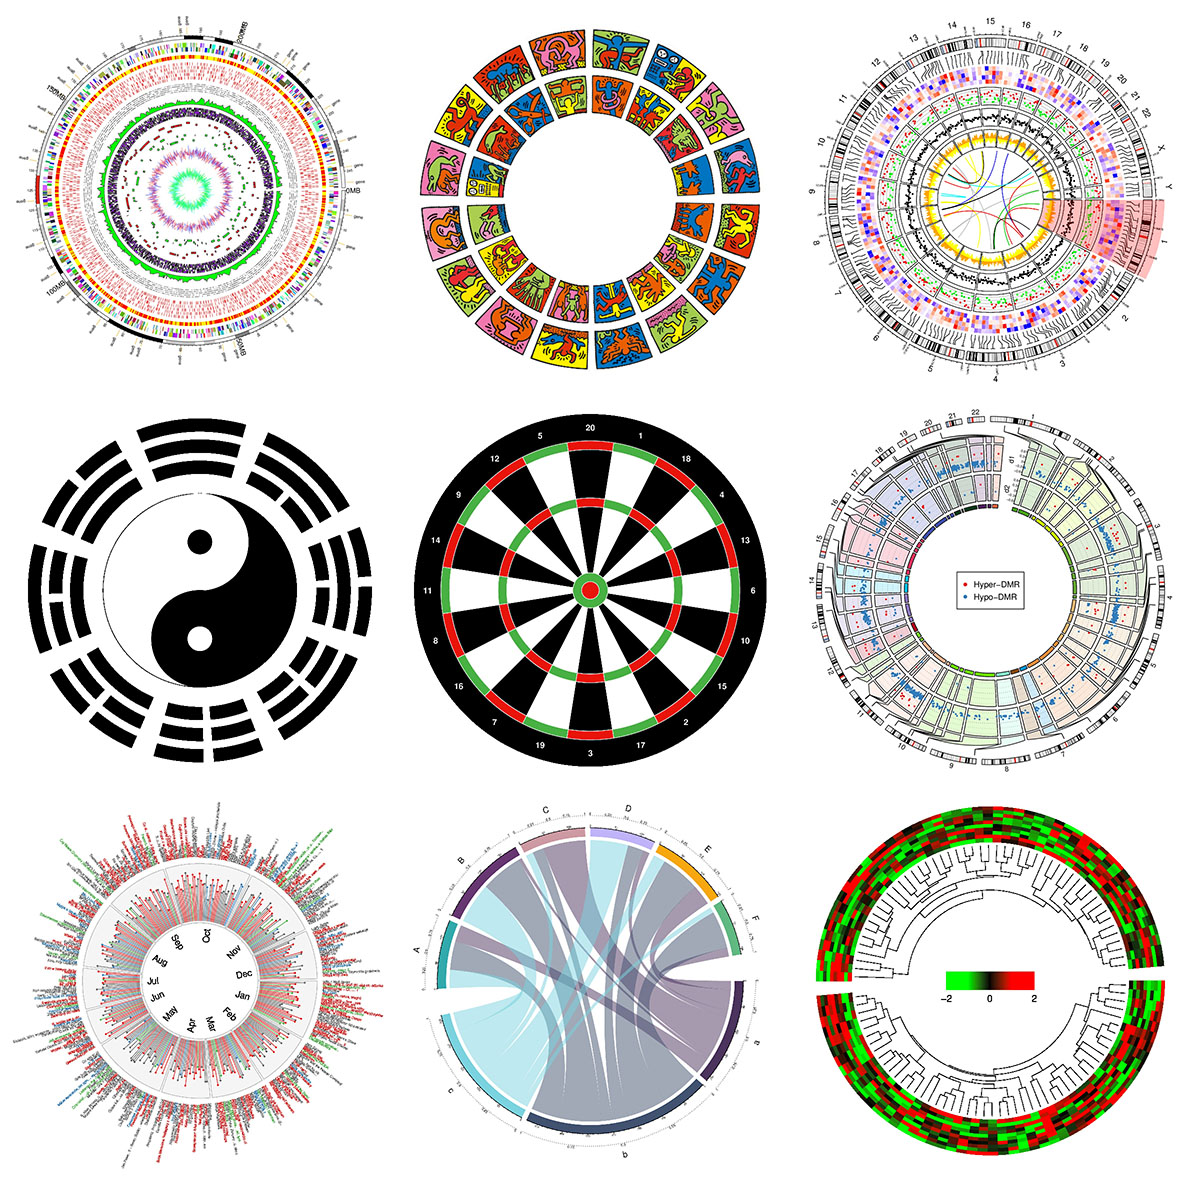
\includegraphics[width=1\linewidth]{images/ciclize_examples} 

}

\caption{Examples by circlize}\label{fig:circlize-example}
\end{figure}

\section{A quick glance}\label{a-qiuck-glance}

Before we go too deep into the details, I first demonstrate a simple
example with using basic functionalities in \textbf{circlize} package to
help you to get a basic idea of how the package works.

First let's generate some random data. There needs a character vector to
represent categories, a numeric vector of x values and a vectoe of y
values.

\begin{Shaded}
\begin{Highlighting}[]
\KeywordTok{set.seed}\NormalTok{(}\DecValTok{999}\NormalTok{)}
\NormalTok{n =}\StringTok{ }\DecValTok{1000}
\NormalTok{df =}\StringTok{ }\KeywordTok{data.frame}\NormalTok{(}\DataTypeTok{factors =} \KeywordTok{sample}\NormalTok{(letters[}\DecValTok{1}\OperatorTok{:}\DecValTok{8}\NormalTok{], n, }\DataTypeTok{replace =} \OtherTok{TRUE}\NormalTok{),}
    \DataTypeTok{x =} \KeywordTok{rnorm}\NormalTok{(n), }\DataTypeTok{y =} \KeywordTok{runif}\NormalTok{(n))}
\end{Highlighting}
\end{Shaded}

First we initialize the circular layout. The circle is split into
sectors based on the data range on x-axes in each category. In following
code, \texttt{df\$x} is split by \texttt{df\$factors} and the width of
sectors are automatically calculated based on data ranges in each
category. Be default, sectors are positioned started from \(\theta = 0\)
(in the polar coordinate system) and go along the circle clock-wisely.
You may not see anything after running following code because no track
has been added yet.

\begin{Shaded}
\begin{Highlighting}[]
\KeywordTok{library}\NormalTok{(circlize)}
\KeywordTok{circos.par}\NormalTok{(}\StringTok{"track.height"}\NormalTok{ =}\StringTok{ }\FloatTok{0.1}\NormalTok{)}
\KeywordTok{circos.initialize}\NormalTok{(}\DataTypeTok{factors =}\NormalTok{ df}\OperatorTok{$}\NormalTok{factors, }\DataTypeTok{x =}\NormalTok{ df}\OperatorTok{$}\NormalTok{x)}
\end{Highlighting}
\end{Shaded}

We set a global parameter \texttt{track.height} to 0.1 by the option
function \texttt{circis.par()} so that all tracks which will be added
have a default height of 0.1. The circle used by \textbf{circlize}
always has a radius of 1, so a height of 0.1 means 10\% of the circle
radius.

Note that the allocation of sectors only needs values on x direction (or
on the circular direction), the values on y direction (radical
direction) will be used in the step of creating tracks.

After the circular layout is initialized, graphics can be added to the
plot in a track-by-track manner. Before drawing anything, we need to
know that all tracks should be first created by
\texttt{circos.trackPlotRegion()} or, for short,
\texttt{circos.track()}, then the low-level functions can be added
afterwards. Just think in the base R graphic engine, you need first call
\texttt{plot()} then you can use functions such as \texttt{points()} and
\texttt{lines()} to add graphics. Since x ranges for cells in the track
have already been defined in the initialization step, here we only need
to specify the y ranges for each cell. The y ranges can be specified by
\texttt{y} argument as a numeric vector (so that y ranges will be
automatically extracted and calculated in each cell) or \texttt{ylim}
argument as a vector of length two. In principle, y ranges should be
same for all cells in a same track. (See Figure
\ref{fig:circlize-glance-track-1})

\begin{Shaded}
\begin{Highlighting}[]
\KeywordTok{circos.track}\NormalTok{(}\DataTypeTok{factors =}\NormalTok{ df}\OperatorTok{$}\NormalTok{factors, }\DataTypeTok{y =}\NormalTok{ df}\OperatorTok{$}\NormalTok{y,}
    \DataTypeTok{panel.fun =} \ControlFlowTok{function}\NormalTok{(x, y) \{}
        \KeywordTok{circos.text}\NormalTok{(CELL_META}\OperatorTok{$}\NormalTok{xcenter, CELL_META}\OperatorTok{$}\NormalTok{cell.ylim[}\DecValTok{2}\NormalTok{] }\OperatorTok{+}\StringTok{ }\KeywordTok{uy}\NormalTok{(}\DecValTok{5}\NormalTok{, }\StringTok{"mm"}\NormalTok{), }
\NormalTok{            CELL_META}\OperatorTok{$}\NormalTok{sector.index)}
        \KeywordTok{circos.axis}\NormalTok{(}\DataTypeTok{labels.cex =} \FloatTok{0.6}\NormalTok{)}
\NormalTok{\})}
\NormalTok{col =}\StringTok{ }\KeywordTok{rep}\NormalTok{(}\KeywordTok{c}\NormalTok{(}\StringTok{"#FF0000"}\NormalTok{, }\StringTok{"#00FF00"}\NormalTok{), }\DecValTok{4}\NormalTok{)}
\KeywordTok{circos.trackPoints}\NormalTok{(df}\OperatorTok{$}\NormalTok{factors, df}\OperatorTok{$}\NormalTok{x, df}\OperatorTok{$}\NormalTok{y, }\DataTypeTok{col =}\NormalTok{ col, }\DataTypeTok{pch =} \DecValTok{16}\NormalTok{, }\DataTypeTok{cex =} \FloatTok{0.5}\NormalTok{)}
\KeywordTok{circos.text}\NormalTok{(}\OperatorTok{-}\DecValTok{1}\NormalTok{, }\FloatTok{0.5}\NormalTok{, }\StringTok{"text"}\NormalTok{, }\DataTypeTok{sector.index =} \StringTok{"a"}\NormalTok{, }\DataTypeTok{track.index =} \DecValTok{1}\NormalTok{)}
\end{Highlighting}
\end{Shaded}

\begin{figure}

{\centering 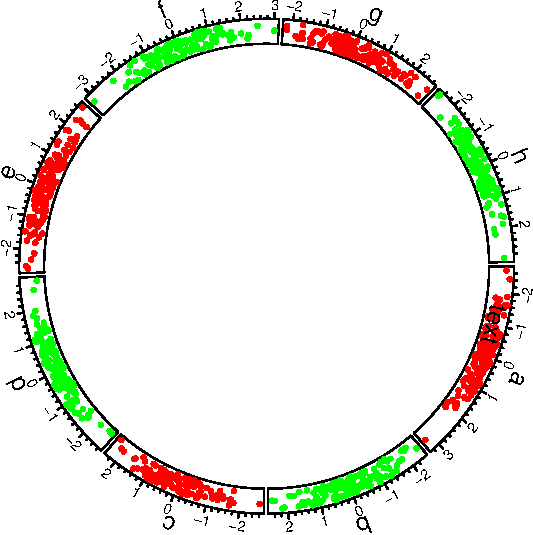
\includegraphics{01-introduction_files/figure-latex/circlize-glance-track-1-1} 

}

\caption{First example of circlize, add the first track.}\label{fig:circlize-glance-track-1}
\end{figure}

Axes for the circular plot are normally drawn on the most outside of the
circle. Here we add axes in the first track by putting
\texttt{circos.axis()} inside the self-defined function
\texttt{panel.fun} (see the code above). \texttt{circos.track()} creates
plotting region in a cell-by-cell manner and the \texttt{panel.fun} is
actually executed immediately after the plotting region for a certain
cell is created. Thus, \texttt{panel.fun} actually means adding graphics
in the ``current cell'' (Usage of \texttt{panel.fun} is further
discussed in Section \ref{panel-fun}). Without specifying any arguments,
\texttt{circos.axis()} draws x-axes on the top of each cell (or the
outside of each cell).

Also, we add sector name outside the first track by using
\texttt{circos.text()}. \texttt{CELL\_META} provides ``meta
information'' for the current cell. There are several parameters which
can be retrieved by \texttt{CELL\_META}. All its usage is explained in
Section \ref{panel-fun}. In above code, the sector names are drawn
outside the cells and you may see warning messages saying data points
exceeding the plotting regions. That is total fine and no worry about
it. You can also add sector names by creating an empty track without
borders as the first track and add sector names in it (like what
\texttt{circos.initializeWithIdeogram()} and \texttt{chordDiagram()} do,
after you go through following chapters).

When specifying the position of text on the y direction, an offset of
\texttt{uy(5,\ "mm")} is added to the y position of the text. In
\texttt{circos.text()}, x and y values are measured in the data
coordinate (the coordinate in cell), and \texttt{uy()} function (or
\texttt{ux()} which is measured on x direction) converts absolute units
to corresponding values in data coordinate. Section
\ref{convert-functions} provides more information of converting units in
different coordinates.

After the track is created, points are added to the first track by
\texttt{circos.trackPoints()}. \texttt{circos.trackPoints()} simply adds
points in all cells simultaneously. As further explained in Section
\ref{points}, it can be replaced by putting \texttt{circos.text()} in
\texttt{panel.fun}, however, \texttt{circos.trackPoints()} would be more
convenient if only the points are needed to put in the cells. It is
quite straightforward to understand that this function needs a
categorical variable (\texttt{df\$factors}), values on x direction and y
direction (\texttt{df\$x} and \texttt{df\$y}).

Low-level functions such as \texttt{circos.text()} can also be used
outside \texttt{panel.fun} as shown in above code. If so,
\texttt{sector.index} and \texttt{track.index} need to be specified
explicitly because the ``current'' sector and ``current'' track may not
be what you want. If the graphics are directly added to the track which
are most recently created, \texttt{track.index} can be ommitted because
this track is just marked as the ``current'' track.

OK, now we add histograms to the second track. Here
\texttt{circos.trackHist()} is a high- level function which means it
creates a new track (as you can imagin \texttt{hist()} is also a
high-level function). \texttt{bin.size} is explicitly set so that the
bin size for histograms in all cells are the same and can be compared to
each other. (See Figure \ref{fig:circlize-glance-track-2})

\begin{Shaded}
\begin{Highlighting}[]
\NormalTok{bgcol =}\StringTok{ }\KeywordTok{rep}\NormalTok{(}\KeywordTok{c}\NormalTok{(}\StringTok{"#EFEFEF"}\NormalTok{, }\StringTok{"#CCCCCC"}\NormalTok{), }\DecValTok{4}\NormalTok{)}
\KeywordTok{circos.trackHist}\NormalTok{(df}\OperatorTok{$}\NormalTok{factors, df}\OperatorTok{$}\NormalTok{x, }\DataTypeTok{bin.size =} \FloatTok{0.2}\NormalTok{, }\DataTypeTok{bg.col =}\NormalTok{ bgcol, }\DataTypeTok{col =} \OtherTok{NA}\NormalTok{)}
\end{Highlighting}
\end{Shaded}

\begin{figure}

{\centering 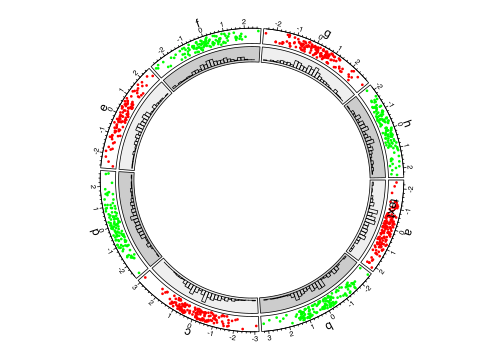
\includegraphics{01-introduction_files/figure-latex/circlize-glance-track-2-1} 

}

\caption{First example of circlize, add the second track.}\label{fig:circlize-glance-track-2}
\end{figure}

In the third track and in \texttt{panel.fun}, we randomly picked 10 data
points in each cell, sort them and connect them with lines. In following
code, when \texttt{factors}, \texttt{x} and \texttt{y} arguments are set
in \texttt{circos.track()}, x values and y values are split by
\texttt{df\$factors} and corresponding subset of x and y values are sent
to \texttt{panel.fun} through \texttt{panel.fun}'s \texttt{x} and
\texttt{y} arguments. Thus, \texttt{x} an \texttt{y} in
\texttt{panel.fun} are exactly the values in the ``current'' cell. (See
Figure \ref{fig:circlize-glance-track-3})

\begin{Shaded}
\begin{Highlighting}[]
\KeywordTok{circos.track}\NormalTok{(}\DataTypeTok{factors =}\NormalTok{ df}\OperatorTok{$}\NormalTok{factors, }\DataTypeTok{x =}\NormalTok{ df}\OperatorTok{$}\NormalTok{x, }\DataTypeTok{y =}\NormalTok{ df}\OperatorTok{$}\NormalTok{y,}
    \DataTypeTok{panel.fun =} \ControlFlowTok{function}\NormalTok{(x, y) \{}
\NormalTok{        ind =}\StringTok{ }\KeywordTok{sample}\NormalTok{(}\KeywordTok{length}\NormalTok{(x), }\DecValTok{10}\NormalTok{)}
\NormalTok{        x2 =}\StringTok{ }\NormalTok{x[ind]}
\NormalTok{        y2 =}\StringTok{ }\NormalTok{y[ind]}
\NormalTok{        od =}\StringTok{ }\KeywordTok{order}\NormalTok{(x2)}
        \KeywordTok{circos.lines}\NormalTok{(x2[od], y2[od])}
\NormalTok{\})}
\end{Highlighting}
\end{Shaded}

\begin{figure}

{\centering 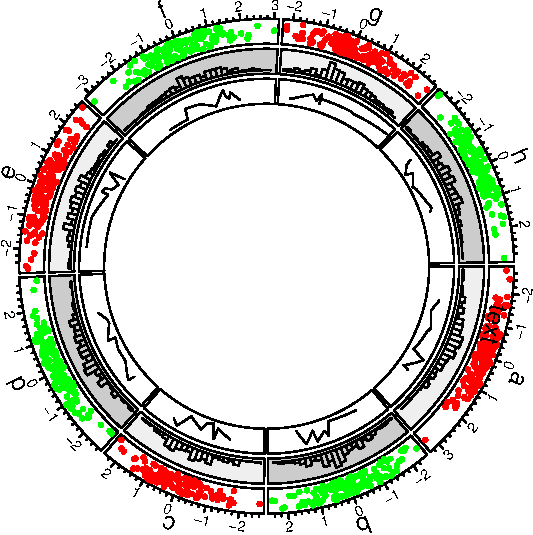
\includegraphics{01-introduction_files/figure-latex/circlize-glance-track-3-1} 

}

\caption{First example of circlize, add the third track.}\label{fig:circlize-glance-track-3}
\end{figure}

Now we go back to the second track and update the cell in sector ``d''.
This is done by \texttt{circos.updatePlotRegion()} or the short version
\texttt{circos.update()}. The function erases graphics which have been
added. \texttt{circos.update()} can not modify the \texttt{xlim} and
\texttt{ylim} of the cell as well as other settings related to the
position of the cell. \texttt{circos.update()} needs to explicitly
specify the sector index and track index unless the ``current'' cell is
what you want to update. After the calling of \texttt{circos.update()},
the ``current'' cell is redirected to the cell you just specified and
you can use low-level graphic functions to add graphics directly into
it. (See Figure \ref{fig:circlize-glance-track-update})

\begin{Shaded}
\begin{Highlighting}[]
\KeywordTok{circos.update}\NormalTok{(}\DataTypeTok{sector.index =} \StringTok{"d"}\NormalTok{, }\DataTypeTok{track.index =} \DecValTok{2}\NormalTok{, }
    \DataTypeTok{bg.col =} \StringTok{"#FF8080"}\NormalTok{, }\DataTypeTok{bg.border =} \StringTok{"black"}\NormalTok{)}
\KeywordTok{circos.points}\NormalTok{(}\DataTypeTok{x =} \OperatorTok{-}\DecValTok{2}\OperatorTok{:}\DecValTok{2}\NormalTok{, }\DataTypeTok{y =} \KeywordTok{rep}\NormalTok{(}\FloatTok{0.5}\NormalTok{, }\DecValTok{5}\NormalTok{), }\DataTypeTok{col =} \StringTok{"white"}\NormalTok{)}
\KeywordTok{circos.text}\NormalTok{(CELL_META}\OperatorTok{$}\NormalTok{xcenter, CELL_META}\OperatorTok{$}\NormalTok{ycenter, }\StringTok{"updated"}\NormalTok{, }\DataTypeTok{col =} \StringTok{"white"}\NormalTok{)}
\end{Highlighting}
\end{Shaded}

\begin{figure}

{\centering 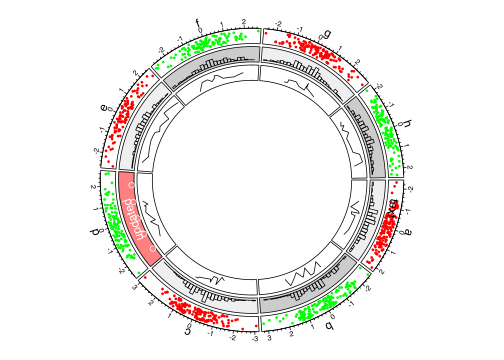
\includegraphics{01-introduction_files/figure-latex/circlize-glance-track-update-1} 

}

\caption{First example of circlize, update the second track.}\label{fig:circlize-glance-track-update}
\end{figure}

Next we continue to create new tracks. Although we have gone back to the
second track, when creating a new track, the new track is still created
after the track which is most inside. In this new track, we add heatmaps
by \texttt{circos.rect()}. Note here we haven't set the input data,
while simply set \texttt{ylim} argument because heatmaps just fill the
whole cell from the most left to right and from bottom to top. Also the
exact value of \texttt{ylim} is not important and \texttt{x}, \texttt{y}
in \texttt{panel.fun()} are not used (actually they are both
\texttt{NULL}). (See Figure \ref{fig:circlize-glance-track-4})

\begin{Shaded}
\begin{Highlighting}[]
\KeywordTok{circos.track}\NormalTok{(}\DataTypeTok{ylim =} \KeywordTok{c}\NormalTok{(}\DecValTok{0}\NormalTok{, }\DecValTok{1}\NormalTok{), }\DataTypeTok{panel.fun =} \ControlFlowTok{function}\NormalTok{(x, y) \{}
\NormalTok{    xlim =}\StringTok{ }\NormalTok{CELL_META}\OperatorTok{$}\NormalTok{xlim}
\NormalTok{    ylim =}\StringTok{ }\NormalTok{CELL_META}\OperatorTok{$}\NormalTok{ylim}
\NormalTok{    breaks =}\StringTok{ }\KeywordTok{seq}\NormalTok{(xlim[}\DecValTok{1}\NormalTok{], xlim[}\DecValTok{2}\NormalTok{], }\DataTypeTok{by =} \FloatTok{0.1}\NormalTok{)}
\NormalTok{    n_breaks =}\StringTok{ }\KeywordTok{length}\NormalTok{(breaks)}
    \KeywordTok{circos.rect}\NormalTok{(breaks[}\OperatorTok{-}\NormalTok{n_breaks], }\KeywordTok{rep}\NormalTok{(ylim[}\DecValTok{1}\NormalTok{], n_breaks }\OperatorTok{-}\StringTok{ }\DecValTok{1}\NormalTok{),}
\NormalTok{                breaks[}\OperatorTok{-}\DecValTok{1}\NormalTok{], }\KeywordTok{rep}\NormalTok{(ylim[}\DecValTok{2}\NormalTok{], n_breaks }\OperatorTok{-}\StringTok{ }\DecValTok{1}\NormalTok{),}
                \DataTypeTok{col =} \KeywordTok{rand_color}\NormalTok{(n_breaks), }\DataTypeTok{border =} \OtherTok{NA}\NormalTok{)}
\NormalTok{\})}
\end{Highlighting}
\end{Shaded}

\begin{figure}

{\centering 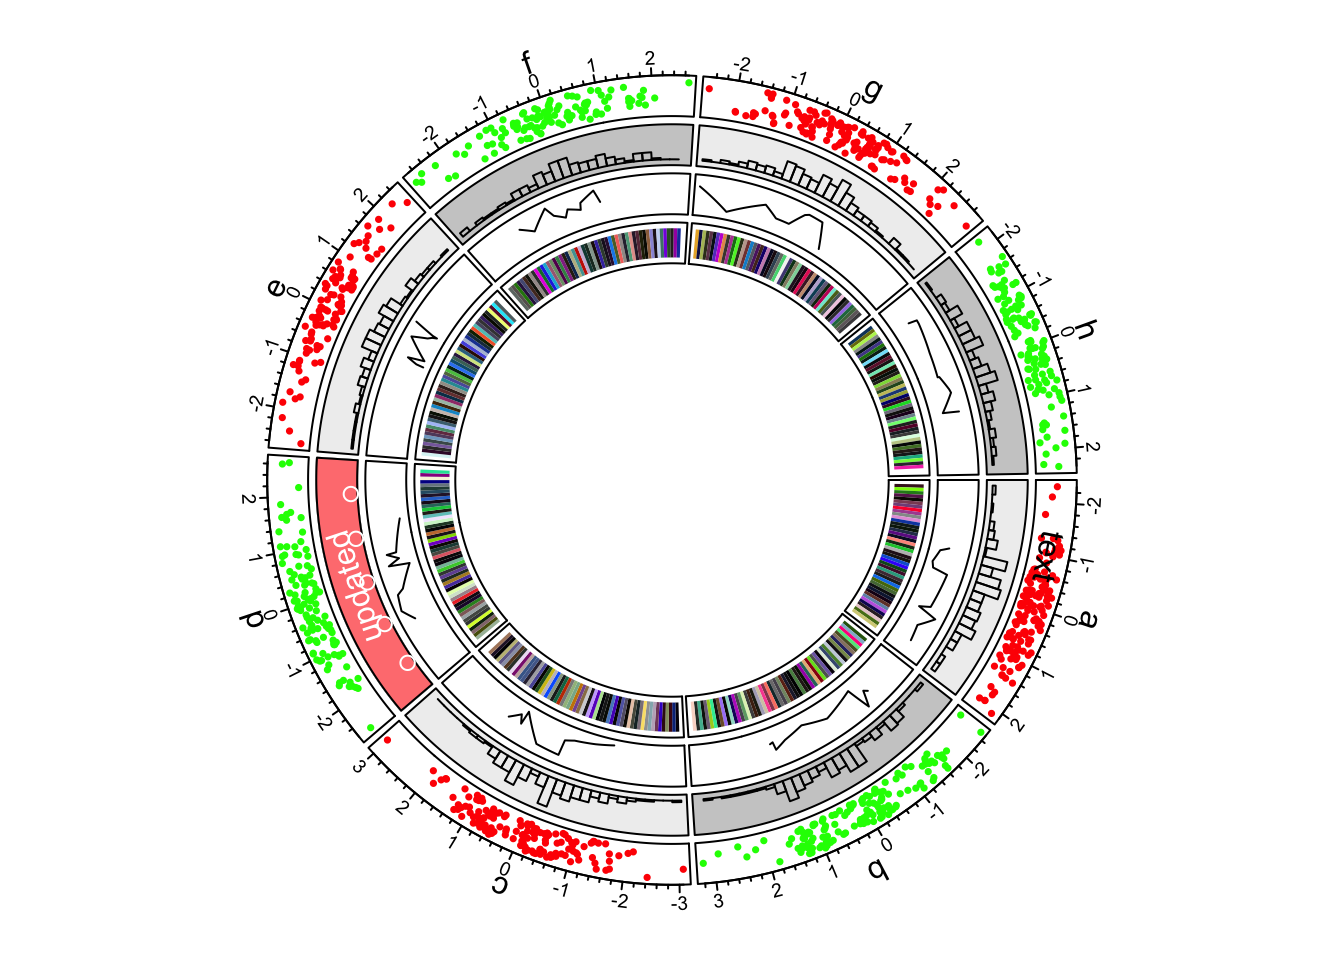
\includegraphics{01-introduction_files/figure-latex/circlize-glance-track-4-1} 

}

\caption{First example of circlize, add the fourth track.}\label{fig:circlize-glance-track-4}
\end{figure}

In the most inside of the circle, links or ribbons are added. There can
be links from single point to point, point to interval or interval to
interval. Section \ref{links} gives detailed usage of links. (See Figure
\ref{fig:circlize-glance-track-links})

\begin{Shaded}
\begin{Highlighting}[]
\KeywordTok{circos.link}\NormalTok{(}\StringTok{"a"}\NormalTok{, }\DecValTok{0}\NormalTok{, }\StringTok{"b"}\NormalTok{, }\DecValTok{0}\NormalTok{, }\DataTypeTok{h =} \FloatTok{0.4}\NormalTok{)}
\KeywordTok{circos.link}\NormalTok{(}\StringTok{"c"}\NormalTok{, }\KeywordTok{c}\NormalTok{(}\OperatorTok{-}\FloatTok{0.5}\NormalTok{, }\FloatTok{0.5}\NormalTok{), }\StringTok{"d"}\NormalTok{, }\KeywordTok{c}\NormalTok{(}\OperatorTok{-}\FloatTok{0.5}\NormalTok{,}\FloatTok{0.5}\NormalTok{), }\DataTypeTok{col =} \StringTok{"red"}\NormalTok{,}
    \DataTypeTok{border =} \StringTok{"blue"}\NormalTok{, }\DataTypeTok{h =} \FloatTok{0.2}\NormalTok{)}
\KeywordTok{circos.link}\NormalTok{(}\StringTok{"e"}\NormalTok{, }\DecValTok{0}\NormalTok{, }\StringTok{"g"}\NormalTok{, }\KeywordTok{c}\NormalTok{(}\OperatorTok{-}\DecValTok{1}\NormalTok{,}\DecValTok{1}\NormalTok{), }\DataTypeTok{col =} \StringTok{"green"}\NormalTok{, }\DataTypeTok{border =} \StringTok{"black"}\NormalTok{, }\DataTypeTok{lwd =} \DecValTok{2}\NormalTok{, }\DataTypeTok{lty =} \DecValTok{2}\NormalTok{)}
\end{Highlighting}
\end{Shaded}

\begin{figure}

{\centering 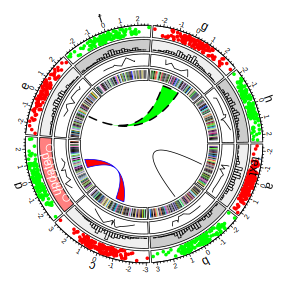
\includegraphics{01-introduction_files/figure-latex/circlize-glance-track-links-1} 

}

\caption{First example of circlize, add links.}\label{fig:circlize-glance-track-links}
\end{figure}

Finally we need to reset the graphic parameters and internal variables,
so that it will not mess up your next plot.

\begin{Shaded}
\begin{Highlighting}[]
\KeywordTok{circos.clear}\NormalTok{()}
\end{Highlighting}
\end{Shaded}

\chapter{Circular layout}\label{circular-layout}

\section{Coordinate transformation}\label{coordinate-transformation}

To map graphics onto the circle, there exist transformations from
several coordinate systems. First, there are \textbf{data coordinate
systems} in which ranges for x-axes and y-axes are the ranges of
original data. Second, there is a \textbf{polar coordinate system} in
which these coordinates are mapped onto a circle. Finally, there is a
\textbf{canvas coordinate system} in which graphics are really drawn on
the graphical device (figure \ref{fig:coordinate-transformation}). Each
cell has its own data coordinate and they are independent.
\textbf{circlize} first transforms coordinates from data coordinate
system to polar coordinate system and finally transforms into canvas
coordinate system. For users, they only need to imagine that each cell
is a normal rectangular plotting region (data coordinate) in which x-lim
and y-lim are ranges of data in that cell. \textbf{circlize} knows which
cell you are in and does all the transformations automatically.

\begin{figure}

{\centering 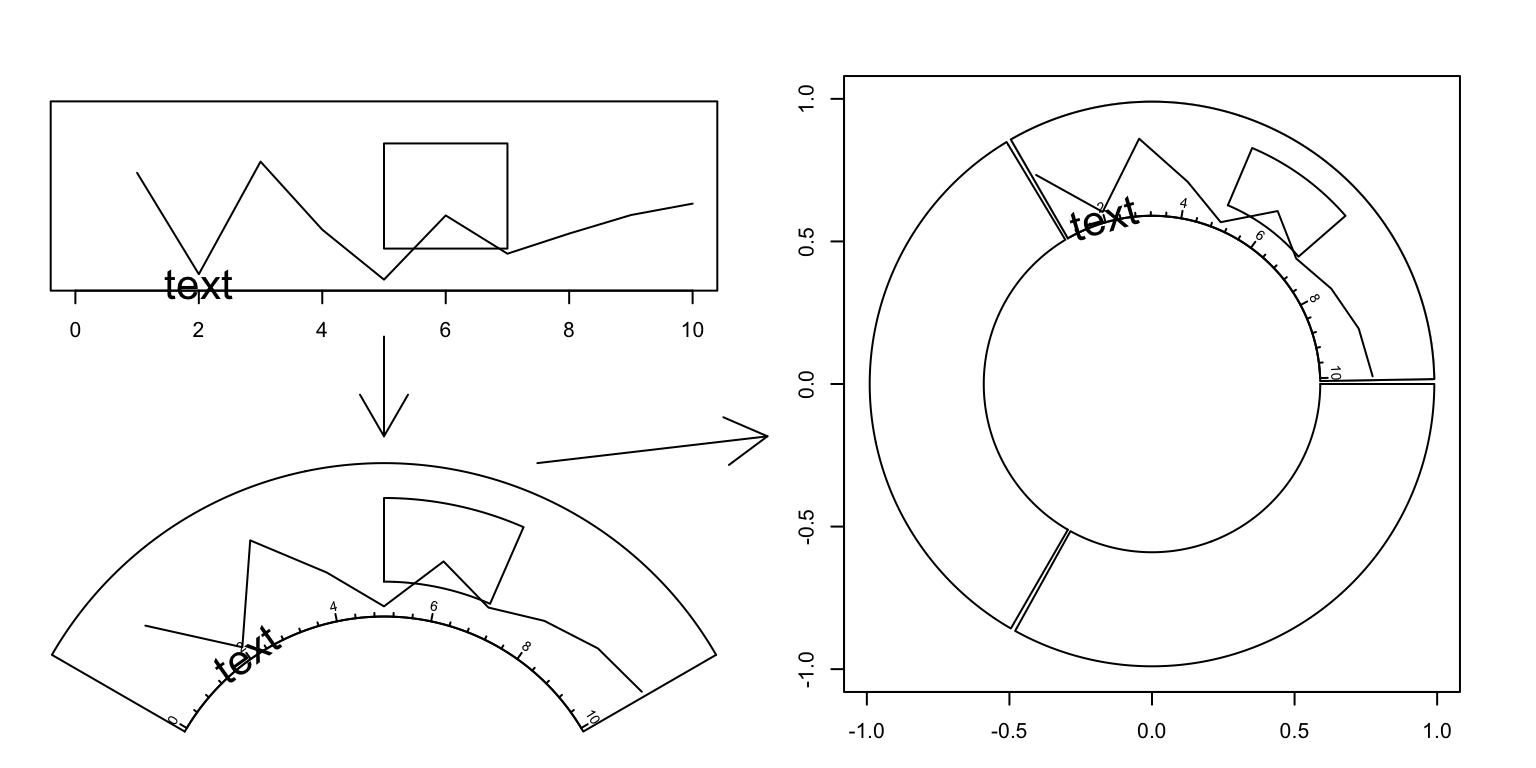
\includegraphics{02-circlize-layout_files/figure-latex/coordinate-transformation-1} 

}

\caption{Transformation between different coordinates}\label{fig:coordinate-transformation}
\end{figure}

The final canvas coordinate is in fact an ordinary coordinate in the
base R graphic system with x range in \texttt{(-1,\ 1)} and y range in
\texttt{(-1,\ 1)} by default. It should be noted that \textbf{the
circular plot is always drawn inside the circle which has radius of 1
(which means it is always a unit circle), and from outside to inside}.

\section{Rules for making the circular
plot}\label{rules-for-making-the-circular-plot}

The rule for making the circular plot is rather simple. It follows the
sequence of
\texttt{initialize\ layout\ -\textgreater{}\ create\ track\ -\textgreater{}\ add\ graphics\ -\textgreater{}\ create\ track\ -\textgreater{}\ add\ graphics\ -\ ...\ -\textgreater{}\ clear}.
Graphics can be added at any time as long as the tracks are created.
Details are shown in Figure \ref{fig:circlize-order} and as follows:

\begin{figure}

{\centering 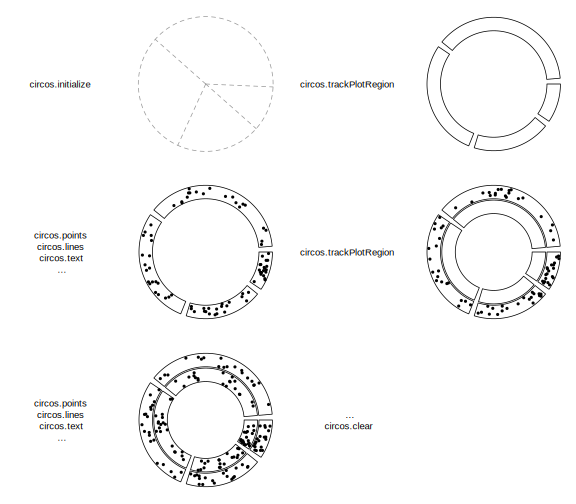
\includegraphics{02-circlize-layout_files/figure-latex/circlize-order-1} 

}

\caption{Order of drawing circular layout.}\label{fig:circlize-order}
\end{figure}

\begin{enumerate}
\def\labelenumi{\arabic{enumi}.}
\item
  Initialize the layout using \texttt{circos.initialize()}. Since
  circular layout in fact visualizes data which is in categories, there
  must be at least a categorical variable. Ranges of x values on each
  category can be specified as a vector or the range itself. See Section
  \ref{sectors-and-tracks}.
\item
  Create plotting regions for the new track and add graphics. The new
  track is created just inside the previously created one. Only after
  the creation of the track can you add other graphics on it. There are
  three ways to add graphics in cells.

  \begin{itemize}
  \tightlist
  \item
    After the creation of the track, use low-level graphic function like
    \texttt{circos.points()}, \texttt{circos.lines()}, \ldots{} to add
    graphics cell by cell. It always involves a \texttt{for} loop and
    you need to subset the data by the categorical variable manually.
  \item
    Use \texttt{circos.trackPoints()}, \texttt{circos.trackLines()},
    \ldots{} to add simple graphics through all cells simultaneously.
  \item
    Use \texttt{panel.fun} argument in \texttt{circos.track()} to add
    graphics immediately after the creation of a certain cell.
    \texttt{panel.fun} needs two arguments \texttt{x} and \texttt{y}
    which are x values and y values that are in the current cell. This
    subset operation is applied automatically. This is the most
    recommended way. Section \ref{panel-fun} gives detailed explanation
    of using \texttt{panel.fun} argument.
  \end{itemize}
\item
  Repeat step 2 to add more tracks on the circle unless it reaches the
  center of the circle.
\item
  Call \texttt{circos.clear()} to clean up.
\end{enumerate}

As mentioned above, there are three ways to add graphics on a track.

\begin{enumerate}
\def\labelenumi{\arabic{enumi}.}
\item
  Create plotting regions for the whole track first and then add
  graphics by specifying \texttt{sector.index}. In the following pseudo
  code, \texttt{x1}, \texttt{y1} are data points in a given cell, which
  means you need to do data subsetting manually.

  In following code, \texttt{circos.points()} and
  \texttt{circos.lines()} are used separatedly from
  \texttt{circos.track()}, thus, the index for the sector needs to be
  explicitly specified by \texttt{sector.index} argument. There is also
  a \texttt{track.index} argument for both functions, however, the
  default value is the ``current'' track index and as the two functions
  are used just after \texttt{circos.track()}, the ``current'' track
  index is what the two functions expect and it can be ommited when
  calling the two functions.
\end{enumerate}

\begin{Shaded}
\begin{Highlighting}[]
\KeywordTok{circos.initialize}\NormalTok{(factors, xlim)}
\KeywordTok{circos.track}\NormalTok{(factors, ylim)}
\ControlFlowTok{for}\NormalTok{(sector.index }\ControlFlowTok{in}\NormalTok{ all.sector.index) \{}
    \KeywordTok{circos.points}\NormalTok{(x1, y1, sector.index)}
    \KeywordTok{circos.lines}\NormalTok{(x2, y2, sector.index)}
\NormalTok{\}}
\end{Highlighting}
\end{Shaded}

\begin{enumerate}
\def\labelenumi{\arabic{enumi}.}
\setcounter{enumi}{1}
\item
  Add graphics in a batch mode. In following code,
  \texttt{circos.trackPoints()} and \texttt{circos.trackLines()} need a
  categorical variable, a vector of x values and a vector of y values. X
  and y values will be split by the categorical variable and sent to
  corresponding cell to add the graphics. Internally, this is done by
  using \texttt{circos.points()} or \texttt{circos.lines()} in a
  \texttt{for} loop. This way to add graphics would be convenient if
  users only want to add a specific type of simple graphics (e.g.~only
  points) to the track, but it is not recommended for making complex
  graphics.

  \texttt{circos.trackPoints()} and \texttt{circos.trackLines()} need a
  \texttt{track.index} to specify which track to add the graphics.
  Similarly, since these two are called just after
  \texttt{circos.track()}, the graphics are added in the newly created
  track right away.
\end{enumerate}

\begin{Shaded}
\begin{Highlighting}[]
\KeywordTok{circos.initialize}\NormalTok{(factors, xlim)}
\KeywordTok{circos.track}\NormalTok{(factors, ylim)}
\KeywordTok{circos.trackPoints}\NormalTok{(factors, x, y)}
\KeywordTok{circos.trackLines}\NormalTok{(factors, x, y)}
\end{Highlighting}
\end{Shaded}

\begin{enumerate}
\def\labelenumi{\arabic{enumi}.}
\setcounter{enumi}{2}
\item
  Use a panel function to add self-defined graphics as soon as the cell
  has been created. This is the way recommended and you can find most of
  the code in this book uses \texttt{panel.fun}. \texttt{circos.track()}
  creates cells one by one and after the creation of a cell, and
  \texttt{panel.fun} is executed on this cell immediately. In this case,
  the ``current'' sector and ``current'' track are marked to this cell
  that you can directly use low-level functions without specifying
  sector index and track index.

  If you look at following code, you will find the code inside
  \texttt{panel.fun} is as natural as using \texttt{points()} or
  \texttt{lines()} in the normal R graphic system. This is a way to help
  you think a cell is an ``imaginary rectangular plotting region''.
\end{enumerate}

\begin{Shaded}
\begin{Highlighting}[]
\KeywordTok{circos.initialize}\NormalTok{(factors, xlim)}
\KeywordTok{circos.track}\NormalTok{(factors, all_x, all_y, ylim,}
    \DataTypeTok{panel.fun =} \ControlFlowTok{function}\NormalTok{(x, y) \{}
        \KeywordTok{circos.points}\NormalTok{(x, y)}
        \KeywordTok{circos.lines}\NormalTok{(x, y)}
\NormalTok{\})}
\end{Highlighting}
\end{Shaded}

There are several internal variables keeping tracing of the current
sector and track when applying \texttt{circos.track()} and
\texttt{circos.update()}. Thus, although functions like
\texttt{circos.points()}, \texttt{circos.lines()} need to specify the
index of sector and track, they will take the current one by default. As
a result, if you draw points, lines, text \emph{et al} just after the
creation of the track or cell, you do not need to set the sector index
and the track index explicitly and it will be added in the most recently
created or updated cell.

\section{Sectors and tracks}\label{sectors-and-tracks}

A circular layout is composed of sectors and tracks. As illustrated in
Figure \ref{fig:circlize-coordinate}, the red circle is one track and
the blue represents one sector. The intersection of a sector and a track
is called a cell which can be thought as an imaginary plotting region
for data points. In this section, we introduce how to set data ranges on
x and y directions in cells.

\begin{figure}

{\centering 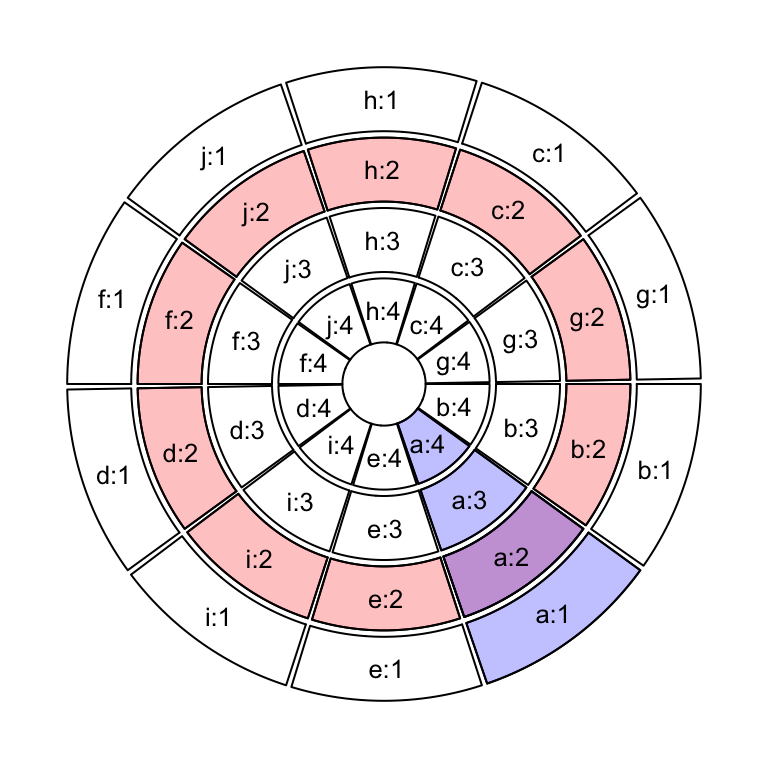
\includegraphics{02-circlize-layout_files/figure-latex/circlize-coordinate-1} 

}

\caption{Sectors and tracks in circular layout.}\label{fig:circlize-coordinate}
\end{figure}

Sectors are first allocated on the circle by
\texttt{circos.initialize()}. There must be a categorical variable (say
\texttt{factors}) that on the circle, each sector corresponds to one
category. The width of sectors (measured by degree) are proportional to
the data range in sectors on x direction (or the circular direction).
The data range can be specified as a numeric vector \texttt{x} which has
same length as \texttt{factors}, then \texttt{x} is split by
\texttt{factors} and data ranges are calculated for each sector
internally.

Data ranges can also be specified directly by \texttt{xlim} argument.
The valid value for \texttt{xilm} is a two-column matrix with same
number of rows as number of sectors that each row in \texttt{xlim}
corresponds to one sector. If \texttt{xlim} has row names which already
cover sector names, row order of \texttt{xlim} is automatically
adjusted. If \texttt{xlim} is a vector of length two, all sectors have
the same x range.

\begin{Shaded}
\begin{Highlighting}[]
\KeywordTok{circos.initialize}\NormalTok{(factors, }\DataTypeTok{x =}\NormalTok{ x)}
\KeywordTok{circos.initialize}\NormalTok{(factors, }\DataTypeTok{xlim =}\NormalTok{ xlim)}
\end{Highlighting}
\end{Shaded}

After the initialization of the layout, you may not see anything drawn
or only an empty graphical device is opened. That is because no track
has been created yet, however, the layout has already been recorded
internally.

In the initialization step, not only the width of each sector is
assigned, but also the order of sectors on the circle is determined.
\textbf{Order of the sectors are determined by the order of levels of
the input factor}. If the value for \texttt{factors} is not a factor,
the order of sectors is \texttt{unique(factors)}. Thus, if you want to
change the order of sectors, you can just change of the level of
\texttt{factors} variable. The following code generates plots with
different sector orders (Figure \ref{fig:circlize-factor}).

\begin{Shaded}
\begin{Highlighting}[]
\NormalTok{fa =}\StringTok{ }\KeywordTok{c}\NormalTok{(}\StringTok{"d"}\NormalTok{, }\StringTok{"f"}\NormalTok{, }\StringTok{"e"}\NormalTok{, }\StringTok{"c"}\NormalTok{, }\StringTok{"g"}\NormalTok{, }\StringTok{"b"}\NormalTok{, }\StringTok{"a"}\NormalTok{)}
\NormalTok{f1 =}\StringTok{ }\KeywordTok{factor}\NormalTok{(fa)}
\KeywordTok{circos.initialize}\NormalTok{(}\DataTypeTok{factors =}\NormalTok{ f1, }\DataTypeTok{xlim =} \KeywordTok{c}\NormalTok{(}\DecValTok{0}\NormalTok{, }\DecValTok{1}\NormalTok{))}
\NormalTok{f2 =}\StringTok{ }\KeywordTok{factor}\NormalTok{(fa, }\DataTypeTok{levels =}\NormalTok{ fa)}
\KeywordTok{circos.initialize}\NormalTok{(}\DataTypeTok{factors =}\NormalTok{ f2, }\DataTypeTok{xlim =} \KeywordTok{c}\NormalTok{(}\DecValTok{0}\NormalTok{, }\DecValTok{1}\NormalTok{))}
\end{Highlighting}
\end{Shaded}

\begin{figure}

{\centering 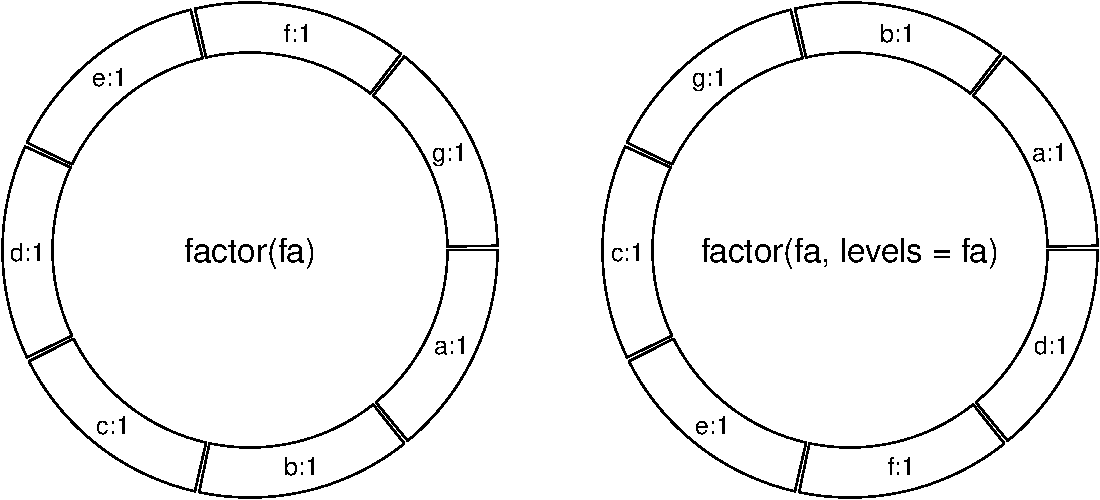
\includegraphics{02-circlize-layout_files/figure-latex/circlize-factor-1} 

}

\caption{Different sector orders.}\label{fig:circlize-factor}
\end{figure}

\textbf{In different tracks, cells in the same sector share the same
data range on x-axes.} Then, for each track, we only need to specify the
data range on y direction (or the radical direction) for cells. Similar
as \texttt{circos.initialize()}, \texttt{circos.track()} also receives
either \texttt{y} or \texttt{ylim} argument to specify the range of
y-values. Since all cells in a same track shares a same y range,
\texttt{ylim} is just a vector of length two if it is specified.

\texttt{x} can also be specified in \texttt{circos.track()}, but it is
only used to send to \texttt{panel.fun}. In Section \ref{panel-fun}, we
will introduce how \texttt{x} and \texttt{y} are sent to each cell and
how the graphics are added.

\begin{Shaded}
\begin{Highlighting}[]
\KeywordTok{circos.track}\NormalTok{(factors, }\DataTypeTok{y =}\NormalTok{ y)}
\KeywordTok{circos.track}\NormalTok{(factors, }\DataTypeTok{ylim =} \KeywordTok{c}\NormalTok{(}\DecValTok{0}\NormalTok{, }\DecValTok{1}\NormalTok{))}
\KeywordTok{circos.track}\NormalTok{(factors, }\DataTypeTok{x =}\NormalTok{ x, }\DataTypeTok{y =}\NormalTok{ y)}
\end{Highlighting}
\end{Shaded}

In the track creation step, since all sectors have already been
allocated in the circle, if \texttt{factors} argument is not set,
\texttt{circos.track()} would create plotting regions for all available
sectors. Also, levels of \texttt{factors} do not need to be specified
explicitly because the order of sectors has already be determined in the
initialization step. If users only create cells for a subset of sectors
in the track (not all sectors), in fact, cells in remaining unspecified
sectors are created as well, but with no borders (pretending they are
not created).

\begin{Shaded}
\begin{Highlighting}[]
\CommentTok{# assume `factors` only covers a subset of sectors}
\CommentTok{# You will only see cells that are covered in `factors` have borders}
\KeywordTok{circos.track}\NormalTok{(factors, }\DataTypeTok{y =}\NormalTok{ y)}
\CommentTok{# You will see all cells have borders}
\KeywordTok{circos.track}\NormalTok{(}\DataTypeTok{ylim =} \KeywordTok{ranges}\NormalTok{(y))}
\end{Highlighting}
\end{Shaded}

Cells are basic units in the circular plot and are independent from each
other. After the creation of cells, they have self-contained meta values
of x-lim and y-lim (data range measured in data coordinate). So if you
are adding graphics in one cell, you do not need to consider things
outside the cell and also you do not need to consider you are in the
circle. Just pretending it is normal rectangle region with its own
coordinate.

\begin{figure}

{\centering 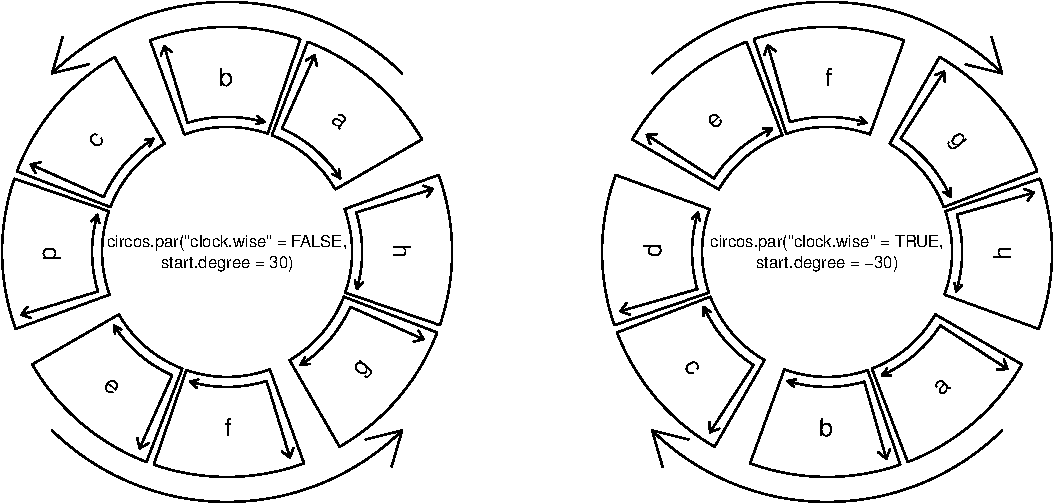
\includegraphics{02-circlize-layout_files/figure-latex/circlize-direction-1} 

}

\caption{Sector directions.}\label{fig:circlize-direction}
\end{figure}

\section{Graphic parameters}\label{graphic-parameters}

Some basic parameters for the circular layout can be set by
\texttt{circos.par()}. These parameters are listed as follows. Note some
parameters can only be modified before the initialization of the
circular layout.

\begin{itemize}
\tightlist
\item
  \texttt{start.degree}: The starting degree where the first sector is
  put. Note this degree is measured in the standard polar coordinate
  system which means it is always reverse clockwise. E.g. if it is set
  to 90, sectors start from the top center of the circle. See Figure
  \ref{fig:circlize-direction}.
\item
  \texttt{gap.degree}: Gap between two neighbour sectors. It can be a
  single value which means all gaps share same degree, or a vector which
  has same number as sectors. \textbf{Note the first gap is after the
  first sector.} See Figure \ref{fig:circlize-direction} and figure
  \ref{fig:circlize-region}.
\item
  \texttt{gap.after}: Same as \texttt{gap.degree}, but more
  understandable. Modifying values of \texttt{gap.after} will also
  modify \texttt{gap.degree} and vice versa.
\item
  \texttt{track.margin}:
  \href{https://www.w3schools.com/css/css_margin.asp}{Like
  \texttt{margin} in Cascading Style Sheets (CSS)}, it is the blank area
  out of the plotting region, also outside of the borders. Since left
  and right margin are controlled by \texttt{gap.after}, only bottom and
  top margin need to be set. The value for \texttt{track.margin} is the
  percentage to the radius of the unit circle. The value can also be set
  by \texttt{convert\_height()} or the short version \texttt{uh()}
  function with absolute units. See figure \ref{fig:circlize-region}.
\item
  \texttt{cell.padding}: Padding of the cell.
  \href{https://www.w3schools.com/css/css_padding.asp}{Like
  \texttt{padding} in Cascading Style Sheets (CSS)}, it is the blank
  area around the plotting regions, but within the borders. The
  parameter has four values, which control the bottom, left, top and
  right padding respectively. The first and the third padding values are
  the percentages to the radius of the unit circle, and the second and
  fourth values are the degrees. The first and the third value can be
  set by \texttt{uh()} with absolute units. See figure
  \ref{fig:circlize-region}.
\item
  \texttt{unit.circle.segments}: Since curves are simulated by a series
  of straight lines, this parameter controls the amount of segments to
  represent a curve. The minimal length of the line segment is the
  length of the unit circle (\(2\pi\)) divided by
  \texttt{unit.circle.segments}. More segments means better
  approximation for the curves, while generate larger file size if
  figures are in PDF format. See explanantion in Section \ref{lines}.
\item
  \texttt{track.height}: The default height of tracks. It is the
  percentage to the radius of the unit circle. The height includes the
  top and bottom cell paddings but not the margins. The value can be set
  by \texttt{uh()} with absolute units.
\item
  \texttt{points.overflow.warning}: Since each cell is in fact not a
  real plotting region but only an ordinary rectangle (or more
  precisely, a circular rectangle), it does not remove points that are
  plotted outside of the region. So if some points (or lines, text) are
  out of the plotting region, by default, the package would continue
  drawing the points but with warning messages. However, in some
  circumstances, drawing something out of the plotting region is useful,
  such as adding some text annotations (like the first track in Figure
  \ref{fig:circlize-glance-track-1}). Set this value to \texttt{FALSE}
  to turn off the warnings.
\item
  \texttt{canvas.xlim}: The ranges in the canvas coordinate in x
  direction. \textbf{circlize} is forced to put everything inside the
  unit circle, so \texttt{canvas.xlim} and \texttt{canvas.ylim} is
  \texttt{c(-1,\ 1)} by default. However, you can set it to a more broad
  interval if you want to leave more spaces out of the circle. By
  choosing proper \texttt{canvas.xlim} and \texttt{canvas.ylim},
  actually you can customize the circle. E.g. setting
  \texttt{canvas.xlim} to \texttt{c(0,\ 1)} and \texttt{canvas.ylim} to
  \texttt{c(0,\ 1)} would only draw 1/4 of the circle.
\item
  \texttt{canvas.ylim}: The ranges in the canvas coordinate in y
  direction.
\item
  \texttt{clock.wise}: The order for drawing sectors. Default is
  \texttt{TRUE} which means clockwise (figure
  \ref{fig:circlize-direction}. \textbf{Note that inside each cell, the
  direction of x-axis is always clockwise and direction of y-axis is
  always from inside to outside in the circle.}
\end{itemize}

\begin{figure}

{\centering 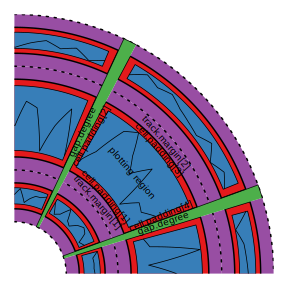
\includegraphics{02-circlize-layout_files/figure-latex/circlize-region-1} 

}

\caption{Regions in a cell.}\label{fig:circlize-region}
\end{figure}

Default values for graphic parameters are listed in following table.

\begin{longtable}[]{@{}ll@{}}
\toprule
\texttt{start.degree} & \texttt{0}\tabularnewline
\texttt{gap.degree}/\texttt{gap.after} & \texttt{1}\tabularnewline
\texttt{track.margin} & \texttt{c(0.01,\ 0.01)}\tabularnewline
\texttt{cell.padding} &
\texttt{c(0.02,\ 1.00,\ 0.02,\ 1.00)}\tabularnewline
\texttt{unit.circle.segments} & \texttt{500}\tabularnewline
\texttt{track.height} & \texttt{0.2}\tabularnewline
\texttt{points.overflow.warning} & \texttt{TRUE}\tabularnewline
\texttt{canvas.xlim} & \texttt{c(-1,\ 1)}\tabularnewline
\texttt{canvas.ylim} & \texttt{c(-1,\ 1)}\tabularnewline
\texttt{clock.wise} & \texttt{TRUE}\tabularnewline
\bottomrule
\end{longtable}

Parameters related to the allocation of sectors cannot be changed after
the initialization of the circular layout. Thus, \texttt{start.degree},
\texttt{gap.degree}/\texttt{gap.after}, \texttt{canvas.xlim},
\texttt{canvas.ylim} and \texttt{clock.wise} can only be modified before
\texttt{circos.initialize()}. The second and the fourth values of
\texttt{cell.padding} (left and right paddings) can not be modified
neither (or will be ignored).

Similar reason, since some of the parameters are defined before the
initialization of the circular layout, after making each plot, you need
to call \texttt{circos.clear()} to manually reset all the parameters.

\section{Create plotting regions}\label{create-plotting-regions}

As described above, only after creating the plotting region can you add
low- level graphics on it. The minimal set of arguments for
\texttt{circos.track()} is to set either \texttt{y} or \texttt{ylim}
which assigns range of y values for this track. \texttt{circos.track()}
creates tracks for all sectors although in some case only parts of them
are visible.

If \texttt{factors} is not specified, all cells in the track will be
created with the same settings. If \texttt{factors}, \texttt{x} and
\texttt{y} are set, they need to be vectors with the same length. Proper
values of \texttt{x} and \texttt{y} that correspond to current cell will
be passed to \texttt{panel.fun} by subsetting \texttt{factors}
internally. Section \ref{panel-fun} explains the usage of
\texttt{panel.fun}.

Graphic arguments such as \texttt{bg.border} and \texttt{bg.col} can
either be a scalar or a vector. If it is a vector, the length must be
equal to the number of sectors and the order corresponds to the order of
sectors. Thus, you can create plot regions with different styles of
borders and background colors.

If you are confused with the \texttt{factors} orders, you can also
customize the borders and background colors inside \texttt{panel.fun}.
\texttt{get.cell.meta.data("cell.xlim")} and
\texttt{get.cell.meta.data("cell.ylim")} give you dimensions of the
plotting region and you can customize plot regions directly by e.g.
\texttt{circos.rect(col\ =\ "\#FF000040",\ border\ =\ 1)}.

\texttt{circos.track()} provides \texttt{track.margin} and
\texttt{cell.padding} arguments that they only control track margins and
cell paddings for the current track. Of course the second and fourth
value in \texttt{cell.padding} are ignored.

\section{Update plotting regions}\label{update-plotting-regions}

\texttt{circos.track()} creates new tracks, however, if
\texttt{track.index} argument is set to a track which already exists,
\texttt{circos.track()} actually \textbf{re-creates} this track. In this
case, coordinates on y directions can be re-defined, but settings
related to the positions of the track such as the height of the track
can not be modified.

\begin{Shaded}
\begin{Highlighting}[]
\KeywordTok{circos.track}\NormalTok{(factors, }\DataTypeTok{ylim =} \KeywordTok{c}\NormalTok{(}\DecValTok{0}\NormalTok{, }\DecValTok{1}\NormalTok{), }\DataTypeTok{track.index =} \DecValTok{1}\NormalTok{, ...)}
\end{Highlighting}
\end{Shaded}

For a single cell, \texttt{circos.update()} can be used to erase all
graphics that have been already added in the cell. However, the data
coordinate in the cell keeps unchanged.

\begin{Shaded}
\begin{Highlighting}[]
\KeywordTok{circos.update}\NormalTok{(sector.index, track.index)}
\KeywordTok{circos.points}\NormalTok{(x, y, sector.index, track.index)}
\end{Highlighting}
\end{Shaded}

\section{\texorpdfstring{\texttt{panel.fun}
argument}{panel.fun argument}}\label{panel-fun}

\texttt{panel.fun} argument in \texttt{circos.track()} is extremely
useful to apply plotting as soon as the cell has been created. This
self-defined function needs two arguments \texttt{x} and \texttt{y}
which are data points that belong to this cell. The value for \texttt{x}
and \texttt{y} are automatically extracted from \texttt{x} and
\texttt{y} in \texttt{circos.track()} according to the category defined
in \texttt{factors}. In the following example, inside
\texttt{panel.fun}, in sector \texttt{a}, the value of \texttt{x} is
\texttt{1:3} and in sector \texttt{b}, value of \texttt{x} is
\texttt{4:5}. If \texttt{x} or \texttt{y} in \texttt{circos.track()} is
\texttt{NULL}, then \texttt{x} or \texttt{y} inside \texttt{panel.fun}
is also \texttt{NULL}.

\begin{Shaded}
\begin{Highlighting}[]
\NormalTok{factors =}\StringTok{ }\KeywordTok{c}\NormalTok{(}\StringTok{"a"}\NormalTok{, }\StringTok{"a"}\NormalTok{, }\StringTok{"a"}\NormalTok{, }\StringTok{"b"}\NormalTok{, }\StringTok{"b"}\NormalTok{)}
\NormalTok{x =}\StringTok{ }\DecValTok{1}\OperatorTok{:}\DecValTok{5}
\NormalTok{y =}\StringTok{ }\DecValTok{5}\OperatorTok{:}\DecValTok{1}
\KeywordTok{circos.track}\NormalTok{(}\DataTypeTok{factors =}\NormalTok{ factors, }\DataTypeTok{x =}\NormalTok{ x, }\DataTypeTok{y =}\NormalTok{ y,}
    \DataTypeTok{panel.fun =} \ControlFlowTok{function}\NormalTok{(x, y) \{}
        \KeywordTok{circos.points}\NormalTok{(x, y)}
\NormalTok{\})}
\end{Highlighting}
\end{Shaded}

In \texttt{panel.fun}, one thing important is that if you use any
low-level graphic functions, you don't need to specify
\texttt{sector.index} and \texttt{track.index} explicitly. Remember that
when applying \texttt{circos.track()}, cells in the track are created
one after one. When a cell is created, \textbf{circlize} would set the
sector index and track index of the cell as the `current' index. When
the cell is created, \texttt{panel.fun} is executed immediately. Without
specifying \texttt{sector.index} and \texttt{track.index}, the `current'
ones are used and that's exactly what you need.

The advantage of \texttt{panel.fun} is that it makes you feel you are
using graphic functions in the base graphic engine (You can see it is
almost the same of using \texttt{circos.points(x,\ y)} and
\texttt{points(x,\ y)}). It will be much easier for users to understand
and customize new graphics.

Inside \texttt{panel.fun}, information of the `current' cell can be
obtained through \texttt{get.cell.meta.data()}. Also this function takes
the `current' sector and `current' track by default.

\begin{Shaded}
\begin{Highlighting}[]
\KeywordTok{get.cell.meta.data}\NormalTok{(name)}
\KeywordTok{get.cell.meta.data}\NormalTok{(name, sector.index, track.index)}
\end{Highlighting}
\end{Shaded}

Information that can be extracted by \texttt{get.cell.meta.data()} are:

\begin{itemize}
\tightlist
\item
  \texttt{sector.index}: The name for the sector.
\item
  \texttt{sector.numeric.index}: Numeric index for the sector.
\item
  \texttt{track.index}: Numeric index for the track.
\item
  \texttt{xlim}: Minimal and maximal values on the x-axis.
\item
  \texttt{ylim}: Minimal and maximal values on the y-axis.
\item
  \texttt{xcenter}: mean of \texttt{xlim}.
\item
  \texttt{ycenter}: mean of \texttt{ylim}.
\item
  \texttt{xrange}: defined as \texttt{xlim{[}2{]}\ -\ xlim{[}1{]}}.
\item
  \texttt{yrange}: defined as \texttt{ylim{[}2{]}\ -\ ylim{[}1{]}}.
\item
  \texttt{cell.xlim}: Minimal and maximal values on the x-axis extended
  by cell paddings.
\item
  \texttt{cell.ylim}: Minimal and maximal values on the y-axis extended
  by cell paddings.
\item
  \texttt{xplot}: Degree of right and left borders in the plotting
  region. The first element corresponds to the start point of values on
  x-axis and the second element corresponds to the end point of values
  on x-axis Since x-axis in data coordinate in cells are always
  clockwise, \texttt{xplot{[}1{]}} is larger than \texttt{xplot{[}2{]}}.
\item
  \texttt{yplot}: Radius of bottom and top radius in the plotting
  region.
\item
  \texttt{cell.start.degree}: Same as \texttt{xplot{[}1{]}}.
\item
  \texttt{cell.end.degree}: Same as \texttt{xplot{[}2{]}}.
\item
  \texttt{cell.bottom.radius}: Same as \texttt{yplot{[}1{]}}.
\item
  \texttt{cell.top.radius}: Same as \texttt{yplot{[}2{]}}.
\item
  \texttt{track.margin}: Margins of the cell.
\item
  \texttt{cell.padding}: Paddings of the cell.
\end{itemize}

Following example code uses \texttt{get.cell.meta.data()} to add sector
index in the center of each cell.

\begin{Shaded}
\begin{Highlighting}[]
\KeywordTok{circos.track}\NormalTok{(}\DataTypeTok{ylim =}\NormalTok{ ylim, }\DataTypeTok{panel.fun =} \ControlFlowTok{function}\NormalTok{(x, y) \{}
\NormalTok{    sector.index =}\StringTok{ }\KeywordTok{get.cell.meta.data}\NormalTok{(}\StringTok{"sector.index"}\NormalTok{)}
\NormalTok{    xcenter =}\StringTok{ }\KeywordTok{get.cell.meta.data}\NormalTok{(}\StringTok{"xcenter"}\NormalTok{)}
\NormalTok{    ycenter =}\StringTok{ }\KeywordTok{get.cell.meta.data}\NormalTok{(}\StringTok{"ycenter"}\NormalTok{)}
    \KeywordTok{circos.text}\NormalTok{(xcenter, ycenter, sector.index)}
\NormalTok{\})}
\end{Highlighting}
\end{Shaded}

\texttt{get.cell.meta.data()} can also be used outside
\texttt{panel.fun}, but you need to explictly specify
\texttt{sector.index} and \texttt{track.index} arguments unless the
current index is what you want.

There is a companion variable \texttt{CELL\_META} which is identical to
\texttt{get.cell.meta.data()} to get cell meta information, but easier
and shorter to write. Actually, the value of \texttt{CELL\_META} itself
is meaningless, but e.g. \texttt{CELL\_META\$sector.index} is
automatically redirected to \texttt{get.cell.meta.data("sector.index")}.
Following code rewrites above example code with \texttt{CELL\_META}.

\begin{Shaded}
\begin{Highlighting}[]
\KeywordTok{circos.track}\NormalTok{(}\DataTypeTok{ylim =}\NormalTok{ ylim, }\DataTypeTok{panel.fun =} \ControlFlowTok{function}\NormalTok{(x, y) \{}
    \KeywordTok{circos.text}\NormalTok{(CELL_META}\OperatorTok{$}\NormalTok{xcenter, CELL_META}\OperatorTok{$}\NormalTok{ycenter, }
\NormalTok{        CELL_META}\OperatorTok{$}\NormalTok{sector.index)}
\NormalTok{\})}
\end{Highlighting}
\end{Shaded}

Please note \texttt{CELL\_META} only extracts information for the
``current'' cell, thus, it is recommended to use only in
\texttt{panel.fun}.

Nevertheless, if you have several lines of code which need to be
executed out of \texttt{panel.fun}, you can flag the specified cell as
the ``current'' cell by \texttt{set.current.cell()}, which can save you
from typing too many
\texttt{sector.index\ =\ ...,\ track.index\ =\ ...}. E.g. following code

\begin{Shaded}
\begin{Highlighting}[]
\KeywordTok{circos.text}\NormalTok{(}\KeywordTok{get.cell.meta.data}\NormalTok{(}\StringTok{"xcenter"}\NormalTok{, sector.index, track.index),}
            \KeywordTok{get.cell.meta.data}\NormalTok{(}\StringTok{"ycenter"}\NormalTok{, sector.index, track.index),}
            \KeywordTok{get.cell.meta.data}\NormalTok{(}\StringTok{"sector.index"}\NormalTok{, sector.index, track.index),}
\NormalTok{            sector.index, track.index)}
\end{Highlighting}
\end{Shaded}

can be simplified to:

\begin{Shaded}
\begin{Highlighting}[]
\KeywordTok{set.current.cell}\NormalTok{(sector.index, track.index)}
\KeywordTok{circos.text}\NormalTok{(}\KeywordTok{get.cell.meta.data}\NormalTok{(}\StringTok{"xcenter"}\NormalTok{),}
            \KeywordTok{get.cell.meta.data}\NormalTok{(}\StringTok{"ycenter"}\NormalTok{),}
            \KeywordTok{get.cell.meta.data}\NormalTok{(}\StringTok{"sector.index"}\NormalTok{))}
\CommentTok{# or more simple}
\KeywordTok{circos.text}\NormalTok{(CELL_META}\OperatorTok{$}\NormalTok{xcenter, CELL_META}\OperatorTok{$}\NormalTok{ycenter, CELL_META}\OperatorTok{$}\NormalTok{sector.index)}
\end{Highlighting}
\end{Shaded}

\section{Other utilities}\label{other-utilities}

\subsection{\texorpdfstring{\texttt{circlize()} and
\texttt{reverse.circlize()}}{circlize() and reverse.circlize()}}\label{circlize_and_reverse_circlize}

\textbf{circlize} transform data points in several coordinate systems
and it is basically done by the core function \texttt{circlize()}. The
function transforms from data coordinate (coordinate in the cell) to the
polar coordinate and its companion \texttt{reverse.circlize()}
transforms from polar coordinate to a specified data coordinate. The
default transformation is applied in the \texttt{current} cell.

\begin{Shaded}
\begin{Highlighting}[]
\NormalTok{factors =}\StringTok{ }\KeywordTok{c}\NormalTok{(}\StringTok{"a"}\NormalTok{, }\StringTok{"b"}\NormalTok{)}
\KeywordTok{circos.initialize}\NormalTok{(factors, }\DataTypeTok{xlim =} \KeywordTok{c}\NormalTok{(}\DecValTok{0}\NormalTok{, }\DecValTok{1}\NormalTok{))}
\KeywordTok{circos.track}\NormalTok{(}\DataTypeTok{ylim =} \KeywordTok{c}\NormalTok{(}\DecValTok{0}\NormalTok{, }\DecValTok{1}\NormalTok{))}
\CommentTok{# x = 0.5, y = 0.5 in sector a and track 1}
\KeywordTok{circlize}\NormalTok{(}\FloatTok{0.5}\NormalTok{, }\FloatTok{0.5}\NormalTok{, }\DataTypeTok{sector.index =} \StringTok{"a"}\NormalTok{, }\DataTypeTok{track.index =} \DecValTok{1}\NormalTok{)}
\end{Highlighting}
\end{Shaded}

\begin{verbatim}
##      theta  rou
## [1,] 270.5 0.89
\end{verbatim}

\begin{Shaded}
\begin{Highlighting}[]
\CommentTok{# theta = 90, rou = 0.9 in the polar coordinate}
\KeywordTok{reverse.circlize}\NormalTok{(}\DecValTok{90}\NormalTok{, }\FloatTok{0.9}\NormalTok{, }\DataTypeTok{sector.index =} \StringTok{"a"}\NormalTok{, }\DataTypeTok{track.index =} \DecValTok{1}\NormalTok{)}
\end{Highlighting}
\end{Shaded}

\begin{verbatim}
##             x    y
## [1,] 1.519774 0.56
\end{verbatim}

\begin{Shaded}
\begin{Highlighting}[]
\KeywordTok{reverse.circlize}\NormalTok{(}\DecValTok{90}\NormalTok{, }\FloatTok{0.9}\NormalTok{, }\DataTypeTok{sector.index =} \StringTok{"b"}\NormalTok{, }\DataTypeTok{track.index =} \DecValTok{1}\NormalTok{)}
\end{Highlighting}
\end{Shaded}

\begin{verbatim}
##              x    y
## [1,] 0.5028249 0.56
\end{verbatim}

You can see the results are different for two
\texttt{reverse.circlize()} calls although it is the same points in the
polar coordinate, because they are mapped to different cells.

\texttt{circlize()} and \texttt{reverse.circlize()} can be used to
connect two circular plots if they are drawn on a same page. This
provides a way to build more complex plots. Basically, the two circular
plots share a same polar coordiante, then, the manipulation of
\texttt{circlize-\textgreater{}reverse.circlize-\textgreater{}circlize}
can transform coordinate for data points from the first circular plot to
the second. In Chapter \ref{nested-zooming}, we use this technique to
combine two circular plots where one zooms subset of regions in the
other one.

The transformation between polar coordinate and canvas coordinate is
simple. \textbf{circlize} has a \texttt{circlize:::polar2Cartesian()}
function but this function is not exported.

Following example (Figure \ref{fig:circular-pokemon}) adds raster image
to the circular plot. The raster image is added by
\texttt{rasterImage()} which is applied in the canvas coordinate. Note
how we change coordinate from data coordinate to canvas coordinate by
using \texttt{circlize()} and \texttt{circlize:::polar2Cartesian()}.

\begin{Shaded}
\begin{Highlighting}[]
\KeywordTok{library}\NormalTok{(yaml)}
\NormalTok{data =}\StringTok{ }\KeywordTok{yaml.load_file}\NormalTok{(}\StringTok{"https://raw.githubusercontent.com/Templarian/slack-emoji-pokemon/master/pokemon.yaml"}\NormalTok{)}
\KeywordTok{set.seed}\NormalTok{(}\DecValTok{123}\NormalTok{)}
\NormalTok{pokemon_list =}\StringTok{ }\NormalTok{data}\OperatorTok{$}\NormalTok{emojis[}\KeywordTok{sample}\NormalTok{(}\KeywordTok{length}\NormalTok{(data}\OperatorTok{$}\NormalTok{emojis), }\DecValTok{40}\NormalTok{)]}
\NormalTok{pokemon_name =}\StringTok{ }\KeywordTok{sapply}\NormalTok{(pokemon_list, }\ControlFlowTok{function}\NormalTok{(x) x}\OperatorTok{$}\NormalTok{name)}
\NormalTok{pokemon_src =}\StringTok{ }\KeywordTok{sapply}\NormalTok{(pokemon_list, }\ControlFlowTok{function}\NormalTok{(x) x}\OperatorTok{$}\NormalTok{src)}

\KeywordTok{library}\NormalTok{(EBImage)}
\KeywordTok{circos.par}\NormalTok{(}\StringTok{"points.overflow.warning"}\NormalTok{ =}\StringTok{ }\OtherTok{FALSE}\NormalTok{)}
\KeywordTok{circos.initialize}\NormalTok{(pokemon_name, }\DataTypeTok{xlim =} \KeywordTok{c}\NormalTok{(}\DecValTok{0}\NormalTok{, }\DecValTok{1}\NormalTok{))}
\KeywordTok{circos.track}\NormalTok{(}\DataTypeTok{ylim =} \KeywordTok{c}\NormalTok{(}\DecValTok{0}\NormalTok{, }\DecValTok{1}\NormalTok{), }\DataTypeTok{panel.fun =} \ControlFlowTok{function}\NormalTok{(x, y) \{}
\NormalTok{    pos =}\StringTok{ }\NormalTok{circlize}\OperatorTok{:::}\KeywordTok{polar2Cartesian}\NormalTok{(}\KeywordTok{circlize}\NormalTok{(CELL_META}\OperatorTok{$}\NormalTok{xcenter, CELL_META}\OperatorTok{$}\NormalTok{ycenter))}
\NormalTok{    image =}\StringTok{ }\NormalTok{EBImage}\OperatorTok{::}\KeywordTok{readImage}\NormalTok{(pokemon_src[CELL_META}\OperatorTok{$}\NormalTok{sector.numeric.index])}
    \KeywordTok{circos.text}\NormalTok{(CELL_META}\OperatorTok{$}\NormalTok{xcenter, CELL_META}\OperatorTok{$}\NormalTok{cell.ylim[}\DecValTok{1}\NormalTok{] }\OperatorTok{-}\StringTok{ }\KeywordTok{uy}\NormalTok{(}\DecValTok{2}\NormalTok{, }\StringTok{"mm"}\NormalTok{),}
\NormalTok{        CELL_META}\OperatorTok{$}\NormalTok{sector.index, }\DataTypeTok{facing =} \StringTok{"clockwise"}\NormalTok{, }\DataTypeTok{niceFacing =} \OtherTok{TRUE}\NormalTok{,}
        \DataTypeTok{adj =} \KeywordTok{c}\NormalTok{(}\DecValTok{1}\NormalTok{, }\FloatTok{0.5}\NormalTok{), }\DataTypeTok{cex =} \FloatTok{0.6}\NormalTok{)}
    \KeywordTok{rasterImage}\NormalTok{(image, }
        \DataTypeTok{xleft =}\NormalTok{ pos[}\DecValTok{1}\NormalTok{, }\DecValTok{1}\NormalTok{] }\OperatorTok{-}\StringTok{ }\FloatTok{0.05}\NormalTok{, }\DataTypeTok{ybottom =}\NormalTok{ pos[}\DecValTok{1}\NormalTok{, }\DecValTok{2}\NormalTok{] }\OperatorTok{-}\StringTok{ }\FloatTok{0.05}\NormalTok{,}
        \DataTypeTok{xright =}\NormalTok{ pos[}\DecValTok{1}\NormalTok{, }\DecValTok{1}\NormalTok{] }\OperatorTok{+}\StringTok{ }\FloatTok{0.05}\NormalTok{, }\DataTypeTok{ytop =}\NormalTok{ pos[}\DecValTok{1}\NormalTok{, }\DecValTok{2}\NormalTok{]}\OperatorTok{+}\StringTok{ }\FloatTok{0.05}\NormalTok{)}
\NormalTok{\}, }\DataTypeTok{bg.border =} \DecValTok{1}\NormalTok{, }\DataTypeTok{track.height =} \FloatTok{0.15}\NormalTok{)}
\end{Highlighting}
\end{Shaded}

\begin{verbatim}
## Warning in readPNG(x, ...): libpng warning: iCCP: known incorrect sRGB
## profile

## Warning in readPNG(x, ...): libpng warning: iCCP: known incorrect sRGB
## profile

## Warning in readPNG(x, ...): libpng warning: iCCP: known incorrect sRGB
## profile

## Warning in readPNG(x, ...): libpng warning: iCCP: known incorrect sRGB
## profile

## Warning in readPNG(x, ...): libpng warning: iCCP: known incorrect sRGB
## profile

## Warning in readPNG(x, ...): libpng warning: iCCP: known incorrect sRGB
## profile

## Warning in readPNG(x, ...): libpng warning: iCCP: known incorrect sRGB
## profile
\end{verbatim}

\begin{figure}

{\centering 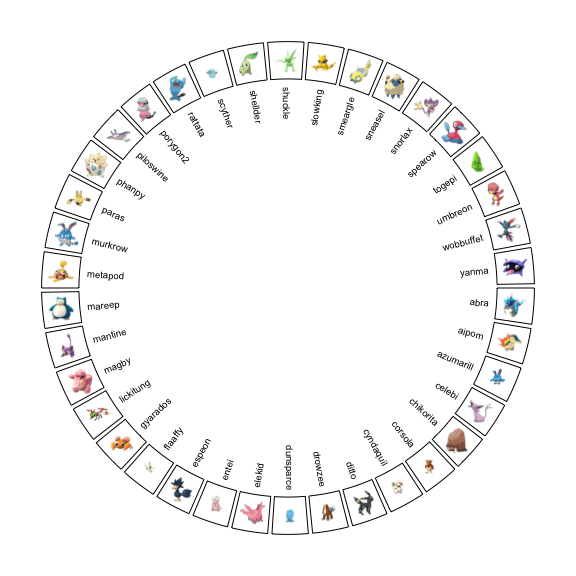
\includegraphics{02-circlize-layout_files/figure-latex/circular-pokemon-1} 

}

\caption{Add raster image to the circular plot.}\label{fig:circular-pokemon}
\end{figure}

\begin{Shaded}
\begin{Highlighting}[]
\KeywordTok{circos.clear}\NormalTok{()}
\end{Highlighting}
\end{Shaded}

In \textbf{circlize} package, there is a \texttt{circos.raster()}
function which directly adds raster images. It is introduced in Section
\ref{raster-image}.

\subsection{The convert functions}\label{convert-functions}

For the functions in \textbf{circlize} package, they needs arguments
which are lengths measured either in the canvas coordinate or in the
data coordinate. E.g. \texttt{track.height} argument in
\texttt{circos.track()} corresponds to percent of radius of the unit
circle. \textbf{circlize} package is built in the R base graphic system
which is not straightforward to define a length with absolute units
(e.g.~a line of length 2 cm). To solve this problem, \textbf{circlize}
provides three functions which convert absolute units to the canvas
coordinate or the data coordinate accordingly.

\texttt{convert\_length()} converts absolute units to the canvas
coordinate. Since the aspect ratio for canvas coordinate is always set
to 1, it doesn't matter whether to convert units in the x direction or
in the y direction. The usage of \texttt{convert\_length()} is
straightforward, supported units are \texttt{mm}, \texttt{cm} and
\texttt{inches}. If users want to convert a string height or width to
the canvas coordinate, directly use \texttt{strheight()} or
\texttt{strwidth()} functions.

\begin{Shaded}
\begin{Highlighting}[]
\KeywordTok{convert_length}\NormalTok{(}\DecValTok{2}\NormalTok{, }\StringTok{"mm"}\NormalTok{)}
\end{Highlighting}
\end{Shaded}

Since \texttt{convert\_length()} is mostly used to define heights on the
radical direction, e.g.~track height or height of track margins, the
function has another name \texttt{convert\_height()}, or the short name
\texttt{uh()} (stands for \emph{unit height}).

\texttt{convert\_x()} and \texttt{convert\_y()}, or the short version
\texttt{ux()} and \texttt{uy()} (\emph{unit x} and \emph{unit y}),
convert absolute units to the data coordinate. By default, the
conversion is applied in the ``current'' cell, but it can still be used
in other cells by specifying \texttt{sector.index} and
\texttt{track.index} arguments. Since the width of the cell is not
identical from the top to the bottom in the cell, for
\texttt{convert\_x()} or \texttt{ux()} function, the position on y
direction where the convert is applied needs to be specified. By default
it is at the middle point on y-axis.

Following plot (Figure \ref{fig:unit-convert}) is an example of setting
absolute units.

\begin{Shaded}
\begin{Highlighting}[]
\NormalTok{fa =}\StringTok{ }\NormalTok{letters[}\DecValTok{1}\OperatorTok{:}\DecValTok{10}\NormalTok{]}
\KeywordTok{circos.par}\NormalTok{(}\DataTypeTok{cell.padding =} \KeywordTok{c}\NormalTok{(}\DecValTok{0}\NormalTok{, }\DecValTok{0}\NormalTok{, }\DecValTok{0}\NormalTok{, }\DecValTok{0}\NormalTok{), }\DataTypeTok{track.margin =} \KeywordTok{c}\NormalTok{(}\DecValTok{0}\NormalTok{, }\DecValTok{0}\NormalTok{))}
\KeywordTok{circos.initialize}\NormalTok{(fa, }\DataTypeTok{xlim =} \KeywordTok{cbind}\NormalTok{(}\KeywordTok{rep}\NormalTok{(}\DecValTok{0}\NormalTok{, }\DecValTok{10}\NormalTok{), }\KeywordTok{runif}\NormalTok{(}\DecValTok{10}\NormalTok{, }\FloatTok{0.5}\NormalTok{, }\FloatTok{1.5}\NormalTok{)))}
\KeywordTok{circos.track}\NormalTok{(}\DataTypeTok{ylim =} \KeywordTok{c}\NormalTok{(}\DecValTok{0}\NormalTok{, }\DecValTok{1}\NormalTok{), }\DataTypeTok{track.height =} \KeywordTok{uh}\NormalTok{(}\DecValTok{5}\NormalTok{, }\StringTok{"mm"}\NormalTok{),}
    \DataTypeTok{panel.fun =} \ControlFlowTok{function}\NormalTok{(x, y) \{}
        \KeywordTok{circos.lines}\NormalTok{(}\KeywordTok{c}\NormalTok{(}\DecValTok{0}\NormalTok{, }\DecValTok{0} \OperatorTok{+}\StringTok{ }\KeywordTok{ux}\NormalTok{(}\DecValTok{5}\NormalTok{, }\StringTok{"mm"}\NormalTok{)), }\KeywordTok{c}\NormalTok{(}\FloatTok{0.5}\NormalTok{, }\FloatTok{0.5}\NormalTok{), }\DataTypeTok{col =} \StringTok{"blue"}\NormalTok{)}
\NormalTok{    \})}
\KeywordTok{circos.track}\NormalTok{(}\DataTypeTok{ylim =} \KeywordTok{c}\NormalTok{(}\DecValTok{0}\NormalTok{, }\DecValTok{1}\NormalTok{), }\DataTypeTok{track.height =} \KeywordTok{uh}\NormalTok{(}\DecValTok{1}\NormalTok{, }\StringTok{"cm"}\NormalTok{),}
    \DataTypeTok{track.margin =} \KeywordTok{c}\NormalTok{(}\DecValTok{0}\NormalTok{, }\KeywordTok{uh}\NormalTok{(}\DecValTok{2}\NormalTok{, }\StringTok{"mm"}\NormalTok{)),}
    \DataTypeTok{panel.fun =} \ControlFlowTok{function}\NormalTok{(x, y) \{}
\NormalTok{        xcenter =}\StringTok{ }\KeywordTok{get.cell.meta.data}\NormalTok{(}\StringTok{"xcenter"}\NormalTok{)}
        \KeywordTok{circos.lines}\NormalTok{(}\KeywordTok{c}\NormalTok{(xcenter, xcenter), }\KeywordTok{c}\NormalTok{(}\DecValTok{0}\NormalTok{, }\KeywordTok{uy}\NormalTok{(}\DecValTok{1}\NormalTok{, }\StringTok{"cm"}\NormalTok{)), }\DataTypeTok{col =} \StringTok{"red"}\NormalTok{)}
\NormalTok{    \})}
\KeywordTok{circos.track}\NormalTok{(}\DataTypeTok{ylim =} \KeywordTok{c}\NormalTok{(}\DecValTok{0}\NormalTok{, }\DecValTok{1}\NormalTok{), }\DataTypeTok{track.height =} \KeywordTok{uh}\NormalTok{(}\DecValTok{1}\NormalTok{, }\StringTok{"inches"}\NormalTok{),}
    \DataTypeTok{track.margin =} \KeywordTok{c}\NormalTok{(}\DecValTok{0}\NormalTok{, }\KeywordTok{uh}\NormalTok{(}\DecValTok{5}\NormalTok{, }\StringTok{"mm"}\NormalTok{)),}
    \DataTypeTok{panel.fun =} \ControlFlowTok{function}\NormalTok{(x, y) \{}
\NormalTok{        line_length_on_x =}\StringTok{ }\KeywordTok{ux}\NormalTok{(}\DecValTok{1}\OperatorTok{*}\KeywordTok{sqrt}\NormalTok{(}\DecValTok{2}\NormalTok{)}\OperatorTok{/}\DecValTok{2}\NormalTok{, }\StringTok{"cm"}\NormalTok{)}
\NormalTok{        line_length_on_y =}\StringTok{ }\KeywordTok{uy}\NormalTok{(}\DecValTok{1}\OperatorTok{*}\KeywordTok{sqrt}\NormalTok{(}\DecValTok{2}\NormalTok{)}\OperatorTok{/}\DecValTok{2}\NormalTok{, }\StringTok{"cm"}\NormalTok{)}
        \KeywordTok{circos.lines}\NormalTok{(}\KeywordTok{c}\NormalTok{(}\DecValTok{0}\NormalTok{, line_length_on_x), }\KeywordTok{c}\NormalTok{(}\DecValTok{0}\NormalTok{, line_length_on_y), }\DataTypeTok{col =} \StringTok{"orange"}\NormalTok{)}
\NormalTok{    \})}
\end{Highlighting}
\end{Shaded}

\begin{figure}

{\centering 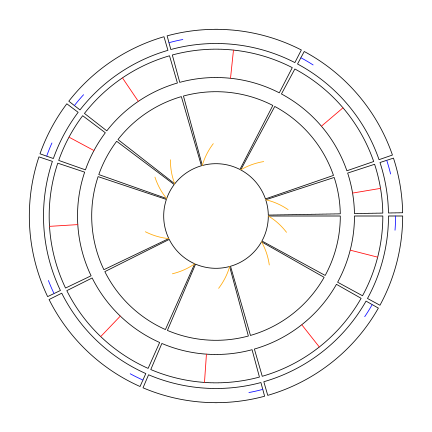
\includegraphics{02-circlize-layout_files/figure-latex/unit-convert-1} 

}

\caption{Setting absolute units}\label{fig:unit-convert}
\end{figure}

\begin{Shaded}
\begin{Highlighting}[]
\KeywordTok{circos.clear}\NormalTok{()}
\end{Highlighting}
\end{Shaded}

\subsection{\texorpdfstring{\texttt{circos.info()} and
\texttt{circos.clear()}}{circos.info() and circos.clear()}}\label{circos-info-and-circos-clear}

You can get basic information of your current circular plot by
\texttt{circos.info()}. The function can be called at any time.

\begin{Shaded}
\begin{Highlighting}[]
\NormalTok{factors =}\StringTok{ }\NormalTok{letters[}\DecValTok{1}\OperatorTok{:}\DecValTok{3}\NormalTok{]}
\KeywordTok{circos.initialize}\NormalTok{(}\DataTypeTok{factors =}\NormalTok{ factors, }\DataTypeTok{xlim =} \KeywordTok{c}\NormalTok{(}\DecValTok{1}\NormalTok{, }\DecValTok{2}\NormalTok{))}
\KeywordTok{circos.info}\NormalTok{()}
\end{Highlighting}
\end{Shaded}

\begin{verbatim}
## All your sectors:
## [1] "a" "b" "c"
## 
## No track has been created
\end{verbatim}

\begin{Shaded}
\begin{Highlighting}[]
\KeywordTok{circos.track}\NormalTok{(}\DataTypeTok{ylim =} \KeywordTok{c}\NormalTok{(}\DecValTok{0}\NormalTok{, }\DecValTok{1}\NormalTok{))}
\KeywordTok{circos.info}\NormalTok{(}\DataTypeTok{sector.index =} \StringTok{"a"}\NormalTok{, }\DataTypeTok{track.index =} \DecValTok{1}\NormalTok{)}
\end{Highlighting}
\end{Shaded}

\begin{verbatim}
## sector index: 'a'
## track index: 1
## xlim: [1, 2]
## ylim: [0, 1]
## cell.xlim: [0.991453, 2.008547]
## cell.ylim: [-0.1, 1.1]
## xplot (degree): [0, 241]
## yplot (radius): [0.79, 0.99]
## track.margin: c(0.01, 0.01)
## cell.padding: c(0.02, 1, 0.02, 1)
## 
## Your current sector.index is c
## Your current track.index is 1
\end{verbatim}

\begin{Shaded}
\begin{Highlighting}[]
\KeywordTok{circos.clear}\NormalTok{()}
\end{Highlighting}
\end{Shaded}

It can also add labels to all cells by
\texttt{circos.info(plot\ =\ TRUE)}.

You should always call \texttt{circos.clear()} at the end of every
circular plot. There are several parameters for circular plot which can
only be set before \texttt{circos.initialize()}, thus, before you draw
the next circular plot, you need to reset all these parameters.

\chapter{Graphics}\label{graphics}

In this chapter, we will introduce low-level functions that add graphics
to the circle. Usages of most of these functions are similar as normal
graphic functions (e.g. \texttt{points()}, \texttt{lines()}).
Combination use of these functions can generate very complex circular
plots.

All low-level functions accept \texttt{sector.index} and
\texttt{track.index} arguments which indicate which cell the graphics
are added in. By default the graphics are added in the ``current''
sector and ``current'' track, so it is recommended to use them directly
inside \texttt{panel.fun} function. However, they can also be used in
other places with explicitly specifying sector and track index.
Following code shows an example of using \texttt{ciros.points()}.

\begin{Shaded}
\begin{Highlighting}[]
\KeywordTok{circos.track}\NormalTok{(..., }\DataTypeTok{panel.fun =} \ControlFlowTok{function}\NormalTok{(x, y) \{}
    \KeywordTok{circos.points}\NormalTok{(x, y)}
\NormalTok{\})}
\KeywordTok{circos.points}\NormalTok{(x, y, sector.index, track.index)}
\end{Highlighting}
\end{Shaded}

In this chapter, we will also discuss how to customize links and how to
highlight regions in the circle.

\section{Points}\label{points}

Adding points by \texttt{circos.points()} is similar as
\texttt{points()} function. Possible usage is:

\begin{Shaded}
\begin{Highlighting}[]
\KeywordTok{circos.points}\NormalTok{(x, y)}
\KeywordTok{circos.points}\NormalTok{(x, y, sector.index, track.index)}
\KeywordTok{circos.points}\NormalTok{(x, y, pch, col, cex)}
\end{Highlighting}
\end{Shaded}

There is a companion function \texttt{circos.trackPoints()} which adds
points to all sectors in a same track simultaneously. The input of
\texttt{circos.trackPoints()} must contain a vector of categorical
factors, a vector of x values and a vector of y values. X values and y
values are split by the categorical variable and corresponding subset of
x and y values are internally sent to \texttt{circos.points()}.
\texttt{circos.trackPoints()} adds points to the ``current'' track by
default which is the most recently created track. Other tracks can also
be selected by explictly setting \texttt{track.index} argument.

\begin{Shaded}
\begin{Highlighting}[]
\KeywordTok{circos.track}\NormalTok{(...)}
\KeywordTok{circos.trackPoints}\NormalTok{(fa, x, y)}
\end{Highlighting}
\end{Shaded}

\texttt{circos.trackPoints()} is simply implemented by
\texttt{circos.points()} with a \texttt{for} loop. However, it is more
recommended to directly use \texttt{circos.points()} and
\texttt{panel.fun} which provides great more flexibility. Actually
following code is identical to above code.

\begin{Shaded}
\begin{Highlighting}[]
\KeywordTok{circos.track}\NormalTok{(fa, x, y, }\DataTypeTok{panel.fun =} \ControlFlowTok{function}\NormalTok{(x, y) \{}
    \KeywordTok{circos.points}\NormalTok{(x, y)}
\NormalTok{\})}
\end{Highlighting}
\end{Shaded}

Other low-level functions also have their companion
\texttt{circos.track*()} function. The usage is same as
\texttt{circos.trackPoints()} and they will not be further discussed in
following sections.

\section{Lines}\label{lines}

Adding lines by \texttt{circos.lines()} is similar as \texttt{lines()}
function. One additional feature is that the areas under or above the
lines can be filled by specifing \texttt{area} argument to
\texttt{TRUE}. Position of the baseline can be set to a pre-defined
string of \texttt{bottom} or \texttt{top}, or a numeric value which is
the position on y-axis. When \texttt{area} is set to \texttt{TRUE},
\texttt{col} controls the filled color and \texttt{border} controls the
color for the borders.

\texttt{baseline} argument is also workable when \texttt{lty} is set to
\texttt{"h"}. Note when \texttt{lty} is set to \texttt{"h"}, graphic
parameters such as \texttt{col} can be set as a vector with same length
as \texttt{x}. Figure \ref{fig:circlize-lines} illustrates supported
\texttt{lty} settings and \texttt{area}/\texttt{baseline} settings.

\begin{figure}

{\centering 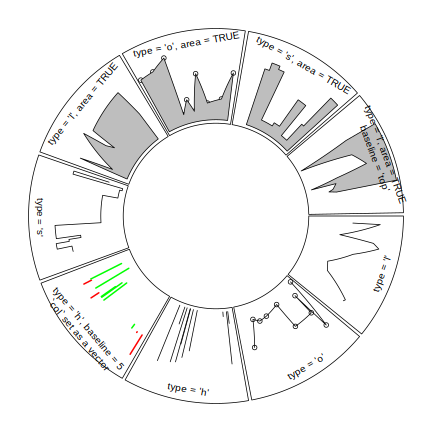
\includegraphics{03-graphics_files/figure-latex/circlize-lines-1} 

}

\caption{Line styles and areas supported in `circos.lines()`}\label{fig:circlize-lines}
\end{figure}

Straight lines are transformed to curves when mapping to the circular
layout (Figure \ref{fig:circlize-linecurve}). Normally, curves are
approximated by a series of segments of straight lines. With more and
shorter segments, there is better approximation, but with larger size if
the figures are generated into e.g.~PDF files, especially for huge
dataset. Default length of segments in \textbf{circlize} is a balance
between the quality and size of the figure. You can set the length of
the unit segment by \texttt{unit.circle.segments} option in
\texttt{circos.par()}. The length of the segment is calculated as the
length of the unit circle (2\(\pi\)) divided by
\texttt{unit.circle.segments}. In some scenarios, actually you don't
need to segment the lines such as radical lines, then you can set
\texttt{straight} argument to \texttt{TRUE} to get rid of unnecessary
segmentations.

\begin{figure}

{\centering 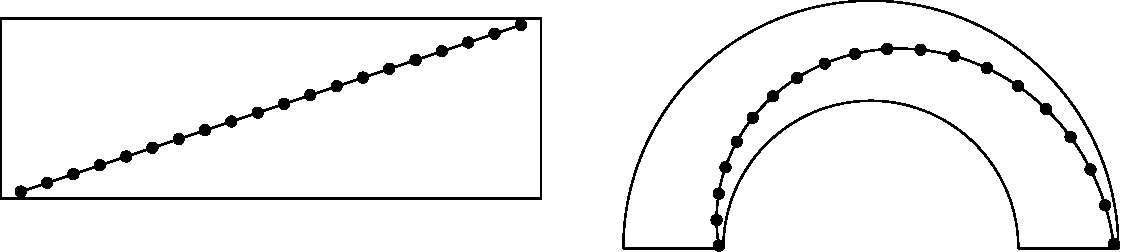
\includegraphics{03-graphics_files/figure-latex/circlize-linecurve-1} 

}

\caption{Transformation of straight lines into curves in the circle.}\label{fig:circlize-linecurve}
\end{figure}

Possible usage for \texttt{circos.lines()} is:

\begin{Shaded}
\begin{Highlighting}[]
\KeywordTok{circos.lines}\NormalTok{(x, y)}
\KeywordTok{circos.lines}\NormalTok{(x, y, sector.index, track.index)}
\KeywordTok{circos.lines}\NormalTok{(x, y, col, lwd, lty, type, straight)}
\KeywordTok{circos.lines}\NormalTok{(x, y, col, area, baseline, border)}
\end{Highlighting}
\end{Shaded}

\section{Segments}\label{segments}

Line segments can be added by \texttt{circos.segments()} function. The
usage is similar as \texttt{segments()}. Radical segments can be added
by setting \texttt{straight} to \texttt{TRUE}.

\begin{Shaded}
\begin{Highlighting}[]
\KeywordTok{circos.segments}\NormalTok{(x0, y0, x1, y1)}
\KeywordTok{circos.segments}\NormalTok{(x0, y0, x1, y1, straight)}
\end{Highlighting}
\end{Shaded}

\section{Text}\label{text}

Adding text by \texttt{circos.text()} is similar as \texttt{text()}
function. Text is added on the plot for human reading, thus, when
putting the text on the circle, the facing of text is very important.
\texttt{circos.text()} supports seven facing options which are
\texttt{inside}, \texttt{outside}, \texttt{clockwise},
\texttt{reverse.clockwise}, \texttt{downward}, \texttt{bending.inside}
and \texttt{bending.outside}. Please note for \texttt{bending.inside}
and \texttt{bending.outside}, currently, single line text is only
supported. If you want to put bended text into two lines, you need to
split text into two lines and add each line by \texttt{circos.text()}
separately. The different facings are illustrated in figure
\ref{fig:circlize-text}.

\begin{figure}

{\centering 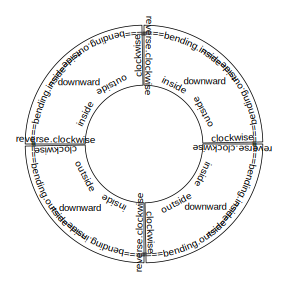
\includegraphics{03-graphics_files/figure-latex/circlize-text-1} 

}

\caption{Text facings.}\label{fig:circlize-text}
\end{figure}

Possible usage for \texttt{circos.text()} is:

\begin{Shaded}
\begin{Highlighting}[]
\KeywordTok{circos.text}\NormalTok{(x, y, labels)}
\KeywordTok{circos.text}\NormalTok{(x, y, labels, sector.index, track.index)}
\KeywordTok{circos.text}\NormalTok{(x, y, labels, facing, niceFacing, adj, cex, col, font)}
\end{Highlighting}
\end{Shaded}

If, e.g., \texttt{facing} is set to \texttt{inside}, text which is on
the bottom half of the circle is still facing to the top and hard to
read. To make text more easy to read and not to hurt readers' neck too
much, \texttt{circos.text()} provides \texttt{niceFacing} option which
automatically adjust text facing according to their positions in the
circle. \texttt{niceFacing} only works for \texttt{facing} value of
\texttt{inside}, \texttt{outside}, \texttt{clockwise},
\texttt{reverse.clockwise}, \texttt{bending.inside} and
\texttt{bending.outside}.

When \texttt{niceFacing} is on, \texttt{adj} is also adjusted according
to the corresponding facings. Figure \ref{fig:circlize-text-easy}
illustrates text positions under different settings of \texttt{adj} and
\texttt{facing}. The red dots are the positions of the texts.

\begin{figure}

{\centering 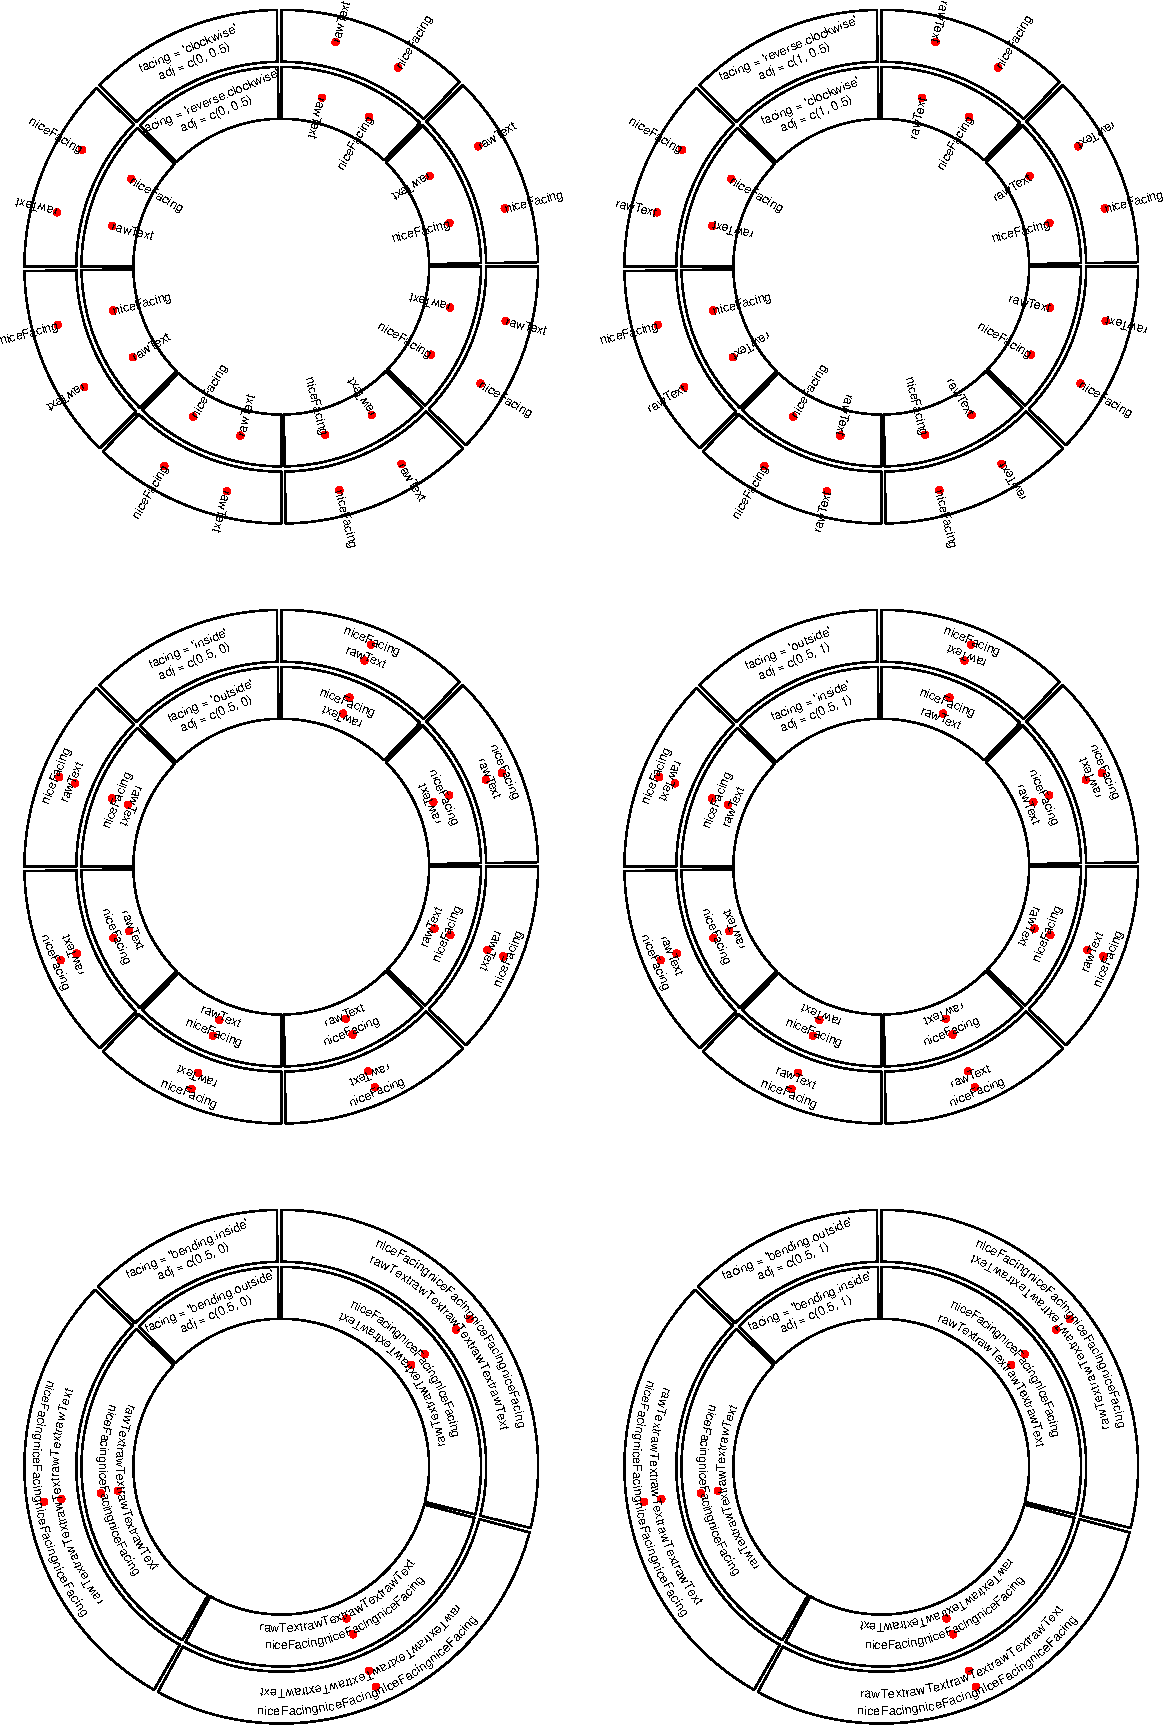
\includegraphics{03-graphics_files/figure-latex/circlize-text-easy-1} 

}

\caption{Human easy text facing.}\label{fig:circlize-text-easy}
\end{figure}

\texttt{adj} is internally passed to \texttt{text()}, thus, it actually
adjusts text positions either horizontally or vertically (in the canvas
coordinate). If the direction of the offset is circular, the offset
value can be set as degrees that the position of the text is adjusted by
wrapping the offset by \texttt{degree()}.

\begin{Shaded}
\begin{Highlighting}[]
\KeywordTok{circos.text}\NormalTok{(x, y, labels, }\DataTypeTok{adj =} \KeywordTok{c}\NormalTok{(}\DecValTok{0}\NormalTok{, }\KeywordTok{degree}\NormalTok{(}\DecValTok{5}\NormalTok{)), }\DataTypeTok{facing =} \StringTok{"clockwise"}\NormalTok{)}
\end{Highlighting}
\end{Shaded}

As \texttt{circos.text()} is applied in the data coordiante, offset can
be directly added to \texttt{x} or/and \texttt{y} as a value measured in
the data coordinate. An absolute offset can be set by using
\texttt{ux()} (in x direction) and \texttt{uy()} (in y direction).

\begin{Shaded}
\begin{Highlighting}[]
\KeywordTok{circos.text}\NormalTok{(x }\OperatorTok{+}\StringTok{ }\KeywordTok{ux}\NormalTok{(}\DecValTok{2}\NormalTok{, }\StringTok{"mm"}\NormalTok{), y }\OperatorTok{+}\StringTok{ }\KeywordTok{uy}\NormalTok{(}\DecValTok{2}\NormalTok{, }\StringTok{"mm"}\NormalTok{), labels)}
\end{Highlighting}
\end{Shaded}

\section{Rectangles and polygons}\label{rectangles}

Theoretically, circular rectangles and polygons are all polygons. If you
imagine the plotting region in a cell as Cartesian coordinate, then
\texttt{circos.rect()} draws rectangles. In the circle, the up and
bottom edge become two arcs. Note this function can be vectorized.

\begin{Shaded}
\begin{Highlighting}[]
\KeywordTok{circos.rect}\NormalTok{(xleft, ybottom, xright, ytop)}
\KeywordTok{circos.rect}\NormalTok{(xleft, ybottom, xright, ytop, sector.index, track.index)}
\KeywordTok{circos.rect}\NormalTok{(xleft, ybottom, xright, ytop, col, border, lty, lwd)}
\end{Highlighting}
\end{Shaded}

\texttt{circos.polygon()} draws a polygon through a series of points in
a cell. Please note the first data point must overlap to the last data
point.

\begin{Shaded}
\begin{Highlighting}[]
\KeywordTok{circos.polygon}\NormalTok{(x, y)}
\KeywordTok{circos.polygon}\NormalTok{(x, y, col, border, lty, lwd)}
\end{Highlighting}
\end{Shaded}

In Figure \ref{fig:circlize-errorline}, the area of standard deviation
of the smoothed line is drawn by \texttt{circos.polygon()}. Source code
can be found in the \textbf{Examples} section of the
\texttt{circos.polygon()} help page.

\begin{figure}

{\centering 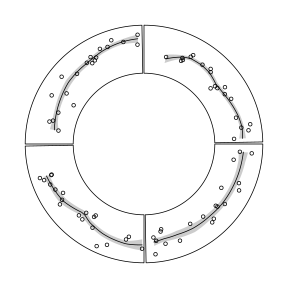
\includegraphics{03-graphics_files/figure-latex/circlize-errorline-1} 

}

\caption{Area of standard deviation of the smoothed line.}\label{fig:circlize-errorline}
\end{figure}

\section{Axes}\label{axes}

Mostly, we only draw x-axes on the circle. \texttt{circos.axis()} or
\texttt{circos.xaxis()} privides options to customize x-axes which are
on the circular direction. It supports basic functionalities as
\texttt{axis()} such as defining the breaks and corresponding labels.
Besides that, the function also supports to put x-axes to a specified
position on y direction, to position the x-axes facing the center of the
circle or outside of the circle, and to customize the axes ticks. The
\texttt{at} and \texttt{labels} arguments can be set to a long vector
that the parts which exceed the maximal value in the corresponding cell
are removed automatically. The facing of labels text can be optimized by
\texttt{labels.niceFacing} (by default it is \texttt{TRUE}).

Figure \ref{fig:circlize-xaxis} illustrates different settings of
x-axes. The explanations are as follows:

\begin{itemize}
\tightlist
\item
  a: Major ticks are calculated automatically, other settings are
  defaults.
\item
  b: Ticks are pointing to inside of the circle, facing of tick labels
  is set to \texttt{outside}.
\item
  c: Position of x-axis is \texttt{bottom} in the cell.
\item
  d: Ticks are pointing to the inside of the circle, facing of tick
  labels is set to \texttt{reverse.clockwise}.
\item
  e: manually set major ticks and also set the position of x-axis.
\item
  f: replace numeric labels to characters, with no minor ticks.
\item
  g: No ticks for both major and minor, facing of tick labels is set to
  \texttt{reverse.clockwise}.
\item
  h: Number of minor ticks between two major ticks is set to 2. Length
  of ticks is longer. Facing of tick labels is set to
  \texttt{clockwise}.
\end{itemize}

\begin{figure}

{\centering 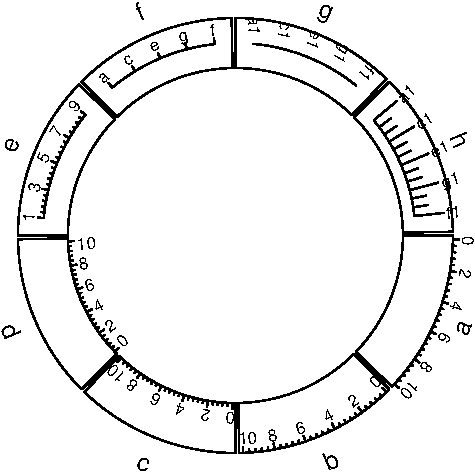
\includegraphics{03-graphics_files/figure-latex/circlize-xaxis-1} 

}

\caption{X-axes}\label{fig:circlize-xaxis}
\end{figure}

As you may notice in the above figure, when the first and last axis
labels exceed data ranges on x-axis in the corresponding cell, their
positions are automatically adjusted to be shifted inwards in the cell.

Possible usage of \texttt{circos.axis()} is as follows. Note \texttt{h}
can be \texttt{bottom}, \texttt{top} or a numeric value.

\begin{Shaded}
\begin{Highlighting}[]
\KeywordTok{circos.axis}\NormalTok{(h)}
\KeywordTok{circos.axis}\NormalTok{(h, sector.index, track.index)}
\KeywordTok{circos.axis}\NormalTok{(h, major.at, labels, major.tick, direction)}
\KeywordTok{circos.axis}\NormalTok{(h, major.at, labels, major.tick, labels.font, labels.cex,}
\NormalTok{            labels.facing, labels.niceFacing)}
\KeywordTok{circos.axis}\NormalTok{(h, major.at, labels, major.tick, minor.ticks,}
\NormalTok{            major.tick.length, lwd)}
\end{Highlighting}
\end{Shaded}

Y-axis is also supported by \texttt{circos.yaxis()}. The usage is
similar as \texttt{circos.axis()} One thing that needs to be note is
users need to manually adjust \texttt{gap.degree} in
\texttt{circos.par()} to make sure there are enough spaces for y-axes.
(Figure \ref{fig:circlize-yaxis})

\begin{Shaded}
\begin{Highlighting}[]
\KeywordTok{circos.yaxis}\NormalTok{(side)}
\KeywordTok{circos.yaxis}\NormalTok{(at, labels, sector.index, track.index)}
\end{Highlighting}
\end{Shaded}

\begin{figure}

{\centering 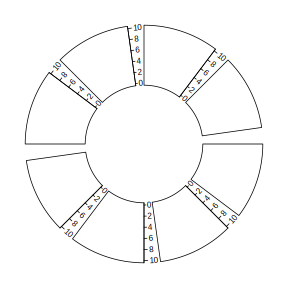
\includegraphics{03-graphics_files/figure-latex/circlize-yaxis-1} 

}

\caption{Y-axes}\label{fig:circlize-yaxis}
\end{figure}

\section{Circular arrows}\label{circular-arrows}

Circular arrows can be used to represent stages in a circle.
\texttt{circos.arrow()} draws circular arrows parallel to the circle.
Since the arrow is always parallel to the circle, on x-direction, the
start and end position of the arrow need to be defined while on the
y-direction, only the position of the center of arrow needs to be
defined. Also \texttt{width} controls the width of the arrow and the
length is defined by \texttt{x2\ -\ x1}. \texttt{arrow.head.width} and
\texttt{arrow.head.length} control the size of the arrow head, and
values are measured in the data coordinate in corresponding cell.
\texttt{tail} controls the shape of the arrow tail. Note for
\texttt{width}, \texttt{arrow.head.width} and
\texttt{arrow.head.length}, the value can be set by \texttt{ux()},
\texttt{uy()} with absolute units. See figure \ref{fig:circular-arrow}.

\begin{Shaded}
\begin{Highlighting}[]
\KeywordTok{circos.initialize}\NormalTok{(letters[}\DecValTok{1}\OperatorTok{:}\DecValTok{4}\NormalTok{], }\DataTypeTok{xlim =} \KeywordTok{c}\NormalTok{(}\DecValTok{0}\NormalTok{, }\DecValTok{1}\NormalTok{))}
\NormalTok{col =}\StringTok{ }\KeywordTok{rand_color}\NormalTok{(}\DecValTok{4}\NormalTok{)}
\NormalTok{tail =}\StringTok{ }\KeywordTok{c}\NormalTok{(}\StringTok{"point"}\NormalTok{, }\StringTok{"normal"}\NormalTok{, }\StringTok{"point"}\NormalTok{, }\StringTok{"normal"}\NormalTok{)}
\KeywordTok{circos.track}\NormalTok{(}\DataTypeTok{ylim =} \KeywordTok{c}\NormalTok{(}\DecValTok{0}\NormalTok{, }\DecValTok{1}\NormalTok{), }\DataTypeTok{panel.fun =} \ControlFlowTok{function}\NormalTok{(x, y) \{}
    \KeywordTok{circos.arrow}\NormalTok{(}\DataTypeTok{x1 =} \DecValTok{0}\NormalTok{, }\DataTypeTok{x2 =} \DecValTok{1}\NormalTok{, }\DataTypeTok{y =} \FloatTok{0.5}\NormalTok{, }\DataTypeTok{width =} \FloatTok{0.4}\NormalTok{, }
        \DataTypeTok{arrow.head.width =} \FloatTok{0.6}\NormalTok{, }\DataTypeTok{arrow.head.length =} \KeywordTok{ux}\NormalTok{(}\DecValTok{1}\NormalTok{, }\StringTok{"cm"}\NormalTok{), }
        \DataTypeTok{col =}\NormalTok{ col[CELL_META}\OperatorTok{$}\NormalTok{sector.numeric.index], }
        \DataTypeTok{tail =}\NormalTok{ tail[CELL_META}\OperatorTok{$}\NormalTok{sector.numeric.index])}
\NormalTok{\}, }\DataTypeTok{bg.border =} \OtherTok{NA}\NormalTok{, }\DataTypeTok{track.height =} \FloatTok{0.4}\NormalTok{)}
\end{Highlighting}
\end{Shaded}

\begin{figure}

{\centering 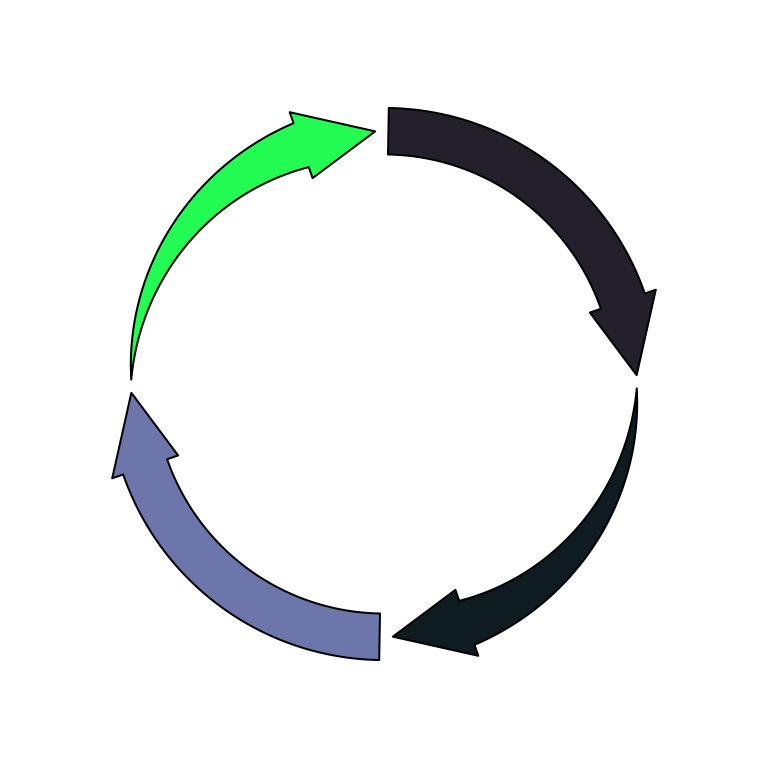
\includegraphics{03-graphics_files/figure-latex/circular-arrow-1} 

}

\caption{Circular arrows.}\label{fig:circular-arrow}
\end{figure}

\begin{Shaded}
\begin{Highlighting}[]
\KeywordTok{circos.clear}\NormalTok{()}
\end{Highlighting}
\end{Shaded}

Circular arrows are useful to visualize events which happen in circular
style, such as different phases in cell cycle. Following example code
visualizes four phases in cell cycle where the width of sectors
correspond to the hours in each phase (figure \ref{fig:cell-cycle}).
Also circular arrows can be used to visualize genes in circular genome
where the arrows represent the orientation of the gene, such as
\href{https://en.wikipedia.org/wiki/Mitochondrial_DNA}{mitochondrial
genome} or \href{https://en.wikipedia.org/wiki/Plasmid}{plasmid genome}.

\begin{Shaded}
\begin{Highlighting}[]
\NormalTok{cell_cycle =}\StringTok{ }\KeywordTok{data.frame}\NormalTok{(}\DataTypeTok{phase =} \KeywordTok{factor}\NormalTok{(}\KeywordTok{c}\NormalTok{(}\StringTok{"G1"}\NormalTok{, }\StringTok{"S"}\NormalTok{, }\StringTok{"G2"}\NormalTok{, }\StringTok{"M"}\NormalTok{), }\DataTypeTok{levels =} \KeywordTok{c}\NormalTok{(}\StringTok{"G1"}\NormalTok{, }\StringTok{"S"}\NormalTok{, }\StringTok{"G2"}\NormalTok{, }\StringTok{"M"}\NormalTok{)),}
                        \DataTypeTok{hour =} \KeywordTok{c}\NormalTok{(}\DecValTok{11}\NormalTok{, }\DecValTok{8}\NormalTok{, }\DecValTok{4}\NormalTok{, }\DecValTok{1}\NormalTok{))}
\NormalTok{color =}\StringTok{ }\KeywordTok{c}\NormalTok{(}\StringTok{"#66C2A5"}\NormalTok{, }\StringTok{"#FC8D62"}\NormalTok{, }\StringTok{"#8DA0CB"}\NormalTok{, }\StringTok{"#E78AC3"}\NormalTok{)}
\KeywordTok{circos.par}\NormalTok{(}\DataTypeTok{start.degree =} \DecValTok{90}\NormalTok{)}
\KeywordTok{circos.initialize}\NormalTok{(cell_cycle}\OperatorTok{$}\NormalTok{phase, }\DataTypeTok{xlim =} \KeywordTok{cbind}\NormalTok{(}\KeywordTok{rep}\NormalTok{(}\DecValTok{0}\NormalTok{, }\DecValTok{4}\NormalTok{), cell_cycle}\OperatorTok{$}\NormalTok{hour))}
\KeywordTok{circos.track}\NormalTok{(}\DataTypeTok{ylim =} \KeywordTok{c}\NormalTok{(}\DecValTok{0}\NormalTok{, }\DecValTok{1}\NormalTok{), }\DataTypeTok{panel.fun =} \ControlFlowTok{function}\NormalTok{(x, y) \{}
    \KeywordTok{circos.arrow}\NormalTok{(CELL_META}\OperatorTok{$}\NormalTok{xlim[}\DecValTok{1}\NormalTok{], CELL_META}\OperatorTok{$}\NormalTok{xlim[}\DecValTok{2}\NormalTok{], }
        \DataTypeTok{arrow.head.width =}\NormalTok{ CELL_META}\OperatorTok{$}\NormalTok{yrange}\OperatorTok{*}\FloatTok{0.8}\NormalTok{, }\DataTypeTok{arrow.head.length =} \KeywordTok{ux}\NormalTok{(}\FloatTok{0.5}\NormalTok{, }\StringTok{"cm"}\NormalTok{),}
        \DataTypeTok{col =}\NormalTok{ color[CELL_META}\OperatorTok{$}\NormalTok{sector.numeric.index])}
    \KeywordTok{circos.text}\NormalTok{(CELL_META}\OperatorTok{$}\NormalTok{xcenter, CELL_META}\OperatorTok{$}\NormalTok{ycenter, CELL_META}\OperatorTok{$}\NormalTok{sector.index, }
        \DataTypeTok{facing =} \StringTok{"downward"}\NormalTok{)}
    \KeywordTok{circos.axis}\NormalTok{(}\DataTypeTok{h =} \DecValTok{1}\NormalTok{, }\DataTypeTok{major.at =} \KeywordTok{seq}\NormalTok{(}\DecValTok{0}\NormalTok{, }\KeywordTok{round}\NormalTok{(CELL_META}\OperatorTok{$}\NormalTok{xlim[}\DecValTok{2}\NormalTok{])), }\DataTypeTok{minor.ticks =} \DecValTok{1}\NormalTok{,}
        \DataTypeTok{labels.cex =} \FloatTok{0.6}\NormalTok{)}
\NormalTok{\}, }\DataTypeTok{bg.border =} \OtherTok{NA}\NormalTok{, }\DataTypeTok{track.height =} \FloatTok{0.3}\NormalTok{)}
\end{Highlighting}
\end{Shaded}

\begin{figure}

{\centering 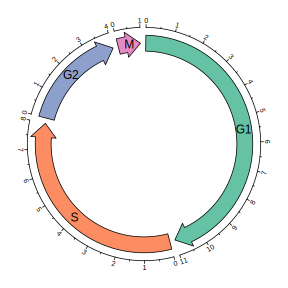
\includegraphics{03-graphics_files/figure-latex/cell-cycle-1} 

}

\caption{Cell cycle.}\label{fig:cell-cycle}
\end{figure}

\begin{Shaded}
\begin{Highlighting}[]
\KeywordTok{circos.clear}\NormalTok{()}
\end{Highlighting}
\end{Shaded}

\section{Raster image}\label{raster-image}

\texttt{circos.raster()} is used to add a raster image at a certain
position in the circle with proper rotation. The first input variable
should be a \texttt{raster} object or an object that can be converted by
\texttt{as.raster()}. Facing of the image is controlled by
\texttt{facing} and \texttt{niceFacing} arguments which are similar as
in \texttt{circos.text()}. When value of \texttt{facing} is one of
\texttt{inside}, \texttt{outside}, \texttt{reverse.clockwise},
\texttt{clockwise} and \texttt{downward}, the size of raster image
should have absolute values which should be specified in the form of
\texttt{number-\ unit} such as \texttt{"20mm"}, \texttt{"1.2cm"} or
\texttt{"0.5inche"}. If only one of \texttt{width} and \texttt{height}
is specified, the other one is automatically calculated by using the
aspect ratio of the original image. Following example shows five types
of facings of the raster image (figure \ref{fig:raster-normal}).

\begin{Shaded}
\begin{Highlighting}[]
\KeywordTok{library}\NormalTok{(png)}
\NormalTok{image =}\StringTok{ }\KeywordTok{system.file}\NormalTok{(}\StringTok{"extdata"}\NormalTok{, }\StringTok{"Rlogo.png"}\NormalTok{, }\DataTypeTok{package =} \StringTok{"circlize"}\NormalTok{)}
\NormalTok{image =}\StringTok{ }\KeywordTok{as.raster}\NormalTok{(}\KeywordTok{readPNG}\NormalTok{(image))}
\KeywordTok{circos.par}\NormalTok{(}\DataTypeTok{start.degree =} \DecValTok{90}\NormalTok{)}
\KeywordTok{circos.initialize}\NormalTok{(letters[}\DecValTok{1}\OperatorTok{:}\DecValTok{5}\NormalTok{], }\DataTypeTok{xlim =} \KeywordTok{c}\NormalTok{(}\DecValTok{0}\NormalTok{, }\DecValTok{1}\NormalTok{))}
\NormalTok{all_facing_options =}\StringTok{ }\KeywordTok{c}\NormalTok{(}\StringTok{"inside"}\NormalTok{, }\StringTok{"outside"}\NormalTok{, }\StringTok{"reverse.clockwise"}\NormalTok{, }\StringTok{"clockwise"}\NormalTok{, }\StringTok{"downward"}\NormalTok{)}
\KeywordTok{circos.track}\NormalTok{(}\DataTypeTok{ylim =} \KeywordTok{c}\NormalTok{(}\DecValTok{0}\NormalTok{, }\DecValTok{1}\NormalTok{), }\DataTypeTok{panel.fun =} \ControlFlowTok{function}\NormalTok{(x, y) \{}
    \KeywordTok{circos.raster}\NormalTok{(image, CELL_META}\OperatorTok{$}\NormalTok{xcenter, CELL_META}\OperatorTok{$}\NormalTok{ycenter, }\DataTypeTok{width =} \StringTok{"1cm"}\NormalTok{, }
        \DataTypeTok{facing =}\NormalTok{ all_facing_options[CELL_META}\OperatorTok{$}\NormalTok{sector.numeric.index])}
    \KeywordTok{circos.text}\NormalTok{(CELL_META}\OperatorTok{$}\NormalTok{xcenter, CELL_META}\OperatorTok{$}\NormalTok{ycenter, }
\NormalTok{        all_facing_options[CELL_META}\OperatorTok{$}\NormalTok{sector.numeric.index],}
        \DataTypeTok{facing =} \StringTok{"inside"}\NormalTok{, }\DataTypeTok{niceFacing =} \OtherTok{TRUE}\NormalTok{)}
\NormalTok{\})}
\end{Highlighting}
\end{Shaded}

\begin{figure}

{\centering 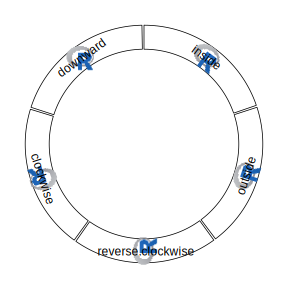
\includegraphics{03-graphics_files/figure-latex/raster-normal-1} 

}

\caption{Five facings of raster image.}\label{fig:raster-normal}
\end{figure}

\begin{Shaded}
\begin{Highlighting}[]
\KeywordTok{circos.clear}\NormalTok{()}
\end{Highlighting}
\end{Shaded}

Also \texttt{facing} can be set to \texttt{bending.inside} and
\texttt{bending.outside} that the image is filled to a circular
rectangle. The strategy is to plot each original pixel as a small
circular rectangle by \texttt{circos.rect()}, thus, the plotting is
quite slow. If the original image is too huge, \texttt{scaling} argument
can be set to reduce the size of the original image.

Following code draws the image of the cover of this book which is a
circular style of
\href{https://en.wikipedia.org/wiki/Keith_Haring}{Keith Haring}'s doodle
(Figure \ref{fig:raster-doodle}). The original source of the plot is
from
\url{http://www.thegreenhead.com/imgs/keith-haring-double-retrospect-worlds-largest-jigsaw-puzzle-2.jpg}.

\begin{Shaded}
\begin{Highlighting}[]
\KeywordTok{load}\NormalTok{(}\KeywordTok{system.file}\NormalTok{(}\StringTok{"extdata"}\NormalTok{, }\StringTok{"doodle.RData"}\NormalTok{, }\DataTypeTok{package =} \StringTok{"circlize"}\NormalTok{))}
\KeywordTok{circos.par}\NormalTok{(}\StringTok{"cell.padding"}\NormalTok{ =}\StringTok{ }\KeywordTok{c}\NormalTok{(}\DecValTok{0}\NormalTok{, }\DecValTok{0}\NormalTok{, }\DecValTok{0}\NormalTok{, }\DecValTok{0}\NormalTok{))}
\KeywordTok{circos.initialize}\NormalTok{(letters[}\DecValTok{1}\OperatorTok{:}\DecValTok{16}\NormalTok{], }\DataTypeTok{xlim =} \KeywordTok{c}\NormalTok{(}\DecValTok{0}\NormalTok{, }\DecValTok{1}\NormalTok{))}
\KeywordTok{circos.track}\NormalTok{(}\DataTypeTok{ylim =} \KeywordTok{c}\NormalTok{(}\DecValTok{0}\NormalTok{, }\DecValTok{1}\NormalTok{), }\DataTypeTok{panel.fun =} \ControlFlowTok{function}\NormalTok{(x, y) \{}
\NormalTok{    img =}\StringTok{ }\NormalTok{img_list[[CELL_META}\OperatorTok{$}\NormalTok{sector.numeric.index]]}
    \KeywordTok{circos.raster}\NormalTok{(img, CELL_META}\OperatorTok{$}\NormalTok{xcenter, CELL_META}\OperatorTok{$}\NormalTok{ycenter, }
        \DataTypeTok{width =}\NormalTok{ CELL_META}\OperatorTok{$}\NormalTok{xrange, }\DataTypeTok{height =}\NormalTok{ CELL_META}\OperatorTok{$}\NormalTok{yrange, }
        \DataTypeTok{facing =} \StringTok{"bending.inside"}\NormalTok{)}
\NormalTok{\}, }\DataTypeTok{track.height =} \FloatTok{0.25}\NormalTok{, }\DataTypeTok{bg.border =} \OtherTok{NA}\NormalTok{)}
\KeywordTok{circos.track}\NormalTok{(}\DataTypeTok{ylim =} \KeywordTok{c}\NormalTok{(}\DecValTok{0}\NormalTok{, }\DecValTok{1}\NormalTok{), }\DataTypeTok{panel.fun =} \ControlFlowTok{function}\NormalTok{(x, y) \{}
\NormalTok{    img =}\StringTok{ }\NormalTok{img_list[[CELL_META}\OperatorTok{$}\NormalTok{sector.numeric.index }\OperatorTok{+}\StringTok{ }\DecValTok{16}\NormalTok{]]}
    \KeywordTok{circos.raster}\NormalTok{(img, CELL_META}\OperatorTok{$}\NormalTok{xcenter, CELL_META}\OperatorTok{$}\NormalTok{ycenter, }
        \DataTypeTok{width =}\NormalTok{ CELL_META}\OperatorTok{$}\NormalTok{xrange, }\DataTypeTok{height =}\NormalTok{ CELL_META}\OperatorTok{$}\NormalTok{yrange, }
        \DataTypeTok{facing =} \StringTok{"bending.inside"}\NormalTok{)}
\NormalTok{\}, }\DataTypeTok{track.height =} \FloatTok{0.25}\NormalTok{, }\DataTypeTok{bg.border =} \OtherTok{NA}\NormalTok{)}
\KeywordTok{circos.clear}\NormalTok{()}
\end{Highlighting}
\end{Shaded}

\begin{figure}

{\centering 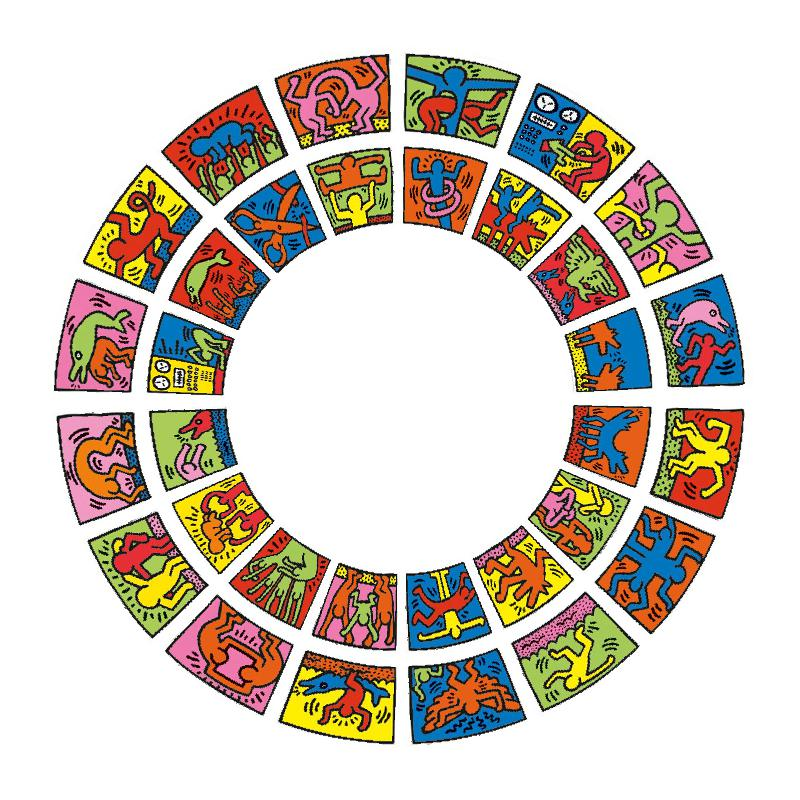
\includegraphics[width=11.11in]{images/doodle} 

}

\caption{Fill raster image to the cell.}\label{fig:raster-doodle}
\end{figure}

\section{Links}\label{links}

Links or ribbons are important part for the circular visualization. They
are used to represent relations or interactions between sectors. In
\textbf{circlize}, \texttt{circos.link()} draws links between single
points and intervals. There are four mandatory arguments which are index
for the first sector, positions on the first sector, index for the
second sector and positions on the second sector. If the positions on
the two sectors are all single points, the link represents as a line. If
the positions on the two sectors are intervals, the link represents as a
robbon (Figure \ref{fig:link-example}). Possible usage for
\texttt{circos.link()} is as follows.

\begin{Shaded}
\begin{Highlighting}[]
\KeywordTok{circos.link}\NormalTok{(sector.index1, }\DecValTok{0}\NormalTok{, sector.index2, }\DecValTok{0}\NormalTok{)}
\KeywordTok{circos.link}\NormalTok{(sector.index1, }\KeywordTok{c}\NormalTok{(}\DecValTok{0}\NormalTok{, }\DecValTok{1}\NormalTok{), sector.index2, }\DecValTok{0}\NormalTok{)}
\KeywordTok{circos.link}\NormalTok{(sector.index1, }\KeywordTok{c}\NormalTok{(}\DecValTok{0}\NormalTok{, }\DecValTok{1}\NormalTok{), sector.index2, }\KeywordTok{c}\NormalTok{(}\DecValTok{1}\NormalTok{, }\DecValTok{2}\NormalTok{))}
\KeywordTok{circos.link}\NormalTok{(sector.index1, }\KeywordTok{c}\NormalTok{(}\DecValTok{0}\NormalTok{, }\DecValTok{1}\NormalTok{), sector.index2, }\DecValTok{0}\NormalTok{, col, lwd, lty, border)}
\end{Highlighting}
\end{Shaded}

\begin{figure}

{\centering 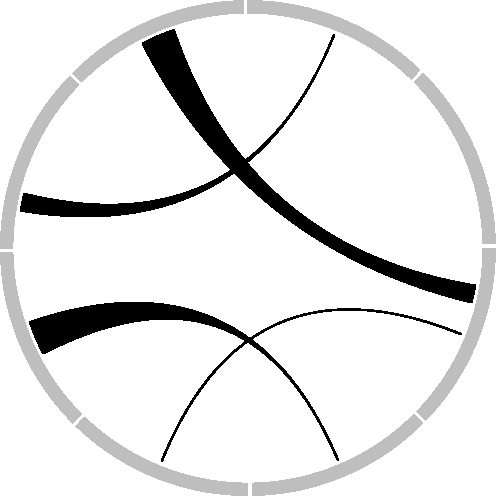
\includegraphics{03-graphics_files/figure-latex/link-example-1} 

}

\caption{Different types of links.}\label{fig:link-example}
\end{figure}

The position of link end is controlled by \texttt{rou}. By default, it
is the bottom of the most inside track and normally, you don't need to
care about this setting. The two ends of the link are located in a same
circle by default. The positions of two ends can be adjusted with
different values for \texttt{rou1} and \texttt{rou2} arguments. See
Figure \ref{fig:link-end}.

\begin{Shaded}
\begin{Highlighting}[]
\KeywordTok{circos.link}\NormalTok{(sector.index1, }\DecValTok{0}\NormalTok{, sector.index2, }\DecValTok{0}\NormalTok{, rou)}
\KeywordTok{circos.link}\NormalTok{(sector.index1, }\DecValTok{0}\NormalTok{, sector.index2, }\DecValTok{0}\NormalTok{, rou1, rou2)}
\end{Highlighting}
\end{Shaded}

\begin{figure}

{\centering 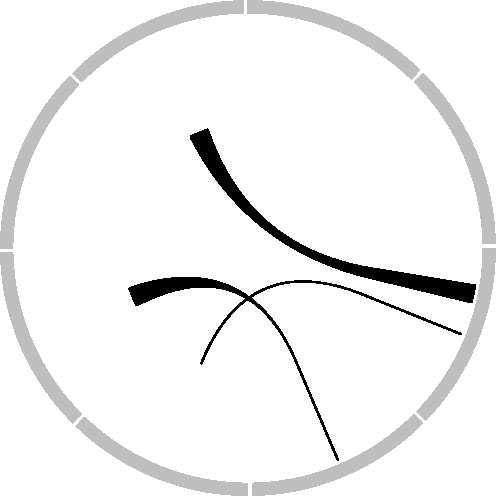
\includegraphics{03-graphics_files/figure-latex/link-end-1} 

}

\caption{Positions of link ends.}\label{fig:link-end}
\end{figure}

The height of the link is controlled by \texttt{h} argument. In most
cases, you don't need to care about the value of \texttt{h} because they
are internally calculated based on the width of each link. However, when
the link represents as a ribbon (i.e.~link from point to interval or
from interval to interval), It can not always ensure that one border is
always below or above the other, which means, in some extreme cases, the
two borders are intersected and the link would be messed up. It happens
especially when position of the two ends are too close or the width of
one end is extremely large while the width of the other end is too
small. In that case, users can manually set height of the top and bottom
border by \texttt{h} and \texttt{h2} (Figure \ref{fig:link-height}).

\begin{Shaded}
\begin{Highlighting}[]
\KeywordTok{circos.link}\NormalTok{(sector.index1, }\DecValTok{0}\NormalTok{, sector.index2, }\DecValTok{0}\NormalTok{, h)}
\KeywordTok{circos.link}\NormalTok{(sector.index1, }\DecValTok{0}\NormalTok{, sector.index2, }\DecValTok{0}\NormalTok{, h, h2)}
\end{Highlighting}
\end{Shaded}

\begin{figure}

{\centering 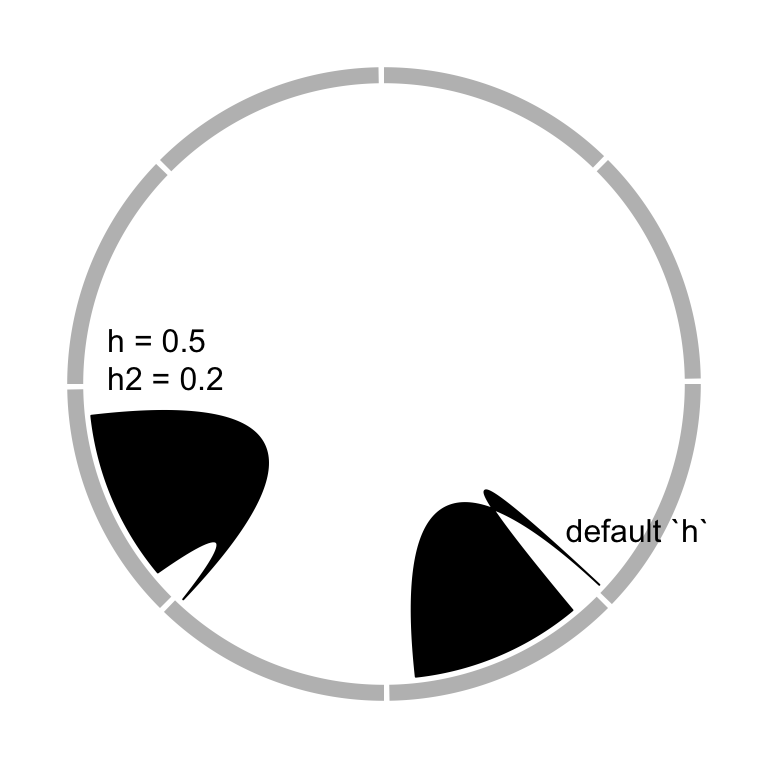
\includegraphics{03-graphics_files/figure-latex/link-height-1} 

}

\caption{Adjust link heights.}\label{fig:link-height}
\end{figure}

When there are many links, the height of all links can be systematically
adjusted by \texttt{h.ratio} (Figure \ref{fig:link-ratio}). The value is
between 0 and 1.

\begin{figure}

{\centering 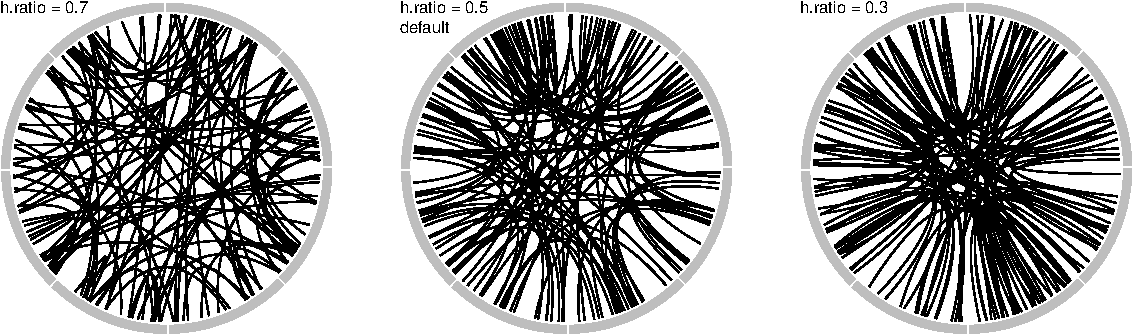
\includegraphics{03-graphics_files/figure-latex/link-ratio-1} 

}

\caption{Adjust link heights by `h.ratio`.}\label{fig:link-ratio}
\end{figure}

The border of link (if it is a ribbon) or the link itself (if it is a
line) is in fact a quadratic Bezier curve, thus you can control the
shape of the link by \texttt{w} and \texttt{w2} (\texttt{w2} controls
the shape of bottom border). See Figure \ref{fig:link-shape} for
examples. For more explanation of \texttt{w}, please refer to
\url{http://en.wikipedia.org/wiki/B\%C3\%A9zier_curve\#Rational_B.C3.A9zier_curves}.

\begin{Shaded}
\begin{Highlighting}[]
\KeywordTok{circos.link}\NormalTok{(sector.index1, }\DecValTok{0}\NormalTok{, sector.index2, }\DecValTok{0}\NormalTok{, w)}
\KeywordTok{circos.link}\NormalTok{(sector.index1, }\DecValTok{0}\NormalTok{, sector.index2, }\DecValTok{0}\NormalTok{, w, w2)}
\end{Highlighting}
\end{Shaded}

\begin{figure}

{\centering 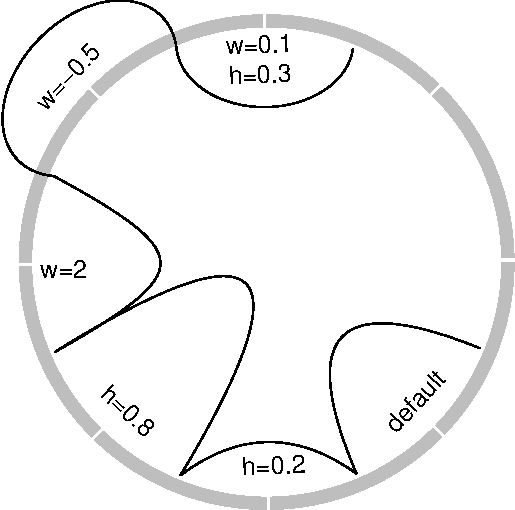
\includegraphics{03-graphics_files/figure-latex/link-shape-1} 

}

\caption{Different link shapes.}\label{fig:link-shape}
\end{figure}

When the links represent as ribbons and the two ends overlap, the links
will be de-generated as a `hill' (Figure \ref{fig:link-hill}).

\begin{figure}

{\centering 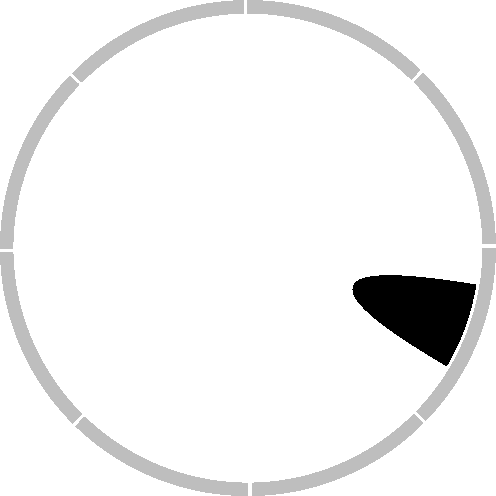
\includegraphics{03-graphics_files/figure-latex/link-hill-1} 

}

\caption{Link as a hill.}\label{fig:link-hill}
\end{figure}

Links can have arrows to represent the directions. The
\texttt{directional} argument controls how to add arrows. A value of
\texttt{0} means there is no direction, \texttt{1} means the direction
is from end 1 to end 2, \texttt{-1} means the direction is from end 2 to
end 1, and \texttt{2} means bi-direction. If the link represents as a
ribbon, a line with arrow will be added in the center of the link to
represent directions. See Figure \ref{fig:link-arrow}.

Type of arrows is controlled by \texttt{arr.type} argument and it is
actually passed to \texttt{Arrowhead()} defined in \textbf{shape}
package. Besides the arrow types supported in \textbf{shape} package,
there is an additional arrow type \texttt{big.arrow} which turns the
robbon into a big arrow (Figure \ref{fig:link-arrow}).

Unequal height of the link ends can also represent directions which we
will discuss more with the \texttt{chordDiagram()} function.

\begin{Shaded}
\begin{Highlighting}[]
\KeywordTok{circos.link}\NormalTok{(sector.index1, }\DecValTok{0}\NormalTok{, sector.index2, }\DecValTok{0}\NormalTok{, }\DataTypeTok{directional =} \DecValTok{1}\NormalTok{)}
\KeywordTok{circos.link}\NormalTok{(sector.index1, }\KeywordTok{c}\NormalTok{(}\DecValTok{0}\NormalTok{, }\DecValTok{1}\NormalTok{), sector.index2, }\KeywordTok{c}\NormalTok{(}\DecValTok{0}\NormalTok{, }\DecValTok{1}\NormalTok{), }\DataTypeTok{directional =} \OperatorTok{-}\DecValTok{1}\NormalTok{)}
\end{Highlighting}
\end{Shaded}

\begin{figure}

{\centering 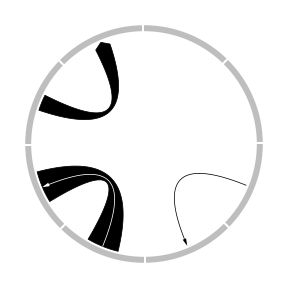
\includegraphics{03-graphics_files/figure-latex/link-arrow-1} 

}

\caption{Link with arrows.}\label{fig:link-arrow}
\end{figure}

\section{Highlight sectors and
tracks}\label{highlight-sectors-and-tracks}

\texttt{draw.sector()} draws sectors, rings or their parts. This
function is useful if you want to highlight some parts of your circular
plot. it needs arguments of the position of circle center (by default
\texttt{c(0,\ 0)}), the start degree and the end degree for sectors, and
radius for two edges (or one edge) which are up or bottom borders.
\texttt{draw.sector()} is independent from the circular plot.

Possible usage of \texttt{draw.sector()} is as follows.

\begin{Shaded}
\begin{Highlighting}[]
\KeywordTok{draw.sector}\NormalTok{(start.degree, end.degree, rou1)}
\KeywordTok{draw.sector}\NormalTok{(start.degree, end.degree, rou1, rou2, center)}
\KeywordTok{draw.sector}\NormalTok{(start.degree, end.degree, rou1, rou2, center, col, border, lwd, lty)}
\end{Highlighting}
\end{Shaded}

Directions from \texttt{start.degree} and \texttt{end.degree} is
important for drawing sectors. By default, it is clock wise.

\begin{Shaded}
\begin{Highlighting}[]
\KeywordTok{draw.sector}\NormalTok{(start.degree, end.degree, }\DataTypeTok{clock.wise =} \OtherTok{FALSE}\NormalTok{)}
\end{Highlighting}
\end{Shaded}

Following code shows examples of \texttt{draw.sector()} (Figure
\ref{fig:draw-sector-general}).

\begin{Shaded}
\begin{Highlighting}[]
\KeywordTok{par}\NormalTok{(}\DataTypeTok{mar =} \KeywordTok{c}\NormalTok{(}\DecValTok{1}\NormalTok{, }\DecValTok{1}\NormalTok{, }\DecValTok{1}\NormalTok{, }\DecValTok{1}\NormalTok{))}
\KeywordTok{plot}\NormalTok{(}\KeywordTok{c}\NormalTok{(}\OperatorTok{-}\DecValTok{1}\NormalTok{, }\DecValTok{1}\NormalTok{), }\KeywordTok{c}\NormalTok{(}\OperatorTok{-}\DecValTok{1}\NormalTok{, }\DecValTok{1}\NormalTok{), }\DataTypeTok{type =} \StringTok{"n"}\NormalTok{, }\DataTypeTok{axes =} \OtherTok{FALSE}\NormalTok{, }\DataTypeTok{ann =} \OtherTok{FALSE}\NormalTok{, }\DataTypeTok{asp =} \DecValTok{1}\NormalTok{)}
\KeywordTok{draw.sector}\NormalTok{(}\DecValTok{20}\NormalTok{, }\DecValTok{0}\NormalTok{)}
\KeywordTok{draw.sector}\NormalTok{(}\DecValTok{30}\NormalTok{, }\DecValTok{60}\NormalTok{, }\DataTypeTok{rou1 =} \FloatTok{0.8}\NormalTok{, }\DataTypeTok{rou2 =} \FloatTok{0.5}\NormalTok{, }\DataTypeTok{clock.wise =} \OtherTok{FALSE}\NormalTok{, }\DataTypeTok{col =} \StringTok{"#FF000080"}\NormalTok{)}
\KeywordTok{draw.sector}\NormalTok{(}\DecValTok{350}\NormalTok{, }\DecValTok{1000}\NormalTok{, }\DataTypeTok{col =} \StringTok{"#00FF0080"}\NormalTok{, }\DataTypeTok{border =} \OtherTok{NA}\NormalTok{)}
\KeywordTok{draw.sector}\NormalTok{(}\DecValTok{0}\NormalTok{, }\DecValTok{180}\NormalTok{, }\DataTypeTok{rou1 =} \FloatTok{0.25}\NormalTok{, }\DataTypeTok{center =} \KeywordTok{c}\NormalTok{(}\OperatorTok{-}\FloatTok{0.5}\NormalTok{, }\FloatTok{0.5}\NormalTok{), }\DataTypeTok{border =} \DecValTok{2}\NormalTok{, }\DataTypeTok{lwd =} \DecValTok{2}\NormalTok{, }\DataTypeTok{lty =} \DecValTok{2}\NormalTok{)}
\KeywordTok{draw.sector}\NormalTok{(}\DecValTok{0}\NormalTok{, }\DecValTok{360}\NormalTok{, }\DataTypeTok{rou1 =} \FloatTok{0.7}\NormalTok{, }\DataTypeTok{rou2 =} \FloatTok{0.6}\NormalTok{, }\DataTypeTok{col =} \StringTok{"#0000FF80"}\NormalTok{)}
\end{Highlighting}
\end{Shaded}

\begin{figure}

{\centering 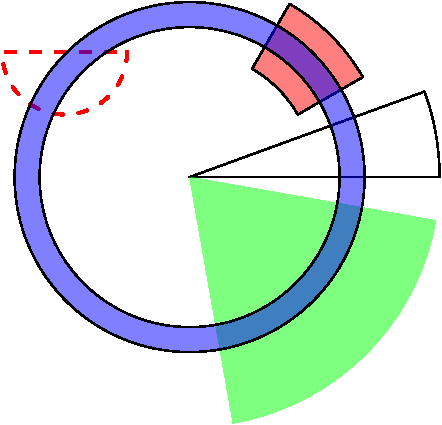
\includegraphics{03-graphics_files/figure-latex/draw-sector-general-1} 

}

\caption{General usage of `draw.sector()`.}\label{fig:draw-sector-general}
\end{figure}

In order to highlight cells in the circular plot, we can use
\texttt{get.cell.meta.data()} to get the information of positions of
cells. E.g. the start degree and end degree can be obtained through
\texttt{cell.start.degree} and \texttt{cell.end.degree}, and the
position of the top border and bottom border can be obtained through
\texttt{cell.top.radius} and \texttt{cell.bottom.radius}. Following code
shows several examples to highlight sectors and tracks.

First we create a circular plot with eight sectors and three tracks.

\begin{Shaded}
\begin{Highlighting}[]
\NormalTok{factors =}\StringTok{ }\NormalTok{letters[}\DecValTok{1}\OperatorTok{:}\DecValTok{8}\NormalTok{]}
\KeywordTok{circos.initialize}\NormalTok{(factors, }\DataTypeTok{xlim =} \KeywordTok{c}\NormalTok{(}\DecValTok{0}\NormalTok{, }\DecValTok{1}\NormalTok{))}
\ControlFlowTok{for}\NormalTok{(i }\ControlFlowTok{in} \DecValTok{1}\OperatorTok{:}\DecValTok{3}\NormalTok{) \{}
    \KeywordTok{circos.track}\NormalTok{(}\DataTypeTok{ylim =} \KeywordTok{c}\NormalTok{(}\DecValTok{0}\NormalTok{, }\DecValTok{1}\NormalTok{))}
\NormalTok{\}}
\KeywordTok{circos.info}\NormalTok{(}\DataTypeTok{plot =} \OtherTok{TRUE}\NormalTok{)}
\end{Highlighting}
\end{Shaded}

If we want to highlight sector a (Figure \ref{fig:circlize-highlight}):

\begin{Shaded}
\begin{Highlighting}[]
\KeywordTok{draw.sector}\NormalTok{(}\KeywordTok{get.cell.meta.data}\NormalTok{(}\StringTok{"cell.start.degree"}\NormalTok{, }\DataTypeTok{sector.index =} \StringTok{"a"}\NormalTok{),}
            \KeywordTok{get.cell.meta.data}\NormalTok{(}\StringTok{"cell.end.degree"}\NormalTok{, }\DataTypeTok{sector.index =} \StringTok{"a"}\NormalTok{),}
            \DataTypeTok{rou1 =} \KeywordTok{get.cell.meta.data}\NormalTok{(}\StringTok{"cell.top.radius"}\NormalTok{, }\DataTypeTok{track.index =} \DecValTok{1}\NormalTok{), }
            \DataTypeTok{col =} \StringTok{"#FF000040"}\NormalTok{)}
\end{Highlighting}
\end{Shaded}

If we want to highlight track 1 (Figure \ref{fig:circlize-highlight}):

\begin{Shaded}
\begin{Highlighting}[]
\KeywordTok{draw.sector}\NormalTok{(}\DecValTok{0}\NormalTok{, }\DecValTok{360}\NormalTok{, }
    \DataTypeTok{rou1 =} \KeywordTok{get.cell.meta.data}\NormalTok{(}\StringTok{"cell.top.radius"}\NormalTok{, }\DataTypeTok{track.index =} \DecValTok{1}\NormalTok{),}
    \DataTypeTok{rou2 =} \KeywordTok{get.cell.meta.data}\NormalTok{(}\StringTok{"cell.bottom.radius"}\NormalTok{, }\DataTypeTok{track.index =} \DecValTok{1}\NormalTok{),}
    \DataTypeTok{col =} \StringTok{"#00FF0040"}\NormalTok{)           }
\end{Highlighting}
\end{Shaded}

If we want to highlight track 2 and 3 in sector e and f (Figure
\ref{fig:circlize-highlight}):

\begin{Shaded}
\begin{Highlighting}[]
\KeywordTok{draw.sector}\NormalTok{(}\KeywordTok{get.cell.meta.data}\NormalTok{(}\StringTok{"cell.start.degree"}\NormalTok{, }\DataTypeTok{sector.index =} \StringTok{"e"}\NormalTok{),}
            \KeywordTok{get.cell.meta.data}\NormalTok{(}\StringTok{"cell.end.degree"}\NormalTok{, }\DataTypeTok{sector.index =} \StringTok{"f"}\NormalTok{),}
            \DataTypeTok{rou1 =} \KeywordTok{get.cell.meta.data}\NormalTok{(}\StringTok{"cell.top.radius"}\NormalTok{, }\DataTypeTok{track.index =} \DecValTok{2}\NormalTok{),}
            \DataTypeTok{rou2 =} \KeywordTok{get.cell.meta.data}\NormalTok{(}\StringTok{"cell.bottom.radius"}\NormalTok{, }\DataTypeTok{track.index =} \DecValTok{3}\NormalTok{),}
            \DataTypeTok{col =} \StringTok{"#0000FF40"}\NormalTok{)}
\end{Highlighting}
\end{Shaded}

If we want to highlight specific regions such as a small region inside
cell \texttt{h:2}, we can use \texttt{circlize()} to calculate the
positions in the polar coordinate. But always keep in mind that x-axis
in the cell are always clock wise. See Figure
\ref{fig:circlize-highlight}.

\begin{Shaded}
\begin{Highlighting}[]
\NormalTok{pos =}\StringTok{ }\KeywordTok{circlize}\NormalTok{(}\KeywordTok{c}\NormalTok{(}\FloatTok{0.2}\NormalTok{, }\FloatTok{0.8}\NormalTok{), }\KeywordTok{c}\NormalTok{(}\FloatTok{0.2}\NormalTok{, }\FloatTok{0.8}\NormalTok{), }\DataTypeTok{sector.index =} \StringTok{"h"}\NormalTok{, }\DataTypeTok{track.index =} \DecValTok{2}\NormalTok{)}
\KeywordTok{draw.sector}\NormalTok{(pos[}\DecValTok{1}\NormalTok{, }\StringTok{"theta"}\NormalTok{], pos[}\DecValTok{2}\NormalTok{, }\StringTok{"theta"}\NormalTok{], pos[}\DecValTok{1}\NormalTok{, }\StringTok{"rou"}\NormalTok{], pos[}\DecValTok{2}\NormalTok{, }\StringTok{"rou"}\NormalTok{], }
    \DataTypeTok{clock.wise =} \OtherTok{TRUE}\NormalTok{, }\DataTypeTok{col =} \StringTok{"#00FFFF40"}\NormalTok{)}
\KeywordTok{circos.clear}\NormalTok{()}
\end{Highlighting}
\end{Shaded}

\begin{figure}

{\centering 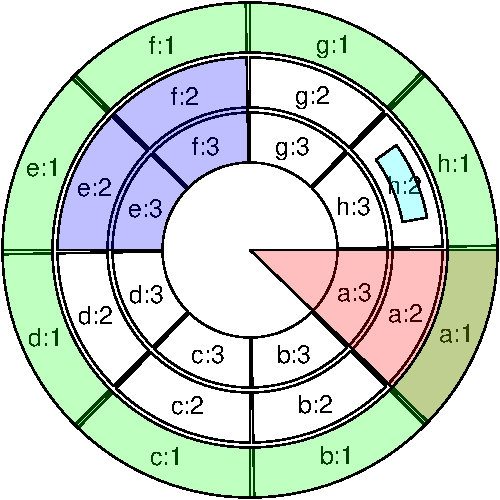
\includegraphics{03-graphics_files/figure-latex/circlize-highlight-1} 

}

\caption{Highlight sectors and tracks.}\label{fig:circlize-highlight}
\end{figure}

If the purpose is to simply highlight complete cells, there is a helper
function \texttt{highlight.sector()} for which you only need to specify
index for sectors and tracks that you want to to highlight. Paddings of
the highligted regions can be set by \texttt{padding} argument which
should contain four values representing ratios of the width or height of
the highlighted region (Figure \ref{fig:circlize-highlight-sector}).

One advantage of \texttt{highlight.sector()} is that it supports to add
text in the highlighted regions. By default, the text is drawn at that
center of the highlighted region. The position on the radical direction
can be set by \texttt{text.vjust} argument either by a numeric value or
a string in form of
\texttt{"2\ inches"\textasciigrave{}\textasciigrave{}\ or}``-1.2cm''`.

\begin{Shaded}
\begin{Highlighting}[]
\NormalTok{factors =}\StringTok{ }\NormalTok{letters[}\DecValTok{1}\OperatorTok{:}\DecValTok{8}\NormalTok{]}
\KeywordTok{circos.initialize}\NormalTok{(factors, }\DataTypeTok{xlim =} \KeywordTok{c}\NormalTok{(}\DecValTok{0}\NormalTok{, }\DecValTok{1}\NormalTok{))}
\ControlFlowTok{for}\NormalTok{(i }\ControlFlowTok{in} \DecValTok{1}\OperatorTok{:}\DecValTok{4}\NormalTok{) \{}
    \KeywordTok{circos.track}\NormalTok{(}\DataTypeTok{ylim =} \KeywordTok{c}\NormalTok{(}\DecValTok{0}\NormalTok{, }\DecValTok{1}\NormalTok{))}
\NormalTok{\}}
\KeywordTok{circos.info}\NormalTok{(}\DataTypeTok{plot =} \OtherTok{TRUE}\NormalTok{)}

\KeywordTok{highlight.sector}\NormalTok{(}\KeywordTok{c}\NormalTok{(}\StringTok{"a"}\NormalTok{, }\StringTok{"h"}\NormalTok{), }\DataTypeTok{track.index =} \DecValTok{1}\NormalTok{, }\DataTypeTok{text =} \StringTok{"a and h belong to a same group"}\NormalTok{,}
    \DataTypeTok{facing =} \StringTok{"bending.inside"}\NormalTok{, }\DataTypeTok{niceFacing =} \OtherTok{TRUE}\NormalTok{, }\DataTypeTok{text.vjust =} \StringTok{"6mm"}\NormalTok{, }\DataTypeTok{cex =} \FloatTok{0.8}\NormalTok{)}
\KeywordTok{highlight.sector}\NormalTok{(}\StringTok{"c"}\NormalTok{, }\DataTypeTok{col =} \StringTok{"#00FF0040"}\NormalTok{)}
\KeywordTok{highlight.sector}\NormalTok{(}\StringTok{"d"}\NormalTok{, }\DataTypeTok{col =} \OtherTok{NA}\NormalTok{, }\DataTypeTok{border =} \StringTok{"red"}\NormalTok{, }\DataTypeTok{lwd =} \DecValTok{2}\NormalTok{)}
\KeywordTok{highlight.sector}\NormalTok{(}\StringTok{"e"}\NormalTok{, }\DataTypeTok{col =} \StringTok{"#0000FF40"}\NormalTok{, }\DataTypeTok{track.index =} \KeywordTok{c}\NormalTok{(}\DecValTok{2}\NormalTok{, }\DecValTok{3}\NormalTok{))}
\KeywordTok{highlight.sector}\NormalTok{(}\KeywordTok{c}\NormalTok{(}\StringTok{"f"}\NormalTok{, }\StringTok{"g"}\NormalTok{), }\DataTypeTok{col =} \OtherTok{NA}\NormalTok{, }\DataTypeTok{border =} \StringTok{"green"}\NormalTok{, }
    \DataTypeTok{lwd =} \DecValTok{2}\NormalTok{, }\DataTypeTok{track.index =} \KeywordTok{c}\NormalTok{(}\DecValTok{2}\NormalTok{, }\DecValTok{3}\NormalTok{), }\DataTypeTok{padding =} \KeywordTok{c}\NormalTok{(}\FloatTok{0.1}\NormalTok{, }\FloatTok{0.1}\NormalTok{, }\FloatTok{0.1}\NormalTok{, }\FloatTok{0.1}\NormalTok{))}
\KeywordTok{highlight.sector}\NormalTok{(factors, }\DataTypeTok{col =} \StringTok{"#FFFF0040"}\NormalTok{, }\DataTypeTok{track.index =} \DecValTok{4}\NormalTok{)}
\end{Highlighting}
\end{Shaded}

\begin{figure}

{\centering 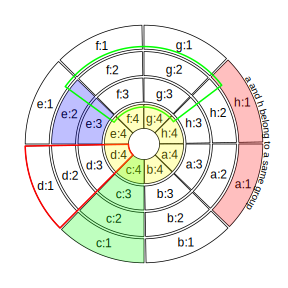
\includegraphics{03-graphics_files/figure-latex/circlize-highlight-sector-1} 

}

\caption{Highlight sectors.}\label{fig:circlize-highlight-sector}
\end{figure}

\begin{Shaded}
\begin{Highlighting}[]
\KeywordTok{circos.clear}\NormalTok{()}
\end{Highlighting}
\end{Shaded}

\section{Work together with the base graphic
system}\label{work-with-base-graphic-system}

\textbf{circlize} is built on the base R graphic system, then, of course
the base graphic functions can be used in combination with circlize
functions. On the other hand, \texttt{circlize()} converts data points
from the data coordinates to the canvas coordinates where the base
graphic function can be directly applied.

Normally, the base functions such as \texttt{title()}, \texttt{text()},
\texttt{legend()} can be used to add extra information on the plot
(Figure \ref{fig:circlize-base}).

Sometimes, when the text or other graphics are far from the circle, you
may set \texttt{par(xpd\ =\ NA)} so that the plotting is not clipped.

\begin{Shaded}
\begin{Highlighting}[]
\NormalTok{factors =}\StringTok{ }\NormalTok{letters[}\DecValTok{1}\OperatorTok{:}\DecValTok{4}\NormalTok{]}
\KeywordTok{circos.initialize}\NormalTok{(}\DataTypeTok{factors =}\NormalTok{ factors, }\DataTypeTok{xlim =} \KeywordTok{c}\NormalTok{(}\DecValTok{0}\NormalTok{, }\DecValTok{1}\NormalTok{))}
\KeywordTok{circos.track}\NormalTok{(}\DataTypeTok{ylim =} \KeywordTok{c}\NormalTok{(}\DecValTok{0}\NormalTok{, }\DecValTok{1}\NormalTok{), }\DataTypeTok{panel.fun =} \ControlFlowTok{function}\NormalTok{(x, y) \{}
    \KeywordTok{circos.points}\NormalTok{(}\DecValTok{1}\OperatorTok{:}\DecValTok{20}\OperatorTok{/}\DecValTok{20}\NormalTok{, }\DecValTok{1}\OperatorTok{:}\DecValTok{20}\OperatorTok{/}\DecValTok{20}\NormalTok{)}
\NormalTok{\})}
\KeywordTok{text}\NormalTok{(}\DecValTok{0}\NormalTok{, }\DecValTok{0}\NormalTok{, }\StringTok{"This is}\CharTok{\textbackslash{}n}\StringTok{the center"}\NormalTok{, }\DataTypeTok{cex =} \FloatTok{1.5}\NormalTok{)}
\KeywordTok{legend}\NormalTok{(}\StringTok{"bottomleft"}\NormalTok{, }\DataTypeTok{pch =} \DecValTok{1}\NormalTok{, }\DataTypeTok{legend =} \StringTok{"This is the legend"}\NormalTok{)}
\KeywordTok{title}\NormalTok{(}\StringTok{"This is the title"}\NormalTok{)}
\end{Highlighting}
\end{Shaded}

\begin{figure}

{\centering 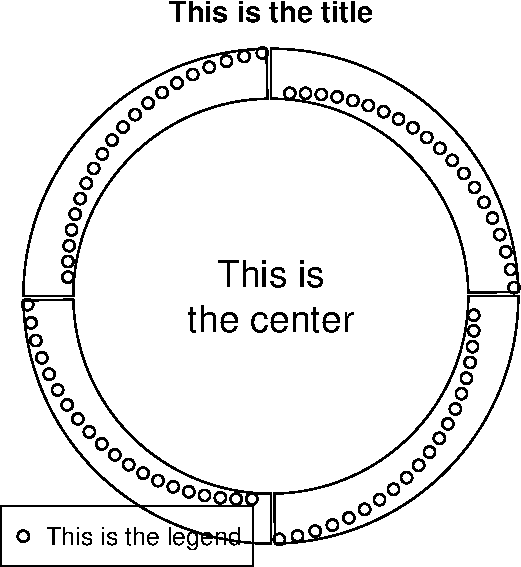
\includegraphics{03-graphics_files/figure-latex/circlize-base-1} 

}

\caption{Work with base graphic functions.}\label{fig:circlize-base}
\end{figure}

\begin{Shaded}
\begin{Highlighting}[]
\KeywordTok{circos.clear}\NormalTok{()}
\end{Highlighting}
\end{Shaded}

\chapter{Legends}\label{legends}

\textbf{circlize} provides complete freedom for users to design their
own graphics by implementing the self-defined function
\texttt{panel.fun}. However one drawback arises that \textbf{circlize}
is completely blind to users' data so that one important thing is
missing for the visualization which is the legend.

Although legends cannot be automatically generated by \textbf{circlize},
by using functionality from other R packages, it is just a few more
lines to really implement it. Here I will demonstrate how to customize
legends and arrange to the circular plot.

As an example, a circular plot which contains two tracks and links
inside the circle is generated. The first track will have a legend that
contains points, the second track will have a legend that contains
lines, and the links correspond to a continuous color mapping. The code
is wrapped into a function so that it can be used repeatedly.

\begin{Shaded}
\begin{Highlighting}[]
\KeywordTok{library}\NormalTok{(circlize)}

\NormalTok{col_fun =}\StringTok{ }\KeywordTok{colorRamp2}\NormalTok{(}\KeywordTok{c}\NormalTok{(}\OperatorTok{-}\DecValTok{2}\NormalTok{, }\DecValTok{0}\NormalTok{, }\DecValTok{2}\NormalTok{), }\KeywordTok{c}\NormalTok{(}\StringTok{"green"}\NormalTok{, }\StringTok{"yellow"}\NormalTok{, }\StringTok{"red"}\NormalTok{))}
\NormalTok{circlize_plot =}\StringTok{ }\ControlFlowTok{function}\NormalTok{() \{}
    \KeywordTok{set.seed}\NormalTok{(}\DecValTok{12345}\NormalTok{)}
\NormalTok{    fa =}\StringTok{ }\NormalTok{letters[}\DecValTok{1}\OperatorTok{:}\DecValTok{10}\NormalTok{]}
    \KeywordTok{circos.initialize}\NormalTok{(fa, }\DataTypeTok{xlim =} \KeywordTok{c}\NormalTok{(}\DecValTok{0}\NormalTok{, }\DecValTok{1}\NormalTok{))}
    \KeywordTok{circos.track}\NormalTok{(}\DataTypeTok{ylim =} \KeywordTok{c}\NormalTok{(}\DecValTok{0}\NormalTok{, }\DecValTok{1}\NormalTok{), }\DataTypeTok{panel.fun =} \ControlFlowTok{function}\NormalTok{(x, y) \{}
        \KeywordTok{circos.points}\NormalTok{(}\KeywordTok{runif}\NormalTok{(}\DecValTok{20}\NormalTok{), }\KeywordTok{runif}\NormalTok{(}\DecValTok{20}\NormalTok{), }\DataTypeTok{cex =} \FloatTok{0.5}\NormalTok{, }\DataTypeTok{pch =} \DecValTok{16}\NormalTok{, }\DataTypeTok{col =} \DecValTok{2}\NormalTok{)}
        \KeywordTok{circos.points}\NormalTok{(}\KeywordTok{runif}\NormalTok{(}\DecValTok{20}\NormalTok{), }\KeywordTok{runif}\NormalTok{(}\DecValTok{20}\NormalTok{), }\DataTypeTok{cex =} \FloatTok{0.5}\NormalTok{, }\DataTypeTok{pch =} \DecValTok{16}\NormalTok{, }\DataTypeTok{col =} \DecValTok{3}\NormalTok{)}
\NormalTok{    \})}
    \KeywordTok{circos.track}\NormalTok{(}\DataTypeTok{ylim =} \KeywordTok{c}\NormalTok{(}\DecValTok{0}\NormalTok{, }\DecValTok{1}\NormalTok{), }\DataTypeTok{panel.fun =} \ControlFlowTok{function}\NormalTok{(x, y) \{}
        \KeywordTok{circos.lines}\NormalTok{(}\KeywordTok{sort}\NormalTok{(}\KeywordTok{runif}\NormalTok{(}\DecValTok{20}\NormalTok{)), }\KeywordTok{runif}\NormalTok{(}\DecValTok{20}\NormalTok{), }\DataTypeTok{col =} \DecValTok{4}\NormalTok{)}
        \KeywordTok{circos.lines}\NormalTok{(}\KeywordTok{sort}\NormalTok{(}\KeywordTok{runif}\NormalTok{(}\DecValTok{20}\NormalTok{)), }\KeywordTok{runif}\NormalTok{(}\DecValTok{20}\NormalTok{), }\DataTypeTok{col =} \DecValTok{5}\NormalTok{)}
\NormalTok{    \})}

    \ControlFlowTok{for}\NormalTok{(i }\ControlFlowTok{in} \DecValTok{1}\OperatorTok{:}\DecValTok{10}\NormalTok{) \{}
        \KeywordTok{circos.link}\NormalTok{(}\KeywordTok{sample}\NormalTok{(fa, }\DecValTok{1}\NormalTok{), }\KeywordTok{sort}\NormalTok{(}\KeywordTok{runif}\NormalTok{(}\DecValTok{10}\NormalTok{))[}\DecValTok{1}\OperatorTok{:}\DecValTok{2}\NormalTok{], }
                    \KeywordTok{sample}\NormalTok{(fa, }\DecValTok{1}\NormalTok{), }\KeywordTok{sort}\NormalTok{(}\KeywordTok{runif}\NormalTok{(}\DecValTok{10}\NormalTok{))[}\DecValTok{1}\OperatorTok{:}\DecValTok{2}\NormalTok{],}
                    \DataTypeTok{col =} \KeywordTok{add_transparency}\NormalTok{(}\KeywordTok{col_fun}\NormalTok{(}\KeywordTok{rnorm}\NormalTok{(}\DecValTok{1}\NormalTok{))))}
\NormalTok{    \}}
    \KeywordTok{circos.clear}\NormalTok{()}
\NormalTok{\}}
\end{Highlighting}
\end{Shaded}

In \textbf{ComplexHeatmap} package with version higher than 1.99.0,
there is a \texttt{Legend()} function which customizes legends with
various styles. In following code, legends for the two tracks and links
are constructed. In the end the three legends are packed vertically by
\texttt{packLegend()}. For more detailed usage of \texttt{Legend()} and
\texttt{packLegend()}, please refer to their help pages.

\begin{Shaded}
\begin{Highlighting}[]
\KeywordTok{library}\NormalTok{(ComplexHeatmap)}
\CommentTok{# discrete}
\NormalTok{lgd_points =}\StringTok{ }\KeywordTok{Legend}\NormalTok{(}\DataTypeTok{at =} \KeywordTok{c}\NormalTok{(}\StringTok{"label1"}\NormalTok{, }\StringTok{"label2"}\NormalTok{), }\DataTypeTok{type =} \StringTok{"points"}\NormalTok{, }
    \DataTypeTok{legend_gp =} \KeywordTok{gpar}\NormalTok{(}\DataTypeTok{col =} \DecValTok{2}\OperatorTok{:}\DecValTok{3}\NormalTok{), }\DataTypeTok{title_position =} \StringTok{"topleft"}\NormalTok{, }
    \DataTypeTok{title =} \StringTok{"Track1"}\NormalTok{)}
\CommentTok{# discrete}
\NormalTok{lgd_lines =}\StringTok{ }\KeywordTok{Legend}\NormalTok{(}\DataTypeTok{at =} \KeywordTok{c}\NormalTok{(}\StringTok{"label3"}\NormalTok{, }\StringTok{"label4"}\NormalTok{), }\DataTypeTok{type =} \StringTok{"lines"}\NormalTok{, }
    \DataTypeTok{legend_gp =} \KeywordTok{gpar}\NormalTok{(}\DataTypeTok{col =} \DecValTok{4}\OperatorTok{:}\DecValTok{5}\NormalTok{, }\DataTypeTok{lwd =} \DecValTok{2}\NormalTok{), }\DataTypeTok{title_position =} \StringTok{"topleft"}\NormalTok{, }
    \DataTypeTok{title =} \StringTok{"Track2"}\NormalTok{)}
\CommentTok{# continuous}
\NormalTok{lgd_links =}\StringTok{ }\KeywordTok{Legend}\NormalTok{(}\DataTypeTok{at =} \KeywordTok{c}\NormalTok{(}\OperatorTok{-}\DecValTok{2}\NormalTok{, }\OperatorTok{-}\DecValTok{1}\NormalTok{, }\DecValTok{0}\NormalTok{, }\DecValTok{1}\NormalTok{, }\DecValTok{2}\NormalTok{), }\DataTypeTok{col_fun =}\NormalTok{ col_fun, }
    \DataTypeTok{title_position =} \StringTok{"topleft"}\NormalTok{, }\DataTypeTok{title =} \StringTok{"Links"}\NormalTok{)}

\NormalTok{lgd_list_vertical =}\StringTok{ }\KeywordTok{packLegend}\NormalTok{(lgd_points, lgd_lines, lgd_links)}
\NormalTok{lgd_list_vertical}
\end{Highlighting}
\end{Shaded}

\begin{verbatim}
## A pack of 3 legends
\end{verbatim}

\texttt{lgd\_points}, \texttt{lgd\_lines}, \texttt{lgd\_links} and
\texttt{lgd\_list\_vertical} are all \texttt{grob} objects (graphical
objects) defined by \textbf{grid} package, which you can think as boxes
which contain all graphical elements for legends and they can be added
to the plot by \texttt{grid.draw()}.

\textbf{circlize} is implemented in the base graphic system while
\textbf{ComplexHeatmap} is implemented by \textbf{grid} graphic system.
However, these two systems can be mixed somehow. We can directly add
grid graphics to the base graphics. (Actually they are two independent
layers but drawn on a same graphic device.)

\begin{Shaded}
\begin{Highlighting}[]
\KeywordTok{circlize_plot}\NormalTok{()}
\CommentTok{# next the grid graphics are added directly to the plot}
\CommentTok{# where circlize has created.}

\KeywordTok{draw}\NormalTok{(lgd_list_vertical, }\DataTypeTok{x =} \KeywordTok{unit}\NormalTok{(}\DecValTok{4}\NormalTok{, }\StringTok{"mm"}\NormalTok{), }\DataTypeTok{y =} \KeywordTok{unit}\NormalTok{(}\DecValTok{4}\NormalTok{, }\StringTok{"mm"}\NormalTok{), }\DataTypeTok{just =} \KeywordTok{c}\NormalTok{(}\StringTok{"left"}\NormalTok{, }\StringTok{"bottom"}\NormalTok{))}
\end{Highlighting}
\end{Shaded}

\begin{figure}

{\centering 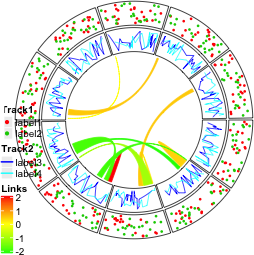
\includegraphics{04-legends_files/figure-latex/directly-add-1} 

}

\caption{Directly add grid graphics.}\label{fig:directly-add}
\end{figure}

In Figure \ref{fig:directly-add}, the whole image region corresponds to
the circular plot and the legend layer is drawn just on top of it.
Actually you can see that one big problem is when there are many legends
that the size for the legends is too big, they may overap to the circle.
One solution is to split the legends into several parts and add each
part to different corners in the plot (Figure \ref{fig:two-legends}).

\begin{Shaded}
\begin{Highlighting}[]
\NormalTok{lgd_list_vertical2 =}\StringTok{ }\KeywordTok{packLegend}\NormalTok{(lgd_points, lgd_lines)}
\KeywordTok{circlize_plot}\NormalTok{()}
\CommentTok{# next the grid graphics are added directly to the plot}
\CommentTok{# where circlize has created.}
\KeywordTok{draw}\NormalTok{(lgd_list_vertical2, }\DataTypeTok{x =} \KeywordTok{unit}\NormalTok{(}\DecValTok{4}\NormalTok{, }\StringTok{"mm"}\NormalTok{), }\DataTypeTok{y =} \KeywordTok{unit}\NormalTok{(}\DecValTok{4}\NormalTok{, }\StringTok{"mm"}\NormalTok{), }\DataTypeTok{just =} \KeywordTok{c}\NormalTok{(}\StringTok{"left"}\NormalTok{, }\StringTok{"bottom"}\NormalTok{))}
\KeywordTok{draw}\NormalTok{(lgd_links, }\DataTypeTok{x =} \KeywordTok{unit}\NormalTok{(}\DecValTok{1}\NormalTok{, }\StringTok{"npc"}\NormalTok{) }\OperatorTok{-}\StringTok{ }\KeywordTok{unit}\NormalTok{(}\DecValTok{2}\NormalTok{, }\StringTok{"mm"}\NormalTok{), }\DataTypeTok{y =} \KeywordTok{unit}\NormalTok{(}\DecValTok{4}\NormalTok{, }\StringTok{"mm"}\NormalTok{), }
    \DataTypeTok{just =} \KeywordTok{c}\NormalTok{(}\StringTok{"right"}\NormalTok{, }\StringTok{"bottom"}\NormalTok{))}
\end{Highlighting}
\end{Shaded}

\begin{figure}

{\centering 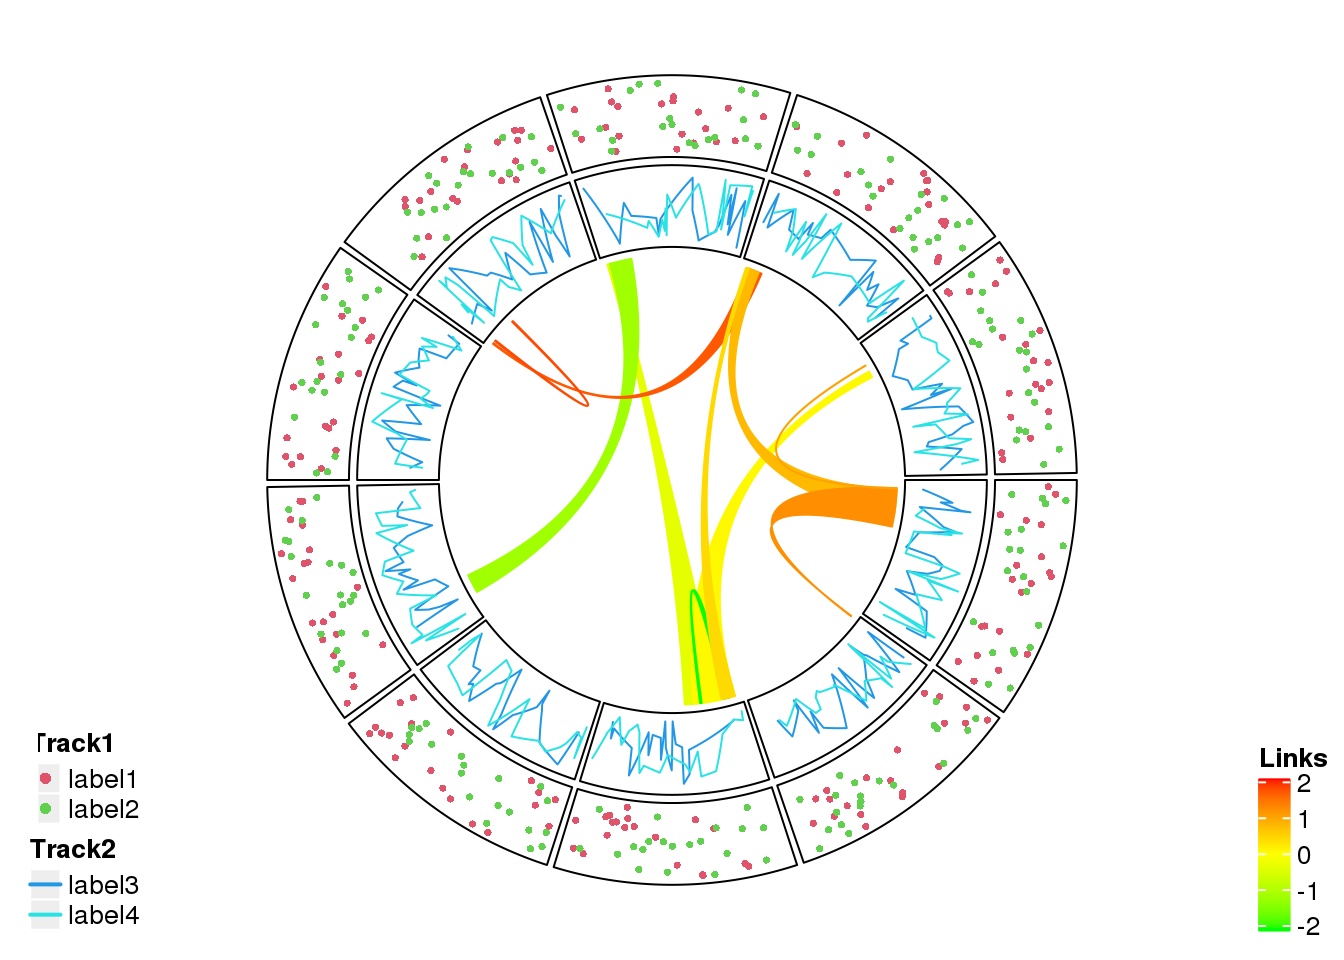
\includegraphics{04-legends_files/figure-latex/two-legends-1} 

}

\caption{Split into two legends.}\label{fig:two-legends}
\end{figure}

Still it can not solve the problem and sometimes it even makes the plot
so messed up. One better way is to split the image region into two parts
where one part only for the circular plot and the other part for
legends.

To mix grid graphics and base graphics, ther are two important packages
to use: the \textbf{grid} package and \textbf{gridBase} package.
\textbf{grid} is the base for making grid graphics as well as arranging
plotting regions (or, \emph{viewports} in \textbf{grid} term), and
\textbf{gridBase} makes it easy to integrate base graphics into grid
system.

Following code is straightforward to understand. Only one line needs to
be noticed: \texttt{par(omi\ =\ gridOMI(),\ new\ =\ TRUE)} that
\texttt{gridOMI()} calculates the outer margins for the base graphics so
that the base graphics can be put at the correct place and
\texttt{new\ =\ TRUE} to ensure the base graphics are added to current
graphic device instead of opening a new one.

Here I use \texttt{plot.new()} to open a new graphic device. In
interactive session, it seems ok if you also use
\texttt{grid.newpage()}, but \texttt{grid.newpage()} gives error when
building a \textbf{knitr} document.

\begin{Shaded}
\begin{Highlighting}[]
\KeywordTok{library}\NormalTok{(gridBase)}
\KeywordTok{plot.new}\NormalTok{()}
\NormalTok{circle_size =}\StringTok{ }\KeywordTok{unit}\NormalTok{(}\DecValTok{1}\NormalTok{, }\StringTok{"snpc"}\NormalTok{) }\CommentTok{# snpc unit gives you a square region}

\KeywordTok{pushViewport}\NormalTok{(}\KeywordTok{viewport}\NormalTok{(}\DataTypeTok{x =} \DecValTok{0}\NormalTok{, }\DataTypeTok{y =} \FloatTok{0.5}\NormalTok{, }\DataTypeTok{width =}\NormalTok{ circle_size, }\DataTypeTok{height =}\NormalTok{ circle_size,}
    \DataTypeTok{just =} \KeywordTok{c}\NormalTok{(}\StringTok{"left"}\NormalTok{, }\StringTok{"center"}\NormalTok{)))}
\KeywordTok{par}\NormalTok{(}\DataTypeTok{omi =} \KeywordTok{gridOMI}\NormalTok{(), }\DataTypeTok{new =} \OtherTok{TRUE}\NormalTok{)}
\KeywordTok{circlize_plot}\NormalTok{()}
\KeywordTok{upViewport}\NormalTok{()}

\KeywordTok{draw}\NormalTok{(lgd_list_vertical, }\DataTypeTok{x =}\NormalTok{ circle_size, }\DataTypeTok{just =} \StringTok{"left"}\NormalTok{)}
\end{Highlighting}
\end{Shaded}

\begin{center}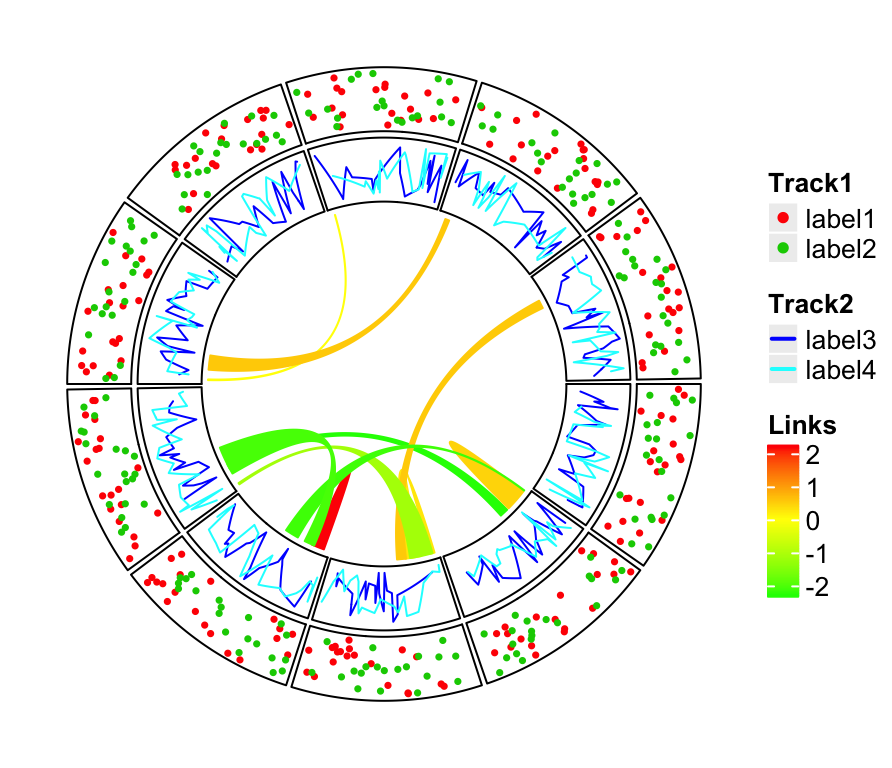
\includegraphics{04-legends_files/figure-latex/right-legend-1} \end{center}

The legends can also be put at the bottom of the circular plot and it is
just a matter how users arrange the grid viewports. In this case, all
legends are changed to horizontal style, and three legends are packed
horizontally as well.

\begin{Shaded}
\begin{Highlighting}[]
\NormalTok{lgd_points =}\StringTok{ }\KeywordTok{Legend}\NormalTok{(}\DataTypeTok{at =} \KeywordTok{c}\NormalTok{(}\StringTok{"label1"}\NormalTok{, }\StringTok{"label2"}\NormalTok{), }\DataTypeTok{type =} \StringTok{"points"}\NormalTok{, }
    \DataTypeTok{legend_gp =} \KeywordTok{gpar}\NormalTok{(}\DataTypeTok{col =} \DecValTok{2}\OperatorTok{:}\DecValTok{3}\NormalTok{), }\DataTypeTok{title_position =} \StringTok{"topleft"}\NormalTok{, }
    \DataTypeTok{title =} \StringTok{"Track1"}\NormalTok{, }\DataTypeTok{nrow =} \DecValTok{1}\NormalTok{)}

\NormalTok{lgd_lines =}\StringTok{ }\KeywordTok{Legend}\NormalTok{(}\DataTypeTok{at =} \KeywordTok{c}\NormalTok{(}\StringTok{"label3"}\NormalTok{, }\StringTok{"label4"}\NormalTok{), }\DataTypeTok{type =} \StringTok{"lines"}\NormalTok{, }
    \DataTypeTok{legend_gp =} \KeywordTok{gpar}\NormalTok{(}\DataTypeTok{col =} \DecValTok{4}\OperatorTok{:}\DecValTok{5}\NormalTok{, }\DataTypeTok{lwd =} \DecValTok{2}\NormalTok{), }\DataTypeTok{title_position =} \StringTok{"topleft"}\NormalTok{, }
    \DataTypeTok{title =} \StringTok{"Track2"}\NormalTok{, }\DataTypeTok{nrow =} \DecValTok{1}\NormalTok{)}

\NormalTok{lgd_links =}\StringTok{ }\KeywordTok{Legend}\NormalTok{(}\DataTypeTok{at =} \KeywordTok{c}\NormalTok{(}\OperatorTok{-}\DecValTok{2}\NormalTok{, }\OperatorTok{-}\DecValTok{1}\NormalTok{, }\DecValTok{0}\NormalTok{, }\DecValTok{1}\NormalTok{, }\DecValTok{2}\NormalTok{), }\DataTypeTok{col_fun =}\NormalTok{ col_fun, }
    \DataTypeTok{title_position =} \StringTok{"topleft"}\NormalTok{, }\DataTypeTok{title =} \StringTok{"Links"}\NormalTok{, }\DataTypeTok{direction =} \StringTok{"horizontal"}\NormalTok{)}

\NormalTok{lgd_list_horizontal =}\StringTok{ }\KeywordTok{packLegend}\NormalTok{(lgd_points, lgd_lines, lgd_links, }
    \DataTypeTok{direction =} \StringTok{"horizontal"}\NormalTok{)}
\end{Highlighting}
\end{Shaded}

Similar code to arrange viewports.

\begin{Shaded}
\begin{Highlighting}[]
\KeywordTok{plot.new}\NormalTok{()}
\KeywordTok{pushViewport}\NormalTok{(}\KeywordTok{viewport}\NormalTok{(}\DataTypeTok{x =} \FloatTok{0.5}\NormalTok{, }\DataTypeTok{y =} \DecValTok{1}\NormalTok{, }\DataTypeTok{width =}\NormalTok{ circle_size, }\DataTypeTok{height =}\NormalTok{ circle_size,}
    \DataTypeTok{just =} \KeywordTok{c}\NormalTok{(}\StringTok{"center"}\NormalTok{, }\StringTok{"top"}\NormalTok{)))}
\KeywordTok{par}\NormalTok{(}\DataTypeTok{omi =} \KeywordTok{gridOMI}\NormalTok{(), }\DataTypeTok{new =} \OtherTok{TRUE}\NormalTok{)}
\KeywordTok{circlize_plot}\NormalTok{()}
\KeywordTok{upViewport}\NormalTok{()}

\KeywordTok{draw}\NormalTok{(lgd_list_horizontal, }\DataTypeTok{y =} \KeywordTok{unit}\NormalTok{(}\DecValTok{1}\NormalTok{, }\StringTok{"npc"}\NormalTok{) }\OperatorTok{-}\StringTok{ }\NormalTok{circle_size, }\DataTypeTok{just =} \StringTok{"top"}\NormalTok{)}
\end{Highlighting}
\end{Shaded}

\begin{center}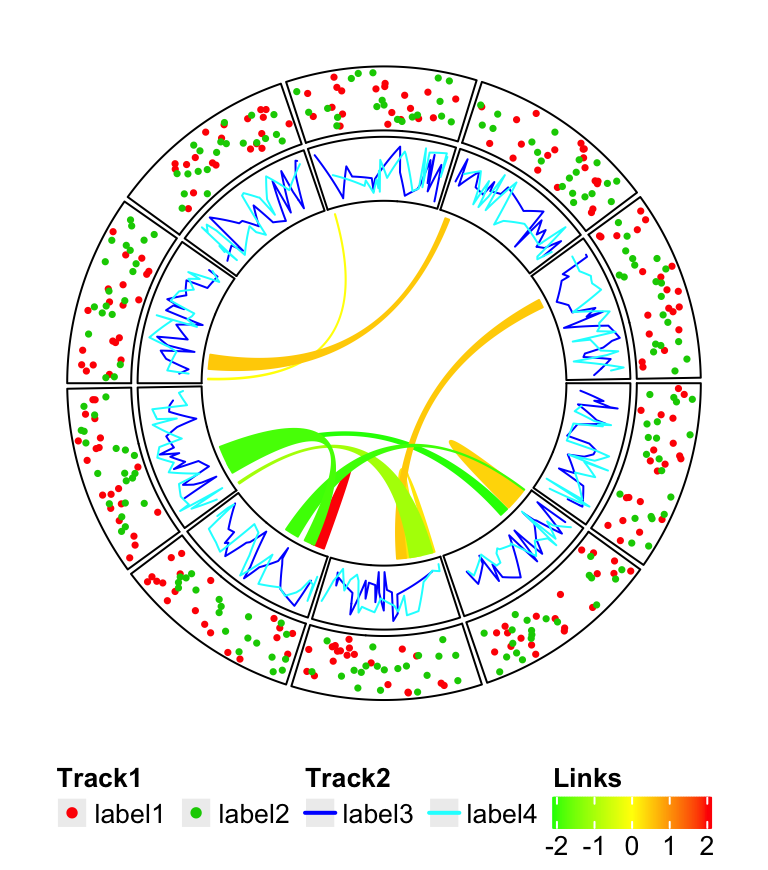
\includegraphics{04-legends_files/figure-latex/bottom-legend-1} \end{center}

\chapter{Implement high-level circular plots}\label{high-level-plots}

In this chapter, we show several examples which combine low-level
graphic functions to construct complicated graphics for specific
purposes.

\section{Circular barplots}\label{circular-barplot}

In the following code, we put all the nine bars in one track and one
sector. You can also put them into 9 tracks, but the code would be very
similar. See Figure \ref{fig:circular-barplot}.

\begin{Shaded}
\begin{Highlighting}[]
\NormalTok{category =}\StringTok{ }\KeywordTok{paste0}\NormalTok{(}\StringTok{"category"}\NormalTok{, }\StringTok{"_"}\NormalTok{, }\DecValTok{1}\OperatorTok{:}\DecValTok{9}\NormalTok{)}
\NormalTok{percent =}\StringTok{ }\KeywordTok{sort}\NormalTok{(}\KeywordTok{sample}\NormalTok{(}\DecValTok{40}\OperatorTok{:}\DecValTok{80}\NormalTok{, }\DecValTok{9}\NormalTok{))}
\NormalTok{color =}\StringTok{ }\KeywordTok{rev}\NormalTok{(}\KeywordTok{rainbow}\NormalTok{(}\KeywordTok{length}\NormalTok{(percent)))}

\KeywordTok{library}\NormalTok{(circlize)}
\KeywordTok{circos.par}\NormalTok{(}\StringTok{"start.degree"}\NormalTok{ =}\StringTok{ }\DecValTok{90}\NormalTok{, }\DataTypeTok{cell.padding =} \KeywordTok{c}\NormalTok{(}\DecValTok{0}\NormalTok{, }\DecValTok{0}\NormalTok{, }\DecValTok{0}\NormalTok{, }\DecValTok{0}\NormalTok{))}
\KeywordTok{circos.initialize}\NormalTok{(}\StringTok{"a"}\NormalTok{, }\DataTypeTok{xlim =} \KeywordTok{c}\NormalTok{(}\DecValTok{0}\NormalTok{, }\DecValTok{100}\NormalTok{)) }\CommentTok{# 'a` just means there is one sector}
\KeywordTok{circos.track}\NormalTok{(}\DataTypeTok{ylim =} \KeywordTok{c}\NormalTok{(}\FloatTok{0.5}\NormalTok{, }\KeywordTok{length}\NormalTok{(percent)}\OperatorTok{+}\FloatTok{0.5}\NormalTok{), }\DataTypeTok{track.height =} \FloatTok{0.8}\NormalTok{, }
    \DataTypeTok{bg.border =} \OtherTok{NA}\NormalTok{, }\DataTypeTok{panel.fun =} \ControlFlowTok{function}\NormalTok{(x, y) \{}
\NormalTok{        xlim =}\StringTok{ }\NormalTok{CELL_META}\OperatorTok{$}\NormalTok{xlim}
        \KeywordTok{circos.segments}\NormalTok{(}\KeywordTok{rep}\NormalTok{(xlim[}\DecValTok{1}\NormalTok{], }\DecValTok{9}\NormalTok{), }\DecValTok{1}\OperatorTok{:}\DecValTok{9}\NormalTok{,}
                        \KeywordTok{rep}\NormalTok{(xlim[}\DecValTok{2}\NormalTok{], }\DecValTok{9}\NormalTok{), }\DecValTok{1}\OperatorTok{:}\DecValTok{9}\NormalTok{,}
                        \DataTypeTok{col =} \StringTok{"#CCCCCC"}\NormalTok{)}
        \KeywordTok{circos.rect}\NormalTok{(}\KeywordTok{rep}\NormalTok{(}\DecValTok{0}\NormalTok{, }\DecValTok{9}\NormalTok{), }\DecValTok{1}\OperatorTok{:}\DecValTok{9} \OperatorTok{-}\StringTok{ }\FloatTok{0.45}\NormalTok{, percent, }\DecValTok{1}\OperatorTok{:}\DecValTok{9} \OperatorTok{+}\StringTok{ }\FloatTok{0.45}\NormalTok{,}
            \DataTypeTok{col =}\NormalTok{ color, }\DataTypeTok{border =} \StringTok{"white"}\NormalTok{)}
        \KeywordTok{circos.text}\NormalTok{(}\KeywordTok{rep}\NormalTok{(xlim[}\DecValTok{1}\NormalTok{], }\DecValTok{9}\NormalTok{), }\DecValTok{1}\OperatorTok{:}\DecValTok{9}\NormalTok{, }
            \KeywordTok{paste}\NormalTok{(category, }\StringTok{" - "}\NormalTok{, percent, }\StringTok{"%"}\NormalTok{), }
            \DataTypeTok{facing =} \StringTok{"downward"}\NormalTok{, }\DataTypeTok{adj =} \KeywordTok{c}\NormalTok{(}\FloatTok{1.05}\NormalTok{, }\FloatTok{0.5}\NormalTok{), }\DataTypeTok{cex =} \FloatTok{0.8}\NormalTok{) }
\NormalTok{        breaks =}\StringTok{ }\KeywordTok{seq}\NormalTok{(}\DecValTok{0}\NormalTok{, }\DecValTok{85}\NormalTok{, }\DataTypeTok{by =} \DecValTok{5}\NormalTok{)}
        \KeywordTok{circos.axis}\NormalTok{(}\DataTypeTok{h =} \StringTok{"top"}\NormalTok{, }\DataTypeTok{major.at =}\NormalTok{ breaks, }\DataTypeTok{labels =} \KeywordTok{paste0}\NormalTok{(breaks, }\StringTok{"%"}\NormalTok{), }
            \DataTypeTok{labels.cex =} \FloatTok{0.6}\NormalTok{)}
\NormalTok{\})}
\end{Highlighting}
\end{Shaded}

\begin{figure}

{\centering 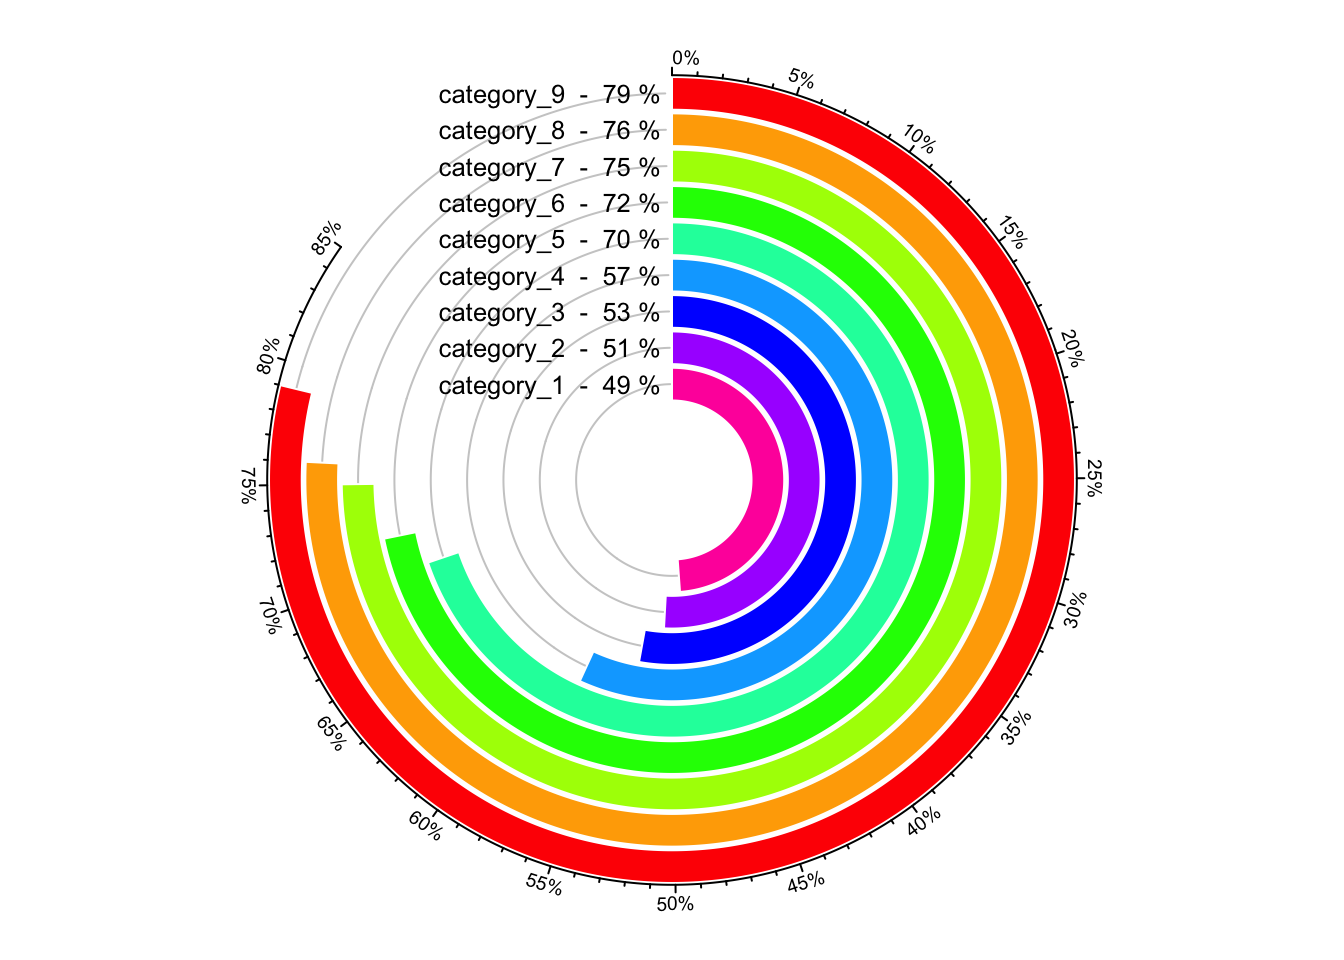
\includegraphics{05-implement-high-level-plots_files/figure-latex/circular-barplot-1} 

}

\caption{A circular barplot.}\label{fig:circular-barplot}
\end{figure}

\begin{Shaded}
\begin{Highlighting}[]
\KeywordTok{circos.clear}\NormalTok{()}
\end{Highlighting}
\end{Shaded}

When adding text by \texttt{circos.text()}, \texttt{adj} is specified to
\texttt{c(1.05,\ 0.5)} which means text is aligned to the right and
there is also offset between the text and the anchor points. We can also
use \texttt{ux()} to set the offset to absolute units. Conversion on x
direction in a circular coordinate is affected by the position on y
axis, here we must set the \texttt{h} argument. Following code can be
used to replace the \texttt{circos.text()} in above example.

\begin{Shaded}
\begin{Highlighting}[]
\KeywordTok{circos.text}\NormalTok{(xlim[}\DecValTok{1}\NormalTok{] }\OperatorTok{-}\StringTok{ }\KeywordTok{ux}\NormalTok{(}\DecValTok{2}\NormalTok{, }\StringTok{"mm"}\NormalTok{, }\DataTypeTok{h =} \DecValTok{1}\OperatorTok{:}\DecValTok{9}\NormalTok{), }\DecValTok{1}\OperatorTok{:}\DecValTok{9}\NormalTok{, }
    \KeywordTok{paste}\NormalTok{(category, }\StringTok{" - "}\NormalTok{, percent, }\StringTok{"%"}\NormalTok{), }
    \DataTypeTok{facing =} \StringTok{"downward"}\NormalTok{, }\DataTypeTok{adj =} \KeywordTok{c}\NormalTok{(}\DecValTok{1}\NormalTok{, }\FloatTok{0.5}\NormalTok{), }\DataTypeTok{cex =} \FloatTok{0.8}\NormalTok{)}
\end{Highlighting}
\end{Shaded}

\section{Histograms}\label{histograms}

\textbf{circlize} ships a \texttt{circos.trackHist()} function which
draws histograms in cells. This function is a high-level function which
caculates data ranges on y axes and creates a new track. The implement
of this function is simple, that it first calculates the histogram in
each cell by \texttt{hist()} function, then draws histogram by using
\texttt{circos.rect()}.

Users can choose to visualize data distributions by density lines by
setting \texttt{draw.density\ =\ TRUE}.

Figure \ref{fig:circular-histograms} shows a histogram track under
default settings, a histogram track with specified \texttt{bin.size} and
a track with density lines. By default, bin size of histogram in each
cell is calculated separatedly and they will be different between cells,
which makes it not consistent to compare. Manually setting
\texttt{bin.size} in all cells to a same value helps to compare the
distributions between cells.

\begin{Shaded}
\begin{Highlighting}[]
\NormalTok{x =}\StringTok{ }\KeywordTok{rnorm}\NormalTok{(}\DecValTok{1600}\NormalTok{)}
\NormalTok{factors =}\StringTok{ }\KeywordTok{sample}\NormalTok{(letters[}\DecValTok{1}\OperatorTok{:}\DecValTok{16}\NormalTok{], }\DecValTok{1600}\NormalTok{, }\DataTypeTok{replace =} \OtherTok{TRUE}\NormalTok{)}
\KeywordTok{circos.initialize}\NormalTok{(}\DataTypeTok{factors =}\NormalTok{ factors, }\DataTypeTok{x =}\NormalTok{ x)}
\KeywordTok{circos.trackHist}\NormalTok{(}\DataTypeTok{factors =}\NormalTok{ factors, }\DataTypeTok{x =}\NormalTok{ x, }\DataTypeTok{col =} \StringTok{"#999999"}\NormalTok{, }
    \DataTypeTok{border =} \StringTok{"#999999"}\NormalTok{)}
\KeywordTok{circos.trackHist}\NormalTok{(}\DataTypeTok{factors =}\NormalTok{ factors, }\DataTypeTok{x =}\NormalTok{ x, }\DataTypeTok{bin.size =} \FloatTok{0.1}\NormalTok{, }
    \DataTypeTok{col =} \StringTok{"#999999"}\NormalTok{, }\DataTypeTok{border =} \StringTok{"#999999"}\NormalTok{)}
\KeywordTok{circos.trackHist}\NormalTok{(}\DataTypeTok{factors =}\NormalTok{ factors, }\DataTypeTok{x =}\NormalTok{ x, }\DataTypeTok{draw.density =} \OtherTok{TRUE}\NormalTok{, }
    \DataTypeTok{col =} \StringTok{"#999999"}\NormalTok{, }\DataTypeTok{border =} \StringTok{"#999999"}\NormalTok{)}
\end{Highlighting}
\end{Shaded}

\begin{figure}

{\centering 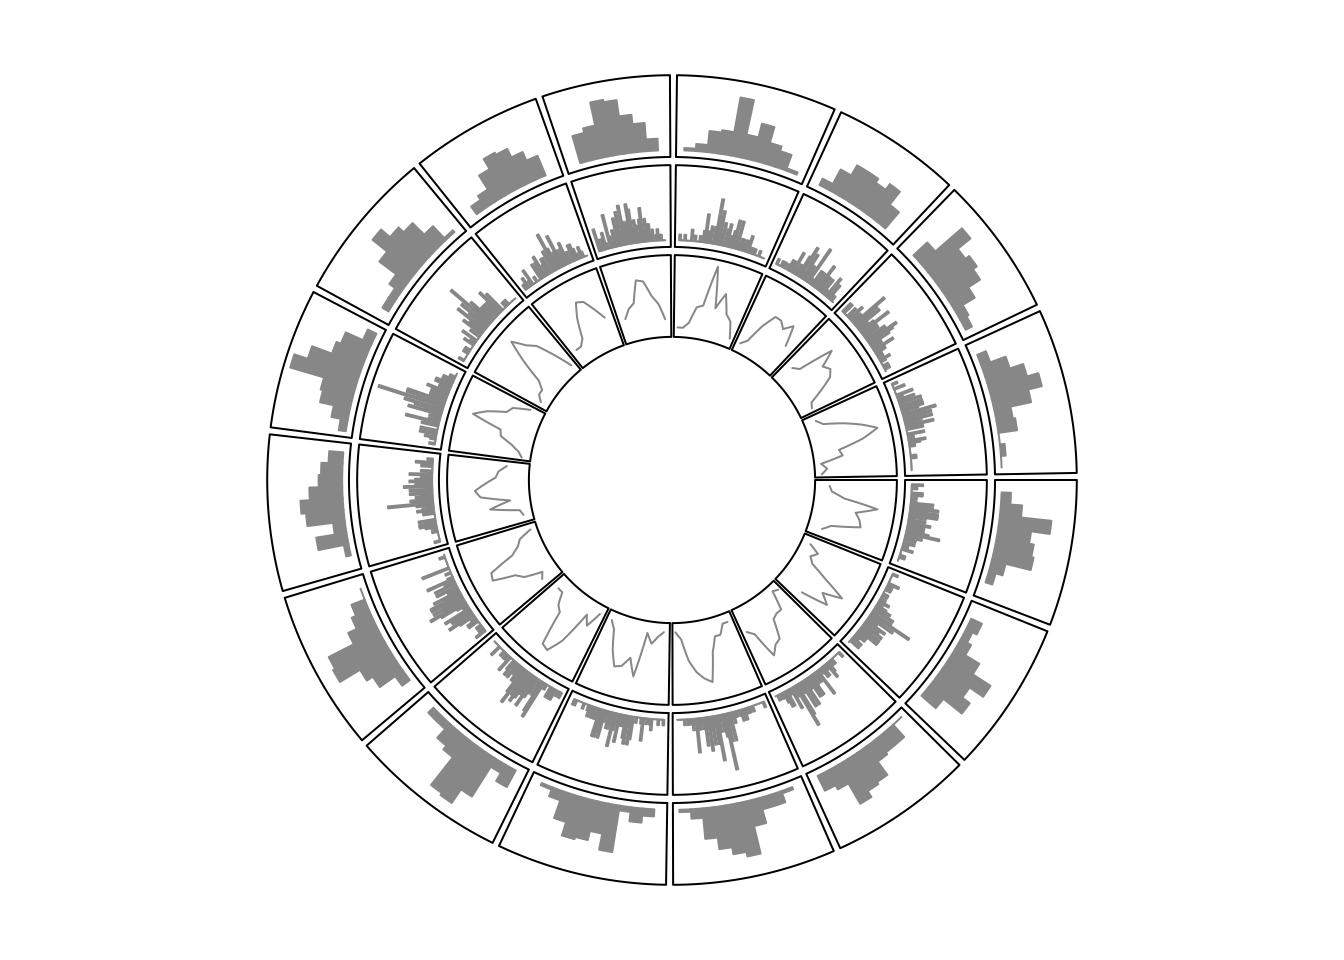
\includegraphics{05-implement-high-level-plots_files/figure-latex/circular-histograms-1} 

}

\caption{Histograms on circular layout.}\label{fig:circular-histograms}
\end{figure}

\begin{Shaded}
\begin{Highlighting}[]
\KeywordTok{circos.clear}\NormalTok{()}
\end{Highlighting}
\end{Shaded}

\section{Phylogenetic trees}\label{phylogenetic-trees}

Circular dendrograms have many applications, one of which is to
visualize phylogenetic trees. Basically, a phylogenetic tree is a
dendrogram which is a combination of lines. In R, there are several
classes that describe such type of tree such as \texttt{hclust},
\texttt{dendrogram} and \texttt{phylo}. In this example, we will
demonstrate how to draw the tree from the \texttt{dendrogram} class.
Nevertheless, other classes can be converted to \texttt{dendrogram}
without too much difficulty.

The \texttt{bird.orders} data we are using here is from \textbf{ape}
package. This data set is related to species of birds.

\begin{Shaded}
\begin{Highlighting}[]
\KeywordTok{library}\NormalTok{(ape)}
\KeywordTok{data}\NormalTok{(bird.orders)}
\NormalTok{hc =}\StringTok{ }\KeywordTok{as.hclust}\NormalTok{(bird.orders)}
\end{Highlighting}
\end{Shaded}

We split the tree into six sub trees by \texttt{cutree()} and convert
the data into a \texttt{dendrogram} object.

\begin{Shaded}
\begin{Highlighting}[]
\NormalTok{labels =}\StringTok{ }\NormalTok{hc}\OperatorTok{$}\NormalTok{labels  }\CommentTok{# name of birds}
\NormalTok{ct =}\StringTok{ }\KeywordTok{cutree}\NormalTok{(hc, }\DecValTok{6}\NormalTok{)  }\CommentTok{# cut tree into 6 pieces}
\NormalTok{n =}\StringTok{ }\KeywordTok{length}\NormalTok{(labels)  }\CommentTok{# number of bird species}
\NormalTok{dend =}\StringTok{ }\KeywordTok{as.dendrogram}\NormalTok{(hc)}
\end{Highlighting}
\end{Shaded}

As we mentioned before, the x-value for the phylogenetic tree is in fact
index. Thus, the x-lim is just the minimum and maximum index of labels
in the tree. Since there is only one phylogenetic tree, we only need one
``big'' sector.

In the first track, we plot the name of each bird, with different colors
to represent different sub trees.

\begin{Shaded}
\begin{Highlighting}[]
\KeywordTok{circos.par}\NormalTok{(}\DataTypeTok{cell.padding =} \KeywordTok{c}\NormalTok{(}\DecValTok{0}\NormalTok{, }\DecValTok{0}\NormalTok{, }\DecValTok{0}\NormalTok{, }\DecValTok{0}\NormalTok{))}
\KeywordTok{circos.initialize}\NormalTok{(}\DataTypeTok{factors =} \StringTok{"a"}\NormalTok{, }\DataTypeTok{xlim =} \KeywordTok{c}\NormalTok{(}\DecValTok{0}\NormalTok{, n)) }\CommentTok{# only one sector}
\KeywordTok{circos.track}\NormalTok{(}\DataTypeTok{ylim =} \KeywordTok{c}\NormalTok{(}\DecValTok{0}\NormalTok{, }\DecValTok{1}\NormalTok{), }\DataTypeTok{bg.border =} \OtherTok{NA}\NormalTok{, }\DataTypeTok{track.height =} \FloatTok{0.3}\NormalTok{, }
    \DataTypeTok{panel.fun =} \ControlFlowTok{function}\NormalTok{(x, y) \{}
        \ControlFlowTok{for}\NormalTok{(i }\ControlFlowTok{in} \KeywordTok{seq_len}\NormalTok{(n)) \{}
            \KeywordTok{circos.text}\NormalTok{(i}\OperatorTok{-}\FloatTok{0.5}\NormalTok{, }\DecValTok{0}\NormalTok{, labels[i], }\DataTypeTok{adj =} \KeywordTok{c}\NormalTok{(}\DecValTok{0}\NormalTok{, }\FloatTok{0.5}\NormalTok{), }
                \DataTypeTok{facing =} \StringTok{"clockwise"}\NormalTok{, }\DataTypeTok{niceFacing =} \OtherTok{TRUE}\NormalTok{,}
                \DataTypeTok{col =}\NormalTok{ ct[labels[i]], }\DataTypeTok{cex =} \FloatTok{0.5}\NormalTok{)}
\NormalTok{        \}}
\NormalTok{\})}
\end{Highlighting}
\end{Shaded}

In the above code, setting \texttt{xlim} to \texttt{c(0,\ n)} is very
important because the leaves of the dendrogram are drawn at
\texttt{x\ =\ seq(0.5,\ n\ -\ 0.5)}.

In the second track, we plot the circular dendrogram by
\texttt{circos.dendrogram()} (Figure \ref{fig:phylogenetic-tree} left).
You can render the dendrogram by \textbf{dendextend} package.

\begin{Shaded}
\begin{Highlighting}[]
\KeywordTok{suppressPackageStartupMessages}\NormalTok{(}\KeywordTok{library}\NormalTok{(dendextend))}
\NormalTok{dend =}\StringTok{ }\KeywordTok{color_branches}\NormalTok{(dend, }\DataTypeTok{k =} \DecValTok{6}\NormalTok{, }\DataTypeTok{col =} \DecValTok{1}\OperatorTok{:}\DecValTok{6}\NormalTok{)}
\NormalTok{dend_height =}\StringTok{ }\KeywordTok{attr}\NormalTok{(dend, }\StringTok{"height"}\NormalTok{)}
\KeywordTok{circos.track}\NormalTok{(}\DataTypeTok{ylim =} \KeywordTok{c}\NormalTok{(}\DecValTok{0}\NormalTok{, dend_height), }\DataTypeTok{bg.border =} \OtherTok{NA}\NormalTok{, }
    \DataTypeTok{track.height =} \FloatTok{0.4}\NormalTok{, }\DataTypeTok{panel.fun =} \ControlFlowTok{function}\NormalTok{(x, y) \{}
        \KeywordTok{circos.dendrogram}\NormalTok{(dend)}
\NormalTok{\})}
\KeywordTok{circos.clear}\NormalTok{()}
\end{Highlighting}
\end{Shaded}

By default, dendrograms are facing outside of the circle (so that the
labels should also be added outside the dendrogram). In
\texttt{circos.dendrogram()}, you can set \texttt{facing} argument to
\texttt{inside} to make them facing inside. In this case, dendrogram
track is added first and labels are added later (Figure
\ref{fig:phylogenetic-tree} right).

\begin{Shaded}
\begin{Highlighting}[]
\KeywordTok{circos.dendrogram}\NormalTok{(dend, }\DataTypeTok{facing =} \StringTok{"inside"}\NormalTok{)}
\end{Highlighting}
\end{Shaded}

\begin{figure}

{\centering 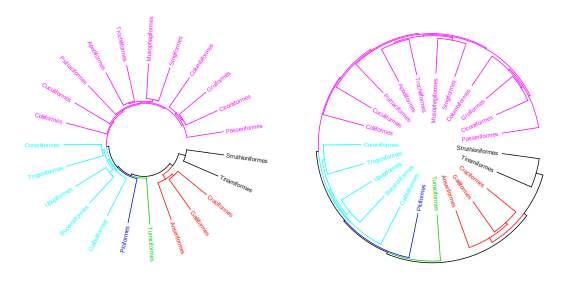
\includegraphics{05-implement-high-level-plots_files/figure-latex/phylogenetic-tree-1} 

}

\caption{A circular phylogenetic tree.}\label{fig:phylogenetic-tree}
\end{figure}

If you look at the souce code of \texttt{circos.dendrogram()} and
replace \texttt{circos.lines()} to \texttt{lines()}, actually the
function can correctly make a dendrogram in the normal coordinate.

With the flexibility of \textbf{circlize} package, it is easy to add
more tracks if you want to add more corresponded information for the
dendrogram to the plot.

\section{Heatmaps}\label{heatmaps}

Heatmaps, and sometimes combined with dendrograms are frequently used to
visualize e.g.~gene expression. Heatmaps are basically composed by
rectangles, thus, they can be implemented by \texttt{circos.rect()}.

In following example, we make a circular plot with two heatmaps. First
we generate the two matrix and perform clustring on the two matrix.

\begin{Shaded}
\begin{Highlighting}[]
\NormalTok{mat =}\StringTok{ }\KeywordTok{matrix}\NormalTok{(}\KeywordTok{rnorm}\NormalTok{(}\DecValTok{100}\OperatorTok{*}\DecValTok{10}\NormalTok{), }\DataTypeTok{nrow =} \DecValTok{10}\NormalTok{, }\DataTypeTok{ncol =} \DecValTok{100}\NormalTok{)}
\NormalTok{col_fun =}\StringTok{ }\KeywordTok{colorRamp2}\NormalTok{(}\KeywordTok{c}\NormalTok{(}\OperatorTok{-}\DecValTok{2}\NormalTok{, }\DecValTok{0}\NormalTok{, }\DecValTok{2}\NormalTok{), }\KeywordTok{c}\NormalTok{(}\StringTok{"green"}\NormalTok{, }\StringTok{"black"}\NormalTok{, }\StringTok{"red"}\NormalTok{))}
\NormalTok{factors =}\StringTok{ }\KeywordTok{rep}\NormalTok{(letters[}\DecValTok{1}\OperatorTok{:}\DecValTok{2}\NormalTok{], }\DataTypeTok{times =} \KeywordTok{c}\NormalTok{(}\DecValTok{30}\NormalTok{, }\DecValTok{70}\NormalTok{))}
\NormalTok{mat_list =}\StringTok{ }\KeywordTok{list}\NormalTok{(}\DataTypeTok{a =}\NormalTok{ mat[, factors }\OperatorTok{==}\StringTok{ "a"}\NormalTok{],}
                \DataTypeTok{b =}\NormalTok{ mat[, factors }\OperatorTok{==}\StringTok{ "b"}\NormalTok{])}
\NormalTok{dend_list =}\StringTok{ }\KeywordTok{list}\NormalTok{(}\DataTypeTok{a =} \KeywordTok{as.dendrogram}\NormalTok{(}\KeywordTok{hclust}\NormalTok{(}\KeywordTok{dist}\NormalTok{(}\KeywordTok{t}\NormalTok{(mat_list[[}\StringTok{"a"}\NormalTok{]])))),}
                 \DataTypeTok{b =} \KeywordTok{as.dendrogram}\NormalTok{(}\KeywordTok{hclust}\NormalTok{(}\KeywordTok{dist}\NormalTok{(}\KeywordTok{t}\NormalTok{(mat_list[[}\StringTok{"b"}\NormalTok{]])))))}
\end{Highlighting}
\end{Shaded}

In the first track, columns in the matrix are adjusted by the
clustering. Also note we use \texttt{circos.rect()} in a vectorized way.

\begin{Shaded}
\begin{Highlighting}[]
\KeywordTok{circos.par}\NormalTok{(}\DataTypeTok{cell.padding =} \KeywordTok{c}\NormalTok{(}\DecValTok{0}\NormalTok{, }\DecValTok{0}\NormalTok{, }\DecValTok{0}\NormalTok{, }\DecValTok{0}\NormalTok{), }\DataTypeTok{gap.degree =} \DecValTok{5}\NormalTok{)}
\KeywordTok{circos.initialize}\NormalTok{(factors, }\DataTypeTok{xlim =} \KeywordTok{cbind}\NormalTok{(}\KeywordTok{c}\NormalTok{(}\DecValTok{0}\NormalTok{, }\DecValTok{0}\NormalTok{), }\KeywordTok{table}\NormalTok{(factors)))}
\KeywordTok{circos.track}\NormalTok{(}\DataTypeTok{ylim =} \KeywordTok{c}\NormalTok{(}\DecValTok{0}\NormalTok{, }\DecValTok{10}\NormalTok{), }\DataTypeTok{bg.border =} \OtherTok{NA}\NormalTok{, }\DataTypeTok{panel.fun =} \ControlFlowTok{function}\NormalTok{(x, y) \{}
\NormalTok{    sector.index =}\StringTok{ }\NormalTok{CELL_META}\OperatorTok{$}\NormalTok{sector.index}
\NormalTok{    m =}\StringTok{ }\NormalTok{mat_list[[sector.index]]}
\NormalTok{    dend =}\StringTok{ }\NormalTok{dend_list[[sector.index]]}

\NormalTok{    m2 =}\StringTok{ }\NormalTok{m[, }\KeywordTok{order.dendrogram}\NormalTok{(dend)]}
\NormalTok{    col_mat =}\StringTok{ }\KeywordTok{col_fun}\NormalTok{(m2)}
\NormalTok{    nr =}\StringTok{ }\KeywordTok{nrow}\NormalTok{(m2)}
\NormalTok{    nc =}\StringTok{ }\KeywordTok{ncol}\NormalTok{(m2)}
    \ControlFlowTok{for}\NormalTok{(i }\ControlFlowTok{in} \DecValTok{1}\OperatorTok{:}\NormalTok{nr) \{}
        \KeywordTok{circos.rect}\NormalTok{(}\DecValTok{1}\OperatorTok{:}\NormalTok{nc }\OperatorTok{-}\StringTok{ }\DecValTok{1}\NormalTok{, }\KeywordTok{rep}\NormalTok{(nr }\OperatorTok{-}\StringTok{ }\NormalTok{i, nc), }
            \DecValTok{1}\OperatorTok{:}\NormalTok{nc, }\KeywordTok{rep}\NormalTok{(nr }\OperatorTok{-}\StringTok{ }\NormalTok{i }\OperatorTok{+}\StringTok{ }\DecValTok{1}\NormalTok{, nc), }
            \DataTypeTok{border =}\NormalTok{ col_mat[i, ], }\DataTypeTok{col =}\NormalTok{ col_mat[i, ])}
\NormalTok{    \}}
\NormalTok{\})}
\end{Highlighting}
\end{Shaded}

Since there are two dendrograms, it is important to make the height of
both dendrogram in a same scale. We calculate the maximum height of the
two dendrograms and set it to \texttt{ylim} of the second track (Figure
\ref{fig:circular-heatmap}).

\begin{Shaded}
\begin{Highlighting}[]
\NormalTok{max_height =}\StringTok{ }\KeywordTok{max}\NormalTok{(}\KeywordTok{sapply}\NormalTok{(dend_list, }\ControlFlowTok{function}\NormalTok{(x) }\KeywordTok{attr}\NormalTok{(x, }\StringTok{"height"}\NormalTok{)))}
\KeywordTok{circos.track}\NormalTok{(}\DataTypeTok{ylim =} \KeywordTok{c}\NormalTok{(}\DecValTok{0}\NormalTok{, max_height), }\DataTypeTok{bg.border =} \OtherTok{NA}\NormalTok{, }\DataTypeTok{track.height =} \FloatTok{0.3}\NormalTok{, }
    \DataTypeTok{panel.fun =} \ControlFlowTok{function}\NormalTok{(x, y) \{}

\NormalTok{        sector.index =}\StringTok{ }\KeywordTok{get.cell.meta.data}\NormalTok{(}\StringTok{"sector.index"}\NormalTok{)}
\NormalTok{        dend =}\StringTok{ }\NormalTok{dend_list[[sector.index]]}
        \KeywordTok{circos.dendrogram}\NormalTok{(dend, }\DataTypeTok{max_height =}\NormalTok{ max_height)}
\NormalTok{\})}
\KeywordTok{circos.clear}\NormalTok{()}
\end{Highlighting}
\end{Shaded}

\begin{figure}

{\centering 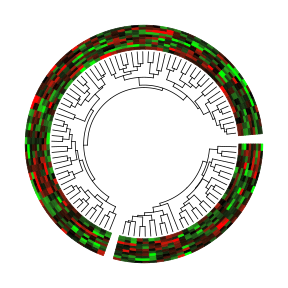
\includegraphics{05-implement-high-level-plots_files/figure-latex/circular-heatmap-1} 

}

\caption{Circular heatmaps.}\label{fig:circular-heatmap}
\end{figure}

\chapter{Advanced layout}\label{advanced-layout}

\section{Zooming of sectors}\label{zooming-of-sectors}

In this section, we will introduce how to zoom sectors and put the
zoomed sectors at the same track as the original sectors.

Under the default settings, width of sectors are calculated according to
the data range in corresponding categories. Normally it is not a good
idea to manually modify the default sector width since it reflects
useful information of your data. However, sometimes manually modifying
the width of sectors can make more advanced plots, e.g.~zoomings.

The basic idea for zooming is to put original sectors on part of the
circle and put the zoomed sectors on the other part, so that in the
original sectors, widths are still proportional to their data ranges,
and in the zoomed sectors, the widths are also proportional to the data
ranges in the zoomed sectors.

This type of zooming is rather simple to implement. All we need to do is
to copy the data which corresponds to the zoomed sectors, assign new
category names to them and append to the original data. The good thing
is since the data in the zoomed sectors is exactly the same as the
original sectors, if you treat them as normal categories, the graphics
will be exactly the same as in the original sectors, but with x
direction zoomed.

Following example shows more clearly the basic idea of this
``horizontal'' zooming.

We first generate a data frame with six categories.

\begin{Shaded}
\begin{Highlighting}[]
\KeywordTok{set.seed}\NormalTok{(}\DecValTok{123}\NormalTok{)}
\NormalTok{df =}\StringTok{ }\KeywordTok{data.frame}\NormalTok{(}
    \DataTypeTok{factors =} \KeywordTok{sample}\NormalTok{(letters[}\DecValTok{1}\OperatorTok{:}\DecValTok{6}\NormalTok{], }\DecValTok{400}\NormalTok{, }\DataTypeTok{replace =} \OtherTok{TRUE}\NormalTok{),}
    \DataTypeTok{x =} \KeywordTok{rnorm}\NormalTok{(}\DecValTok{400}\NormalTok{),}
    \DataTypeTok{y =} \KeywordTok{rnorm}\NormalTok{(}\DecValTok{400}\NormalTok{),}
    \DataTypeTok{stringsAsFactors =} \OtherTok{FALSE}
\NormalTok{)}
\end{Highlighting}
\end{Shaded}

We want to zoom sector a and the first 10 points in sector b. First we
extract these data and format as a new data frame.

\begin{Shaded}
\begin{Highlighting}[]
\NormalTok{zoom_df_a =}\StringTok{ }\NormalTok{df[df}\OperatorTok{$}\NormalTok{factors }\OperatorTok{==}\StringTok{ "a"}\NormalTok{, ]}
\NormalTok{zoom_df_b =}\StringTok{ }\NormalTok{df[df}\OperatorTok{$}\NormalTok{factors }\OperatorTok{==}\StringTok{ "b"}\NormalTok{, ]}
\NormalTok{zoom_df_b =}\StringTok{ }\NormalTok{zoom_df_b[}\KeywordTok{order}\NormalTok{(zoom_df_b[, }\DecValTok{2}\NormalTok{])[}\DecValTok{1}\OperatorTok{:}\DecValTok{10}\NormalTok{], ]}
\NormalTok{zoom_df =}\StringTok{ }\KeywordTok{rbind}\NormalTok{(zoom_df_a, zoom_df_b)}
\end{Highlighting}
\end{Shaded}

Then we need to change the sector names in the zoomed data frame. Here
we just simply add ``zoom\_'' prefix to the original names to show that
they are ``zoomed'' sectors. After that, it is attached to the original
data frame.

\begin{Shaded}
\begin{Highlighting}[]
\NormalTok{zoom_df}\OperatorTok{$}\NormalTok{factors =}\StringTok{ }\KeywordTok{paste0}\NormalTok{(}\StringTok{"zoom_"}\NormalTok{, zoom_df}\OperatorTok{$}\NormalTok{factors)}
\NormalTok{df2 =}\StringTok{ }\KeywordTok{rbind}\NormalTok{(df, zoom_df)}
\end{Highlighting}
\end{Shaded}

In this example, we will put the original cells in the left half of the
circle and the zoomed sectors in the right. As we have already mentioned
before, we simply normalize the width of normal sectors and normalize
the width of zoomed sectors separately. Note now the sum of the sector
width for the original sectors is 1 and the sum of sector width for the
zoomed sectors is 1, which means these two types of sectors have their
own half circle.

You may notice the sum of the \texttt{sector.width} is not idential to
1. This is fine, they will be further normalized to 1 internally.

Strictly speaking, since the gaps between sectors are not taken into
consideration, the width of the original sectors are not exactly 180
degree, but the real value is quite close to it.

\begin{Shaded}
\begin{Highlighting}[]
\NormalTok{xrange =}\StringTok{ }\KeywordTok{tapply}\NormalTok{(df2}\OperatorTok{$}\NormalTok{x, df2}\OperatorTok{$}\NormalTok{factors, }\ControlFlowTok{function}\NormalTok{(x) }\KeywordTok{max}\NormalTok{(x) }\OperatorTok{-}\StringTok{ }\KeywordTok{min}\NormalTok{(x))}
\NormalTok{normal_sector_index =}\StringTok{ }\KeywordTok{unique}\NormalTok{(df}\OperatorTok{$}\NormalTok{factors)}
\NormalTok{zoomed_sector_index =}\StringTok{ }\KeywordTok{unique}\NormalTok{(zoom_df}\OperatorTok{$}\NormalTok{factors)}
\NormalTok{sector.width =}\StringTok{ }\KeywordTok{c}\NormalTok{(xrange[normal_sector_index] }\OperatorTok{/}\StringTok{ }\KeywordTok{sum}\NormalTok{(xrange[normal_sector_index]), }
\NormalTok{                 xrange[zoomed_sector_index] }\OperatorTok{/}\StringTok{ }\KeywordTok{sum}\NormalTok{(xrange[zoomed_sector_index]))}
\NormalTok{sector.width}
\end{Highlighting}
\end{Shaded}

\begin{verbatim}
##         b         e         c         f         a         d    zoom_a 
## 0.1685162 0.1765301 0.1732999 0.1705148 0.1518915 0.1592475 0.8097123 
##    zoom_b 
## 0.1902877
\end{verbatim}

What to do next is just to make the circular plot in the normal way. All
the graphics in sector a and b will be automatically zoomed to sector
``zoom\_a'' and ``zoom\_b''.

In following code, since the sector names are added outside the first
track, \texttt{points.overflow.warning} is set to \texttt{FALSE} to turn
off the warning messages.

\begin{Shaded}
\begin{Highlighting}[]
\KeywordTok{circos.par}\NormalTok{(}\DataTypeTok{start.degree =} \DecValTok{90}\NormalTok{, }\DataTypeTok{points.overflow.warning =} \OtherTok{FALSE}\NormalTok{)}
\KeywordTok{circos.initialize}\NormalTok{(df2}\OperatorTok{$}\NormalTok{factors, }\DataTypeTok{x =}\NormalTok{ df2}\OperatorTok{$}\NormalTok{x, }\DataTypeTok{sector.width =}\NormalTok{ sector.width)}
\KeywordTok{circos.track}\NormalTok{(df2}\OperatorTok{$}\NormalTok{factors, }\DataTypeTok{x =}\NormalTok{ df2}\OperatorTok{$}\NormalTok{x, }\DataTypeTok{y =}\NormalTok{ df2}\OperatorTok{$}\NormalTok{y, }
    \DataTypeTok{panel.fun =} \ControlFlowTok{function}\NormalTok{(x, y) \{}
    \KeywordTok{circos.points}\NormalTok{(x, y, }\DataTypeTok{col =} \StringTok{"red"}\NormalTok{, }\DataTypeTok{pch =} \DecValTok{16}\NormalTok{, }\DataTypeTok{cex =} \FloatTok{0.5}\NormalTok{)}
    \KeywordTok{circos.text}\NormalTok{(CELL_META}\OperatorTok{$}\NormalTok{xcenter, CELL_META}\OperatorTok{$}\NormalTok{cell.ylim[}\DecValTok{2}\NormalTok{] }\OperatorTok{+}\StringTok{ }\KeywordTok{uy}\NormalTok{(}\DecValTok{2}\NormalTok{, }\StringTok{"mm"}\NormalTok{), }
\NormalTok{        CELL_META}\OperatorTok{$}\NormalTok{sector.index, }\DataTypeTok{niceFacing =} \OtherTok{TRUE}\NormalTok{)}
\NormalTok{\})}
\end{Highlighting}
\end{Shaded}

Adding links from original sectors to zoomed sectors is a good idea to
show where the zooming occurs (Figure \ref{fig:circlize-zoom}). Notice
that we manually adjust the position of one end of the sector b link.

\begin{Shaded}
\begin{Highlighting}[]
\KeywordTok{circos.link}\NormalTok{(}\StringTok{"a"}\NormalTok{, }\KeywordTok{get.cell.meta.data}\NormalTok{(}\StringTok{"cell.xlim"}\NormalTok{, }\DataTypeTok{sector.index =} \StringTok{"a"}\NormalTok{),}
    \StringTok{"zoom_a"}\NormalTok{, }\KeywordTok{get.cell.meta.data}\NormalTok{(}\StringTok{"cell.xlim"}\NormalTok{, }\DataTypeTok{sector.index =} \StringTok{"zoom_a"}\NormalTok{),}
    \DataTypeTok{border =} \OtherTok{NA}\NormalTok{, }\DataTypeTok{col =} \StringTok{"#00000020"}\NormalTok{)}
\KeywordTok{circos.link}\NormalTok{(}\StringTok{"b"}\NormalTok{, }\KeywordTok{c}\NormalTok{(zoom_df_b[}\DecValTok{1}\NormalTok{, }\DecValTok{2}\NormalTok{], zoom_df_b[}\DecValTok{10}\NormalTok{, }\DecValTok{2}\NormalTok{]),}
    \StringTok{"zoom_b"}\NormalTok{, }\KeywordTok{get.cell.meta.data}\NormalTok{(}\StringTok{"cell.xlim"}\NormalTok{, }\DataTypeTok{sector.index =} \StringTok{"zoom_b"}\NormalTok{),}
    \DataTypeTok{rou1 =} \KeywordTok{get.cell.meta.data}\NormalTok{(}\StringTok{"cell.top.radius"}\NormalTok{, }\DataTypeTok{sector.index =} \StringTok{"b"}\NormalTok{),}
    \DataTypeTok{border =} \OtherTok{NA}\NormalTok{, }\DataTypeTok{col =} \StringTok{"#00000020"}\NormalTok{)}
\KeywordTok{circos.clear}\NormalTok{()}
\end{Highlighting}
\end{Shaded}

\begin{figure}

{\centering 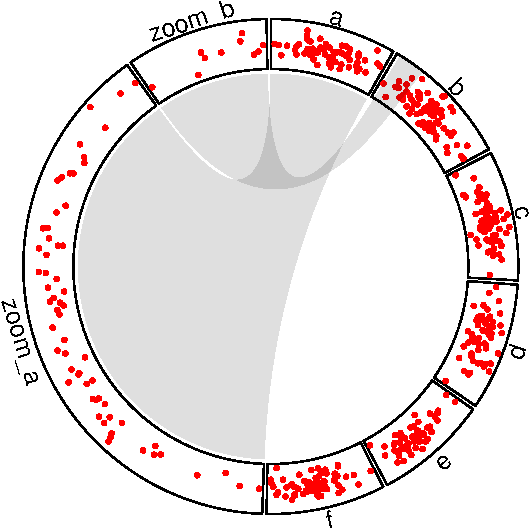
\includegraphics{06-advanced-usage_files/figure-latex/circlize-zoom-1} 

}

\caption{Zoom sectors.}\label{fig:circlize-zoom}
\end{figure}

Chapter \ref{nested-zooming} introduces another type of zooming by
combining two circular plots.

\section{Visualize part of the circle}\label{part-circle}

\texttt{canvas.xlim} and \texttt{canvas.ylim} parameters in
\texttt{circos.par()} are useful to generate plots only in part of the
circle. As mentioned in previews chapters, the circular plot is always
drawn in a canvas where x values range from -1 to 1 and y values range
from -1 to 1. Thus, if \texttt{canvas.xlim} and \texttt{canvas.ylim} are
all set to \texttt{c(0,\ 1)}, which means, the canvas is restricted to
the right top part, then only sectors between 0 to 90 degree are visible
(Figure \ref{fig:circlize-part}).

\begin{figure}

{\centering 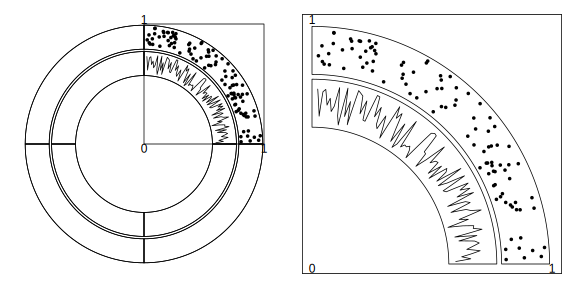
\includegraphics{06-advanced-usage_files/figure-latex/circlize-part-1} 

}

\caption{One quarter of the circle.}\label{fig:circlize-part}
\end{figure}

To make the right plot in Figure \ref{fig:circlize-part}, we only need
to set one sector in the layout and set \texttt{gap.after} to 270. (One
sector with \texttt{gap.after} of 270 degree means the width of this
sector is exactly 90 degree.)

\begin{Shaded}
\begin{Highlighting}[]
\KeywordTok{circos.par}\NormalTok{(}\StringTok{"canvas.xlim"}\NormalTok{ =}\StringTok{ }\KeywordTok{c}\NormalTok{(}\DecValTok{0}\NormalTok{, }\DecValTok{1}\NormalTok{), }\StringTok{"canvas.ylim"}\NormalTok{ =}\StringTok{ }\KeywordTok{c}\NormalTok{(}\DecValTok{0}\NormalTok{, }\DecValTok{1}\NormalTok{),}
    \StringTok{"start.degree"}\NormalTok{ =}\StringTok{ }\DecValTok{90}\NormalTok{, }\StringTok{"gap.after"}\NormalTok{ =}\StringTok{ }\DecValTok{270}\NormalTok{)}
\NormalTok{factors =}\StringTok{ "a"} \CommentTok{# this is the name of your sector}
\KeywordTok{circos.initialize}\NormalTok{(}\DataTypeTok{factors =}\NormalTok{ factors, }\DataTypeTok{xlim =}\NormalTok{ ...)}
\NormalTok{...}
\end{Highlighting}
\end{Shaded}

Similar idea can be applied to the circle where in some tracks, only a
subset of cells are needed. Gererally there are two ways. The first way
is to create the track and add graphics with subset of data that only
corresponds to the cells that are needed. And the second way is to
create an empty track first and customize the cells by
\texttt{circos.update()}. Following code illustrates the two methods
(Figure \ref{fig:circlize-part2}).

\begin{Shaded}
\begin{Highlighting}[]
\NormalTok{factors =}\StringTok{ }\NormalTok{letters[}\DecValTok{1}\OperatorTok{:}\DecValTok{4}\NormalTok{]}
\KeywordTok{circos.initialize}\NormalTok{(}\DataTypeTok{factors =}\NormalTok{ factors, }\DataTypeTok{xlim =} \KeywordTok{c}\NormalTok{(}\DecValTok{0}\NormalTok{, }\DecValTok{1}\NormalTok{))}

\CommentTok{# directly specify the subset of data}
\NormalTok{df =}\StringTok{ }\KeywordTok{data.frame}\NormalTok{(}\DataTypeTok{factors =} \KeywordTok{rep}\NormalTok{(}\StringTok{"a"}\NormalTok{, }\DecValTok{100}\NormalTok{),}
                \DataTypeTok{x =} \KeywordTok{runif}\NormalTok{(}\DecValTok{100}\NormalTok{),}
                \DataTypeTok{y =} \KeywordTok{runif}\NormalTok{(}\DecValTok{100}\NormalTok{))}
\KeywordTok{circos.track}\NormalTok{(df}\OperatorTok{$}\NormalTok{factors, }\DataTypeTok{x =}\NormalTok{ df}\OperatorTok{$}\NormalTok{x, }\DataTypeTok{y =}\NormalTok{ df}\OperatorTok{$}\NormalTok{y, }
    \DataTypeTok{panel.fun =} \ControlFlowTok{function}\NormalTok{(x, y) \{}
        \KeywordTok{circos.points}\NormalTok{(x, y, }\DataTypeTok{pch =} \DecValTok{16}\NormalTok{, }\DataTypeTok{cex =} \FloatTok{0.5}\NormalTok{)}
\NormalTok{\})}

\CommentTok{# create empty track first then fill graphics in the cell}
\KeywordTok{circos.track}\NormalTok{(}\DataTypeTok{ylim =} \KeywordTok{range}\NormalTok{(df}\OperatorTok{$}\NormalTok{y), }\DataTypeTok{bg.border =} \OtherTok{NA}\NormalTok{)}
\KeywordTok{circos.update}\NormalTok{(}\DataTypeTok{sector.index =} \StringTok{"a"}\NormalTok{, }\DataTypeTok{bg.border =} \StringTok{"black"}\NormalTok{)}
\KeywordTok{circos.points}\NormalTok{(df}\OperatorTok{$}\NormalTok{x, df}\OperatorTok{$}\NormalTok{y, }\DataTypeTok{pch =} \DecValTok{16}\NormalTok{, }\DataTypeTok{cex =} \FloatTok{0.5}\NormalTok{)}

\KeywordTok{circos.track}\NormalTok{(}\DataTypeTok{factors =}\NormalTok{ factors, }\DataTypeTok{ylim =} \KeywordTok{c}\NormalTok{(}\DecValTok{0}\NormalTok{, }\DecValTok{1}\NormalTok{))}
\KeywordTok{circos.track}\NormalTok{(}\DataTypeTok{factors =}\NormalTok{ factors, }\DataTypeTok{ylim =} \KeywordTok{c}\NormalTok{(}\DecValTok{0}\NormalTok{, }\DecValTok{1}\NormalTok{))}
\end{Highlighting}
\end{Shaded}

\begin{figure}

{\centering 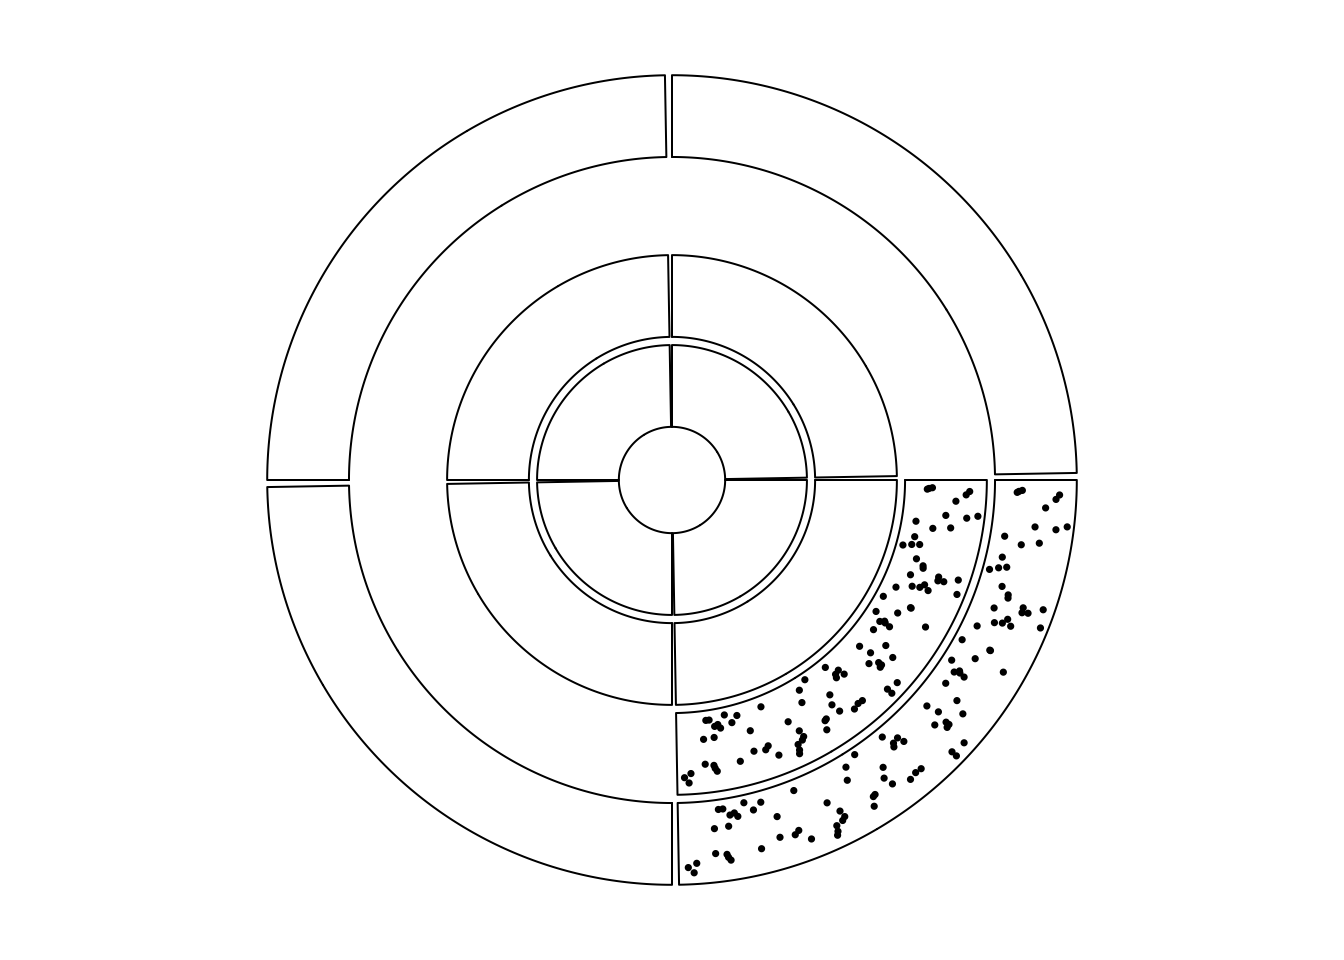
\includegraphics{06-advanced-usage_files/figure-latex/circlize-part2-1} 

}

\caption{Show subset of cells in tracks.}\label{fig:circlize-part2}
\end{figure}

\begin{Shaded}
\begin{Highlighting}[]
\KeywordTok{circos.clear}\NormalTok{()}
\end{Highlighting}
\end{Shaded}

\section{Combine multiple circular plots}\label{combine-circular-plots}

\textbf{circlize} finally makes the circular plot in the base R graphic
system. Seperated circular plots actually can be put in a same page by
some tricks from the base graphic system. Here the key is
\texttt{par(new\ =\ TRUE)} which allows to draw a new figure as a new
layer directly on the previous canvas region. By setting different
\texttt{canvas.xlim} and \texttt{canvas.ylim}, it allows to make more
complex plots which include more than one circular plots.

Folowing code shows how the two independent circualr plots are added and
nested. Figure \ref{fig:circlize-nested} illustrates the invisible
canvas coordinate and how the two circular plots overlap.

\begin{Shaded}
\begin{Highlighting}[]
\NormalTok{factors =}\StringTok{ }\NormalTok{letters[}\DecValTok{1}\OperatorTok{:}\DecValTok{4}\NormalTok{]}
\KeywordTok{circos.initialize}\NormalTok{(}\DataTypeTok{factors =}\NormalTok{ factors, }\DataTypeTok{xlim =} \KeywordTok{c}\NormalTok{(}\DecValTok{0}\NormalTok{, }\DecValTok{1}\NormalTok{))}
\KeywordTok{circos.track}\NormalTok{(}\DataTypeTok{ylim =} \KeywordTok{c}\NormalTok{(}\DecValTok{0}\NormalTok{, }\DecValTok{1}\NormalTok{), }\DataTypeTok{panel.fun =} \ControlFlowTok{function}\NormalTok{(x, y) \{}
    \KeywordTok{circos.text}\NormalTok{(}\FloatTok{0.5}\NormalTok{, }\FloatTok{0.5}\NormalTok{, }\StringTok{"outer circos"}\NormalTok{, }\DataTypeTok{niceFacing =} \OtherTok{TRUE}\NormalTok{)}
\NormalTok{\})}
\KeywordTok{circos.clear}\NormalTok{()}

\KeywordTok{par}\NormalTok{(}\DataTypeTok{new =} \OtherTok{TRUE}\NormalTok{) }\CommentTok{# <- magic}
\KeywordTok{circos.par}\NormalTok{(}\StringTok{"canvas.xlim"}\NormalTok{ =}\StringTok{ }\KeywordTok{c}\NormalTok{(}\OperatorTok{-}\DecValTok{2}\NormalTok{, }\DecValTok{2}\NormalTok{), }\StringTok{"canvas.ylim"}\NormalTok{ =}\StringTok{ }\KeywordTok{c}\NormalTok{(}\OperatorTok{-}\DecValTok{2}\NormalTok{, }\DecValTok{2}\NormalTok{))}
\NormalTok{factors =}\StringTok{ }\NormalTok{letters[}\DecValTok{1}\OperatorTok{:}\DecValTok{3}\NormalTok{]}
\KeywordTok{circos.initialize}\NormalTok{(}\DataTypeTok{factors =}\NormalTok{ factors, }\DataTypeTok{xlim =} \KeywordTok{c}\NormalTok{(}\DecValTok{0}\NormalTok{, }\DecValTok{1}\NormalTok{))}
\KeywordTok{circos.track}\NormalTok{(}\DataTypeTok{ylim =} \KeywordTok{c}\NormalTok{(}\DecValTok{0}\NormalTok{, }\DecValTok{1}\NormalTok{), }\DataTypeTok{panel.fun =} \ControlFlowTok{function}\NormalTok{(x, y) \{}
    \KeywordTok{circos.text}\NormalTok{(}\FloatTok{0.5}\NormalTok{, }\FloatTok{0.5}\NormalTok{, }\StringTok{"inner circos"}\NormalTok{, }\DataTypeTok{niceFacing =} \OtherTok{TRUE}\NormalTok{)}
\NormalTok{\})}
\KeywordTok{circos.clear}\NormalTok{()}
\end{Highlighting}
\end{Shaded}

\begin{figure}

{\centering 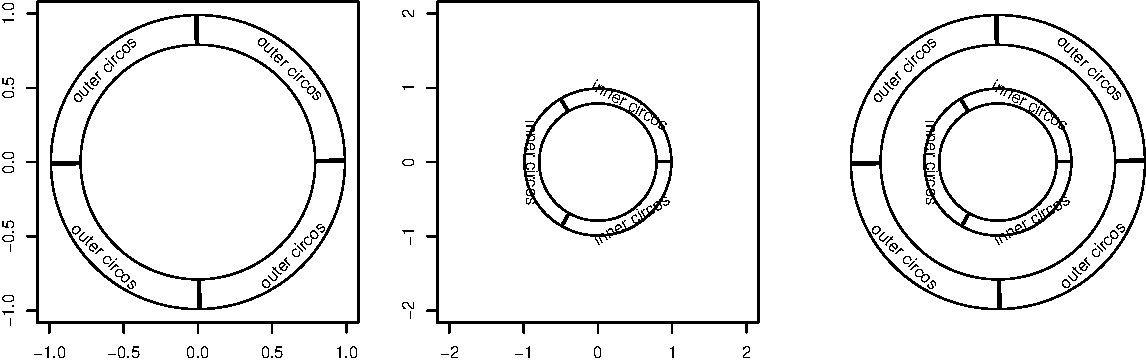
\includegraphics{06-advanced-usage_files/figure-latex/circlize-nested-1} 

}

\caption{Nested circular plots.}\label{fig:circlize-nested}
\end{figure}

The second example (Figure \ref{fig:circlize-separated}) makes a plot
where two circular plots separate from each other. You can use technique
introduced in Section \ref{part-circle} to only show part of the circle,
select proper \texttt{canvas.xlim} and \texttt{canvas.ylim}, and finally
arrange the two plots into one page. The source code for generating
Figure \ref{fig:circlize-separated} is at
\url{https://github.com/jokergoo/circlize_book/blob/master/src/intro-20-separated.R}.

\begin{figure}

{\centering 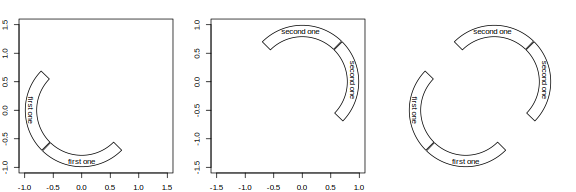
\includegraphics{06-advanced-usage_files/figure-latex/circlize-separated-1} 

}

\caption{Two separated circular plots}\label{fig:circlize-separated}
\end{figure}

The third example is to draw cells with different radius (Figure
\ref{fig:circlize-diff-radius}). In fact, it makes four circular plots
where only one sector for each plot is plotted.

\begin{Shaded}
\begin{Highlighting}[]
\NormalTok{factors =}\StringTok{ }\NormalTok{letters[}\DecValTok{1}\OperatorTok{:}\DecValTok{4}\NormalTok{]}
\NormalTok{lim =}\StringTok{ }\KeywordTok{c}\NormalTok{(}\DecValTok{1}\NormalTok{, }\FloatTok{1.1}\NormalTok{, }\FloatTok{1.2}\NormalTok{, }\FloatTok{1.3}\NormalTok{)}
\ControlFlowTok{for}\NormalTok{(i }\ControlFlowTok{in} \DecValTok{1}\OperatorTok{:}\DecValTok{4}\NormalTok{) \{}
    \KeywordTok{circos.par}\NormalTok{(}\StringTok{"canvas.xlim"}\NormalTok{ =}\StringTok{ }\KeywordTok{c}\NormalTok{(}\OperatorTok{-}\NormalTok{lim[i], lim[i]), }
        \StringTok{"canvas.ylim"}\NormalTok{ =}\StringTok{ }\KeywordTok{c}\NormalTok{(}\OperatorTok{-}\NormalTok{lim[i], lim[i]), }
        \StringTok{"track.height"}\NormalTok{ =}\StringTok{ }\FloatTok{0.4}\NormalTok{)}
    \KeywordTok{circos.initialize}\NormalTok{(}\DataTypeTok{factors =}\NormalTok{ factors, }\DataTypeTok{xlim =} \KeywordTok{c}\NormalTok{(}\DecValTok{0}\NormalTok{, }\DecValTok{1}\NormalTok{))}
    \KeywordTok{circos.track}\NormalTok{(}\DataTypeTok{ylim =} \KeywordTok{c}\NormalTok{(}\DecValTok{0}\NormalTok{, }\DecValTok{1}\NormalTok{), }\DataTypeTok{bg.border =} \OtherTok{NA}\NormalTok{)}
    \KeywordTok{circos.update}\NormalTok{(}\DataTypeTok{sector.index =}\NormalTok{ factors[i], }\DataTypeTok{bg.border =} \StringTok{"black"}\NormalTok{)}
    \KeywordTok{circos.points}\NormalTok{(}\KeywordTok{runif}\NormalTok{(}\DecValTok{10}\NormalTok{), }\KeywordTok{runif}\NormalTok{(}\DecValTok{10}\NormalTok{), }\DataTypeTok{pch =} \DecValTok{16}\NormalTok{)}
    \KeywordTok{circos.clear}\NormalTok{()}
    \KeywordTok{par}\NormalTok{(}\DataTypeTok{new =} \OtherTok{TRUE}\NormalTok{)}
\NormalTok{\}}
\KeywordTok{par}\NormalTok{(}\DataTypeTok{new =} \OtherTok{FALSE}\NormalTok{)}
\end{Highlighting}
\end{Shaded}

\begin{figure}

{\centering \includegraphics{06-advanced-usage_files/figure-latex/circlize-diff-radius-1} 

}

\caption{Cells with differnet radius.}\label{fig:circlize-diff-radius}
\end{figure}

Note above plot is different from the example in Figure
\ref{fig:circlize-part2}. In Figure \ref{fig:circlize-part2}, cells both
visible and invisible all belong to a same track and they are in a same
circular plot, thus they should have same radius. But for the example
here, cells have different radius and they belong to different circular
plot.

In chapter \ref{nested-zooming}, we use this technique to implement
zoomings by combining two circular plots.

\section{Arrange multiple plots}\label{arrange-multiple-plots}

\textbf{circlize} is implemented in the base R graphic system, thus, you
can use \texttt{layout()} or \texttt{par(mforw,\ mfcol)} to arrange
multiple circular plots in one page (Figure
\ref{fig:circlize-multiple-layout}).

\begin{Shaded}
\begin{Highlighting}[]
\KeywordTok{layout}\NormalTok{(}\KeywordTok{matrix}\NormalTok{(}\DecValTok{1}\OperatorTok{:}\DecValTok{9}\NormalTok{, }\DecValTok{3}\NormalTok{, }\DecValTok{3}\NormalTok{))}
\ControlFlowTok{for}\NormalTok{(i }\ControlFlowTok{in} \DecValTok{1}\OperatorTok{:}\DecValTok{9}\NormalTok{) \{}
\NormalTok{    factors =}\StringTok{ }\DecValTok{1}\OperatorTok{:}\DecValTok{8}
    \KeywordTok{par}\NormalTok{(}\DataTypeTok{mar =} \KeywordTok{c}\NormalTok{(}\FloatTok{0.5}\NormalTok{, }\FloatTok{0.5}\NormalTok{, }\FloatTok{0.5}\NormalTok{, }\FloatTok{0.5}\NormalTok{))}
    \KeywordTok{circos.par}\NormalTok{(}\DataTypeTok{cell.padding =} \KeywordTok{c}\NormalTok{(}\DecValTok{0}\NormalTok{, }\DecValTok{0}\NormalTok{, }\DecValTok{0}\NormalTok{, }\DecValTok{0}\NormalTok{))}
    \KeywordTok{circos.initialize}\NormalTok{(factors, }\DataTypeTok{xlim =} \KeywordTok{c}\NormalTok{(}\DecValTok{0}\NormalTok{, }\DecValTok{1}\NormalTok{))}
    \KeywordTok{circos.track}\NormalTok{(}\DataTypeTok{ylim =} \KeywordTok{c}\NormalTok{(}\DecValTok{0}\NormalTok{, }\DecValTok{1}\NormalTok{), }\DataTypeTok{track.height =} \FloatTok{0.05}\NormalTok{,}
        \DataTypeTok{bg.col =} \KeywordTok{rand_color}\NormalTok{(}\DecValTok{8}\NormalTok{), }\DataTypeTok{bg.border =} \OtherTok{NA}\NormalTok{)}
    \ControlFlowTok{for}\NormalTok{(i }\ControlFlowTok{in} \DecValTok{1}\OperatorTok{:}\DecValTok{20}\NormalTok{) \{}
\NormalTok{        se =}\StringTok{ }\KeywordTok{sample}\NormalTok{(}\DecValTok{1}\OperatorTok{:}\DecValTok{8}\NormalTok{, }\DecValTok{2}\NormalTok{)}
        \KeywordTok{circos.link}\NormalTok{(se[}\DecValTok{1}\NormalTok{], }\KeywordTok{runif}\NormalTok{(}\DecValTok{2}\NormalTok{), se[}\DecValTok{2}\NormalTok{], }\KeywordTok{runif}\NormalTok{(}\DecValTok{2}\NormalTok{), }
            \DataTypeTok{col =} \KeywordTok{rand_color}\NormalTok{(}\DecValTok{1}\NormalTok{, }\DataTypeTok{transparency =} \FloatTok{0.4}\NormalTok{), }\DataTypeTok{border =} \OtherTok{NA}\NormalTok{)}
\NormalTok{    \}}
    \KeywordTok{circos.clear}\NormalTok{()}
\NormalTok{\}}
\end{Highlighting}
\end{Shaded}

\begin{figure}

{\centering \includegraphics{06-advanced-usage_files/figure-latex/circlize-multiple-layout-1} 

}

\caption{Arrange multiple circular plots.}\label{fig:circlize-multiple-layout}
\end{figure}

\part{Applications in
Genomics}\label{part-applications-in-genomics}

\chapter{Introduction}\label{genomic-introduction}

Circular visualization is popular in Genomics and related omics fields.
It is efficient in revealing associations in high dimensional genomic
data. In genomic plots, categories are usually chromosomes and data on x
axes are genomic positions, but it can also be any kind of general
genomic categories.

To make is easy for Genomics analysis, \textbf{circlize} package
particularly provides functions which focus on genomic plots. These
functions are synonymous to the basic graphic functions but expect
special format of input data:

\begin{itemize}
\tightlist
\item
  \texttt{circos.genomicTrack()}: create a new track and add graphics.
\item
  \texttt{circos.genomicPoints()}: low-level function, add points.
\item
  \texttt{circos.genomicLines()}: low-level function, add lines or
  segments.
\item
  \texttt{circos.genomicRect()}: low-level function, add rectangles.
\item
  \texttt{circos.genomicText()}: low-level function, add text.
\item
  \texttt{circos.genomicLink()}: add links.
\end{itemize}

The genomic functions are implemented by basic circlize functions (e.g.
\texttt{circos.track()}, \texttt{circos.points()}), thus, the use of
genomic functions can be mixed with the basic circlize functions.

\section{Input data}\label{input-data}

Genomic data is usually stored as a table where the first three columns
define the genomic regions and following columns are values associated
with the corresponding regions. Each genomic region is composed by three
elements: genomic category (in most case, it is the chromosome), start
position on the genomic category and the end position. Such data
structure is known as
\href{https://genome.ucsc.edu/FAQ/FAQformat\#format1}{\emph{BED}} format
and is broadly used in genomic research.

\textbf{circlize} provides a simple function
\texttt{generateRandomBed()} which generates random genomic data.
Positions are uniformly generated from human genome and the number of
regions on chromosomes approximately proportional to the length of
chromosomes. In the function, \texttt{nr} and \texttt{nc} control the
number of rows and numeric columns that users need. Please note
\texttt{nr} are not exactly the same as the number of rows which are
returned by the function. \texttt{fun} argument is a self-defined
function to generate random values.

\begin{Shaded}
\begin{Highlighting}[]
\KeywordTok{set.seed}\NormalTok{(}\DecValTok{999}\NormalTok{)}
\NormalTok{bed =}\StringTok{ }\KeywordTok{generateRandomBed}\NormalTok{()}
\KeywordTok{head}\NormalTok{(bed)}
\end{Highlighting}
\end{Shaded}

\begin{verbatim}
##    chr   start     end     value1
## 1 chr1   39485  159163 -0.1887635
## 2 chr1  897195 1041959 -0.2435220
## 3 chr1 1161957 1177159  0.3749953
## 4 chr1 1201513 1481406 -0.2600839
## 5 chr1 1487402 1531773 -0.4633990
## 6 chr1 1769949 2736215 -0.8159909
\end{verbatim}

\begin{Shaded}
\begin{Highlighting}[]
\NormalTok{bed =}\StringTok{ }\KeywordTok{generateRandomBed}\NormalTok{(}\DataTypeTok{nr =} \DecValTok{200}\NormalTok{, }\DataTypeTok{nc =} \DecValTok{4}\NormalTok{)}
\KeywordTok{nrow}\NormalTok{(bed)}
\end{Highlighting}
\end{Shaded}

\begin{verbatim}
## [1] 205
\end{verbatim}

\begin{Shaded}
\begin{Highlighting}[]
\NormalTok{bed =}\StringTok{ }\KeywordTok{generateRandomBed}\NormalTok{(}\DataTypeTok{nc =} \DecValTok{2}\NormalTok{, }\DataTypeTok{fun =} \ControlFlowTok{function}\NormalTok{(k) }\KeywordTok{sample}\NormalTok{(letters, k, }\DataTypeTok{replace =} \OtherTok{TRUE}\NormalTok{))}
\KeywordTok{head}\NormalTok{(bed)}
\end{Highlighting}
\end{Shaded}

\begin{verbatim}
##    chr   start     end value1 value2
## 1 chr1   98740  566688      e      e
## 2 chr1  769960  887938      b      q
## 3 chr1  906851  933021      u      o
## 4 chr1 1241911 1243537      k      f
## 5 chr1 1385344 1410947      v      x
## 6 chr1 1498302 1585389      u      v
\end{verbatim}

All genomic functions in \textbf{circlize} expect input variable as a
data frame which contains genomic data or a list of data frames which
contains genomic data in different conditions.

\chapter{Initialize with genomic data}\label{initialize-genomic-plot}

\textbf{circlize} is quite flexible to initialize the circular plot not
only by chromosomes, but also by any type of general genomic categories.

\section{Initialize with cytoband data}\label{initialize-cytoband}

\href{https://genome.ucsc.edu/cgi-bin/hgTables?hgta_table=cytoBand\&hgta_doSchema=describe\%20table\%20schema}{Cytoband
data} is an ideal data source to initialize genomic plots. It contains
length of chromosomes as well as so called ``chromosome band''
annotation to help to identify positions on chromosomes.

\subsection{Basic usage}\label{basic-usage}

If you work on human genome, the most straightforward way is to directly
use \texttt{circos.initializeWithIdeogram()} (Figure
\ref{fig:genomic-initialize-ideogram-default}). By default, the function
creates a track with chromosome name and axes, and a track of ideograms.

Although chromosome names added to the plot are pure numeric, actually
the internally names have the ``chr'' index. When you adding more
tracks, the chromosome names should also have ``chr'' index.

\begin{Shaded}
\begin{Highlighting}[]
\KeywordTok{circos.initializeWithIdeogram}\NormalTok{()}
\KeywordTok{text}\NormalTok{(}\DecValTok{0}\NormalTok{, }\DecValTok{0}\NormalTok{, }\StringTok{"default"}\NormalTok{, }\DataTypeTok{cex =} \DecValTok{1}\NormalTok{)}
\end{Highlighting}
\end{Shaded}

\begin{figure}

{\centering \includegraphics{08-initialize-genomic-data_files/figure-latex/genomic-initialize-ideogram-default-1} 

}

\caption{Initialize genomic plot, default.}\label{fig:genomic-initialize-ideogram-default}
\end{figure}

\begin{Shaded}
\begin{Highlighting}[]
\KeywordTok{circos.info}\NormalTok{()}
\end{Highlighting}
\end{Shaded}

\begin{verbatim}
## All your sectors:
##  [1] "chr1"  "chr2"  "chr3"  "chr4"  "chr5"  "chr6"  "chr7"  "chr8" 
##  [9] "chr9"  "chr10" "chr11" "chr12" "chr13" "chr14" "chr15" "chr16"
## [17] "chr17" "chr18" "chr19" "chr20" "chr21" "chr22" "chrX"  "chrY" 
## 
## All your tracks:
## [1] 1 2
## 
## Your current sector.index is chrY
## Your current track.index is 2
\end{verbatim}

\begin{Shaded}
\begin{Highlighting}[]
\KeywordTok{circos.clear}\NormalTok{()}
\end{Highlighting}
\end{Shaded}

By default, \texttt{circos.initializeWithIdeogram()} initializes the
plot with cytoband data of human genome \texttt{hg19}. Users can also
initialize with other species by specifying \texttt{species} argument
and it will automatically download cytoband files for corresponding
species.

\begin{Shaded}
\begin{Highlighting}[]
\KeywordTok{circos.initializeWithIdeogram}\NormalTok{(}\DataTypeTok{species =} \StringTok{"hg18"}\NormalTok{)}
\KeywordTok{circos.initializeWithIdeogram}\NormalTok{(}\DataTypeTok{species =} \StringTok{"mm10"}\NormalTok{)}
\end{Highlighting}
\end{Shaded}

When you are dealing rare species and there is no cytoband data
available yet, \texttt{circos.initializeWithIdeogram()} will try to
continue to download the ``chromInfo'' file form UCSC, which also
contains lengths of chromosomes, but of course, there is no ideogram
track on the plot.

In some cases, when there is no internet connection for downloading or
there is no corresponding data avaiable on UCSC yet. You can manually
construct a data frame which contains ranges of chromosomes or a file
path if it is stored in a file, and sent to
\texttt{circos.initializeWithIdeogram()}.

\begin{Shaded}
\begin{Highlighting}[]
\NormalTok{cytoband.file =}\StringTok{ }\KeywordTok{system.file}\NormalTok{(}\DataTypeTok{package =} \StringTok{"circlize"}\NormalTok{, }\StringTok{"extdata"}\NormalTok{, }\StringTok{"cytoBand.txt"}\NormalTok{)}
\KeywordTok{circos.initializeWithIdeogram}\NormalTok{(cytoband.file)}

\NormalTok{cytoband.df =}\StringTok{ }\KeywordTok{read.table}\NormalTok{(cytoband.file, }\DataTypeTok{colClasses =} \KeywordTok{c}\NormalTok{(}\StringTok{"character"}\NormalTok{, }\StringTok{"numeric"}\NormalTok{,}
    \StringTok{"numeric"}\NormalTok{, }\StringTok{"character"}\NormalTok{, }\StringTok{"character"}\NormalTok{), }\DataTypeTok{sep =} \StringTok{"}\CharTok{\textbackslash{}t}\StringTok{"}\NormalTok{)}
\KeywordTok{circos.initializeWithIdeogram}\NormalTok{(cytoband.df)}
\end{Highlighting}
\end{Shaded}

If you read cytoband data directly from file, please explicitly specify
\texttt{colClasses} arguments and set the class of position columns as
\texttt{numeric}. The reason is since positions are represented as
integers, \texttt{read.table} would treat those numbers as
\texttt{integer} by default. In initialization of circular plot,
\textbf{circlize} needs to calculate the summation of all chromosome
lengths. The summation of such large integers would throw error of
integer overflow.

By default, \texttt{circos.intializeWithIdeogram()} uses all chromosomes
which are available in cytoband data to initialize the circular plot.
Users can choose a subset of chromosomes by specifying
\texttt{chromosome.index}. This argument is also for ordering
chromosomes (Figure \ref{fig:genomic-initialize-ideogram-subset}).

\begin{Shaded}
\begin{Highlighting}[]
\KeywordTok{circos.initializeWithIdeogram}\NormalTok{(}\DataTypeTok{chromosome.index =} \KeywordTok{paste0}\NormalTok{(}\StringTok{"chr"}\NormalTok{, }\KeywordTok{c}\NormalTok{(}\DecValTok{3}\NormalTok{,}\DecValTok{5}\NormalTok{,}\DecValTok{2}\NormalTok{,}\DecValTok{8}\NormalTok{)))}
\KeywordTok{text}\NormalTok{(}\DecValTok{0}\NormalTok{, }\DecValTok{0}\NormalTok{, }\StringTok{"subset of chromosomes"}\NormalTok{, }\DataTypeTok{cex =} \DecValTok{1}\NormalTok{)}
\end{Highlighting}
\end{Shaded}

\begin{figure}

{\centering \includegraphics{08-initialize-genomic-data_files/figure-latex/genomic-initialize-ideogram-subset-1} 

}

\caption{Initialize genomic plot, subset chromosomes.}\label{fig:genomic-initialize-ideogram-subset}
\end{figure}

\begin{Shaded}
\begin{Highlighting}[]
\KeywordTok{circos.clear}\NormalTok{()}
\end{Highlighting}
\end{Shaded}

When there is no cytoband data for the specified species, and when
chromInfo data is used instead, there may be many many extra short
contigs. \texttt{chromosome.index} can also be useful to remove
unnecessary contigs.

\subsection{Pre-defined tracks}\label{pre-defined-tracks}

After the initialization of the circular plot,
\texttt{circos.initializeWithIdeogram()} additionally creates a track
where there are genomic axes and chromosome names, and create another
track where there is an ideogram (depends on whether cytoband data is
available). \texttt{plotType} argument is used to control which type of
tracks to add. (figure Figure
\ref{fig:genomic-initialize-ideogram-track}).

\begin{Shaded}
\begin{Highlighting}[]
\KeywordTok{circos.initializeWithIdeogram}\NormalTok{(}\DataTypeTok{plotType =} \KeywordTok{c}\NormalTok{(}\StringTok{"axis"}\NormalTok{, }\StringTok{"labels"}\NormalTok{))}
\KeywordTok{text}\NormalTok{(}\DecValTok{0}\NormalTok{, }\DecValTok{0}\NormalTok{, }\StringTok{"plotType = c('axis', 'labels')"}\NormalTok{, }\DataTypeTok{cex =} \DecValTok{1}\NormalTok{)}
\KeywordTok{circos.clear}\NormalTok{()}

\KeywordTok{circos.initializeWithIdeogram}\NormalTok{(}\DataTypeTok{plotType =} \OtherTok{NULL}\NormalTok{)}
\KeywordTok{text}\NormalTok{(}\DecValTok{0}\NormalTok{, }\DecValTok{0}\NormalTok{, }\StringTok{"plotType = NULL"}\NormalTok{, }\DataTypeTok{cex =} \DecValTok{1}\NormalTok{)}
\end{Highlighting}
\end{Shaded}

\begin{figure}

{\centering \includegraphics{08-initialize-genomic-data_files/figure-latex/genomic-initialize-ideogram-track-1} 

}

\caption{Initialize genomic plot, control tracks.}\label{fig:genomic-initialize-ideogram-track}
\end{figure}

\begin{Shaded}
\begin{Highlighting}[]
\KeywordTok{circos.clear}\NormalTok{()}
\end{Highlighting}
\end{Shaded}

\subsection{Other general settings}\label{other-general-settings}

Similar as general circular plot, the parameters for the layout can be
controlled by \texttt{circos.par()} (Figure
\ref{fig:genomic-initialize-ideogram-par}). Do remember when you
explicitly set \texttt{circos.par()}, you need to call
\texttt{circos.clear()} to finish the plotting.

\begin{Shaded}
\begin{Highlighting}[]
\KeywordTok{circos.par}\NormalTok{(}\StringTok{"start.degree"}\NormalTok{ =}\StringTok{ }\DecValTok{90}\NormalTok{)}
\KeywordTok{circos.initializeWithIdeogram}\NormalTok{()}
\KeywordTok{circos.clear}\NormalTok{()}
\KeywordTok{text}\NormalTok{(}\DecValTok{0}\NormalTok{, }\DecValTok{0}\NormalTok{, }\StringTok{"'start.degree' = 90"}\NormalTok{, }\DataTypeTok{cex =} \DecValTok{1}\NormalTok{)}

\KeywordTok{circos.par}\NormalTok{(}\StringTok{"gap.degree"}\NormalTok{ =}\StringTok{ }\KeywordTok{rep}\NormalTok{(}\KeywordTok{c}\NormalTok{(}\DecValTok{2}\NormalTok{, }\DecValTok{4}\NormalTok{), }\DecValTok{12}\NormalTok{))}
\KeywordTok{circos.initializeWithIdeogram}\NormalTok{()}
\KeywordTok{circos.clear}\NormalTok{()}
\KeywordTok{text}\NormalTok{(}\DecValTok{0}\NormalTok{, }\DecValTok{0}\NormalTok{, }\StringTok{"'gap.degree' = rep(c(2, 4), 12)"}\NormalTok{, }\DataTypeTok{cex =} \DecValTok{1}\NormalTok{)}
\end{Highlighting}
\end{Shaded}

\begin{figure}

{\centering \includegraphics{08-initialize-genomic-data_files/figure-latex/genomic-initialize-ideogram-par-1} 

}

\caption{Initialize genomic plot, control layout.}\label{fig:genomic-initialize-ideogram-par}
\end{figure}

\section{Customize chromosome track}\label{customize-chromosome-track}

By default \texttt{circos.initializeWithIdeogram()} initializes the
layout and adds two tracks. When \texttt{plotType} argument is set to
\texttt{NULL}, the circular layout is only initialized but nothing is
added. This makes it possible for users to completely design their own
style of chromosome track.

In the following example, we use different colors to represent
chromosomes and put chromosome names in the center of each cell (Figure
\ref{fig:genomic-customize-chromosome}).

\begin{Shaded}
\begin{Highlighting}[]
\KeywordTok{set.seed}\NormalTok{(}\DecValTok{123}\NormalTok{)}
\KeywordTok{circos.initializeWithIdeogram}\NormalTok{(}\DataTypeTok{plotType =} \OtherTok{NULL}\NormalTok{)}
\KeywordTok{circos.track}\NormalTok{(}\DataTypeTok{ylim =} \KeywordTok{c}\NormalTok{(}\DecValTok{0}\NormalTok{, }\DecValTok{1}\NormalTok{), }\DataTypeTok{panel.fun =} \ControlFlowTok{function}\NormalTok{(x, y) \{}
\NormalTok{    chr =}\StringTok{ }\NormalTok{CELL_META}\OperatorTok{$}\NormalTok{sector.index}
\NormalTok{    xlim =}\StringTok{ }\NormalTok{CELL_META}\OperatorTok{$}\NormalTok{xlim}
\NormalTok{    ylim =}\StringTok{ }\NormalTok{CELL_META}\OperatorTok{$}\NormalTok{ylim}
    \KeywordTok{circos.rect}\NormalTok{(xlim[}\DecValTok{1}\NormalTok{], }\DecValTok{0}\NormalTok{, xlim[}\DecValTok{2}\NormalTok{], }\DecValTok{1}\NormalTok{, }\DataTypeTok{col =} \KeywordTok{rand_color}\NormalTok{(}\DecValTok{1}\NormalTok{))}
    \KeywordTok{circos.text}\NormalTok{(}\KeywordTok{mean}\NormalTok{(xlim), }\KeywordTok{mean}\NormalTok{(ylim), chr, }\DataTypeTok{cex =} \FloatTok{0.7}\NormalTok{, }\DataTypeTok{col =} \StringTok{"white"}\NormalTok{,}
        \DataTypeTok{facing =} \StringTok{"inside"}\NormalTok{, }\DataTypeTok{niceFacing =} \OtherTok{TRUE}\NormalTok{)}
\NormalTok{\}, }\DataTypeTok{track.height =} \FloatTok{0.15}\NormalTok{, }\DataTypeTok{bg.border =} \OtherTok{NA}\NormalTok{)}
\end{Highlighting}
\end{Shaded}

\begin{figure}

{\centering \includegraphics{08-initialize-genomic-data_files/figure-latex/genomic-customize-chromosome-1} 

}

\caption{Customize chromosome track.}\label{fig:genomic-customize-chromosome}
\end{figure}

\begin{Shaded}
\begin{Highlighting}[]
\KeywordTok{circos.clear}\NormalTok{()}
\end{Highlighting}
\end{Shaded}

\section{Initialize with general genomic
category}\label{initialize-with-general-genomic-category}

Chromosome is just a special case of genomic category.
\texttt{circos.genomicInitialize()} can initialize circular layout with
any type of genomic categories. In fact,
\texttt{circos.initializeWithIdeogram()} is implemented by
\texttt{circos.genomicInitialize()}. The input data for
\texttt{circos.genomicInitialize()} is also a data frame with at least
three columns. The first column is genomic category (for cytoband data,
it is chromosome name), and the next two columns are positions in each
genomic category. The range in each category will be inferred as the
minimum position and the maximum position in corresponding category.

In the following example, a circular plot is initialized with three
genes.

\begin{Shaded}
\begin{Highlighting}[]
\NormalTok{df =}\StringTok{ }\KeywordTok{data.frame}\NormalTok{(}
    \DataTypeTok{name  =} \KeywordTok{c}\NormalTok{(}\StringTok{"TP53"}\NormalTok{,  }\StringTok{"TP63"}\NormalTok{,    }\StringTok{"TP73"}\NormalTok{),}
    \DataTypeTok{start =} \KeywordTok{c}\NormalTok{(}\DecValTok{7565097}\NormalTok{, }\DecValTok{189349205}\NormalTok{, }\DecValTok{3569084}\NormalTok{),}
    \DataTypeTok{end   =} \KeywordTok{c}\NormalTok{(}\DecValTok{7590856}\NormalTok{, }\DecValTok{189615068}\NormalTok{, }\DecValTok{3652765}\NormalTok{))}
\KeywordTok{circos.genomicInitialize}\NormalTok{(df)}
\end{Highlighting}
\end{Shaded}

Note it is not necessary that the record for each gene is only one row.

In following example, we plot the transcripts for TP53, TP63 and TP73 in
a circular layout (Figure \ref{fig:genomic-gene-model}).

\begin{Shaded}
\begin{Highlighting}[]
\NormalTok{tp_family =}\StringTok{ }\KeywordTok{readRDS}\NormalTok{(}\KeywordTok{system.file}\NormalTok{(}\DataTypeTok{package =} \StringTok{"circlize"}\NormalTok{, }\StringTok{"extdata"}\NormalTok{, }\StringTok{"tp_family_df.rds"}\NormalTok{))}
\KeywordTok{head}\NormalTok{(tp_family)}
\end{Highlighting}
\end{Shaded}

\begin{verbatim}
##   gene   start     end        transcript exon
## 1 TP53 7565097 7565332 ENST00000413465.2    7
## 2 TP53 7577499 7577608 ENST00000413465.2    6
## 3 TP53 7578177 7578289 ENST00000413465.2    5
## 4 TP53 7578371 7578554 ENST00000413465.2    4
## 5 TP53 7579312 7579590 ENST00000413465.2    3
## 6 TP53 7579700 7579721 ENST00000413465.2    2
\end{verbatim}

In the following code, we first create a track which identifies three
genes.

\begin{Shaded}
\begin{Highlighting}[]
\KeywordTok{circos.genomicInitialize}\NormalTok{(tp_family)}
\KeywordTok{circos.track}\NormalTok{(}\DataTypeTok{ylim =} \KeywordTok{c}\NormalTok{(}\DecValTok{0}\NormalTok{, }\DecValTok{1}\NormalTok{), }
    \DataTypeTok{bg.col =} \KeywordTok{c}\NormalTok{(}\StringTok{"#FF000040"}\NormalTok{, }\StringTok{"#00FF0040"}\NormalTok{, }\StringTok{"#0000FF40"}\NormalTok{), }
    \DataTypeTok{bg.border =} \OtherTok{NA}\NormalTok{, }\DataTypeTok{track.height =} \FloatTok{0.05}\NormalTok{)}
\end{Highlighting}
\end{Shaded}

Next, we put transcripts one after the other for each gene. It is simply
to add lines and rectangles. The usage of \texttt{circos.genomicTrack()}
and \texttt{circos.genomicRect()} will be discussed in Chapter
\ref{genomic-plotting-region}.

\begin{Shaded}
\begin{Highlighting}[]
\NormalTok{n =}\StringTok{ }\KeywordTok{max}\NormalTok{(}\KeywordTok{tapply}\NormalTok{(tp_family}\OperatorTok{$}\NormalTok{transcript, tp_family}\OperatorTok{$}\NormalTok{gene, }\ControlFlowTok{function}\NormalTok{(x) }\KeywordTok{length}\NormalTok{(}\KeywordTok{unique}\NormalTok{(x))))}
\KeywordTok{circos.genomicTrack}\NormalTok{(tp_family, }\DataTypeTok{ylim =} \KeywordTok{c}\NormalTok{(}\FloatTok{0.5}\NormalTok{, n }\OperatorTok{+}\StringTok{ }\FloatTok{0.5}\NormalTok{), }
    \DataTypeTok{panel.fun =} \ControlFlowTok{function}\NormalTok{(region, value, ...) \{}
\NormalTok{        all_tx =}\StringTok{ }\KeywordTok{unique}\NormalTok{(value}\OperatorTok{$}\NormalTok{transcript)}
        \ControlFlowTok{for}\NormalTok{(i }\ControlFlowTok{in} \KeywordTok{seq_along}\NormalTok{(all_tx)) \{}
\NormalTok{            l =}\StringTok{ }\NormalTok{value}\OperatorTok{$}\NormalTok{transcript }\OperatorTok{==}\StringTok{ }\NormalTok{all_tx[i]}
            \CommentTok{# for each transcript}
\NormalTok{            current_tx_start =}\StringTok{ }\KeywordTok{min}\NormalTok{(region[l, }\DecValTok{1}\NormalTok{])}
\NormalTok{            current_tx_end =}\StringTok{ }\KeywordTok{max}\NormalTok{(region[l, }\DecValTok{2}\NormalTok{])}
            \KeywordTok{circos.lines}\NormalTok{(}\KeywordTok{c}\NormalTok{(current_tx_start, current_tx_end), }
                \KeywordTok{c}\NormalTok{(n }\OperatorTok{-}\StringTok{ }\NormalTok{i }\OperatorTok{+}\StringTok{ }\DecValTok{1}\NormalTok{, n }\OperatorTok{-}\StringTok{ }\NormalTok{i }\OperatorTok{+}\StringTok{ }\DecValTok{1}\NormalTok{), }\DataTypeTok{col =} \StringTok{"#CCCCCC"}\NormalTok{)}
            \KeywordTok{circos.genomicRect}\NormalTok{(region[l, , }\DataTypeTok{drop =} \OtherTok{FALSE}\NormalTok{], }\DataTypeTok{ytop =}\NormalTok{ n }\OperatorTok{-}\StringTok{ }\NormalTok{i }\OperatorTok{+}\StringTok{ }\DecValTok{1} \OperatorTok{+}\StringTok{ }\FloatTok{0.4}\NormalTok{, }
                \DataTypeTok{ybottom =}\NormalTok{ n }\OperatorTok{-}\StringTok{ }\NormalTok{i }\OperatorTok{+}\StringTok{ }\DecValTok{1} \OperatorTok{-}\StringTok{ }\FloatTok{0.4}\NormalTok{, }\DataTypeTok{col =} \StringTok{"orange"}\NormalTok{, }\DataTypeTok{border =} \OtherTok{NA}\NormalTok{)}
\NormalTok{        \}}
\NormalTok{\}, }\DataTypeTok{bg.border =} \OtherTok{NA}\NormalTok{, }\DataTypeTok{track.height =} \FloatTok{0.4}\NormalTok{)}
\KeywordTok{circos.clear}\NormalTok{()}
\end{Highlighting}
\end{Shaded}

\begin{figure}

{\centering \includegraphics{08-initialize-genomic-data_files/figure-latex/genomic-gene-model-1} 

}

\caption{Circular representation of alternative transcripts for genes.}\label{fig:genomic-gene-model}
\end{figure}

In Figure \ref{fig:genomic-gene-model}, you may notice the start of axes
becomes ``0KB'' while not the original values. It is just an adjustment
of the axes labels to reflect the relative distance to the start of each
gene, while the coordinate in the cells are still using the original
values. Set \texttt{tickLabelsStartFromZero} to \texttt{FALSE} to
recover axes labels to the original values.

\section{Zooming chromosomes}\label{zooming-chromosomes}

The strategy is the same as introduced in Section
\ref{zooming-of-sectors}. We first define a function
\texttt{extend\_chromosomes()} which copy data in subset of chromosomes
into the original data frame.

\begin{Shaded}
\begin{Highlighting}[]
\NormalTok{extend_chromosomes =}\StringTok{ }\ControlFlowTok{function}\NormalTok{(bed, chromosome, }\DataTypeTok{prefix =} \StringTok{"zoom_"}\NormalTok{) \{}
\NormalTok{    zoom_bed =}\StringTok{ }\NormalTok{bed[bed[[}\DecValTok{1}\NormalTok{]] }\OperatorTok\StringTok{ }\NormalTok{chromosome, , drop =}\StringTok{ }\OtherTok{FALSE}\NormalTok{]}
\NormalTok{    zoom_bed[[}\DecValTok{1}\NormalTok{]] =}\StringTok{ }\KeywordTok{paste0}\NormalTok{(prefix, zoom_bed[[}\DecValTok{1}\NormalTok{]])}
    \KeywordTok{rbind}\NormalTok{(bed, zoom_bed)}
\NormalTok{\}}
\end{Highlighting}
\end{Shaded}

We use \texttt{read.cytoband()} to download and read cytoband data from
UCSC. In following, x ranges for normal chromosomes and zoomed
chromosomes are normalized separetely.

\begin{Shaded}
\begin{Highlighting}[]
\NormalTok{cytoband =}\StringTok{ }\KeywordTok{read.cytoband}\NormalTok{()}
\NormalTok{cytoband_df =}\StringTok{ }\NormalTok{cytoband}\OperatorTok{$}\NormalTok{df}
\NormalTok{chromosome =}\StringTok{ }\NormalTok{cytoband}\OperatorTok{$}\NormalTok{chromosome}

\NormalTok{xrange =}\StringTok{ }\KeywordTok{c}\NormalTok{(cytoband}\OperatorTok{$}\NormalTok{chr.len, cytoband}\OperatorTok{$}\NormalTok{chr.len[}\KeywordTok{c}\NormalTok{(}\StringTok{"chr1"}\NormalTok{, }\StringTok{"chr2"}\NormalTok{)])}
\NormalTok{normal_chr_index =}\StringTok{ }\DecValTok{1}\OperatorTok{:}\DecValTok{24}
\NormalTok{zoomed_chr_index =}\StringTok{ }\DecValTok{25}\OperatorTok{:}\DecValTok{26}

\CommentTok{# normalize in normal chromsomes and zoomed chromosomes separately}
\NormalTok{sector.width =}\StringTok{ }\KeywordTok{c}\NormalTok{(xrange[normal_chr_index] }\OperatorTok{/}\StringTok{ }\KeywordTok{sum}\NormalTok{(xrange[normal_chr_index]), }
\NormalTok{                 xrange[zoomed_chr_index] }\OperatorTok{/}\StringTok{ }\KeywordTok{sum}\NormalTok{(xrange[zoomed_chr_index])) }
\end{Highlighting}
\end{Shaded}

The extended cytoband data which is in form of a data frame is sent to
\texttt{circos.initializeWithIdeogram()}. You can see the ideograms for
chromosome 1 and 2 are zoomed (Figure \ref{fig:genomic-zoom}).

\begin{Shaded}
\begin{Highlighting}[]
\KeywordTok{circos.par}\NormalTok{(}\DataTypeTok{start.degree =} \DecValTok{90}\NormalTok{)}
\KeywordTok{circos.initializeWithIdeogram}\NormalTok{(}\KeywordTok{extend_chromosomes}\NormalTok{(cytoband_df, }\KeywordTok{c}\NormalTok{(}\StringTok{"chr1"}\NormalTok{, }\StringTok{"chr2"}\NormalTok{)), }
    \DataTypeTok{sector.width =}\NormalTok{ sector.width)}
\end{Highlighting}
\end{Shaded}

Add a new track.

\begin{Shaded}
\begin{Highlighting}[]
\NormalTok{bed =}\StringTok{ }\KeywordTok{generateRandomBed}\NormalTok{(}\DecValTok{500}\NormalTok{)}
\KeywordTok{circos.genomicTrack}\NormalTok{(}\KeywordTok{extend_chromosomes}\NormalTok{(bed, }\KeywordTok{c}\NormalTok{(}\StringTok{"chr1"}\NormalTok{, }\StringTok{"chr2"}\NormalTok{)),}
    \DataTypeTok{panel.fun =} \ControlFlowTok{function}\NormalTok{(region, value, ...) \{}
        \KeywordTok{circos.genomicPoints}\NormalTok{(region, value, }\DataTypeTok{pch =} \DecValTok{16}\NormalTok{, }\DataTypeTok{cex =} \FloatTok{0.3}\NormalTok{)}
\NormalTok{\})}
\end{Highlighting}
\end{Shaded}

Add a link from original chromosome to the zoomed chromosome (Figure
\ref{fig:genomic-zoom}).

\begin{Shaded}
\begin{Highlighting}[]
\KeywordTok{circos.link}\NormalTok{(}\StringTok{"chr1"}\NormalTok{, }\KeywordTok{get.cell.meta.data}\NormalTok{(}\StringTok{"cell.xlim"}\NormalTok{, }\DataTypeTok{sector.index =} \StringTok{"chr1"}\NormalTok{),}
    \StringTok{"zoom_chr1"}\NormalTok{, }\KeywordTok{get.cell.meta.data}\NormalTok{(}\StringTok{"cell.xlim"}\NormalTok{, }\DataTypeTok{sector.index =} \StringTok{"zoom_chr1"}\NormalTok{),}
    \DataTypeTok{col =} \StringTok{"#00000020"}\NormalTok{, }\DataTypeTok{border =} \OtherTok{NA}\NormalTok{)}
\KeywordTok{circos.clear}\NormalTok{()}
\end{Highlighting}
\end{Shaded}

\begin{figure}

{\centering \includegraphics{08-initialize-genomic-data_files/figure-latex/genomic-zoom-1} 

}

\caption{Zoom chromosomes.}\label{fig:genomic-zoom}
\end{figure}

\chapter{Create plotting regions for genomic
data}\label{genomic-plotting-region}

Tracks are created and graphics are added by
\texttt{circos.genomicTrackPlotRegions()}, or the short version
\texttt{circos.genomicTrack()}. In following examples, chromosome will
be used as the genomic category, and we assume \texttt{data} is simply a
data frame in \emph{BED} format (where the first column is the
chromosome name, the second and third column are start and end
positions, and the following columns are associated values). For more
complex form of \texttt{data} and behaviour of the functions, we will
introduce in Chapter \ref{modes-of-input}.

Similar as \texttt{circos.track()}, \texttt{circos.genomicTrack()} also
accepts a self- defined function \texttt{panel.fun} which is applied in
every cell but with different form.

\begin{Shaded}
\begin{Highlighting}[]
\KeywordTok{circos.genomicTrackPlotRegion}\NormalTok{(data, }\DataTypeTok{panel.fun =} \ControlFlowTok{function}\NormalTok{(region, value, ...) \{}
    \KeywordTok{circos.genomicPoints}\NormalTok{(region, value, ...)}
\NormalTok{\})}
\end{Highlighting}
\end{Shaded}

Inside \texttt{panel.fun}, users can use low-level graphic functions to
add basic graphics in each cell. \texttt{panel.fun} expects two
arguments \texttt{region} and \texttt{value} which are automatically
processed and passed from \texttt{circos.genomicTrack()}.
\texttt{region} is a two-column data frame which only contains start
position and end position in the current chromosome. \texttt{value} is
also a data frame which contains other columns (start for the fourth
column, if it exists). Thus, basically, \texttt{region} can be thought
as values on x axes and \texttt{value} as values on y axes.

There should be a third arguments \texttt{...} which is mandatory and is
used to pass user- invisible variables to inner functions and make
magics (explained in Chapter \ref{modes-of-input}). So whenever you use
\texttt{panel.fun} in \texttt{circos.genomicTrack()}, please add it to
the end of your function.

Following code demonstrates the values for \texttt{region} and
\texttt{value} when used inside \texttt{panel.fun}.

\begin{Shaded}
\begin{Highlighting}[]
\NormalTok{bed =}\StringTok{ }\KeywordTok{generateRandomBed}\NormalTok{(}\DataTypeTok{nc =} \DecValTok{2}\NormalTok{)}
\KeywordTok{head}\NormalTok{(bed, }\DataTypeTok{n =} \DecValTok{2}\NormalTok{)}
\end{Highlighting}
\end{Shaded}

\begin{verbatim}
##    chr  start    end    value1     value2
## 1 chr1 282266 311812 0.0410906 -0.2147912
## 2 chr1 402417 512352 0.6712349 -0.3090208
\end{verbatim}

\begin{Shaded}
\begin{Highlighting}[]
\KeywordTok{circos.initializeWithIdeogram}\NormalTok{(}\DataTypeTok{plotType =} \OtherTok{NULL}\NormalTok{)}
\KeywordTok{circos.genomicTrackPlotRegion}\NormalTok{(bed, }\DataTypeTok{panel.fun =} \ControlFlowTok{function}\NormalTok{(region, value, ...) \{}
    \ControlFlowTok{if}\NormalTok{(CELL_META}\OperatorTok{$}\NormalTok{sector.index }\OperatorTok{==}\StringTok{ "chr1"}\NormalTok{) \{}
        \KeywordTok{print}\NormalTok{(}\KeywordTok{head}\NormalTok{(region, }\DataTypeTok{n =} \DecValTok{2}\NormalTok{))}
        \KeywordTok{print}\NormalTok{(}\KeywordTok{head}\NormalTok{(value, }\DataTypeTok{n =} \DecValTok{2}\NormalTok{))}
\NormalTok{    \}}
\NormalTok{\})}
\end{Highlighting}
\end{Shaded}

\begin{verbatim}
##    start    end
## 1 282266 311812
## 2 402417 512352
##      value1     value2
## 1 0.0410906 -0.2147912
## 2 0.6712349 -0.3090208
\end{verbatim}

Since \texttt{circos.genomicTrack()} creates a new track, it needs
values to calculate data ranges on y direction. Users can either specify
the index of numeric columns in \texttt{data} by \texttt{numeric.column}
(named index or numeric index, it can also be a vector with more than
one columns) or directly set \texttt{ylim}. If none of them are set, the
function will try to look for all numeric columns in \texttt{data} (of
course, excluding the first three columns), and set them as
\texttt{numeric.column}.

\begin{Shaded}
\begin{Highlighting}[]
\KeywordTok{circos.genomicTrackPlotRegion}\NormalTok{(data, }\DataTypeTok{ylim =} \KeywordTok{c}\NormalTok{(}\DecValTok{0}\NormalTok{, }\DecValTok{1}\NormalTok{),}
    \DataTypeTok{panel.fun =} \ControlFlowTok{function}\NormalTok{(region, value, ...) \{}
        \KeywordTok{circos.genomicPoints}\NormalTok{(region, value, ...)}
\NormalTok{\})}
\KeywordTok{circos.genomicTrackPlotRegion}\NormalTok{(data, }\DataTypeTok{numeric.column =} \KeywordTok{c}\NormalTok{(}\StringTok{"value1"}\NormalTok{, }\StringTok{"value2"}\NormalTok{), }
    \DataTypeTok{panel.fun =} \ControlFlowTok{function}\NormalTok{(region, value, ...) \{}
        \KeywordTok{circos.genomicPoints}\NormalTok{(region, value, ...)}
\NormalTok{\})}
\end{Highlighting}
\end{Shaded}

Since genomic functions are implemented by basic circlize functions, you
can use \texttt{circos.info()} anywhere to get information of sectors
and tracks.

As you already see in previous examples, \textbf{circlize} also provides
low-level graphic functions specifically designed for genomic data. They
are all implemented by corresponding normal circlize functions, but
needs input variables with special format.

In this chapter, we introduce the basic usage of
\texttt{circos.genomicTrack()} and low-level \texttt{circos.genomic*()}.
In Chapter \ref{modes-of-input}, we will introduce more usages of these
functions, which are especially designed for genomic regions measured at
multiple conditions. Example plots are shown together in Chapter
\ref{modes-of-input}.

\section{Points}\label{genomic-points}

Usage of \texttt{circos.genomicPoints()} is similar as
\texttt{circos.points()}. \texttt{circos.genomicPoints()} expects a
two-column data frame which contains genomic regions and a data frame
containing corresponding values. Points are always drawn at the middle
of each region. The data column of the y values for plotting should be
specified by \texttt{numeric.column}. If \texttt{numeric.column} has
length larger than one, all the specified columns will be used for
adding points.

If the function is called inside \texttt{circos.genomicTrack()} and
users have been already set \texttt{numeric.column} in
\texttt{circos.genomicTrack()}, proper value of \texttt{numeric.column}
will be passed to \texttt{circos.genomicPoints()} through \texttt{...}
in \texttt{panel.fun}, which means, you must add \texttt{...} as the
final argument in \texttt{circos.genomicPoints()} to get such
information. If \texttt{numeric.column} is not set in both places,
\texttt{circos.genomicPoints()} will use all numeric columns detected in
\texttt{value}.

Note here \texttt{numeric.column} is measured in \texttt{value} while
\texttt{numeric.column} in \texttt{circos.genomicTrack()} is measured in
the complete data frame. There is a difference of 3 for the column
index! When \texttt{numeric.column} is passed to
\texttt{circos.genomicPoints()} internally, 3 is subtracted
automatically. If you use character index instead of numeric index, you
do not need to worry about it.

Possible usages of \texttt{circos.genomicPoints()} are as follows.

\begin{Shaded}
\begin{Highlighting}[]
\KeywordTok{circos.genomicPoints}\NormalTok{(region, value, }\DataTypeTok{numeric.column =} \KeywordTok{c}\NormalTok{(}\DecValTok{1}\NormalTok{, }\DecValTok{2}\NormalTok{))}
\KeywordTok{circos.genomicPoints}\NormalTok{(region, value, cex, pch)}
\KeywordTok{circos.genomicPoints}\NormalTok{(region, value, sector.index, track.index)}
\KeywordTok{circos.genomicTrack}\NormalTok{(data, }\DataTypeTok{numeric.column =} \DecValTok{4}\NormalTok{, }
    \DataTypeTok{panel.fun =} \ControlFlowTok{function}\NormalTok{(region, value, ...) \{}
        \CommentTok{# numeric.column is automatically passed to `circos.genomicPoints()`}
        \KeywordTok{circos.genomicPoints}\NormalTok{(region, value, ...)}
\NormalTok{\})}
\end{Highlighting}
\end{Shaded}

If there is only one numeric column, graphical parameters such as
\texttt{pch}, \texttt{cex} can be of length one or number of rows of
\texttt{region}. If there are more than one numeric columns specified,
points for each numeric column will be added iteratively, and the
graphical parameters should be either length one or number of numeric
columns specified.

\texttt{circos.genomicPoints()} is simply implemented by
\texttt{circos.points()}. The basic idea of the implementation is shown
as following code, so, if you don't like the \texttt{circos.genomic*()}
functions, it would not be difficult to directly use the
\texttt{circos.*()} functions.

\begin{Shaded}
\begin{Highlighting}[]
\NormalTok{circos.genomicPoints =}\StringTok{ }\ControlFlowTok{function}\NormalTok{(region, value, }\DataTypeTok{numeric.column =} \DecValTok{1}\NormalTok{, ...) \{}
\NormalTok{    x =}\StringTok{ }\NormalTok{(region[[}\DecValTok{2}\NormalTok{]] }\OperatorTok{+}\StringTok{ }\NormalTok{region[[}\DecValTok{1}\NormalTok{]])}\OperatorTok{/}\DecValTok{2}
    \ControlFlowTok{for}\NormalTok{(i }\ControlFlowTok{in}\NormalTok{ numeric.column) \{}
\NormalTok{        y =}\StringTok{ }\NormalTok{value[[i]]}
        \KeywordTok{circos.points}\NormalTok{(x, y, ...)}
\NormalTok{    \}}
\NormalTok{\}}
\end{Highlighting}
\end{Shaded}

\section{Lines}\label{genomic-lines}

\texttt{circos.genomicLines()} is similar as \texttt{circos.lines()}.
The setting of graphical parameters is similar as
\texttt{circos.genomicPoints()}.

\begin{Shaded}
\begin{Highlighting}[]
\KeywordTok{circos.genomicLines}\NormalTok{(region, value, ...)}
\KeywordTok{circos.genomicLines}\NormalTok{(region, value, }\DataTypeTok{numeric.column =} \KeywordTok{c}\NormalTok{(}\DecValTok{1}\NormalTok{, }\DecValTok{2}\NormalTok{))}
\KeywordTok{circos.genomicLines}\NormalTok{(region, value, area, baseline, border)}
\KeywordTok{circos.genomicLines}\NormalTok{(region, value, sector.index, track.index)}
\end{Highlighting}
\end{Shaded}

\textbf{circlize} additionally provides a new option \texttt{segment}
for \texttt{lty} by which each genomic regions represent as `horizontal'
lines at y positions (see Figure \ref{fig:genomic-application-lines},
track H).

\begin{Shaded}
\begin{Highlighting}[]
\KeywordTok{circos.genomicLines}\NormalTok{(region, value, lwd, }\DataTypeTok{lty =} \StringTok{"segment"}\NormalTok{)}
\end{Highlighting}
\end{Shaded}

\section{Text}\label{genomic-text}

For \texttt{circos.genomicText()}, the position of text can be specified
either by \texttt{numeric.column} or a separated vector \texttt{y}. The
labels of text can be specified either by \texttt{labels.column} or a
vector \texttt{labels}.

\begin{Shaded}
\begin{Highlighting}[]
\KeywordTok{circos.genomicText}\NormalTok{(region, value, ...)}
\KeywordTok{circos.genomicText}\NormalTok{(region, value, }\DataTypeTok{y =} \DecValTok{1}\NormalTok{, labels)}
\KeywordTok{circos.genomicText}\NormalTok{(region, value, numeric.column, labels.column)}
\KeywordTok{circos.genomicText}\NormalTok{(region, value, facing, niceFacing, adj)}
\KeywordTok{circos.genomicText}\NormalTok{(region, value, sector.index, track.index)}
\end{Highlighting}
\end{Shaded}

\section{Rectangles}\label{genomic-rectangles}

For \texttt{circos.genomicRect()}, Since the left and right of the
rectangles are already determined by the start and end of the genomic
regions, we only need to set the positions of top and bottom of the
rectangles by specifying \texttt{ytop}, \texttt{ybottom} or
\texttt{ytop.column}, \texttt{ybottom.column}.

\begin{Shaded}
\begin{Highlighting}[]
\KeywordTok{circos.genomicRect}\NormalTok{(region, value, }\DataTypeTok{ytop =} \DecValTok{1}\NormalTok{, }\DataTypeTok{ybottom =} \DecValTok{0}\NormalTok{)}
\KeywordTok{circos.genomicRect}\NormalTok{(region, value, }\DataTypeTok{ytop.column =} \DecValTok{2}\NormalTok{, }\DataTypeTok{ybottom =} \DecValTok{0}\NormalTok{)}
\KeywordTok{circos.genomicRect}\NormalTok{(region, value, col, border)}
\end{Highlighting}
\end{Shaded}

\section{Links}\label{genomic-links}

\texttt{circos.genomicLink()} expects two data frames and it adds links
from genomic regions in the first data frame to corresponding genomic
regions in the second data frame. All additional arguments are passed to
\texttt{circos.link()}.

\begin{Shaded}
\begin{Highlighting}[]
\KeywordTok{set.seed}\NormalTok{(}\DecValTok{123}\NormalTok{)}
\NormalTok{bed1 =}\StringTok{ }\KeywordTok{generateRandomBed}\NormalTok{(}\DataTypeTok{nr =} \DecValTok{100}\NormalTok{)}
\NormalTok{bed1 =}\StringTok{ }\NormalTok{bed1[}\KeywordTok{sample}\NormalTok{(}\KeywordTok{nrow}\NormalTok{(bed1), }\DecValTok{20}\NormalTok{), ]}
\NormalTok{bed2 =}\StringTok{ }\KeywordTok{generateRandomBed}\NormalTok{(}\DataTypeTok{nr =} \DecValTok{100}\NormalTok{)}
\NormalTok{bed2 =}\StringTok{ }\NormalTok{bed2[}\KeywordTok{sample}\NormalTok{(}\KeywordTok{nrow}\NormalTok{(bed2), }\DecValTok{20}\NormalTok{), ]}

\KeywordTok{circos.initializeWithIdeogram}\NormalTok{()}
\KeywordTok{circos.genomicLink}\NormalTok{(bed1, bed2, }\DataTypeTok{col =} \KeywordTok{rand_color}\NormalTok{(}\KeywordTok{nrow}\NormalTok{(bed1), }\DataTypeTok{transparency =} \FloatTok{0.5}\NormalTok{), }
    \DataTypeTok{border =} \OtherTok{NA}\NormalTok{)}
\end{Highlighting}
\end{Shaded}

\begin{figure}

{\centering \includegraphics{09-create-plotting-regions_files/figure-latex/genomic-links-1} 

}

\caption{Add links from two sets of genomic regions.}\label{fig:genomic-links}
\end{figure}

\begin{Shaded}
\begin{Highlighting}[]
\KeywordTok{circos.clear}\NormalTok{()}
\end{Highlighting}
\end{Shaded}

\section{Mixed use of general circlize
functions}\label{mixed-use-of-general-circlize-functions}

\texttt{panel.fun} is applied on each cell, which means, besides genomic
graphic functions, you can also use general circlize functions to add
more graphics. For example, some horizontal lines and texts are added to
each cell and axes are put on top of each cell.

\begin{Shaded}
\begin{Highlighting}[]
\KeywordTok{circos.genomicTrack}\NormalTok{(bed, }\DataTypeTok{ylim =} \KeywordTok{c}\NormalTok{(}\OperatorTok{-}\DecValTok{1}\NormalTok{, }\DecValTok{1}\NormalTok{),}
    \DataTypeTok{panel.fun =} \ControlFlowTok{function}\NormalTok{(region, value, ...) \{}
        \KeywordTok{circos.genomicPoints}\NormalTok{(region, value, ...)}
        
        \ControlFlowTok{for}\NormalTok{(h }\ControlFlowTok{in} \KeywordTok{c}\NormalTok{(}\OperatorTok{-}\DecValTok{1}\NormalTok{, }\OperatorTok{-}\FloatTok{0.5}\NormalTok{, }\DecValTok{0}\NormalTok{, }\FloatTok{0.5}\NormalTok{, }\DecValTok{1}\NormalTok{)) \{}
            \KeywordTok{circos.lines}\NormalTok{(CELL_META}\OperatorTok{$}\NormalTok{cell.xlim, }\KeywordTok{c}\NormalTok{(}\DecValTok{0}\NormalTok{, }\DecValTok{0}\NormalTok{), }\DataTypeTok{lty =} \DecValTok{2}\NormalTok{, }\DataTypeTok{col =} \StringTok{"grey"}\NormalTok{)}
\NormalTok{        \}}
        \KeywordTok{circos.text}\NormalTok{(x, y, labels)}
        \KeywordTok{circos.axis}\NormalTok{(}\StringTok{"top"}\NormalTok{)}
\NormalTok{\})}
\end{Highlighting}
\end{Shaded}

\chapter{\texorpdfstring{modes for
\texttt{circos.genomicTrack()}}{modes for circos.genomicTrack()}}\label{modes-of-input}

The behaviour of \texttt{circos.genomicTrack()} and \texttt{panel.fun}
will be different according to different input data (e.g.~is it a simple
data frame or a list of data frames? If it is a data frame, how many
numeric columns it has?) and different settings.

\section{Normal mode}\label{normal-mode}

\subsection{Input is a data frame}\label{input-is-a-data-frame}

If input \texttt{data} is a data frame in \emph{BED} format,
\texttt{region} in \texttt{panel.fun} would be a data frame containing
start position and end position in the current chromosome which is
extracted from \texttt{data}. \texttt{value} is also a data frame which
contains columns in \texttt{data} excluding the first three columns.
Index of proper numeric columns will be passed by \texttt{...} if it is
set in \texttt{circos.genomicTrack()}. If users want to use such
information, they need to pass \texttt{...} to low-level genomic
function such as \texttt{circos.genoimcPoints()} as well.

If there are more than one numeric columns, graphics are added for each
column repeatedly (with same genomic positions).

\begin{Shaded}
\begin{Highlighting}[]
\NormalTok{data =}\StringTok{ }\KeywordTok{generateRandomBed}\NormalTok{(}\DataTypeTok{nc =} \DecValTok{2}\NormalTok{)}
\KeywordTok{circos.genomicTrack}\NormalTok{(data, }\DataTypeTok{numeric.column =} \DecValTok{4}\NormalTok{, }
    \DataTypeTok{panel.fun =} \ControlFlowTok{function}\NormalTok{(region, value, ...) \{}
        \KeywordTok{circos.genomicPoints}\NormalTok{(region, value, ...)}
        \KeywordTok{circos.genomicPoints}\NormalTok{(region, value)}
        \CommentTok{# 1st column in `value` while 4th column in `data`}
        \KeywordTok{circos.genomicPoints}\NormalTok{(region, value, }\DataTypeTok{numeric.column =} \DecValTok{1}\NormalTok{)}
\NormalTok{\})}
\end{Highlighting}
\end{Shaded}

\subsection{Input is a list of data
frames}\label{input-is-a-list-of-data-frames}

If input data is a list of data frames, \texttt{panel.fun} is applied on
each data frame iteratively to the current cell. Under such condition,
\texttt{region} and \texttt{value} will contain corresponding data in
the current data frame and in the current chromosome. The index for the
current data frame can be get by \texttt{getI(...)}. Note
\texttt{getI(...)} can only be used inside \texttt{panel.fun} and
\texttt{...} argument is mandatory.

When \texttt{numeric.column} is specified in
\texttt{circos.genomicTrack()}, the length of \texttt{numeric.column}
can only be one or the number of data frames, which means, there is only
one numeric column that will be used in each data frame. If it is not
specified, the first numeric column in each data frame is used.

\begin{Shaded}
\begin{Highlighting}[]
\NormalTok{bed_list =}\StringTok{ }\KeywordTok{list}\NormalTok{(}\KeywordTok{generateRandomBed}\NormalTok{(), }\KeywordTok{generateRandomBed}\NormalTok{())}
\KeywordTok{circos.genomicTrack}\NormalTok{(bed_list,}
    \DataTypeTok{panel.fun =} \ControlFlowTok{function}\NormalTok{(region, value, ...) \{}
\NormalTok{        i =}\StringTok{ }\KeywordTok{getI}\NormalTok{(...)}
        \KeywordTok{circos.genomicPoints}\NormalTok{(region, value, }\DataTypeTok{col =}\NormalTok{ i, ...)}
\NormalTok{\})}

\CommentTok{# column 4 in the first bed and column 5 in the second bed}
\KeywordTok{circos.genomicTrack}\NormalTok{(bed_list, }\DataTypeTok{numeric.column =} \KeywordTok{c}\NormalTok{(}\DecValTok{4}\NormalTok{, }\DecValTok{5}\NormalTok{),}
    \DataTypeTok{panel.fun =} \ControlFlowTok{function}\NormalTok{(region, value, ...) \{}
\NormalTok{        i =}\StringTok{ }\KeywordTok{getI}\NormalTok{(...)}
        \KeywordTok{circos.genomicPoints}\NormalTok{(region, value, }\DataTypeTok{col =}\NormalTok{ i, ...)}
\NormalTok{\})}
\end{Highlighting}
\end{Shaded}

\section{Stack mode}\label{stack-mode}

\texttt{circos.genomicTrack()} also supports a \texttt{stack} mode by
setting \texttt{stack\ =\ TRUE}. Under \texttt{stack} mode,
\texttt{ylim} is re-defined inside the function and the y-axis is
splitted into several bins with equal height and graphics are put onto
``horizontal'' bins (with position \texttt{y\ =\ 1,\ 2,\ ...}).

\subsection{Input is a data frame}\label{input-is-a-data-frame-1}

Under \texttt{stack} mode, when input data is a single data frame
containing one or more numeric columns, each numeric column defined in
\texttt{numeric.column} will be treated as a single unit (recall that
when \texttt{numeric.column} is not specified, all numeric columns are
used). \texttt{ylim} is re-defined to \texttt{c(0.5,\ n+0.5)} in which
\texttt{n} is number of numeric columns specified. \texttt{panel.fun} is
applied iteratively on each numeric column and add graphics to the
horizontal line \texttt{y\ =\ i}. In this case, actually \texttt{value}
in e.g. \texttt{circos.genomicPoints()} doesn't used for mapping the y
positions, while replaced with \texttt{y\ =\ i} internally.

In each iteration, in \texttt{panel.fun}, \texttt{region} is still the
genomic regions in current chromosome, but \texttt{value} only contains
current numeric column plus all non-numeric columns. The value of the
index of ``current'' numeric column can be obtained by
\texttt{getI(...)}.

\begin{Shaded}
\begin{Highlighting}[]
\NormalTok{data =}\StringTok{ }\KeywordTok{generateRandomBed}\NormalTok{(}\DataTypeTok{nc =} \DecValTok{2}\NormalTok{)}
\KeywordTok{circos.genomicTrack}\NormalTok{(data, }\DataTypeTok{stack =} \OtherTok{TRUE}\NormalTok{,}
    \DataTypeTok{panel.fun =} \ControlFlowTok{function}\NormalTok{(region, value, ...) \{}
\NormalTok{        i =}\StringTok{ }\KeywordTok{getI}\NormalTok{(...)}
        \KeywordTok{circos.genomicPoints}\NormalTok{(region, value, }\DataTypeTok{col =}\NormalTok{ i, ...)}
\NormalTok{\})}
\end{Highlighting}
\end{Shaded}

\subsection{Input is a list of data
frames}\label{input-is-a-list-of-data-frames-1}

When input data is a list of data frames, each data frame will be
treated as a single unit. \texttt{ylim} is re-defined to
\texttt{c(0.5,\ n+0.5)} in which \texttt{n} is the number of data
frames. \texttt{panel.fun} will be applied iteratively on each data
frame. In each iteration, in \texttt{panel.fun}, \texttt{region} is
still the genomic regions in current chromosome, and \texttt{value}
contains columns in current data frame excluding the first three
columns. Graphics by low-level genomic functions will be added on the
`horizontal' bins.

\begin{Shaded}
\begin{Highlighting}[]
\NormalTok{bed_list =}\StringTok{ }\KeywordTok{list}\NormalTok{(}\KeywordTok{generateRandomBed}\NormalTok{(), }\KeywordTok{generateRandomBed}\NormalTok{())}
\KeywordTok{circos.genomicTrack}\NormalTok{(bed_list, }\DataTypeTok{stack =} \OtherTok{TRUE}\NormalTok{,}
    \DataTypeTok{panel.fun =} \ControlFlowTok{function}\NormalTok{(region, value, ...) \{}
\NormalTok{        i =}\StringTok{ }\KeywordTok{getI}\NormalTok{(...)}
        \KeywordTok{circos.genomicPoints}\NormalTok{(region, value, ...)}
\NormalTok{\})}
\end{Highlighting}
\end{Shaded}

Under \texttt{stack} mode, if using a data frame with multiple numeric
columns, graphics on all horizontal bins share the same genomic
positions while if using a list of data frames, the genomic positions
can be different.

\section{Applications}\label{applications}

In this section, we will show several real examples of adding genomic
graphics under different modes. Again, if you are not happy with these
functionalities, you can simply re-implement your plot with the basic
circlize functions.

\subsection{Points}\label{modes-points}

To make plots more clear to look at, we only add graphics in the first
quarter of the circle and initialize the plot only with chromosome 1.

\begin{Shaded}
\begin{Highlighting}[]
\KeywordTok{set.seed}\NormalTok{(}\DecValTok{999}\NormalTok{)}
\KeywordTok{circos.par}\NormalTok{(}\StringTok{"track.height"}\NormalTok{ =}\StringTok{ }\FloatTok{0.1}\NormalTok{, }\DataTypeTok{start.degree =} \DecValTok{90}\NormalTok{,}
    \DataTypeTok{canvas.xlim =} \KeywordTok{c}\NormalTok{(}\DecValTok{0}\NormalTok{, }\DecValTok{1}\NormalTok{), }\DataTypeTok{canvas.ylim =} \KeywordTok{c}\NormalTok{(}\DecValTok{0}\NormalTok{, }\DecValTok{1}\NormalTok{), }\DataTypeTok{gap.degree =} \DecValTok{270}\NormalTok{)}
\KeywordTok{circos.initializeWithIdeogram}\NormalTok{(}\DataTypeTok{chromosome.index =} \StringTok{"chr1"}\NormalTok{, }\DataTypeTok{plotType =} \OtherTok{NULL}\NormalTok{)}
\end{Highlighting}
\end{Shaded}

In the example figure (Figure \ref{fig:genomic-application-points})
below, each track contains points under different modes.

In track A, it is the most normal way to add points. Here \texttt{bed}
only contains one numeric column and points are added at the middle
points of regions.

\begin{Shaded}
\begin{Highlighting}[]
\NormalTok{bed =}\StringTok{ }\KeywordTok{generateRandomBed}\NormalTok{(}\DataTypeTok{nr =} \DecValTok{300}\NormalTok{)}
\KeywordTok{circos.genomicTrack}\NormalTok{(bed, }\DataTypeTok{panel.fun =} \ControlFlowTok{function}\NormalTok{(region, value, ...) \{}
    \KeywordTok{circos.genomicPoints}\NormalTok{(region, value, }\DataTypeTok{pch =} \DecValTok{16}\NormalTok{, }\DataTypeTok{cex =} \FloatTok{0.5}\NormalTok{, ...)}
\NormalTok{\})}
\end{Highlighting}
\end{Shaded}

In track B, if it is specified as \texttt{stack} mode, points are added
in a horizontal line (or visually, a circular line).

\begin{Shaded}
\begin{Highlighting}[]
\KeywordTok{circos.genomicTrack}\NormalTok{(bed, }\DataTypeTok{stack =} \OtherTok{TRUE}\NormalTok{, }
    \DataTypeTok{panel.fun =} \ControlFlowTok{function}\NormalTok{(region, value, ...) \{}
        \KeywordTok{circos.genomicPoints}\NormalTok{(region, value, }\DataTypeTok{pch =} \DecValTok{16}\NormalTok{, }\DataTypeTok{cex =} \FloatTok{0.5}\NormalTok{,...)}
\NormalTok{        i =}\StringTok{ }\KeywordTok{getI}\NormalTok{(...)}
        \KeywordTok{circos.lines}\NormalTok{(CELL_META}\OperatorTok{$}\NormalTok{cell.xlim, }\KeywordTok{c}\NormalTok{(i, i), }\DataTypeTok{lty =} \DecValTok{2}\NormalTok{, }\DataTypeTok{col =} \StringTok{"#00000040"}\NormalTok{)}
\NormalTok{\})}
\end{Highlighting}
\end{Shaded}

In track C, the input data is a list of two data frames.
\texttt{panel.fun} is applied iterately on each data frame. The index of
``current'' index can be obtained by \texttt{getI(...)}.

\begin{Shaded}
\begin{Highlighting}[]
\NormalTok{bed1 =}\StringTok{ }\KeywordTok{generateRandomBed}\NormalTok{(}\DataTypeTok{nr =} \DecValTok{300}\NormalTok{)}
\NormalTok{bed2 =}\StringTok{ }\KeywordTok{generateRandomBed}\NormalTok{(}\DataTypeTok{nr =} \DecValTok{300}\NormalTok{)}
\NormalTok{bed_list =}\StringTok{ }\KeywordTok{list}\NormalTok{(bed1, bed2)}
\KeywordTok{circos.genomicTrack}\NormalTok{(bed_list, }
    \DataTypeTok{panel.fun =} \ControlFlowTok{function}\NormalTok{(region, value, ...) \{}
\NormalTok{        i =}\StringTok{ }\KeywordTok{getI}\NormalTok{(...)}
        \KeywordTok{circos.genomicPoints}\NormalTok{(region, value, }\DataTypeTok{pch =} \DecValTok{16}\NormalTok{, }\DataTypeTok{cex =} \FloatTok{0.5}\NormalTok{, }\DataTypeTok{col =}\NormalTok{ i, ...)}
\NormalTok{\})}
\end{Highlighting}
\end{Shaded}

In track D, the list of data frames is plotted under \texttt{stack}
mode. Graphics corresponding to each data frame are added to a
horizontal line.

\begin{Shaded}
\begin{Highlighting}[]
\KeywordTok{circos.genomicTrack}\NormalTok{(bed_list, }\DataTypeTok{stack =} \OtherTok{TRUE}\NormalTok{, }
    \DataTypeTok{panel.fun =} \ControlFlowTok{function}\NormalTok{(region, value, ...) \{}
\NormalTok{        i =}\StringTok{ }\KeywordTok{getI}\NormalTok{(...)}
        \KeywordTok{circos.genomicPoints}\NormalTok{(region, value, }\DataTypeTok{pch =} \DecValTok{16}\NormalTok{, }\DataTypeTok{cex =} \FloatTok{0.5}\NormalTok{, }\DataTypeTok{col =}\NormalTok{ i, ...)}
        \KeywordTok{circos.lines}\NormalTok{(CELL_META}\OperatorTok{$}\NormalTok{cell.xlim, }\KeywordTok{c}\NormalTok{(i, i), }\DataTypeTok{lty =} \DecValTok{2}\NormalTok{, }\DataTypeTok{col =} \StringTok{"#00000040"}\NormalTok{)}
\NormalTok{\})}
\end{Highlighting}
\end{Shaded}

In track E, the data frame has four numeric columns. Under normal mode,
all the four columns are used with the same genomic coordinates.

\begin{Shaded}
\begin{Highlighting}[]
\NormalTok{bed =}\StringTok{ }\KeywordTok{generateRandomBed}\NormalTok{(}\DataTypeTok{nr =} \DecValTok{300}\NormalTok{, }\DataTypeTok{nc =} \DecValTok{4}\NormalTok{)}
\KeywordTok{circos.genomicTrack}\NormalTok{(bed, }
    \DataTypeTok{panel.fun =} \ControlFlowTok{function}\NormalTok{(region, value, ...) \{}
        \KeywordTok{circos.genomicPoints}\NormalTok{(region, value, }\DataTypeTok{pch =} \DecValTok{16}\NormalTok{, }\DataTypeTok{cex =} \FloatTok{0.5}\NormalTok{, }\DataTypeTok{col =} \DecValTok{1}\OperatorTok{:}\DecValTok{4}\NormalTok{, ...)}
\NormalTok{\})}
\end{Highlighting}
\end{Shaded}

In track F, the data frame has four columns but is plotted under
\texttt{stack} mode. Graphics for each column are added to a horizontal
line. Current column can be obtained by \texttt{getI(...)}. Note here
\texttt{value} in \texttt{panel.fun} is a data frame with only one
column (which is the current numeric column).

\begin{Shaded}
\begin{Highlighting}[]
\NormalTok{bed =}\StringTok{ }\KeywordTok{generateRandomBed}\NormalTok{(}\DataTypeTok{nr =} \DecValTok{300}\NormalTok{, }\DataTypeTok{nc =} \DecValTok{4}\NormalTok{)}
\KeywordTok{circos.genomicTrack}\NormalTok{(bed, }\DataTypeTok{stack =} \OtherTok{TRUE}\NormalTok{, }
    \DataTypeTok{panel.fun =} \ControlFlowTok{function}\NormalTok{(region, value, ...) \{}
\NormalTok{        i =}\StringTok{ }\KeywordTok{getI}\NormalTok{(...)}
        \KeywordTok{circos.genomicPoints}\NormalTok{(region, value, }\DataTypeTok{pch =} \DecValTok{16}\NormalTok{, }\DataTypeTok{cex =} \FloatTok{0.5}\NormalTok{, }\DataTypeTok{col =}\NormalTok{ i, ...)}
        \KeywordTok{circos.lines}\NormalTok{(CELL_META}\OperatorTok{$}\NormalTok{cell.xlim, }\KeywordTok{c}\NormalTok{(i, i), }\DataTypeTok{lty =} \DecValTok{2}\NormalTok{, }\DataTypeTok{col =} \StringTok{"#00000040"}\NormalTok{)}
\NormalTok{\})}
\KeywordTok{circos.clear}\NormalTok{()}
\end{Highlighting}
\end{Shaded}

\begin{figure}

{\centering \includegraphics{10-modes-of-input_files/figure-latex/genomic-application-points-1} 

}

\caption{Add points under different modes.}\label{fig:genomic-application-points}
\end{figure}

\subsection{Lines}\label{modes-lines}

Similar as previous figure, only the first quarter in the circle is
visualized. Examples are shown in Figure
\ref{fig:genomic-application-lines}.

\begin{Shaded}
\begin{Highlighting}[]
\KeywordTok{circos.par}\NormalTok{(}\StringTok{"track.height"}\NormalTok{ =}\StringTok{ }\FloatTok{0.08}\NormalTok{, }\DataTypeTok{start.degree =} \DecValTok{90}\NormalTok{,}
    \DataTypeTok{canvas.xlim =} \KeywordTok{c}\NormalTok{(}\DecValTok{0}\NormalTok{, }\DecValTok{1}\NormalTok{), }\DataTypeTok{canvas.ylim =} \KeywordTok{c}\NormalTok{(}\DecValTok{0}\NormalTok{, }\DecValTok{1}\NormalTok{), }\DataTypeTok{gap.degree =} \DecValTok{270}\NormalTok{,}
    \DataTypeTok{cell.padding =} \KeywordTok{c}\NormalTok{(}\DecValTok{0}\NormalTok{, }\DecValTok{0}\NormalTok{, }\DecValTok{0}\NormalTok{, }\DecValTok{0}\NormalTok{))}
\KeywordTok{circos.initializeWithIdeogram}\NormalTok{(}\DataTypeTok{chromosome.index =} \StringTok{"chr1"}\NormalTok{, }\DataTypeTok{plotType =} \OtherTok{NULL}\NormalTok{)}
\end{Highlighting}
\end{Shaded}

In track A, it is the most simple way to add lines. Middle points of
regions are used as the values on x-axes.

\begin{Shaded}
\begin{Highlighting}[]
\NormalTok{bed =}\StringTok{ }\KeywordTok{generateRandomBed}\NormalTok{(}\DataTypeTok{nr =} \DecValTok{500}\NormalTok{)}
\KeywordTok{circos.genomicTrack}\NormalTok{(bed, }
    \DataTypeTok{panel.fun =} \ControlFlowTok{function}\NormalTok{(region, value, ...) \{}
        \KeywordTok{circos.genomicLines}\NormalTok{(region, value)}
\NormalTok{\})}
\end{Highlighting}
\end{Shaded}

\texttt{circos.genomicLines()} is implemented by
\texttt{circos.lines()}, thus, arguments supported in
\texttt{circos.lines()} can also be in \texttt{circos.genomicLines()}.
In track B, the area under the line is filled with color and in track C,
type of the line is set to \texttt{h}.

\begin{Shaded}
\begin{Highlighting}[]
\KeywordTok{circos.genomicTrack}\NormalTok{(bed, }
    \DataTypeTok{panel.fun =} \ControlFlowTok{function}\NormalTok{(region, value, ...) \{}
        \KeywordTok{circos.genomicLines}\NormalTok{(region, value, }\DataTypeTok{area =} \OtherTok{TRUE}\NormalTok{)}
\NormalTok{\})}
\KeywordTok{circos.genomicTrack}\NormalTok{(bed, }
    \DataTypeTok{panel.fun =} \ControlFlowTok{function}\NormalTok{(region, value, ...) \{}
        \KeywordTok{circos.genomicLines}\NormalTok{(region, value, }\DataTypeTok{type =} \StringTok{"h"}\NormalTok{)}
\NormalTok{\})}
\end{Highlighting}
\end{Shaded}

In track D, the input is a list of data frames. \texttt{panel.fun} is
applied to each data frame iterately.

\begin{Shaded}
\begin{Highlighting}[]
\NormalTok{bed1 =}\StringTok{ }\KeywordTok{generateRandomBed}\NormalTok{(}\DataTypeTok{nr =} \DecValTok{500}\NormalTok{)}
\NormalTok{bed2 =}\StringTok{ }\KeywordTok{generateRandomBed}\NormalTok{(}\DataTypeTok{nr =} \DecValTok{500}\NormalTok{)}
\NormalTok{bed_list =}\StringTok{ }\KeywordTok{list}\NormalTok{(bed1, bed2)}
\KeywordTok{circos.genomicTrack}\NormalTok{(bed_list, }
    \DataTypeTok{panel.fun =} \ControlFlowTok{function}\NormalTok{(region, value, ...) \{}
\NormalTok{        i =}\StringTok{ }\KeywordTok{getI}\NormalTok{(...)}
        \KeywordTok{circos.genomicLines}\NormalTok{(region, value, }\DataTypeTok{col =}\NormalTok{ i, ...)}
\NormalTok{\})}
\end{Highlighting}
\end{Shaded}

In track E, the input is a list of data frames and is drawn under
\texttt{stack} mode. Each genomic region is drawn as a horizontal
segment and is put on a horizontal line where the width of the segment
corresponds to the width of the genomc region. Under \texttt{stack}
mode, for \texttt{circos.genomicLines()}, type of lines is only
restricted to segments.

\begin{Shaded}
\begin{Highlighting}[]
\KeywordTok{circos.genomicTrack}\NormalTok{(bed_list, }\DataTypeTok{stack =} \OtherTok{TRUE}\NormalTok{, }
    \DataTypeTok{panel.fun =} \ControlFlowTok{function}\NormalTok{(region, value, ...) \{}
\NormalTok{        i =}\StringTok{ }\KeywordTok{getI}\NormalTok{(...)}
        \KeywordTok{circos.genomicLines}\NormalTok{(region, value, }\DataTypeTok{col =}\NormalTok{ i, ...)}
\NormalTok{\})}
\end{Highlighting}
\end{Shaded}

In track F, the input is a data frame with four numeric columns. Each
column is drawn under the normal mode where the same genomic coordinates
are shared.

\begin{Shaded}
\begin{Highlighting}[]
\NormalTok{bed =}\StringTok{ }\KeywordTok{generateRandomBed}\NormalTok{(}\DataTypeTok{nr =} \DecValTok{500}\NormalTok{, }\DataTypeTok{nc =} \DecValTok{4}\NormalTok{)}
\KeywordTok{circos.genomicTrack}\NormalTok{(bed, }
    \DataTypeTok{panel.fun =} \ControlFlowTok{function}\NormalTok{(region, value, ...) \{}
        \KeywordTok{circos.genomicLines}\NormalTok{(region, value, }\DataTypeTok{col =} \DecValTok{1}\OperatorTok{:}\DecValTok{4}\NormalTok{, ...)}
\NormalTok{\})}
\end{Highlighting}
\end{Shaded}

In track G, the data frame with four numeric columns are drawn under
\texttt{stack} mode. All the four columns are drawn to four horizontal
lines.

\begin{Shaded}
\begin{Highlighting}[]
\NormalTok{bed =}\StringTok{ }\KeywordTok{generateRandomBed}\NormalTok{(}\DataTypeTok{nr =} \DecValTok{500}\NormalTok{, }\DataTypeTok{nc =} \DecValTok{4}\NormalTok{)}
\KeywordTok{circos.genomicTrack}\NormalTok{(bed, }\DataTypeTok{stack =} \OtherTok{TRUE}\NormalTok{, }
    \DataTypeTok{panel.fun =} \ControlFlowTok{function}\NormalTok{(region, value, ...) \{}
\NormalTok{        i =}\StringTok{ }\KeywordTok{getI}\NormalTok{(...)}
        \KeywordTok{circos.genomicLines}\NormalTok{(region, value, }\DataTypeTok{col =}\NormalTok{ i, ...)}
\NormalTok{\})}
\end{Highlighting}
\end{Shaded}

In track H, we specify \texttt{type} to \texttt{segment} and set
different colors for segments. Note each segment is located at the y
position defined in the numeric column.

\begin{Shaded}
\begin{Highlighting}[]
\NormalTok{bed =}\StringTok{ }\KeywordTok{generateRandomBed}\NormalTok{(}\DataTypeTok{nr =} \DecValTok{200}\NormalTok{)}
\KeywordTok{circos.genomicTrack}\NormalTok{(bed, }
    \DataTypeTok{panel.fun =} \ControlFlowTok{function}\NormalTok{(region, value, ...) \{}
        \KeywordTok{circos.genomicLines}\NormalTok{(region, value, }\DataTypeTok{type =} \StringTok{"segment"}\NormalTok{, }\DataTypeTok{lwd =} \DecValTok{2}\NormalTok{, }
            \DataTypeTok{col =} \KeywordTok{rand_color}\NormalTok{(}\KeywordTok{nrow}\NormalTok{(region)), ...)}
\NormalTok{\})}
\KeywordTok{circos.clear}\NormalTok{()}
\end{Highlighting}
\end{Shaded}

\begin{figure}

{\centering \includegraphics{10-modes-of-input_files/figure-latex/genomic-application-lines-1} 

}

\caption{Add lines under different modes.}\label{fig:genomic-application-lines}
\end{figure}

\subsection{Rectangles}\label{modes-rectangles}

Again, only the first quarter of the circle is initialized. For
rectangles, the filled colors are always used to represent numeric
values. Here we define a color mapping function \texttt{col\_fun} to map
values to colors. Examples are in Figure
\ref{fig:genomic-application-rect}.

\begin{Shaded}
\begin{Highlighting}[]
\KeywordTok{circos.par}\NormalTok{(}\StringTok{"track.height"}\NormalTok{ =}\StringTok{ }\FloatTok{0.15}\NormalTok{, }\DataTypeTok{start.degree =} \DecValTok{90}\NormalTok{,}
    \DataTypeTok{canvas.xlim =} \KeywordTok{c}\NormalTok{(}\DecValTok{0}\NormalTok{, }\DecValTok{1}\NormalTok{), }\DataTypeTok{canvas.ylim =} \KeywordTok{c}\NormalTok{(}\DecValTok{0}\NormalTok{, }\DecValTok{1}\NormalTok{), }\DataTypeTok{gap.degree =} \DecValTok{270}\NormalTok{)}
\KeywordTok{circos.initializeWithIdeogram}\NormalTok{(}\DataTypeTok{chromosome.index =} \StringTok{"chr1"}\NormalTok{, }\DataTypeTok{plotType =} \OtherTok{NULL}\NormalTok{)}
\NormalTok{col_fun =}\StringTok{ }\KeywordTok{colorRamp2}\NormalTok{(}\DataTypeTok{breaks =} \KeywordTok{c}\NormalTok{(}\OperatorTok{-}\DecValTok{1}\NormalTok{, }\DecValTok{0}\NormalTok{, }\DecValTok{1}\NormalTok{), }\DataTypeTok{colors =} \KeywordTok{c}\NormalTok{(}\StringTok{"green"}\NormalTok{, }\StringTok{"black"}\NormalTok{, }\StringTok{"red"}\NormalTok{))}
\end{Highlighting}
\end{Shaded}

To draw heatmaps, you probably want to use the \texttt{stack} mode. In
track A, \texttt{bed} has four numeric columns and \texttt{stack} mode
is used to arrange the heatmap. You can see rectangles are stacked for a
certain genomic region.

\begin{Shaded}
\begin{Highlighting}[]
\NormalTok{bed =}\StringTok{ }\KeywordTok{generateRandomBed}\NormalTok{(}\DataTypeTok{nr =} \DecValTok{100}\NormalTok{, }\DataTypeTok{nc =} \DecValTok{4}\NormalTok{)}
\KeywordTok{circos.genomicTrack}\NormalTok{(bed, }\DataTypeTok{stack =} \OtherTok{TRUE}\NormalTok{, }
    \DataTypeTok{panel.fun =} \ControlFlowTok{function}\NormalTok{(region, value, ...) \{}
        \KeywordTok{circos.genomicRect}\NormalTok{(region, value, }\DataTypeTok{col =} \KeywordTok{col_fun}\NormalTok{(value[[}\DecValTok{1}\NormalTok{]]), }\DataTypeTok{border =} \OtherTok{NA}\NormalTok{, ...)}
\NormalTok{\})}
\end{Highlighting}
\end{Shaded}

In track B, the input is a list of data frames. Under \texttt{stack}
mode, each data frame is added to a horizontal line. Since genomic
positions for different data frames can be different, you may see in the
figure, positions for the two sets of rectangles are different.

Under \texttt{stack} mode, by default, the height of rectangles is
internally set to make them completely fill the cell in the vertical
direction. \texttt{ytop} and \texttt{ybottom} can be used to adjust the
height of rectangles. Note each line of rectangles is at
\texttt{y\ =\ i} and the default height of rectangles are 1.

\begin{Shaded}
\begin{Highlighting}[]
\NormalTok{bed1 =}\StringTok{ }\KeywordTok{generateRandomBed}\NormalTok{(}\DataTypeTok{nr =} \DecValTok{100}\NormalTok{)}
\NormalTok{bed2 =}\StringTok{ }\KeywordTok{generateRandomBed}\NormalTok{(}\DataTypeTok{nr =} \DecValTok{100}\NormalTok{)}
\NormalTok{bed_list =}\StringTok{ }\KeywordTok{list}\NormalTok{(bed1, bed2)}
\KeywordTok{circos.genomicTrack}\NormalTok{(bed_list, }\DataTypeTok{stack =} \OtherTok{TRUE}\NormalTok{, }
    \DataTypeTok{panel.fun =} \ControlFlowTok{function}\NormalTok{(region, value, ...) \{}
\NormalTok{        i =}\StringTok{ }\KeywordTok{getI}\NormalTok{(...)}
        \KeywordTok{circos.genomicRect}\NormalTok{(region, value, }\DataTypeTok{ytop =}\NormalTok{ i }\OperatorTok{+}\StringTok{ }\FloatTok{0.3}\NormalTok{, }\DataTypeTok{ybottom =}\NormalTok{ i }\OperatorTok{-}\StringTok{ }\FloatTok{0.3}\NormalTok{,}
            \DataTypeTok{col =} \KeywordTok{col_fun}\NormalTok{(value[[}\DecValTok{1}\NormalTok{]]), ...)}
\NormalTok{\})}
\end{Highlighting}
\end{Shaded}

In track C, we implement same graphics as in track B, but with the
normal mode. Under \texttt{stack} mode, data range on y axes and
positions of rectangles are adjusted internally. Here we explicitly
adjust it under the normal mode.

\begin{Shaded}
\begin{Highlighting}[]
\KeywordTok{circos.genomicTrack}\NormalTok{(bed_list, }\DataTypeTok{ylim =} \KeywordTok{c}\NormalTok{(}\FloatTok{0.5}\NormalTok{, }\FloatTok{2.5}\NormalTok{), }
    \DataTypeTok{panel.fun =} \ControlFlowTok{function}\NormalTok{(region, value, ...) \{}
\NormalTok{        i =}\StringTok{ }\KeywordTok{getI}\NormalTok{(...)}
        \KeywordTok{circos.genomicRect}\NormalTok{(region, value, }\DataTypeTok{ytop =}\NormalTok{ i }\OperatorTok{+}\StringTok{ }\FloatTok{0.3}\NormalTok{, }\DataTypeTok{ybottom =}\NormalTok{ i }\OperatorTok{-}\StringTok{ }\FloatTok{0.3}\NormalTok{, }
            \DataTypeTok{col =} \KeywordTok{col_fun}\NormalTok{(value[[}\DecValTok{1}\NormalTok{]]), ...)}
\NormalTok{\})}
\end{Highlighting}
\end{Shaded}

In track D, rectangles are used to make barplots. We specify the
position of the top of bars by \texttt{ytop.column} (1 means the first
column in \texttt{value}).

\begin{Shaded}
\begin{Highlighting}[]
\NormalTok{bed =}\StringTok{ }\KeywordTok{generateRandomBed}\NormalTok{(}\DataTypeTok{nr =} \DecValTok{200}\NormalTok{)}
\KeywordTok{circos.genomicTrack}\NormalTok{(bed, }
    \DataTypeTok{panel.fun =} \ControlFlowTok{function}\NormalTok{(region, value, ...) \{}
        \KeywordTok{circos.genomicRect}\NormalTok{(region, value, }\DataTypeTok{ytop.column =} \DecValTok{1}\NormalTok{, }\DataTypeTok{ybottom =} \DecValTok{0}\NormalTok{, }
            \DataTypeTok{col =} \KeywordTok{ifelse}\NormalTok{(value[[}\DecValTok{1}\NormalTok{]] }\OperatorTok{>}\StringTok{ }\DecValTok{0}\NormalTok{, }\StringTok{"red"}\NormalTok{, }\StringTok{"green"}\NormalTok{), ...)}
        \KeywordTok{circos.lines}\NormalTok{(CELL_META}\OperatorTok{$}\NormalTok{cell.xlim, }\KeywordTok{c}\NormalTok{(}\DecValTok{0}\NormalTok{, }\DecValTok{0}\NormalTok{), }\DataTypeTok{lty =} \DecValTok{2}\NormalTok{, }\DataTypeTok{col =} \StringTok{"#00000040"}\NormalTok{)}
\NormalTok{\})}
\KeywordTok{circos.clear}\NormalTok{()}
\end{Highlighting}
\end{Shaded}

\begin{figure}

{\centering \includegraphics{10-modes-of-input_files/figure-latex/genomic-application-rect-1} 

}

\caption{Add rectangles under different modes.}\label{fig:genomic-application-rect}
\end{figure}

\chapter{High-level genomic
functions}\label{high-level-genomic-functions}

In this chapter, several high-level functions which create tracks are
introduced.

\section{Ideograms}\label{ideograms}

\texttt{circos.initializeWithIdeogram()} initializes the circular plot
and adds ideogram track if the cytoband data is available. Actually, the
ideograms are drawn by \texttt{circos.genomicIdeogram()}.
\texttt{circos.genomicIdeogram()} creates a small track of ideograms and
can be used anywhere in the circle. By default it adds ideograms for
human genome hg19 (Figure \ref{fig:ideogram}).

\begin{Shaded}
\begin{Highlighting}[]
\KeywordTok{circos.initializeWithIdeogram}\NormalTok{(}\DataTypeTok{plotType =} \KeywordTok{c}\NormalTok{(}\StringTok{"labels"}\NormalTok{, }\StringTok{"axis"}\NormalTok{))}
\KeywordTok{circos.track}\NormalTok{(}\DataTypeTok{ylim =} \KeywordTok{c}\NormalTok{(}\DecValTok{0}\NormalTok{, }\DecValTok{1}\NormalTok{))}
\KeywordTok{circos.genomicIdeogram}\NormalTok{() }\CommentTok{# put ideogram as the third track}
\KeywordTok{circos.genomicIdeogram}\NormalTok{(}\DataTypeTok{track.height =} \FloatTok{0.2}\NormalTok{)}
\end{Highlighting}
\end{Shaded}

\begin{figure}

{\centering \includegraphics{11-high-level-genomic-functions_files/figure-latex/ideogram-1} 

}

\caption{Circular ideograms.}\label{fig:ideogram}
\end{figure}

\section{Heatmaps}\label{genomic-heatmap}

Matrix which corresponds to genomic regions can be visualized as
heatmaps. Heatmaps completely fill the track and there are connection
lines connecting heatmaps and original positions in the genome.
\texttt{circos.genomicHeamtap()} draws connection lines and heatmaps as
two tracks and combines them as an integrated track.

Generally, all numeric columns (excluding the first three columns) in
the input data frame are used to make the heatmap. Columns can also be
specified by \texttt{numeric.column} which is either an numeric vector
or a character vector. Colors can be specfied as a color matrix or a
color mapping function generated by \texttt{colorRamp2()}.

The height of the connection line track and the heatmap track can be set
by \texttt{connection\_height} and \texttt{heatmap\_height} arguments.
Also parameters for the styles of lines and rectangle borders can be
adjusted, please check the help page of
\texttt{circos.genomicHeatmap()}.

\begin{Shaded}
\begin{Highlighting}[]
\KeywordTok{circos.initializeWithIdeogram}\NormalTok{()}
\NormalTok{bed =}\StringTok{ }\KeywordTok{generateRandomBed}\NormalTok{(}\DataTypeTok{nr =} \DecValTok{100}\NormalTok{, }\DataTypeTok{nc =} \DecValTok{4}\NormalTok{)}
\NormalTok{col_fun =}\StringTok{ }\KeywordTok{colorRamp2}\NormalTok{(}\KeywordTok{c}\NormalTok{(}\OperatorTok{-}\DecValTok{1}\NormalTok{, }\DecValTok{0}\NormalTok{, }\DecValTok{1}\NormalTok{), }\KeywordTok{c}\NormalTok{(}\StringTok{"green"}\NormalTok{, }\StringTok{"black"}\NormalTok{, }\StringTok{"red"}\NormalTok{))}
\KeywordTok{circos.genomicHeatmap}\NormalTok{(bed, }\DataTypeTok{col =}\NormalTok{ col_fun, }\DataTypeTok{side =} \StringTok{"inside"}\NormalTok{, }\DataTypeTok{border =} \StringTok{"white"}\NormalTok{)}
\KeywordTok{circos.clear}\NormalTok{()}
\end{Highlighting}
\end{Shaded}

In the left figure in Figure \ref{fig:genomic-heatmap}, the heatmaps are
put inside the normal genomic track. Heatmaps are also be put outside
the normal genomic track by setting \texttt{side\ =\ "outside"} (Figure
\ref{fig:genomic-heatmap}, right).

\begin{Shaded}
\begin{Highlighting}[]
\KeywordTok{circos.initializeWithIdeogram}\NormalTok{(}\DataTypeTok{plotType =} \OtherTok{NULL}\NormalTok{)}
\KeywordTok{circos.genomicHeatmap}\NormalTok{(bed, }\DataTypeTok{col =}\NormalTok{ col_fun, }\DataTypeTok{side =} \StringTok{"outside"}\NormalTok{,}
    \DataTypeTok{line_col =} \KeywordTok{as.numeric}\NormalTok{(}\KeywordTok{factor}\NormalTok{(bed[[}\DecValTok{1}\NormalTok{]])))}
\KeywordTok{circos.genomicIdeogram}\NormalTok{()}
\KeywordTok{circos.clear}\NormalTok{()}
\end{Highlighting}
\end{Shaded}

\begin{figure}

{\centering \includegraphics{11-high-level-genomic-functions_files/figure-latex/genomic-heatmap-1} 

}

\caption{Genomic heamtaps.}\label{fig:genomic-heatmap}
\end{figure}

\section{Labels}\label{labels}

\texttt{circos.genomicLabels()} adds text labels for regions that are
specified. Positions of labels are automatically adjusted so that they
do not overlap to each other.

Similar as \texttt{circos.genomicHeatmap()},
\texttt{circos.genomicLabels()} also creates two tracks where one for
the connection lines and one for the labels. You can set the height of
the labels track to be the maximum width of labels by
\texttt{labels\_height\ =\ max(strwidth(labels))}. \texttt{padding}
argument controls the gap between two neighbouring labels.

\begin{Shaded}
\begin{Highlighting}[]
\KeywordTok{circos.initializeWithIdeogram}\NormalTok{()}
\NormalTok{bed =}\StringTok{ }\KeywordTok{generateRandomBed}\NormalTok{(}\DataTypeTok{nr =} \DecValTok{50}\NormalTok{, }\DataTypeTok{fun =} \ControlFlowTok{function}\NormalTok{(k) }\KeywordTok{sample}\NormalTok{(letters, k, }\DataTypeTok{replace =} \OtherTok{TRUE}\NormalTok{))}
\NormalTok{bed[}\DecValTok{1}\NormalTok{, }\DecValTok{4}\NormalTok{] =}\StringTok{ "aaaaa"}
\KeywordTok{circos.genomicLabels}\NormalTok{(bed, }\DataTypeTok{labels.column =} \DecValTok{4}\NormalTok{, }\DataTypeTok{side =} \StringTok{"inside"}\NormalTok{)}
\KeywordTok{circos.clear}\NormalTok{()}
\end{Highlighting}
\end{Shaded}

Similarlly, labels can be put outside of the normal genomic track
(Figure \ref{fig:genomic-labels} right).

\begin{Shaded}
\begin{Highlighting}[]
\KeywordTok{circos.initializeWithIdeogram}\NormalTok{(}\DataTypeTok{plotType =} \OtherTok{NULL}\NormalTok{)}
\KeywordTok{circos.genomicLabels}\NormalTok{(bed, }\DataTypeTok{labels.column =} \DecValTok{4}\NormalTok{, }\DataTypeTok{side =} \StringTok{"outside"}\NormalTok{,}
    \DataTypeTok{col =} \KeywordTok{as.numeric}\NormalTok{(}\KeywordTok{factor}\NormalTok{(bed[[}\DecValTok{1}\NormalTok{]])), }\DataTypeTok{line_col =} \KeywordTok{as.numeric}\NormalTok{(}\KeywordTok{factor}\NormalTok{(bed[[}\DecValTok{1}\NormalTok{]])))}
\KeywordTok{circos.genomicIdeogram}\NormalTok{()}
\KeywordTok{circos.clear}\NormalTok{()}
\end{Highlighting}
\end{Shaded}

\begin{figure}

{\centering \includegraphics{11-high-level-genomic-functions_files/figure-latex/genomic-labels-1} 

}

\caption{Genomic labels.}\label{fig:genomic-labels}
\end{figure}

\section{Genomic axes}\label{genomic-axes}

The genomic axes are not really high-level graphics, but it is better to
also introduce here. For \texttt{circos.initializeWithIdeogram()}, by
default it draws axes with tick labels properly formatted. The axes are
internally implemented by \texttt{circos.genomicAxis()} and it can be
used to add genomic axes at any track (Figure \ref{fig:genomic-axis}).

\begin{Shaded}
\begin{Highlighting}[]
\KeywordTok{circos.initializeWithIdeogram}\NormalTok{(}\DataTypeTok{plotType =} \OtherTok{NULL}\NormalTok{)}
\KeywordTok{circos.genomicIdeogram}\NormalTok{()}
\CommentTok{# still work on the ideogram track}
\KeywordTok{circos.track}\NormalTok{(}\DataTypeTok{track.index =} \KeywordTok{get.current.track.index}\NormalTok{(), }\DataTypeTok{panel.fun =} \ControlFlowTok{function}\NormalTok{(x, y) \{}
    \KeywordTok{circos.genomicAxis}\NormalTok{(}\DataTypeTok{h =} \StringTok{"top"}\NormalTok{)}
\NormalTok{\})}
\KeywordTok{circos.track}\NormalTok{(}\DataTypeTok{ylim =} \KeywordTok{c}\NormalTok{(}\DecValTok{0}\NormalTok{, }\DecValTok{1}\NormalTok{), }\DataTypeTok{track.height =} \FloatTok{0.1}\NormalTok{)}
\KeywordTok{circos.track}\NormalTok{(}\DataTypeTok{track.index =} \KeywordTok{get.current.track.index}\NormalTok{(), }\DataTypeTok{panel.fun =} \ControlFlowTok{function}\NormalTok{(x, y) \{}
    \KeywordTok{circos.genomicAxis}\NormalTok{(}\DataTypeTok{h =} \StringTok{"bottom"}\NormalTok{, }\DataTypeTok{direction =} \StringTok{"inside"}\NormalTok{)}
\NormalTok{\})}
\end{Highlighting}
\end{Shaded}

\begin{figure}

{\centering \includegraphics{11-high-level-genomic-functions_files/figure-latex/genomic-axis-1} 

}

\caption{Add genomic axes.}\label{fig:genomic-axis}
\end{figure}

\begin{Shaded}
\begin{Highlighting}[]
\KeywordTok{circos.clear}\NormalTok{()}
\end{Highlighting}
\end{Shaded}

\section{Genomic density and Rainfall
plot}\label{genomic-density-and-rainfall-plot}

Rainfall plots are used to visualize the distribution of genomic regions
in the genome. Rainfall plots are particularly useful to identify
clusters of regions. In the rainfall plot, each dot represents a region.
The x-axis corresponds to the genomic coordinate, and the y-axis
corresponds to the minimal distance (log10 transformed) of the region to
its two neighbouring regions. A cluster of regions will appear as a
``rainfall'' in the plot.

\texttt{circos.genomicRainfall()} calculates neighbouring distance for
each region and draw as points on the plot. Since
\texttt{circos.genomicRainfall()} generates data on y-direction
(\texttt{log10(distance)}), it is actually a high-level function which
creates a new track.

The input data can be a single data frame or a list of data frames.

\begin{Shaded}
\begin{Highlighting}[]
\KeywordTok{circos.genoimcRainfall}\NormalTok{(bed)}
\KeywordTok{circos.genoimcRainfall}\NormalTok{(bed_list, }\DataTypeTok{col =} \KeywordTok{c}\NormalTok{(}\StringTok{"red"}\NormalTok{, }\StringTok{"green"}\NormalTok{))}
\end{Highlighting}
\end{Shaded}

However, if the amount of regions in a cluster is high, dots will
overlap, and direct assessment of the number and density of regions in
the cluster will be impossible. To overcome this limitation, additional
tracks are added which visualize the genomic density of regions (defined
as the fraction of a genomic window that is covered by genomic regions).

\texttt{circos.genomicDensity()} calculates how much a genomic window is
covered by regions in \texttt{bed}. It is also a high-level function and
creates a new track.

The input data can be a single data frame or a list of data frames.

\begin{Shaded}
\begin{Highlighting}[]
\KeywordTok{circos.genomicDensity}\NormalTok{(bed)}
\KeywordTok{circos.genomicDensity}\NormalTok{(bed, }\DataTypeTok{baseline =} \DecValTok{0}\NormalTok{)}
\KeywordTok{circos.genomicDensity}\NormalTok{(bed, }\DataTypeTok{window.size =} \FloatTok{1e6}\NormalTok{)}
\KeywordTok{circos.genomicDensity}\NormalTok{(bedlist, }\DataTypeTok{col =} \KeywordTok{c}\NormalTok{(}\StringTok{"#FF000080"}\NormalTok{, }\StringTok{"#0000FF80"}\NormalTok{))}
\end{Highlighting}
\end{Shaded}

Following example makes a rainfall plot for differentially methylated
regions (DMR) and their genomic densities. In the plot, red corresponds
to hyper-methylated DMRs (gain of methylation) and blue corresponds to
hypo-methylated DMRs (loss of methylation). You may see how the
combination of rainfall track and genomic density track helps to get a
more precise inference of the distribution of DMRs on genome (Figure
\ref{fig:genomic-rainfall}).

\begin{Shaded}
\begin{Highlighting}[]
\KeywordTok{load}\NormalTok{(}\KeywordTok{system.file}\NormalTok{(}\DataTypeTok{package =} \StringTok{"circlize"}\NormalTok{, }\StringTok{"extdata"}\NormalTok{, }\StringTok{"DMR.RData"}\NormalTok{))}
\KeywordTok{circos.initializeWithIdeogram}\NormalTok{(}\DataTypeTok{chromosome.index =} \KeywordTok{paste0}\NormalTok{(}\StringTok{"chr"}\NormalTok{, }\DecValTok{1}\OperatorTok{:}\DecValTok{22}\NormalTok{))}

\NormalTok{bed_list =}\StringTok{ }\KeywordTok{list}\NormalTok{(DMR_hyper, DMR_hypo)}
\KeywordTok{circos.genomicRainfall}\NormalTok{(bed_list, }\DataTypeTok{pch =} \DecValTok{16}\NormalTok{, }\DataTypeTok{cex =} \FloatTok{0.4}\NormalTok{, }\DataTypeTok{col =} \KeywordTok{c}\NormalTok{(}\StringTok{"#FF000080"}\NormalTok{, }\StringTok{"#0000FF80"}\NormalTok{))}
\KeywordTok{circos.genomicDensity}\NormalTok{(DMR_hyper, }\DataTypeTok{col =} \KeywordTok{c}\NormalTok{(}\StringTok{"#FF000080"}\NormalTok{), }\DataTypeTok{track.height =} \FloatTok{0.1}\NormalTok{)}
\KeywordTok{circos.genomicDensity}\NormalTok{(DMR_hypo, }\DataTypeTok{col =} \KeywordTok{c}\NormalTok{(}\StringTok{"#0000FF80"}\NormalTok{), }\DataTypeTok{track.height =} \FloatTok{0.1}\NormalTok{)}
\end{Highlighting}
\end{Shaded}

\begin{figure}

{\centering \includegraphics{11-high-level-genomic-functions_files/figure-latex/genomic-rainfall-1} 

}

\caption{Genomic rainfall plot and densities.}\label{fig:genomic-rainfall}
\end{figure}

\begin{Shaded}
\begin{Highlighting}[]
\KeywordTok{circos.clear}\NormalTok{()}
\end{Highlighting}
\end{Shaded}

Internally, \texttt{rainfallTransform()} and \texttt{genomicDensity()}
are used to the neighbrouing distance and the genomic density values.

\begin{Shaded}
\begin{Highlighting}[]
\KeywordTok{head}\NormalTok{(}\KeywordTok{rainfallTransform}\NormalTok{(DMR_hyper))}
\end{Highlighting}
\end{Shaded}

\begin{verbatim}
##      chr   start     end  dist
## 70  chr1  933445  934443 35323
## 104 chr1  969766  970362  4909
## 105 chr1  975271  976767  4909
## 154 chr1 1108819 1109923 31522
## 155 chr1 1141445 1142405 31522
## 157 chr1 1181550 1182782 39145
\end{verbatim}

\begin{Shaded}
\begin{Highlighting}[]
\KeywordTok{head}\NormalTok{(}\KeywordTok{genomicDensity}\NormalTok{(DMR_hyper, }\DataTypeTok{window.size =} \FloatTok{1e6}\NormalTok{))}
\end{Highlighting}
\end{Shaded}

\begin{verbatim}
##    chr   start     end      pct
## 1 chr1       1 1000000 0.003093
## 2 chr1  500001 1500000 0.007592
## 3 chr1 1000001 2000000 0.008848
## 4 chr1 1500001 2500000 0.010155
## 5 chr1 2000001 3000000 0.011674
## 6 chr1 2500001 3500000 0.007783
\end{verbatim}

\chapter{Nested zooming}\label{nested-zooming}

\section{Basic idea}\label{basic-idea}

In Section \ref{zooming-of-sectors} we introduced how to zoom sectors to
the same circle in the same track. This works fine if there are only a
few regions that need to be zoomed. However, when the regions that need
to be zoomed is too many, the method will not work efficiently. In this
chapter, we introduce another zooming method which puts zoomed regions
in a different circular plot.

To illustrate the basic idea, we first generate a random data set.

\begin{Shaded}
\begin{Highlighting}[]
\KeywordTok{set.seed}\NormalTok{(}\DecValTok{123}\NormalTok{)}
\NormalTok{df =}\StringTok{ }\KeywordTok{data.frame}\NormalTok{(}\DataTypeTok{cate =} \KeywordTok{sample}\NormalTok{(letters[}\DecValTok{1}\OperatorTok{:}\DecValTok{8}\NormalTok{], }\DecValTok{400}\NormalTok{, }\DataTypeTok{replace =} \OtherTok{TRUE}\NormalTok{),}
                \DataTypeTok{x =} \KeywordTok{runif}\NormalTok{(}\DecValTok{400}\NormalTok{),}
                \DataTypeTok{y =} \KeywordTok{runif}\NormalTok{(}\DecValTok{400}\NormalTok{),}
                \DataTypeTok{stringsAsFactors =} \OtherTok{FALSE}\NormalTok{)}
\NormalTok{df =}\StringTok{ }\NormalTok{df[}\KeywordTok{order}\NormalTok{(df[[}\DecValTok{1}\NormalTok{]], df[[}\DecValTok{2}\NormalTok{]]), ]}
\KeywordTok{rownames}\NormalTok{(df) =}\StringTok{ }\OtherTok{NULL}
\NormalTok{df}\OperatorTok{$}\NormalTok{interval_x =}\StringTok{ }\KeywordTok{as.character}\NormalTok{(}\KeywordTok{cut}\NormalTok{(df}\OperatorTok{$}\NormalTok{x, }\KeywordTok{c}\NormalTok{(}\DecValTok{0}\NormalTok{, }\FloatTok{0.2}\NormalTok{, }\FloatTok{0.4}\NormalTok{, }\FloatTok{0.6}\NormalTok{, }\FloatTok{0.8}\NormalTok{, }\FloatTok{1.0}\NormalTok{)))}
\NormalTok{df}\OperatorTok{$}\NormalTok{name =}\StringTok{ }\KeywordTok{paste}\NormalTok{(df}\OperatorTok{$}\NormalTok{cate, df}\OperatorTok{$}\NormalTok{interval_x, }\DataTypeTok{sep =} \StringTok{":"}\NormalTok{)}
\NormalTok{df}\OperatorTok{$}\NormalTok{start =}\StringTok{ }\KeywordTok{as.numeric}\NormalTok{(}\KeywordTok{gsub}\NormalTok{(}\StringTok{"^}\CharTok{\textbackslash{}\textbackslash{}}\StringTok{((}\CharTok{\textbackslash{}\textbackslash{}}\StringTok{d(}\CharTok{\textbackslash{}\textbackslash{}}\StringTok{.}\CharTok{\textbackslash{}\textbackslash{}}\StringTok{d)?).*(}\CharTok{\textbackslash{}\textbackslash{}}\StringTok{d(}\CharTok{\textbackslash{}\textbackslash{}}\StringTok{.}\CharTok{\textbackslash{}\textbackslash{}}\StringTok{d)?)]"}\NormalTok{, }\StringTok{"}\CharTok{\textbackslash{}\textbackslash{}}\StringTok{1"}\NormalTok{, df}\OperatorTok{$}\NormalTok{interval_x))}
\NormalTok{df}\OperatorTok{$}\NormalTok{end =}\StringTok{ }\KeywordTok{as.numeric}\NormalTok{(}\KeywordTok{gsub}\NormalTok{(}\StringTok{"^}\CharTok{\textbackslash{}\textbackslash{}}\StringTok{((}\CharTok{\textbackslash{}\textbackslash{}}\StringTok{d(}\CharTok{\textbackslash{}\textbackslash{}}\StringTok{.}\CharTok{\textbackslash{}\textbackslash{}}\StringTok{d)?),(}\CharTok{\textbackslash{}\textbackslash{}}\StringTok{d(}\CharTok{\textbackslash{}\textbackslash{}}\StringTok{.}\CharTok{\textbackslash{}\textbackslash{}}\StringTok{d)?)]$"}\NormalTok{, }\StringTok{"}\CharTok{\textbackslash{}\textbackslash{}}\StringTok{3"}\NormalTok{, df}\OperatorTok{$}\NormalTok{interval_x))}
\NormalTok{nm =}\StringTok{ }\KeywordTok{sample}\NormalTok{(}\KeywordTok{unique}\NormalTok{(df}\OperatorTok{$}\NormalTok{name), }\DecValTok{20}\NormalTok{)}
\NormalTok{df2 =}\StringTok{ }\NormalTok{df[df}\OperatorTok{$}\NormalTok{name }\OperatorTok\StringTok{ }\NormalTok{nm, ]}

\NormalTok{correspondance =}\StringTok{ }\KeywordTok{unique}\NormalTok{(df2[, }\KeywordTok{c}\NormalTok{(}\StringTok{"cate"}\NormalTok{, }\StringTok{"start"}\NormalTok{, }\StringTok{"end"}\NormalTok{, }\StringTok{"name"}\NormalTok{, }\StringTok{"start"}\NormalTok{, }\StringTok{"end"}\NormalTok{)])}
\NormalTok{zoom_sector =}\StringTok{ }\KeywordTok{unique}\NormalTok{(df2[, }\KeywordTok{c}\NormalTok{(}\StringTok{"name"}\NormalTok{, }\StringTok{"start"}\NormalTok{, }\StringTok{"end"}\NormalTok{, }\StringTok{"cate"}\NormalTok{)])}
\NormalTok{zoom_data =}\StringTok{ }\NormalTok{df2[, }\KeywordTok{c}\NormalTok{(}\StringTok{"name"}\NormalTok{, }\StringTok{"x"}\NormalTok{, }\StringTok{"y"}\NormalTok{)]}

\NormalTok{data =}\StringTok{ }\NormalTok{df[, }\DecValTok{1}\OperatorTok{:}\DecValTok{3}\NormalTok{]}
\NormalTok{sector =}\StringTok{ }\KeywordTok{data.frame}\NormalTok{(}\DataTypeTok{cate =}\NormalTok{ letters[}\DecValTok{1}\OperatorTok{:}\DecValTok{8}\NormalTok{], }\DataTypeTok{start =} \DecValTok{0}\NormalTok{, }\DataTypeTok{end =} \DecValTok{1}\NormalTok{, }\DataTypeTok{stringsAsFactors =} \OtherTok{FALSE}\NormalTok{)}

\NormalTok{sector_col =}\StringTok{ }\KeywordTok{structure}\NormalTok{(}\KeywordTok{rand_color}\NormalTok{(}\DecValTok{8}\NormalTok{, }\DataTypeTok{transparency =} \FloatTok{0.5}\NormalTok{), }\DataTypeTok{names =}\NormalTok{ letters[}\DecValTok{1}\OperatorTok{:}\DecValTok{8}\NormalTok{])}
\end{Highlighting}
\end{Shaded}

Following variables are used for downstream visualization.
\texttt{sector} contains sector names and coordinates at the x
direction:

\begin{Shaded}
\begin{Highlighting}[]
\KeywordTok{head}\NormalTok{(sector, }\DataTypeTok{n =} \DecValTok{4}\NormalTok{)}
\end{Highlighting}
\end{Shaded}

\begin{verbatim}
##   cate start end
## 1    a     0   1
## 2    b     0   1
## 3    c     0   1
## 4    d     0   1
\end{verbatim}

\texttt{data} contains data points for a track.

\begin{Shaded}
\begin{Highlighting}[]
\KeywordTok{head}\NormalTok{(data, }\DataTypeTok{n =} \DecValTok{4}\NormalTok{)}
\end{Highlighting}
\end{Shaded}

\begin{verbatim}
##   cate          x         y
## 1    a 0.02552670 0.5546818
## 2    a 0.04210805 0.8112373
## 3    a 0.04953844 0.3809037
## 4    a 0.05819180 0.7151335
\end{verbatim}

In \texttt{sector}, we randomly sampled several intervals which will be
used for zooming. The zoomed intervals are stored in
\texttt{zoom\_sector}. In the zooming track, each interval is treated as
an independent sector, thus, the name for each zoomed interval uses
combination of the original sector name and the interval itself, just
for easy reading.

\begin{Shaded}
\begin{Highlighting}[]
\KeywordTok{head}\NormalTok{(zoom_sector, }\DataTypeTok{n =} \DecValTok{4}\NormalTok{)}
\end{Highlighting}
\end{Shaded}

\begin{verbatim}
##           name start end cate
## 16 a:(0.4,0.6]   0.4 0.6    a
## 37   a:(0.8,1]   0.8 1.0    a
## 43   b:(0,0.2]   0.0 0.2    b
## 64 b:(0.4,0.6]   0.4 0.6    b
\end{verbatim}

And the subset of data which are in the zoomed intervals.

\begin{Shaded}
\begin{Highlighting}[]
\KeywordTok{head}\NormalTok{(zoom_data, }\DataTypeTok{n =} \DecValTok{4}\NormalTok{)}
\end{Highlighting}
\end{Shaded}

\begin{verbatim}
##           name         x          y
## 16 a:(0.4,0.6] 0.4122831 0.28695762
## 17 a:(0.4,0.6] 0.4286131 0.28869011
## 18 a:(0.4,0.6] 0.4361300 0.04236068
## 19 a:(0.4,0.6] 0.4498025 0.96864117
\end{verbatim}

The correspondance between the original sectors and the zoomed intervals
are in \texttt{correspondance}. The value is a data frame with six
columns. The value is the position of the intervals in the second
circular plot in the first plot.

\begin{Shaded}
\begin{Highlighting}[]
\KeywordTok{head}\NormalTok{(correspondance, }\DataTypeTok{n =} \DecValTok{4}\NormalTok{)}
\end{Highlighting}
\end{Shaded}

\begin{verbatim}
##    cate start end        name start.1 end.1
## 16    a   0.4 0.6 a:(0.4,0.6]     0.4   0.6
## 37    a   0.8 1.0   a:(0.8,1]     0.8   1.0
## 43    b   0.0 0.2   b:(0,0.2]     0.0   0.2
## 64    b   0.4 0.6 b:(0.4,0.6]     0.4   0.6
\end{verbatim}

The zooming is actually composed of two circulat plots where one for the
original track and one for the zoomed intervals. There is an additional
connection track which identifies which intervals that are zoomed belong
to which sector. The \texttt{circos.nested()} function in
\textbf{circlize} puts the two circular plots together, arranges them
and automatically draws the connection lines.

To define ``the circular plot'', the code for generating the plot needs
to be wrapped into a function.

\begin{Shaded}
\begin{Highlighting}[]
\NormalTok{f1 =}\StringTok{ }\ControlFlowTok{function}\NormalTok{() \{}
    \KeywordTok{circos.par}\NormalTok{(}\DataTypeTok{gap.degree =} \DecValTok{10}\NormalTok{)}
    \KeywordTok{circos.initialize}\NormalTok{(sector[, }\DecValTok{1}\NormalTok{], }\DataTypeTok{xlim =}\NormalTok{ sector[, }\DecValTok{2}\OperatorTok{:}\DecValTok{3}\NormalTok{])}
    \KeywordTok{circos.track}\NormalTok{(data[[}\DecValTok{1}\NormalTok{]], }\DataTypeTok{x =}\NormalTok{ data[[}\DecValTok{2}\NormalTok{]], }\DataTypeTok{y =}\NormalTok{ data[[}\DecValTok{3}\NormalTok{]], }\DataTypeTok{ylim =} \KeywordTok{c}\NormalTok{(}\DecValTok{0}\NormalTok{, }\DecValTok{1}\NormalTok{), }
        \DataTypeTok{panel.fun =} \ControlFlowTok{function}\NormalTok{(x, y) \{}
            \KeywordTok{circos.points}\NormalTok{(x, y, }\DataTypeTok{pch =} \DecValTok{16}\NormalTok{, }\DataTypeTok{cex =} \FloatTok{0.5}\NormalTok{, }\DataTypeTok{col =} \StringTok{"red"}\NormalTok{)}
\NormalTok{    \})}
\NormalTok{\}}

\NormalTok{f2 =}\StringTok{ }\ControlFlowTok{function}\NormalTok{() \{}
    \KeywordTok{circos.par}\NormalTok{(}\DataTypeTok{gap.degree =} \DecValTok{2}\NormalTok{, }\DataTypeTok{cell.padding =} \KeywordTok{c}\NormalTok{(}\DecValTok{0}\NormalTok{, }\DecValTok{0}\NormalTok{, }\DecValTok{0}\NormalTok{, }\DecValTok{0}\NormalTok{))}
    \KeywordTok{circos.initialize}\NormalTok{(zoom_sector[[}\DecValTok{1}\NormalTok{]], }\DataTypeTok{xlim =} \KeywordTok{as.matrix}\NormalTok{(zoom_sector[, }\DecValTok{2}\OperatorTok{:}\DecValTok{3}\NormalTok{]))}
    \KeywordTok{circos.track}\NormalTok{(zoom_data[[}\DecValTok{1}\NormalTok{]], }\DataTypeTok{x =}\NormalTok{ zoom_data[[}\DecValTok{2}\NormalTok{]], }\DataTypeTok{y =}\NormalTok{ zoom_data[[}\DecValTok{3}\NormalTok{]], }
        \DataTypeTok{panel.fun =} \ControlFlowTok{function}\NormalTok{(x, y) \{}
            \KeywordTok{circos.points}\NormalTok{(x, y, }\DataTypeTok{pch =} \DecValTok{16}\NormalTok{, }\DataTypeTok{cex =} \FloatTok{0.5}\NormalTok{)}
\NormalTok{        \})}
\NormalTok{\}}
\end{Highlighting}
\end{Shaded}

In above, \texttt{f1()} is the code for generating the original plot and
\texttt{f2()} is the code for generating the zoomed plot. They can be
executed independently.

To combine the two plots, simply put \texttt{f1()}, \texttt{f2()} and
\texttt{corresponance} to \texttt{circos.nested()} (Figure
\ref{fig:nested-normal}).

\begin{Shaded}
\begin{Highlighting}[]
\KeywordTok{circos.nested}\NormalTok{(f1, f2, correspondance)}
\end{Highlighting}
\end{Shaded}

\begin{figure}

{\centering \includegraphics{12-nested-zooming_files/figure-latex/nested-normal-1} 

}

\caption{Nested zooming between two circular plots.}\label{fig:nested-normal}
\end{figure}

In the plot, the zoomed circle is put inside the original circle and the
start degree for the second plot is automatically adjusted.

Zoomed circle can also be put outside by swtiching \texttt{f1()} and
\texttt{f2()}. Actually, for \texttt{circos.nested()}, It doesn't care
which one is zoomed or not, they are just two circular plots and a
correspondance (Figure \ref{fig:nested2}).

\begin{Shaded}
\begin{Highlighting}[]
\KeywordTok{circos.nested}\NormalTok{(f2, f1, correspondance[, }\KeywordTok{c}\NormalTok{(}\DecValTok{4}\OperatorTok{:}\DecValTok{6}\NormalTok{, }\DecValTok{1}\OperatorTok{:}\DecValTok{3}\NormalTok{)])}
\end{Highlighting}
\end{Shaded}

\begin{figure}

{\centering \includegraphics{12-nested-zooming_files/figure-latex/nested2-1} 

}

\caption{Nested zooming between two circular plots, zoomed plot is put outside.}\label{fig:nested2}
\end{figure}

There are some points that need to be noted while doing nested zoomings:

\begin{enumerate}
\def\labelenumi{\arabic{enumi}.}
\tightlist
\item
  It can only be applied to the full circle.
\item
  If \texttt{canvas.xlim} and \texttt{canvas.ylim} are adjusted in the
  first plot, same value should be set to the second plot.
\item
  By default the start degree of the second plot is automatically
  adjusted to make the difference between the original positions and
  zoomed sectors to a minimal. However, users can also manually adjusted
  the start degree for the second plot by setting
  \texttt{circos.par("start.degree"\ =\ ...)} and
  \texttt{adjust\_start\_degree} must be set to \texttt{TRUE} in
  \texttt{circos.nested()}.
\item
  Since the function needs to know some information for the two circular
  plots, do not put \texttt{circos.clear()} at the end of each plot.
  They will be added internally.
\end{enumerate}

\texttt{f1()} and \texttt{f2()} are just normal code for implementing
circular plot. There is no problem to make it more complex (Figure
\ref{fig:nested-complex}).

\begin{Shaded}
\begin{Highlighting}[]
\NormalTok{sector_col =}\StringTok{ }\KeywordTok{structure}\NormalTok{(}\KeywordTok{rand_color}\NormalTok{(}\DecValTok{8}\NormalTok{, }\DataTypeTok{transparency =} \FloatTok{0.5}\NormalTok{), }\DataTypeTok{names =}\NormalTok{ letters[}\DecValTok{1}\OperatorTok{:}\DecValTok{8}\NormalTok{])}

\NormalTok{f1 =}\StringTok{ }\ControlFlowTok{function}\NormalTok{() \{}
    \KeywordTok{circos.par}\NormalTok{(}\DataTypeTok{gap.degree =} \DecValTok{10}\NormalTok{)}
    \KeywordTok{circos.initialize}\NormalTok{(sector[, }\DecValTok{1}\NormalTok{], }\DataTypeTok{xlim =}\NormalTok{ sector[, }\DecValTok{2}\OperatorTok{:}\DecValTok{3}\NormalTok{])}
    \KeywordTok{circos.track}\NormalTok{(data[[}\DecValTok{1}\NormalTok{]], }\DataTypeTok{x =}\NormalTok{ data[[}\DecValTok{2}\NormalTok{]], }\DataTypeTok{y =}\NormalTok{ data[[}\DecValTok{3}\NormalTok{]], }\DataTypeTok{ylim =} \KeywordTok{c}\NormalTok{(}\DecValTok{0}\NormalTok{, }\DecValTok{1}\NormalTok{), }
        \DataTypeTok{panel.fun =} \ControlFlowTok{function}\NormalTok{(x, y) \{}
\NormalTok{            l =}\StringTok{ }\NormalTok{correspondance[[}\DecValTok{1}\NormalTok{]] }\OperatorTok{==}\StringTok{ }\NormalTok{CELL_META}\OperatorTok{$}\NormalTok{sector.index}
            \ControlFlowTok{if}\NormalTok{(}\KeywordTok{sum}\NormalTok{(l)) \{}
                \ControlFlowTok{for}\NormalTok{(i }\ControlFlowTok{in} \KeywordTok{which}\NormalTok{(l)) \{}
                    \KeywordTok{circos.rect}\NormalTok{(correspondance[i, }\DecValTok{2}\NormalTok{], CELL_META}\OperatorTok{$}\NormalTok{cell.ylim[}\DecValTok{1}\NormalTok{],}
\NormalTok{                                correspondance[i, }\DecValTok{3}\NormalTok{], CELL_META}\OperatorTok{$}\NormalTok{cell.ylim[}\DecValTok{2}\NormalTok{],}
                                \DataTypeTok{col =}\NormalTok{ sector_col[CELL_META}\OperatorTok{$}\NormalTok{sector.index],}
                                \DataTypeTok{border =}\NormalTok{ sector_col[CELL_META}\OperatorTok{$}\NormalTok{sector.index])}
\NormalTok{                \}}
\NormalTok{            \}}
            \KeywordTok{circos.points}\NormalTok{(x, y, }\DataTypeTok{pch =} \DecValTok{16}\NormalTok{, }\DataTypeTok{cex =} \FloatTok{0.5}\NormalTok{)}
            \KeywordTok{circos.text}\NormalTok{(CELL_META}\OperatorTok{$}\NormalTok{xcenter, CELL_META}\OperatorTok{$}\NormalTok{ylim[}\DecValTok{2}\NormalTok{] }\OperatorTok{+}\StringTok{ }\KeywordTok{uy}\NormalTok{(}\DecValTok{2}\NormalTok{, }\StringTok{"mm"}\NormalTok{), }
\NormalTok{                CELL_META}\OperatorTok{$}\NormalTok{sector.index, }\DataTypeTok{niceFacing =} \OtherTok{TRUE}\NormalTok{, }\DataTypeTok{adj =} \KeywordTok{c}\NormalTok{(}\FloatTok{0.5}\NormalTok{, }\DecValTok{0}\NormalTok{))}
\NormalTok{    \})}
\NormalTok{\}}

\NormalTok{f2 =}\StringTok{ }\ControlFlowTok{function}\NormalTok{() \{}
    \KeywordTok{circos.par}\NormalTok{(}\DataTypeTok{gap.degree =} \DecValTok{2}\NormalTok{, }\DataTypeTok{cell.padding =} \KeywordTok{c}\NormalTok{(}\DecValTok{0}\NormalTok{, }\DecValTok{0}\NormalTok{, }\DecValTok{0}\NormalTok{, }\DecValTok{0}\NormalTok{))}
    \KeywordTok{circos.initialize}\NormalTok{(zoom_sector[[}\DecValTok{1}\NormalTok{]], }\DataTypeTok{xlim =} \KeywordTok{as.matrix}\NormalTok{(zoom_sector[, }\DecValTok{2}\OperatorTok{:}\DecValTok{3}\NormalTok{]))}
    \KeywordTok{circos.track}\NormalTok{(zoom_data[[}\DecValTok{1}\NormalTok{]], }\DataTypeTok{x =}\NormalTok{ zoom_data[[}\DecValTok{2}\NormalTok{]], }\DataTypeTok{y =}\NormalTok{ zoom_data[[}\DecValTok{3}\NormalTok{]], }
        \DataTypeTok{panel.fun =} \ControlFlowTok{function}\NormalTok{(x, y) \{}
            \KeywordTok{circos.points}\NormalTok{(x, y, }\DataTypeTok{pch =} \DecValTok{16}\NormalTok{, }\DataTypeTok{cex =} \FloatTok{0.5}\NormalTok{)}
\NormalTok{        \}, }\DataTypeTok{bg.col =}\NormalTok{ sector_col[zoom_sector}\OperatorTok{$}\NormalTok{cate],}
        \DataTypeTok{track.margin =} \KeywordTok{c}\NormalTok{(}\DecValTok{0}\NormalTok{, }\DecValTok{0}\NormalTok{))}
\NormalTok{\}}
\KeywordTok{circos.nested}\NormalTok{(f1, f2, correspondance, }\DataTypeTok{connection_col =}\NormalTok{ sector_col[correspondance[[}\DecValTok{1}\NormalTok{]]])}
\end{Highlighting}
\end{Shaded}

\begin{figure}

{\centering \includegraphics{12-nested-zooming_files/figure-latex/nested-complex-1} 

}

\caption{Nested zooming between two circular plots, slightly complex plots.}\label{fig:nested-complex}
\end{figure}

\section{Visualization of DMRs from tagmentation-based
WGBS}\label{visualization-of-dmrs-from-tagmentation-based-wgbs}

\href{http://www.nature.com/nprot/journal/v8/n10/full/nprot.2013.118.html}{Tagmentation-based
whole-genome bisulfite sequencing} (T-WGBS) is a technology which can
examine only a minor fraction of methylome of interest. In this section,
we demonstrate how to visualize DMRs which are detected from T-WGBS data
in a circular plot by \textbf{circlize} package.

In the example data loaded, \texttt{tagments} contains regions which are
sequenced, \texttt{DMR1} contains DMRs for one patient detectd in
tagment regions. Correspondance between tagment regions and original
genome is stored in \texttt{correspondance}.

\begin{Shaded}
\begin{Highlighting}[]
\KeywordTok{load}\NormalTok{(}\KeywordTok{system.file}\NormalTok{(}\DataTypeTok{package =} \StringTok{"circlize"}\NormalTok{, }\StringTok{"extdata"}\NormalTok{, }\StringTok{"tagments_WGBS_DMR.RData"}\NormalTok{))}
\KeywordTok{head}\NormalTok{(tagments, }\DataTypeTok{n =} \DecValTok{4}\NormalTok{)}
\end{Highlighting}
\end{Shaded}

\begin{verbatim}
##                   tagments     start       end  chr
## 1   chr1-44876009-45016546  44876009  45016546 chr1
## 2   chr1-90460304-90761641  90460304  90761641 chr1
## 3 chr1-211666507-211692757 211666507 211692757 chr1
## 4   chr2-46387184-46477385  46387184  46477385 chr2
\end{verbatim}

\begin{Shaded}
\begin{Highlighting}[]
\KeywordTok{head}\NormalTok{(DMR1, }\DataTypeTok{n =} \DecValTok{4}\NormalTok{)}
\end{Highlighting}
\end{Shaded}

\begin{verbatim}
##                      chr    start      end   methDiff
## 1 chr1-44876009-45016546 44894352 44894643 -0.2812889
## 2 chr1-44876009-45016546 44902069 44902966 -0.3331170
## 3 chr1-90460304-90761641 90535428 90536046 -0.3550701
## 4 chr1-90460304-90761641 90546991 90547262 -0.4310808
\end{verbatim}

\begin{Shaded}
\begin{Highlighting}[]
\KeywordTok{head}\NormalTok{(correspondance, }\DataTypeTok{n =} \DecValTok{4}\NormalTok{)}
\end{Highlighting}
\end{Shaded}

\begin{verbatim}
##    chr     start       end                 tagments   start.1     end.1
## 1 chr1  44876009  45016546   chr1-44876009-45016546  44876009  45016546
## 2 chr1  90460304  90761641   chr1-90460304-90761641  90460304  90761641
## 3 chr1 211666507 211692757 chr1-211666507-211692757 211666507 211692757
## 4 chr2  46387184  46477385   chr2-46387184-46477385  46387184  46477385
\end{verbatim}

In Figure \ref{fig:dmr}, the tagment regions are actually zoomed from
the genome. In following code, \texttt{f1()} only makes a circular plot
with whole genome and \texttt{f2()} makes circular plot for the tagment
regions.

\begin{Shaded}
\begin{Highlighting}[]
\NormalTok{chr_bg_color =}\StringTok{ }\KeywordTok{rand_color}\NormalTok{(}\DecValTok{22}\NormalTok{, }\DataTypeTok{transparency =} \FloatTok{0.8}\NormalTok{)}
\KeywordTok{names}\NormalTok{(chr_bg_color) =}\StringTok{ }\KeywordTok{paste0}\NormalTok{(}\StringTok{"chr"}\NormalTok{, }\DecValTok{1}\OperatorTok{:}\DecValTok{22}\NormalTok{)}

\NormalTok{f1 =}\StringTok{ }\ControlFlowTok{function}\NormalTok{() \{}
    \KeywordTok{circos.par}\NormalTok{(}\DataTypeTok{gap.after =} \DecValTok{2}\NormalTok{, }\DataTypeTok{start.degree =} \DecValTok{90}\NormalTok{)}
    \KeywordTok{circos.initializeWithIdeogram}\NormalTok{(}\DataTypeTok{chromosome.index =} \KeywordTok{paste0}\NormalTok{(}\StringTok{"chr"}\NormalTok{, }\DecValTok{1}\OperatorTok{:}\DecValTok{22}\NormalTok{), }
        \DataTypeTok{plotType =} \KeywordTok{c}\NormalTok{(}\StringTok{"ideogram"}\NormalTok{, }\StringTok{"labels"}\NormalTok{), }\DataTypeTok{ideogram.height =} \FloatTok{0.03}\NormalTok{)}
\NormalTok{\}}

\NormalTok{f2 =}\StringTok{ }\ControlFlowTok{function}\NormalTok{() \{}
    \KeywordTok{circos.par}\NormalTok{(}\DataTypeTok{cell.padding =} \KeywordTok{c}\NormalTok{(}\DecValTok{0}\NormalTok{, }\DecValTok{0}\NormalTok{, }\DecValTok{0}\NormalTok{, }\DecValTok{0}\NormalTok{), }\DataTypeTok{gap.after =} \KeywordTok{c}\NormalTok{(}\KeywordTok{rep}\NormalTok{(}\DecValTok{1}\NormalTok{, }\KeywordTok{nrow}\NormalTok{(tagments)}\OperatorTok{-}\DecValTok{1}\NormalTok{), }\DecValTok{10}\NormalTok{))}
    \KeywordTok{circos.genomicInitialize}\NormalTok{(tagments, }\DataTypeTok{plotType =} \OtherTok{NULL}\NormalTok{)}
    \KeywordTok{circos.genomicTrack}\NormalTok{(DMR1, }\DataTypeTok{ylim =} \KeywordTok{c}\NormalTok{(}\OperatorTok{-}\FloatTok{0.6}\NormalTok{, }\FloatTok{0.6}\NormalTok{), }
        \DataTypeTok{panel.fun =} \ControlFlowTok{function}\NormalTok{(region, value, ...) \{}
            \ControlFlowTok{for}\NormalTok{(h }\ControlFlowTok{in} \KeywordTok{seq}\NormalTok{(}\OperatorTok{-}\FloatTok{0.6}\NormalTok{, }\FloatTok{0.6}\NormalTok{, }\DataTypeTok{by =} \FloatTok{0.2}\NormalTok{)) \{}
                \KeywordTok{circos.lines}\NormalTok{(CELL_META}\OperatorTok{$}\NormalTok{cell.xlim, }\KeywordTok{c}\NormalTok{(h, h), }\DataTypeTok{lty =} \DecValTok{3}\NormalTok{, }\DataTypeTok{col =} \StringTok{"#AAAAAA"}\NormalTok{)}
\NormalTok{            \}}
            \KeywordTok{circos.lines}\NormalTok{(CELL_META}\OperatorTok{$}\NormalTok{cell.xlim, }\KeywordTok{c}\NormalTok{(}\DecValTok{0}\NormalTok{, }\DecValTok{0}\NormalTok{), }\DataTypeTok{lty =} \DecValTok{3}\NormalTok{, }\DataTypeTok{col =} \StringTok{"#888888"}\NormalTok{)}
        
            \KeywordTok{circos.genomicPoints}\NormalTok{(region, value, }
                \DataTypeTok{col =} \KeywordTok{ifelse}\NormalTok{(value[[}\DecValTok{1}\NormalTok{]] }\OperatorTok{>}\StringTok{ }\DecValTok{0}\NormalTok{, }\StringTok{"#E41A1C"}\NormalTok{, }\StringTok{"#377EB8"}\NormalTok{), }
                \DataTypeTok{pch =} \DecValTok{16}\NormalTok{, }\DataTypeTok{cex =} \FloatTok{0.5}\NormalTok{)}
\NormalTok{    \}, }\DataTypeTok{bg.col =}\NormalTok{ chr_bg_color[tagments}\OperatorTok{$}\NormalTok{chr], }\DataTypeTok{track.margin =} \KeywordTok{c}\NormalTok{(}\FloatTok{0.02}\NormalTok{, }\DecValTok{0}\NormalTok{))}
    \KeywordTok{circos.yaxis}\NormalTok{(}\DataTypeTok{side =} \StringTok{"left"}\NormalTok{, }\DataTypeTok{at =} \KeywordTok{seq}\NormalTok{(}\OperatorTok{-}\FloatTok{0.6}\NormalTok{, }\FloatTok{0.6}\NormalTok{, }\DataTypeTok{by =} \FloatTok{0.3}\NormalTok{), }
        \DataTypeTok{sector.index =} \KeywordTok{get.all.sector.index}\NormalTok{()[}\DecValTok{1}\NormalTok{], }\DataTypeTok{labels.cex =} \FloatTok{0.4}\NormalTok{)}
    \KeywordTok{circos.track}\NormalTok{(}\DataTypeTok{ylim =} \KeywordTok{c}\NormalTok{(}\DecValTok{0}\NormalTok{, }\DecValTok{1}\NormalTok{), }\DataTypeTok{track.height =} \KeywordTok{uh}\NormalTok{(}\DecValTok{2}\NormalTok{, }\StringTok{"mm"}\NormalTok{), }
        \DataTypeTok{bg.col =} \KeywordTok{add_transparency}\NormalTok{(chr_bg_color[tagments}\OperatorTok{$}\NormalTok{chr], }\DecValTok{0}\NormalTok{))}
\NormalTok{\}}

\KeywordTok{circos.nested}\NormalTok{(f1, f2, correspondance, }\DataTypeTok{connection_col =}\NormalTok{ chr_bg_color[correspondance[[}\DecValTok{1}\NormalTok{]]])}
\end{Highlighting}
\end{Shaded}

\begin{figure}

{\centering \includegraphics{12-nested-zooming_files/figure-latex/dmr-1} 

}

\caption{Visualization of DMRs.}\label{fig:dmr}
\end{figure}

\part{Visualize Relations}\label{part-visualize-relations}

\chapter{\texorpdfstring{The \texttt{chordDiagram()}
function}{The chordDiagram() function}}\label{the-chorddiagram-function}

One unique feature of circular layout is the circular visualization of
relations between objects by links. See examples in
\url{http://circos.ca/intro/tabular_visualization/}. The name of such
plot is called \href{http://en.wikipedia.org/wiki/Chord_diagram}{Chord
diagram}. In \textbf{circlize}, it is easy to plot Chord diagram in a
straightforward or in a highly customized way.

There are two data formats that represent relations, either adjacency
matrix or adjacency list. In adjacency matrix, value in \(i^{th}\) row
and \(j^{th}\) column represents the relation from object in the
\(i^{th}\) row and the object in the \(j^{th}\) column where the
absolute value measures the strength of the relation. In adjacency list,
relations are represented as a three-column data frame in which
relations come from the first column and to the second column, and the
third column represents the strength of the relation.

Following code shows an example of an adjacency matrix.

\begin{Shaded}
\begin{Highlighting}[]
\NormalTok{mat =}\StringTok{ }\KeywordTok{matrix}\NormalTok{(}\DecValTok{1}\OperatorTok{:}\DecValTok{9}\NormalTok{, }\DecValTok{3}\NormalTok{)}
\KeywordTok{rownames}\NormalTok{(mat) =}\StringTok{ }\NormalTok{letters[}\DecValTok{1}\OperatorTok{:}\DecValTok{3}\NormalTok{]}
\KeywordTok{colnames}\NormalTok{(mat) =}\StringTok{ }\NormalTok{LETTERS[}\DecValTok{1}\OperatorTok{:}\DecValTok{3}\NormalTok{]}
\NormalTok{mat}
\end{Highlighting}
\end{Shaded}

\begin{verbatim}
##   A B C
## a 1 4 7
## b 2 5 8
## c 3 6 9
\end{verbatim}

And the code in below is an example of a adjacency list.

\begin{Shaded}
\begin{Highlighting}[]
\NormalTok{df =}\StringTok{ }\KeywordTok{data.frame}\NormalTok{(}\DataTypeTok{from =}\NormalTok{ letters[}\DecValTok{1}\OperatorTok{:}\DecValTok{3}\NormalTok{], }\DataTypeTok{to =}\NormalTok{ LETTERS[}\DecValTok{1}\OperatorTok{:}\DecValTok{3}\NormalTok{], }\DataTypeTok{value =} \DecValTok{1}\OperatorTok{:}\DecValTok{3}\NormalTok{)}
\NormalTok{df}
\end{Highlighting}
\end{Shaded}

\begin{verbatim}
##   from to value
## 1    a  A     1
## 2    b  B     2
## 3    c  C     3
\end{verbatim}

Actually, it is not difficult to convert between these two formats.
There are also R packages and functions do the conversion such as in
\textbf{reshape2} package, \texttt{melt()} converts a matrix to a data
frame and \texttt{dcast()} converts the data frame back to the matrix.

Chord diagram shows the information of the relation from several levels.
1. the links are straightforward to show the relations between objects;
2. width of links are proportional to the strength of the relation which
is more illustrative than other graphic mappings; 3. colors of links can
be another graphic mapping for relations; 4. width of sectors represents
total strength for an object which connects to other objects or is
connected from other objects. You can find an interesting example of
using Chord diagram to visualize leagues system of players clubs by
their national team from
\url{https://gjabel.wordpress.com/2014/06/05/world-cup-players-representation-by-league-system/}
and the adapted code is at
\url{http://jokergoo.github.io/circlize/example/wc2014.html}.

In \textbf{circlize} package, there is a \texttt{chordDiagram()}
function that supports both adjacency matrix and adjacency list. For
different formats of input, the corresponding format of graphic
parameters will be different either. E.g. when the input is a matrix,
since information of the links in the Chord diagram is stored in the
matrix, corresponding graphics for the links sometimes should also be
specified as a matrix, while if the input is a data frame, the graphic
parameters for links only need to be specified as an additional column
to the data frame. However, in many cases, adjacency matrix is directly
generated from upstream analysis and converting it into a adjacency list
does not make sense, e.g.~converting a correlation matrix to a adjacency
list is obviously a bad idea. Thus, in this chapter, we will show usage
for both adjacency matrix and list.

Since the usage for the two types of inputs are highly similar, in this
chapter, we mainly show figures generated from matrix, but still keep
the code which uses adjacency list runable.

\section{Basic usage}\label{basic-usage-1}

First let's generate a random matrix and the corresponding adjacency
list.

\begin{Shaded}
\begin{Highlighting}[]
\KeywordTok{set.seed}\NormalTok{(}\DecValTok{999}\NormalTok{)}
\NormalTok{mat =}\StringTok{ }\KeywordTok{matrix}\NormalTok{(}\KeywordTok{sample}\NormalTok{(}\DecValTok{18}\NormalTok{, }\DecValTok{18}\NormalTok{), }\DecValTok{3}\NormalTok{, }\DecValTok{6}\NormalTok{) }
\KeywordTok{rownames}\NormalTok{(mat) =}\StringTok{ }\KeywordTok{paste0}\NormalTok{(}\StringTok{"S"}\NormalTok{, }\DecValTok{1}\OperatorTok{:}\DecValTok{3}\NormalTok{)}
\KeywordTok{colnames}\NormalTok{(mat) =}\StringTok{ }\KeywordTok{paste0}\NormalTok{(}\StringTok{"E"}\NormalTok{, }\DecValTok{1}\OperatorTok{:}\DecValTok{6}\NormalTok{)}
\NormalTok{mat}
\end{Highlighting}
\end{Shaded}

\begin{verbatim}
##    E1 E2 E3 E4 E5 E6
## S1  8 13 18  6 11 14
## S2 10 12  1  3  5  7
## S3  2 16  4 17  9 15
\end{verbatim}

\begin{Shaded}
\begin{Highlighting}[]
\NormalTok{df =}\StringTok{ }\KeywordTok{data.frame}\NormalTok{(}\DataTypeTok{from =} \KeywordTok{rep}\NormalTok{(}\KeywordTok{rownames}\NormalTok{(mat), }\DataTypeTok{times =} \KeywordTok{ncol}\NormalTok{(mat)),}
    \DataTypeTok{to =} \KeywordTok{rep}\NormalTok{(}\KeywordTok{colnames}\NormalTok{(mat), }\DataTypeTok{each =} \KeywordTok{nrow}\NormalTok{(mat)),}
    \DataTypeTok{value =} \KeywordTok{as.vector}\NormalTok{(mat),}
    \DataTypeTok{stringsAsFactors =} \OtherTok{FALSE}\NormalTok{)}
\NormalTok{df}
\end{Highlighting}
\end{Shaded}

\begin{verbatim}
##    from to value
## 1    S1 E1     8
## 2    S2 E1    10
## 3    S3 E1     2
## 4    S1 E2    13
## 5    S2 E2    12
## 6    S3 E2    16
## 7    S1 E3    18
## 8    S2 E3     1
## 9    S3 E3     4
## 10   S1 E4     6
## 11   S2 E4     3
## 12   S3 E4    17
## 13   S1 E5    11
## 14   S2 E5     5
## 15   S3 E5     9
## 16   S1 E6    14
## 17   S2 E6     7
## 18   S3 E6    15
\end{verbatim}

The most simple usage is just calling \texttt{chordDiagram()} with
\texttt{mat} (Figure \ref{fig:chord-diagram-basic}).

\begin{Shaded}
\begin{Highlighting}[]
\KeywordTok{chordDiagram}\NormalTok{(mat)}
\end{Highlighting}
\end{Shaded}

\begin{figure}

{\centering \includegraphics{13-chord-diagram-simple_files/figure-latex/chord-diagram-basic-1} 

}

\caption{Basic usages of `chordDiagram()`.}\label{fig:chord-diagram-basic}
\end{figure}

\begin{Shaded}
\begin{Highlighting}[]
\KeywordTok{circos.clear}\NormalTok{()}
\end{Highlighting}
\end{Shaded}

or call with \texttt{df}:

\begin{Shaded}
\begin{Highlighting}[]
\KeywordTok{chordDiagram}\NormalTok{(df)}
\KeywordTok{circos.clear}\NormalTok{()}
\end{Highlighting}
\end{Shaded}

The default Chord Diagram consists of a track of labels, a track of
grids (or you call it lines) with axes, and links. Sectors which
correspond to rows in the matrix locate at the bottom half of the
circle. The order of sectors is the order of
\texttt{union(rownames(mat),\ colnames(mat))} or
\texttt{union(df{[}{[}1{]}{]},\ df{[}{[}2{]}{]})} if input is a data
frame. The order of sectors can be controlled by \texttt{order} argument
(Figure \ref{fig:chord-diagram-basic-order}). Of course, the length of
\texttt{order} vector should be same as the number of sectors.

In following code, \texttt{S1}, \texttt{S2} and \texttt{S3} should
better be put together since they belong to a same group, which is same
for \texttt{E*} sectors. Of course, you can give a order which mix
\texttt{S*} and \texttt{E*}, but it is not recommended because it is bad
for reading the plot.

\begin{Shaded}
\begin{Highlighting}[]
\KeywordTok{chordDiagram}\NormalTok{(mat, }\DataTypeTok{order =} \KeywordTok{c}\NormalTok{(}\StringTok{"S2"}\NormalTok{, }\StringTok{"S1"}\NormalTok{, }\StringTok{"S3"}\NormalTok{, }\StringTok{"E4"}\NormalTok{, }\StringTok{"E1"}\NormalTok{, }\StringTok{"E5"}\NormalTok{, }\StringTok{"E2"}\NormalTok{, }\StringTok{"E6"}\NormalTok{, }\StringTok{"E3"}\NormalTok{))}
\end{Highlighting}
\end{Shaded}

\begin{figure}

{\centering \includegraphics{13-chord-diagram-simple_files/figure-latex/chord-diagram-basic-order-1} 

}

\caption{Adjust sector orders in Chord diagram.}\label{fig:chord-diagram-basic-order}
\end{figure}

\begin{Shaded}
\begin{Highlighting}[]
\KeywordTok{circos.clear}\NormalTok{()}
\end{Highlighting}
\end{Shaded}

Under default settings, the grid colors which represent sectors are
randomly generated, and the link colors are same as grid colors which
correspond to rows (or the first column if the input is an adjacency
list) but with 50\% transparency.

\section{\texorpdfstring{Adjust by
\texttt{circos.par()}}{Adjust by circos.par()}}\label{adjust-by-circos.par}

Since Chord Diagram is implemented by basic circlize functions, like
normal circular plot, the layout can be customized by
\texttt{circos.par()}.

The gaps between sectors can be set by
\texttt{circos.par(gap.after\ =\ ...)} (Figure
\ref{fig:chord-diagram-basic-gap-after}). It is useful when you want to
distinguish sectors between rows and columns. Please note since you
change default graphical settings, you need to use
\texttt{circos.clear()} in the end of the plot to reset it.

\begin{Shaded}
\begin{Highlighting}[]
\KeywordTok{circos.par}\NormalTok{(}\DataTypeTok{gap.after =} \KeywordTok{c}\NormalTok{(}\KeywordTok{rep}\NormalTok{(}\DecValTok{5}\NormalTok{, }\KeywordTok{nrow}\NormalTok{(mat)}\OperatorTok{-}\DecValTok{1}\NormalTok{), }\DecValTok{15}\NormalTok{, }\KeywordTok{rep}\NormalTok{(}\DecValTok{5}\NormalTok{, }\KeywordTok{ncol}\NormalTok{(mat)}\OperatorTok{-}\DecValTok{1}\NormalTok{), }\DecValTok{15}\NormalTok{))}
\KeywordTok{chordDiagram}\NormalTok{(mat)}
\end{Highlighting}
\end{Shaded}

\begin{figure}

{\centering \includegraphics{13-chord-diagram-simple_files/figure-latex/chord-diagram-basic-gap-after-1} 

}

\caption{Set gaps in Chord diagram.}\label{fig:chord-diagram-basic-gap-after}
\end{figure}

\begin{Shaded}
\begin{Highlighting}[]
\KeywordTok{circos.clear}\NormalTok{()}
\end{Highlighting}
\end{Shaded}

If the input is a data frame:

\begin{Shaded}
\begin{Highlighting}[]
\KeywordTok{circos.par}\NormalTok{(}\DataTypeTok{gap.after =} \KeywordTok{c}\NormalTok{(}\KeywordTok{rep}\NormalTok{(}\DecValTok{5}\NormalTok{, }\KeywordTok{length}\NormalTok{(}\KeywordTok{unique}\NormalTok{(df[[}\DecValTok{1}\NormalTok{]]))}\OperatorTok{-}\DecValTok{1}\NormalTok{), }\DecValTok{15}\NormalTok{, }
                         \KeywordTok{rep}\NormalTok{(}\DecValTok{5}\NormalTok{, }\KeywordTok{length}\NormalTok{(}\KeywordTok{unique}\NormalTok{(df[[}\DecValTok{2}\NormalTok{]]))}\OperatorTok{-}\DecValTok{1}\NormalTok{), }\DecValTok{15}\NormalTok{))}
\KeywordTok{chordDiagram}\NormalTok{(df)}
\KeywordTok{circos.clear}\NormalTok{()}
\end{Highlighting}
\end{Shaded}

To make it simple, users can directly set \texttt{big.gap} in
\texttt{chordDiagram()} (Figure \ref{fig:chord-diagram-basic-big-gap}).
The value of \texttt{big.gap} corresponds to the gap between row sectors
and column sectors (or first-column sectors and second-column sectors in
the input is a data frame). Internally a proper \texttt{gap.after} is
assigned to \texttt{circos.par()}. Note it will only work when there is
no overlap between row sectors and column sectors.

\begin{Shaded}
\begin{Highlighting}[]
\KeywordTok{chordDiagram}\NormalTok{(mat, }\DataTypeTok{big.gap =} \DecValTok{10}\NormalTok{)}
\end{Highlighting}
\end{Shaded}

\begin{figure}

{\centering \includegraphics{13-chord-diagram-simple_files/figure-latex/chord-diagram-basic-big-gap-1} 

}

\caption{Directly set big.gap in chordDiagram().}\label{fig:chord-diagram-basic-big-gap}
\end{figure}

\begin{Shaded}
\begin{Highlighting}[]
\KeywordTok{circos.clear}\NormalTok{()}
\end{Highlighting}
\end{Shaded}

\texttt{small.gap} argument controls the gap between sectors
corresponding to either matrix rows or columns. The default value is 1
degree and normally you don't need to set it.

For Chord diagrams of which row sectors and column sectors have no
overlap, by default the \texttt{big.gap} is set to 10 degrees unless you
set \texttt{circos.par(gap.after\ =\ ...)} beforehand.

Similar to a normal circular plot, the first sector (which is the first
row in the adjacency matrix or the first row in the adjacency list)
starts from right center of the circle and sectors are arranged
clock-wisely. The start degree for the first sector can be set by
\texttt{circos.par(start.degree\ =\ ...)} and the direction can be set
by \texttt{circos.par(clock.wise\ =\ ...)} (Figure
\ref{fig:chord-diagram-basic-start-degree}).

\begin{Shaded}
\begin{Highlighting}[]
\KeywordTok{circos.par}\NormalTok{(}\DataTypeTok{start.degree =} \DecValTok{90}\NormalTok{, }\DataTypeTok{clock.wise =} \OtherTok{FALSE}\NormalTok{)}
\KeywordTok{chordDiagram}\NormalTok{(mat)}
\end{Highlighting}
\end{Shaded}

\begin{figure}

{\centering \includegraphics{13-chord-diagram-simple_files/figure-latex/chord-diagram-basic-start-degree-1} 

}

\caption{Change position and orientation of Chord diagram.}\label{fig:chord-diagram-basic-start-degree}
\end{figure}

\begin{Shaded}
\begin{Highlighting}[]
\KeywordTok{circos.clear}\NormalTok{()}
\end{Highlighting}
\end{Shaded}

\section{Colors}\label{chord-diagram-colors}

\subsection{Set grid colors}\label{set-grid-colors}

Grids have different colors to represent different sectors. Generally,
sectors are divided into two groups. One contains sectors defined in
rows of the matrix or the first column in the data frame, and the other
contains sectors defined in columns of the matrix or the second column
in the data frame. Thus, links connect objects in the two groups. By
default, link colors are same as the color for the corresponding sectors
in the first group.

Changing colors of grids may change the colors of links as well. Colors
for grids can be set through \texttt{grid.col} argument. Values of
\texttt{grid.col} better be a named vector of which names correspond to
sector names. If it is has no name index, the order of \texttt{grid.col}
is assumed to have the same order as sectors (Figure
\ref{fig:chord-diagram-grid-color}).

\begin{Shaded}
\begin{Highlighting}[]
\NormalTok{grid.col =}\StringTok{ }\KeywordTok{c}\NormalTok{(}\DataTypeTok{S1 =} \StringTok{"red"}\NormalTok{, }\DataTypeTok{S2 =} \StringTok{"green"}\NormalTok{, }\DataTypeTok{S3 =} \StringTok{"blue"}\NormalTok{,}
    \DataTypeTok{E1 =} \StringTok{"grey"}\NormalTok{, }\DataTypeTok{E2 =} \StringTok{"grey"}\NormalTok{, }\DataTypeTok{E3 =} \StringTok{"grey"}\NormalTok{, }\DataTypeTok{E4 =} \StringTok{"grey"}\NormalTok{, }\DataTypeTok{E5 =} \StringTok{"grey"}\NormalTok{, }\DataTypeTok{E6 =} \StringTok{"grey"}\NormalTok{)}
\KeywordTok{chordDiagram}\NormalTok{(mat, }\DataTypeTok{grid.col =}\NormalTok{ grid.col)}
\KeywordTok{chordDiagram}\NormalTok{(}\KeywordTok{t}\NormalTok{(mat), }\DataTypeTok{grid.col =}\NormalTok{ grid.col)}
\end{Highlighting}
\end{Shaded}

\begin{figure}

{\centering \includegraphics{13-chord-diagram-simple_files/figure-latex/chord-diagram-grid-color-1} 

}

\caption{Set grid colors in Chord diagram.}\label{fig:chord-diagram-grid-color}
\end{figure}

\subsection{Set link colors}\label{chord-diagram-link-color}

Transparency of link colors can be set by \texttt{transparency} argument
(Figure \ref{fig:chord-diagram-color-transparency}). The value should
between 0 to 1 in which 0 means no transparency and 1 means full
transparency. Default transparency is 0.5.

\begin{Shaded}
\begin{Highlighting}[]
\KeywordTok{chordDiagram}\NormalTok{(mat, }\DataTypeTok{grid.col =}\NormalTok{ grid.col, }\DataTypeTok{transparency =} \DecValTok{0}\NormalTok{)}
\end{Highlighting}
\end{Shaded}

\begin{figure}

{\centering \includegraphics{13-chord-diagram-simple_files/figure-latex/chord-diagram-color-transparency-1} 

}

\caption{Transparency for links in Chord diagram.}\label{fig:chord-diagram-color-transparency}
\end{figure}

For adjacecy matrix, colors for links can be customized by providing a
matrix of colors. In the following example, we use
\texttt{rand\_color()} to generate a random color matrix. Note since
\texttt{col\_mat} already contains transparency, \texttt{transparency}
will be ignored if it is set (Figure \ref{fig:chord-diagram-color-mat}).

\begin{Shaded}
\begin{Highlighting}[]
\NormalTok{col_mat =}\StringTok{ }\KeywordTok{rand_color}\NormalTok{(}\KeywordTok{length}\NormalTok{(mat), }\DataTypeTok{transparency =} \FloatTok{0.5}\NormalTok{)}
\KeywordTok{dim}\NormalTok{(col_mat) =}\StringTok{ }\KeywordTok{dim}\NormalTok{(mat)  }\CommentTok{# to make sure it is a matrix}
\KeywordTok{chordDiagram}\NormalTok{(mat, }\DataTypeTok{grid.col =}\NormalTok{ grid.col, }\DataTypeTok{col =}\NormalTok{ col_mat)}
\end{Highlighting}
\end{Shaded}

\begin{figure}

{\centering \includegraphics{13-chord-diagram-simple_files/figure-latex/chord-diagram-color-mat-1} 

}

\caption{Set a color matrix for links in Chord diagram.}\label{fig:chord-diagram-color-mat}
\end{figure}

While for ajacency list, colors for links can be customized as a vector.

\begin{Shaded}
\begin{Highlighting}[]
\NormalTok{col =}\StringTok{ }\KeywordTok{rand_color}\NormalTok{(}\KeywordTok{nrow}\NormalTok{(df))}
\KeywordTok{chordDiagram}\NormalTok{(df, }\DataTypeTok{grid.col =}\NormalTok{ grid.col, }\DataTypeTok{col =}\NormalTok{ col)}
\end{Highlighting}
\end{Shaded}

When the strength of the relation (e.g.~correlations) represents as
continuous values, \texttt{col} can also be specified as a self-defined
color mapping function. \texttt{chordDiagram()} accepts a color mapping
generated by \texttt{colorRamp2()} (Figure
\ref{fig:chord-diagram-color-fun}).

\begin{Shaded}
\begin{Highlighting}[]
\NormalTok{col_fun =}\StringTok{ }\KeywordTok{colorRamp2}\NormalTok{(}\KeywordTok{range}\NormalTok{(mat), }\KeywordTok{c}\NormalTok{(}\StringTok{"#FFEEEE"}\NormalTok{, }\StringTok{"#FF0000"}\NormalTok{), }\DataTypeTok{transparency =} \FloatTok{0.5}\NormalTok{)}
\KeywordTok{chordDiagram}\NormalTok{(mat, }\DataTypeTok{grid.col =}\NormalTok{ grid.col, }\DataTypeTok{col =}\NormalTok{ col_fun)}
\end{Highlighting}
\end{Shaded}

\begin{figure}

{\centering \includegraphics{13-chord-diagram-simple_files/figure-latex/chord-diagram-color-fun-1} 

}

\caption{Set a color mapping function for links in Chord diagram.}\label{fig:chord-diagram-color-fun}
\end{figure}

The color mapping function also works for adjacency list, but it will be
applied to the third column in the data frame, so you need to make sure
the third column has the proper values.

\begin{Shaded}
\begin{Highlighting}[]
\KeywordTok{chordDiagram}\NormalTok{(df, }\DataTypeTok{grid.col =}\NormalTok{ grid.col, }\DataTypeTok{col =}\NormalTok{ col_fun)}
\end{Highlighting}
\end{Shaded}

When the input is a matrix, sometimes you don't need to generate the
whole color matrix. You can just provide colors which correspond to rows
or columns so that links from a same row/column will have the same color
(Figure \ref{fig:chord-diagram-color-row-col}). Here note values of
colors can be set as numbers, color names or hex code, same as in the
base R graphics.

\begin{Shaded}
\begin{Highlighting}[]
\KeywordTok{chordDiagram}\NormalTok{(mat, }\DataTypeTok{grid.col =}\NormalTok{ grid.col, }\DataTypeTok{row.col =} \DecValTok{1}\OperatorTok{:}\DecValTok{3}\NormalTok{)}
\KeywordTok{chordDiagram}\NormalTok{(mat, }\DataTypeTok{grid.col =}\NormalTok{ grid.col, }\DataTypeTok{column.col =} \DecValTok{1}\OperatorTok{:}\DecValTok{6}\NormalTok{)}
\end{Highlighting}
\end{Shaded}

\begin{figure}

{\centering \includegraphics{13-chord-diagram-simple_files/figure-latex/chord-diagram-color-row-col-1} 

}

\caption{Set link colors same as row sectors or column sectors in Chord diagram.}\label{fig:chord-diagram-color-row-col}
\end{figure}

\texttt{row.col} and \texttt{column.col} is specifically designed for
matrix. There is no similar settings for ajacency list.

To emphasize again, transparency of links can be included in
\texttt{col}, \texttt{row.col} or \texttt{column.col}, if transparency
is already set there, \texttt{transparency} argument will be ignored.

In Section \ref{highlight-links}, we will introduce how to highlight
subset of links by only assigning colors to them.

\section{Link border}\label{chord-diagram-link-border}

\texttt{link.lwd}, \texttt{link.lty} and \texttt{link.border} control
the line width, the line style and the color of the link border. All
these three parameters can be set either a single scalar or a matrix if
the input is adjacency matrix.

If it is set as a single scalar, it means all links share the same style
(Figure \ref{fig:chord-diagram-style-scalar}).

\begin{Shaded}
\begin{Highlighting}[]
\KeywordTok{chordDiagram}\NormalTok{(mat, }\DataTypeTok{grid.col =}\NormalTok{ grid.col, }\DataTypeTok{link.lwd =} \DecValTok{2}\NormalTok{, }\DataTypeTok{link.lty =} \DecValTok{2}\NormalTok{, }\DataTypeTok{link.border =} \StringTok{"red"}\NormalTok{)}
\end{Highlighting}
\end{Shaded}

\begin{figure}

{\centering \includegraphics{13-chord-diagram-simple_files/figure-latex/chord-diagram-style-scalar-1} 

}

\caption{Line style for Chord diagram.}\label{fig:chord-diagram-style-scalar}
\end{figure}

If it is set as a matrix, it should have same dimension as \texttt{mat}
(Figure \ref{fig:chord-diagram-style-fullmat}).

\begin{Shaded}
\begin{Highlighting}[]
\NormalTok{lwd_mat =}\StringTok{ }\KeywordTok{matrix}\NormalTok{(}\DecValTok{1}\NormalTok{, }\DataTypeTok{nrow =} \KeywordTok{nrow}\NormalTok{(mat), }\DataTypeTok{ncol =} \KeywordTok{ncol}\NormalTok{(mat))}
\NormalTok{lwd_mat[mat }\OperatorTok{>}\StringTok{ }\DecValTok{12}\NormalTok{] =}\StringTok{ }\DecValTok{2}
\NormalTok{border_mat =}\StringTok{ }\KeywordTok{matrix}\NormalTok{(}\OtherTok{NA}\NormalTok{, }\DataTypeTok{nrow =} \KeywordTok{nrow}\NormalTok{(mat), }\DataTypeTok{ncol =} \KeywordTok{ncol}\NormalTok{(mat))}
\NormalTok{border_mat[mat }\OperatorTok{>}\StringTok{ }\DecValTok{12}\NormalTok{] =}\StringTok{ "red"}
\KeywordTok{chordDiagram}\NormalTok{(mat, }\DataTypeTok{grid.col =}\NormalTok{ grid.col, }\DataTypeTok{link.lwd =}\NormalTok{ lwd_mat, }\DataTypeTok{link.border =}\NormalTok{ border_mat)}
\end{Highlighting}
\end{Shaded}

\begin{figure}

{\centering \includegraphics{13-chord-diagram-simple_files/figure-latex/chord-diagram-style-fullmat-1} 

}

\caption{Set line style as a matrix.}\label{fig:chord-diagram-style-fullmat}
\end{figure}

The matrix is not necessary to have same dimensions as in \texttt{mat}.
It can also be a sub matrix (Figure
\ref{fig:chord-diagram-style-submatrix}). For rows or columns of which
the corresponding values are not specified in the matrix, default values
are filled in. It must have row names and column names so that the
settings can be mapped to the correct links.

\begin{Shaded}
\begin{Highlighting}[]
\NormalTok{border_mat2 =}\StringTok{ }\KeywordTok{matrix}\NormalTok{(}\StringTok{"black"}\NormalTok{, }\DataTypeTok{nrow =} \DecValTok{1}\NormalTok{, }\DataTypeTok{ncol =} \KeywordTok{ncol}\NormalTok{(mat))}
\KeywordTok{rownames}\NormalTok{(border_mat2) =}\StringTok{ }\KeywordTok{rownames}\NormalTok{(mat)[}\DecValTok{2}\NormalTok{]}
\KeywordTok{colnames}\NormalTok{(border_mat2) =}\StringTok{ }\KeywordTok{colnames}\NormalTok{(mat)}
\KeywordTok{chordDiagram}\NormalTok{(mat, }\DataTypeTok{grid.col =}\NormalTok{ grid.col, }\DataTypeTok{link.lwd =} \DecValTok{2}\NormalTok{, }\DataTypeTok{link.border =}\NormalTok{ border_mat2)}
\end{Highlighting}
\end{Shaded}

\begin{figure}

{\centering \includegraphics{13-chord-diagram-simple_files/figure-latex/chord-diagram-style-submatrix-1} 

}

\caption{Set line style as a sub matrix.}\label{fig:chord-diagram-style-submatrix}
\end{figure}

To be more convenient, graphic parameters can be set as a three-column
data frame in which the first two columns correspond to row names and
column names in the matrix, and the third column corresponds to the
graphic parameters (Figure \ref{fig:chord-diagram-style-dataframe}).

\begin{Shaded}
\begin{Highlighting}[]
\NormalTok{lty_df =}\StringTok{ }\KeywordTok{data.frame}\NormalTok{(}\KeywordTok{c}\NormalTok{(}\StringTok{"S1"}\NormalTok{, }\StringTok{"S2"}\NormalTok{, }\StringTok{"S3"}\NormalTok{), }\KeywordTok{c}\NormalTok{(}\StringTok{"E5"}\NormalTok{, }\StringTok{"E6"}\NormalTok{, }\StringTok{"E4"}\NormalTok{), }\KeywordTok{c}\NormalTok{(}\DecValTok{1}\NormalTok{, }\DecValTok{2}\NormalTok{, }\DecValTok{3}\NormalTok{))}
\NormalTok{lwd_df =}\StringTok{ }\KeywordTok{data.frame}\NormalTok{(}\KeywordTok{c}\NormalTok{(}\StringTok{"S1"}\NormalTok{, }\StringTok{"S2"}\NormalTok{, }\StringTok{"S3"}\NormalTok{), }\KeywordTok{c}\NormalTok{(}\StringTok{"E5"}\NormalTok{, }\StringTok{"E6"}\NormalTok{, }\StringTok{"E4"}\NormalTok{), }\KeywordTok{c}\NormalTok{(}\DecValTok{2}\NormalTok{, }\DecValTok{2}\NormalTok{, }\DecValTok{2}\NormalTok{))}
\NormalTok{border_df =}\StringTok{ }\KeywordTok{data.frame}\NormalTok{(}\KeywordTok{c}\NormalTok{(}\StringTok{"S1"}\NormalTok{, }\StringTok{"S2"}\NormalTok{, }\StringTok{"S3"}\NormalTok{), }\KeywordTok{c}\NormalTok{(}\StringTok{"E5"}\NormalTok{, }\StringTok{"E6"}\NormalTok{, }\StringTok{"E4"}\NormalTok{), }\KeywordTok{c}\NormalTok{(}\DecValTok{1}\NormalTok{, }\DecValTok{1}\NormalTok{, }\DecValTok{1}\NormalTok{))}
\KeywordTok{chordDiagram}\NormalTok{(mat, }\DataTypeTok{grid.col =}\NormalTok{ grid.col, }\DataTypeTok{link.lty =}\NormalTok{ lty_df, }\DataTypeTok{link.lwd =}\NormalTok{ lwd_df,}
    \DataTypeTok{link.border =}\NormalTok{ border_df)}
\end{Highlighting}
\end{Shaded}

\begin{figure}

{\centering \includegraphics{13-chord-diagram-simple_files/figure-latex/chord-diagram-style-dataframe-1} 

}

\caption{Set line style as a data frame.}\label{fig:chord-diagram-style-dataframe}
\end{figure}

It is much easier if the input is a data frame, you only need to set
graphic settings as a vecotr.

\begin{Shaded}
\begin{Highlighting}[]
\KeywordTok{chordDiagram}\NormalTok{(df, }\DataTypeTok{grid.col =}\NormalTok{ grid.col, }\DataTypeTok{link.lty =} \KeywordTok{sample}\NormalTok{(}\DecValTok{1}\OperatorTok{:}\DecValTok{3}\NormalTok{, }\KeywordTok{nrow}\NormalTok{(df), }\DataTypeTok{replace =} \OtherTok{TRUE}\NormalTok{),}
    \DataTypeTok{link.lwd =} \KeywordTok{runif}\NormalTok{(}\KeywordTok{nrow}\NormalTok{(df))}\OperatorTok{*}\DecValTok{2}\NormalTok{, }\DataTypeTok{link.border =} \KeywordTok{sample}\NormalTok{(}\DecValTok{0}\OperatorTok{:}\DecValTok{1}\NormalTok{, }\KeywordTok{nrow}\NormalTok{(df), }\DataTypeTok{replace =} \OtherTok{TRUE}\NormalTok{))}
\end{Highlighting}
\end{Shaded}

\section{Highlight links}\label{highlight-links}

Sometimes we want to highlight some links to emphasize the importance of
such relations. Highlighting by different border styles are introduced
in Section \ref{chord-diagram-link-border} and here we focus on
highlighting by colors.

THere are two ways to highlight links, one is to set different
transparency to different links and the other is to only draw links that
needs to be highlighted. Based on this rule and ways to assign colors to
links (introduced in Section \ref{chord-diagram-link-color}), we can
highlight links which come from a same sector by assigning colors with
different transparency by \texttt{row.col} argument (Figure
\ref{fig:chord-diagram-highlight-row}).

\begin{Shaded}
\begin{Highlighting}[]
\KeywordTok{chordDiagram}\NormalTok{(mat, }\DataTypeTok{grid.col =}\NormalTok{ grid.col, }\DataTypeTok{row.col =} \KeywordTok{c}\NormalTok{(}\StringTok{"#FF000080"}\NormalTok{, }\StringTok{"#00FF0010"}\NormalTok{, }\StringTok{"#0000FF10"}\NormalTok{))}
\end{Highlighting}
\end{Shaded}

\begin{figure}

{\centering \includegraphics{13-chord-diagram-simple_files/figure-latex/chord-diagram-highlight-row-1} 

}

\caption{Highlight links by transparency.}\label{fig:chord-diagram-highlight-row}
\end{figure}

We can also highlight links with values larger than a cutoff. There are
at least three ways to do it. First, construct a color matrix and set
links with small values to full transparency.

Since link colors can be specified as a matrix, we can set the
transparency of those links to a high value or even set to full
transparency (Figure \ref{fig:chord-diagram-highlight-mat}). In
following example, links with value less than 12 is set to
\texttt{\#00000000}.

\begin{Shaded}
\begin{Highlighting}[]
\NormalTok{col_mat[mat }\OperatorTok{<}\StringTok{ }\DecValTok{12}\NormalTok{] =}\StringTok{ "#00000000"}
\KeywordTok{chordDiagram}\NormalTok{(mat, }\DataTypeTok{grid.col =}\NormalTok{ grid.col, }\DataTypeTok{col =}\NormalTok{ col_mat) }
\end{Highlighting}
\end{Shaded}

\begin{figure}

{\centering \includegraphics{13-chord-diagram-simple_files/figure-latex/chord-diagram-highlight-mat-1} 

}

\caption{Highlight links by color matrix.}\label{fig:chord-diagram-highlight-mat}
\end{figure}

Following code demonstrates using a color mapping function to map values
to different transparency. Note this is also workable for adjacency
list.

\begin{Shaded}
\begin{Highlighting}[]
\NormalTok{col_fun =}\StringTok{ }\ControlFlowTok{function}\NormalTok{(x) }\KeywordTok{ifelse}\NormalTok{(x }\OperatorTok{<}\StringTok{ }\DecValTok{12}\NormalTok{, }\StringTok{"#00000000"}\NormalTok{, }\StringTok{"#FF000080"}\NormalTok{)}
\KeywordTok{chordDiagram}\NormalTok{(mat, }\DataTypeTok{grid.col =}\NormalTok{ grid.col, }\DataTypeTok{col =}\NormalTok{ col_fun)}
\end{Highlighting}
\end{Shaded}

For both color matrix and color mapping function, actually all links are
all drawn and the reason why you cannot see some of them is they are
assigned with full transparency. If a three-column data frame is used to
assign colors to links of interest, links which are not defined in
\texttt{col\_df} are not drawn (Figure
\ref{fig:chord-diagram-highlight-df}).

\begin{Shaded}
\begin{Highlighting}[]
\NormalTok{col_df =}\StringTok{ }\KeywordTok{data.frame}\NormalTok{(}\KeywordTok{c}\NormalTok{(}\StringTok{"S1"}\NormalTok{, }\StringTok{"S2"}\NormalTok{, }\StringTok{"S3"}\NormalTok{), }\KeywordTok{c}\NormalTok{(}\StringTok{"E5"}\NormalTok{, }\StringTok{"E6"}\NormalTok{, }\StringTok{"E4"}\NormalTok{), }
    \KeywordTok{c}\NormalTok{(}\StringTok{"#FF000080"}\NormalTok{, }\StringTok{"#00FF0080"}\NormalTok{, }\StringTok{"#0000FF80"}\NormalTok{))}
\KeywordTok{chordDiagram}\NormalTok{(mat, }\DataTypeTok{grid.col =}\NormalTok{ grid.col, }\DataTypeTok{col =}\NormalTok{ col_df)}
\end{Highlighting}
\end{Shaded}

\begin{figure}

{\centering \includegraphics{13-chord-diagram-simple_files/figure-latex/chord-diagram-highlight-df-1} 

}

\caption{Highlight links by data frame.}\label{fig:chord-diagram-highlight-df}
\end{figure}

Highlighting links is relatively simple for adjacency list that you only
need to construct a vector of colors according to what links you want to
highlight.

\begin{Shaded}
\begin{Highlighting}[]
\NormalTok{col =}\StringTok{ }\KeywordTok{rand_color}\NormalTok{(}\KeywordTok{nrow}\NormalTok{(df))}
\NormalTok{col[df[[}\DecValTok{3}\NormalTok{]] }\OperatorTok{<}\StringTok{ }\DecValTok{10}\NormalTok{] =}\StringTok{ "#00000000"}
\KeywordTok{chordDiagram}\NormalTok{(df, }\DataTypeTok{grid.col =}\NormalTok{ grid.col, }\DataTypeTok{col =}\NormalTok{ col)}
\end{Highlighting}
\end{Shaded}

The \texttt{link.visible} argument is recently introduced to
\textbf{circlize} package which may provide a simple to control the
visibility of links. The value can be set as an logical matrix for
adjacency matrix or a logical vector for adjacency list (Figure
\ref{fig:chord-diagram-link-visible}).

\begin{Shaded}
\begin{Highlighting}[]
\NormalTok{col =}\StringTok{ }\KeywordTok{rand_color}\NormalTok{(}\KeywordTok{nrow}\NormalTok{(df))}
\KeywordTok{chordDiagram}\NormalTok{(df, }\DataTypeTok{grid.col =}\NormalTok{ grid.col, }\DataTypeTok{link.visible =}\NormalTok{ df[[}\DecValTok{3}\NormalTok{]] }\OperatorTok{>=}\StringTok{ }\DecValTok{10}\NormalTok{)}
\end{Highlighting}
\end{Shaded}

\begin{figure}

{\centering \includegraphics{13-chord-diagram-simple_files/figure-latex/chord-diagram-link-visible-1} 

}

\caption{Highlight links by setting `link.visible`.}\label{fig:chord-diagram-link-visible}
\end{figure}

\section{Orders of links}\label{orders-of-links}

\subsection{Orders of positions on
sectors}\label{orders-of-positions-on-sectors}

Orders of links on every sector are adjusted automatically to make them
look nice. But sometimes sorting links according to the width on the
sector is useful for detecting potential features. \texttt{link.sort}
and \texttt{link.decreasing} can be set to control the order of
positioning links on sectors (Figure
\ref{fig:chord-diagram-link-order1}).

\begin{Shaded}
\begin{Highlighting}[]
\KeywordTok{chordDiagram}\NormalTok{(mat, }\DataTypeTok{grid.col =}\NormalTok{ grid.col, }\DataTypeTok{link.sort =} \OtherTok{TRUE}\NormalTok{, }\DataTypeTok{link.decreasing =} \OtherTok{TRUE}\NormalTok{)}
\KeywordTok{title}\NormalTok{(}\StringTok{"link.sort = TRUE, link.decreasing = TRUE"}\NormalTok{, }\DataTypeTok{cex =} \FloatTok{0.8}\NormalTok{)}
\KeywordTok{chordDiagram}\NormalTok{(mat, }\DataTypeTok{grid.col =}\NormalTok{ grid.col, }\DataTypeTok{link.sort =} \OtherTok{TRUE}\NormalTok{, }\DataTypeTok{link.decreasing =} \OtherTok{FALSE}\NormalTok{)}
\KeywordTok{title}\NormalTok{(}\StringTok{"link.sort = TRUE, link.decreasing = FALSE"}\NormalTok{, }\DataTypeTok{cex =} \FloatTok{0.8}\NormalTok{)}
\end{Highlighting}
\end{Shaded}

\begin{figure}

{\centering \includegraphics{13-chord-diagram-simple_files/figure-latex/chord-diagram-link-order1-1} 

}

\caption{Order of positioning links on sectors.}\label{fig:chord-diagram-link-order1}
\end{figure}

\subsection{Order of adding links}\label{order-of-adding-links}

The default order of adding links to the plot is based on their order in
the matrix or in the data frame. Normally, transparency should be set to
the link colors so that they will not overlap to each other. In most
cases, this looks fine, but sometimes, it improves the visualization to
put wide links more forward and to put small links more backward in the
plot. This can be set by \texttt{link.rank} argument which defines the
order of adding links. Larger value means the corresponding link is
added later (Figure \ref{fig:chord-diagram-link-order2}).

\begin{Shaded}
\begin{Highlighting}[]
\KeywordTok{chordDiagram}\NormalTok{(mat, }\DataTypeTok{grid.col =}\NormalTok{ grid.col, }\DataTypeTok{transparency =} \DecValTok{0}\NormalTok{)}
\KeywordTok{chordDiagram}\NormalTok{(mat, }\DataTypeTok{grid.col =}\NormalTok{ grid.col, }\DataTypeTok{transparency =} \DecValTok{0}\NormalTok{, }\DataTypeTok{link.rank =} \KeywordTok{rank}\NormalTok{(mat))}
\end{Highlighting}
\end{Shaded}

\begin{figure}

{\centering \includegraphics{13-chord-diagram-simple_files/figure-latex/chord-diagram-link-order2-1} 

}

\caption{Order of adding links.}\label{fig:chord-diagram-link-order2}
\end{figure}

Similar code if the input is a data frame.

\begin{Shaded}
\begin{Highlighting}[]
\KeywordTok{chordDiagram}\NormalTok{(df, }\DataTypeTok{grid.col =}\NormalTok{ grid.col, }\DataTypeTok{transparency =} \DecValTok{0}\NormalTok{, }\DataTypeTok{link.rank =} \KeywordTok{rank}\NormalTok{(df[[}\DecValTok{3}\NormalTok{]]))}
\end{Highlighting}
\end{Shaded}

\section{Self-links}\label{self-links}

How to set self links dependends on whether the information needs to be
duplicated. The \texttt{self.link} argument can be set to \texttt{1} or
\texttt{2} for the two different scenarios. Check the difference in
Figure \ref{fig:chord-diagram-self-link}.

\begin{Shaded}
\begin{Highlighting}[]
\NormalTok{df2 =}\StringTok{ }\KeywordTok{data.frame}\NormalTok{(}\DataTypeTok{start =} \KeywordTok{c}\NormalTok{(}\StringTok{"a"}\NormalTok{, }\StringTok{"b"}\NormalTok{, }\StringTok{"c"}\NormalTok{, }\StringTok{"a"}\NormalTok{), }\DataTypeTok{end =} \KeywordTok{c}\NormalTok{(}\StringTok{"a"}\NormalTok{, }\StringTok{"a"}\NormalTok{, }\StringTok{"b"}\NormalTok{, }\StringTok{"c"}\NormalTok{))}
\KeywordTok{chordDiagram}\NormalTok{(df2, }\DataTypeTok{grid.col =} \DecValTok{1}\OperatorTok{:}\DecValTok{3}\NormalTok{, }\DataTypeTok{self.link =} \DecValTok{1}\NormalTok{)}
\KeywordTok{title}\NormalTok{(}\StringTok{"self.link = 1"}\NormalTok{)}
\KeywordTok{chordDiagram}\NormalTok{(df2, }\DataTypeTok{grid.col =} \DecValTok{1}\OperatorTok{:}\DecValTok{3}\NormalTok{, }\DataTypeTok{self.link =} \DecValTok{2}\NormalTok{)}
\KeywordTok{title}\NormalTok{(}\StringTok{"self.link = 2"}\NormalTok{)}
\end{Highlighting}
\end{Shaded}

\begin{figure}

{\centering \includegraphics{13-chord-diagram-simple_files/figure-latex/chord-diagram-self-link-1} 

}

\caption{Self-links in Chord diagram.}\label{fig:chord-diagram-self-link}
\end{figure}

\section{Symmetric matrix}\label{symmetric-matrix}

When the matrix is symmetric, by setting \texttt{symmetric\ =\ TRUE},
only lower triangular matrix without the diagonal will be used (Figure
\ref{fig:chord-diagram-symmetric}).

\begin{Shaded}
\begin{Highlighting}[]
\NormalTok{mat3 =}\StringTok{ }\KeywordTok{matrix}\NormalTok{(}\KeywordTok{rnorm}\NormalTok{(}\DecValTok{25}\NormalTok{), }\DecValTok{5}\NormalTok{)}
\KeywordTok{colnames}\NormalTok{(mat3) =}\StringTok{ }\NormalTok{letters[}\DecValTok{1}\OperatorTok{:}\DecValTok{5}\NormalTok{]}
\NormalTok{cor_mat =}\StringTok{ }\KeywordTok{cor}\NormalTok{(mat3)}
\NormalTok{col_fun =}\StringTok{ }\KeywordTok{colorRamp2}\NormalTok{(}\KeywordTok{c}\NormalTok{(}\OperatorTok{-}\DecValTok{1}\NormalTok{, }\DecValTok{0}\NormalTok{, }\DecValTok{1}\NormalTok{), }\KeywordTok{c}\NormalTok{(}\StringTok{"green"}\NormalTok{, }\StringTok{"white"}\NormalTok{, }\StringTok{"red"}\NormalTok{))}
\KeywordTok{chordDiagram}\NormalTok{(cor_mat, }\DataTypeTok{grid.col =} \DecValTok{1}\OperatorTok{:}\DecValTok{5}\NormalTok{, }\DataTypeTok{symmetric =} \OtherTok{TRUE}\NormalTok{, }\DataTypeTok{col =}\NormalTok{ col_fun)}
\KeywordTok{title}\NormalTok{(}\StringTok{"symmetric = TRUE"}\NormalTok{)}
\KeywordTok{chordDiagram}\NormalTok{(cor_mat, }\DataTypeTok{grid.col =} \DecValTok{1}\OperatorTok{:}\DecValTok{5}\NormalTok{, }\DataTypeTok{col =}\NormalTok{ col_fun)}
\KeywordTok{title}\NormalTok{(}\StringTok{"symmetric = FALSE"}\NormalTok{)}
\end{Highlighting}
\end{Shaded}

\begin{figure}

{\centering \includegraphics{13-chord-diagram-simple_files/figure-latex/chord-diagram-symmetric-1} 

}

\caption{Symmetric matrix for Chord diagram.}\label{fig:chord-diagram-symmetric}
\end{figure}

\section{Directional relations}\label{directional-relations}

In some cases, when the input is a matrix, rows and columns represent
directions, or when the input is a data frame, the first column and
second column represent directions. Argument \texttt{directional} is
used to illustrate such direction on the plot. \texttt{directional} with
value \texttt{1} means the direction is from rows to columns (or from
the first column to the second column for the adjacency list) while
\texttt{-1} means the direction is from columns to rows (or from the
second column to the first column for the adjacency list). A value of
\texttt{2} means bi-directional.

By default, the two ends of links have unequal height (Figure
\ref{fig:chord-diagram-directional-simple}) to represent the directions.
The position of starting end of the link is shorter than the other end
to give users the feeling that the link is moving out. If this is not
what your correct feeling, you can set \texttt{diffHeight} to a negative
value.

\begin{Shaded}
\begin{Highlighting}[]
\KeywordTok{par}\NormalTok{(}\DataTypeTok{mfrow =} \KeywordTok{c}\NormalTok{(}\DecValTok{1}\NormalTok{, }\DecValTok{3}\NormalTok{))}
\KeywordTok{chordDiagram}\NormalTok{(mat, }\DataTypeTok{grid.col =}\NormalTok{ grid.col, }\DataTypeTok{directional =} \DecValTok{1}\NormalTok{)}
\KeywordTok{chordDiagram}\NormalTok{(mat, }\DataTypeTok{grid.col =}\NormalTok{ grid.col, }\DataTypeTok{directional =} \DecValTok{1}\NormalTok{, }\DataTypeTok{diffHeight =} \KeywordTok{uh}\NormalTok{(}\DecValTok{5}\NormalTok{, }\StringTok{"mm"}\NormalTok{))}
\KeywordTok{chordDiagram}\NormalTok{(mat, }\DataTypeTok{grid.col =}\NormalTok{ grid.col, }\DataTypeTok{directional =} \OperatorTok{-}\DecValTok{1}\NormalTok{)}
\end{Highlighting}
\end{Shaded}

\begin{figure}

{\centering \includegraphics{13-chord-diagram-simple_files/figure-latex/chord-diagram-directional-simple-1} 

}

\caption{Represent directions by different height of link ends.}\label{fig:chord-diagram-directional-simple}
\end{figure}

Row names and column names in \texttt{mat} can also overlap. In this
case, showing direction of the link is important to distinguish them
(Figure \ref{fig:chord-diagram-directional-overlap}).

\begin{Shaded}
\begin{Highlighting}[]
\NormalTok{mat2 =}\StringTok{ }\KeywordTok{matrix}\NormalTok{(}\KeywordTok{sample}\NormalTok{(}\DecValTok{100}\NormalTok{, }\DecValTok{35}\NormalTok{), }\DataTypeTok{nrow =} \DecValTok{5}\NormalTok{)}
\KeywordTok{rownames}\NormalTok{(mat2) =}\StringTok{ }\NormalTok{letters[}\DecValTok{1}\OperatorTok{:}\DecValTok{5}\NormalTok{]}
\KeywordTok{colnames}\NormalTok{(mat2) =}\StringTok{ }\NormalTok{letters[}\DecValTok{1}\OperatorTok{:}\DecValTok{7}\NormalTok{]}
\NormalTok{mat2}
\end{Highlighting}
\end{Shaded}

\begin{verbatim}
##    a  b  c  d  e  f  g
## a 11 25 13 50 32  9 97
## b 92 84 34 41  8 66 47
## c  4 42 67 96 86 83 65
## d 79 54 52 71 87 28 99
## e 43 95 73 36 37 18  7
\end{verbatim}

\begin{Shaded}
\begin{Highlighting}[]
\KeywordTok{chordDiagram}\NormalTok{(mat2, }\DataTypeTok{grid.col =} \DecValTok{1}\OperatorTok{:}\DecValTok{7}\NormalTok{, }\DataTypeTok{directional =} \DecValTok{1}\NormalTok{, }\DataTypeTok{row.col =} \DecValTok{1}\OperatorTok{:}\DecValTok{5}\NormalTok{)}
\end{Highlighting}
\end{Shaded}

\begin{figure}

{\centering \includegraphics{13-chord-diagram-simple_files/figure-latex/chord-diagram-directional-overlap-1} 

}

\caption{CHord diagram where row names and column names overlap.}\label{fig:chord-diagram-directional-overlap}
\end{figure}

If you do not need self-link for which two ends of a link are in a same
sector, just set corresponding values to 0 in the matrix (Figure
\ref{fig:chord-diagram-directional-non-selfloop}).

\begin{Shaded}
\begin{Highlighting}[]
\NormalTok{mat3 =}\StringTok{ }\NormalTok{mat2}
\ControlFlowTok{for}\NormalTok{(cn }\ControlFlowTok{in} \KeywordTok{intersect}\NormalTok{(}\KeywordTok{rownames}\NormalTok{(mat3), }\KeywordTok{colnames}\NormalTok{(mat3))) \{}
\NormalTok{    mat3[cn, cn] =}\StringTok{ }\DecValTok{0}
\NormalTok{\}}
\NormalTok{mat3}
\end{Highlighting}
\end{Shaded}

\begin{verbatim}
##    a  b  c  d  e  f  g
## a  0 25 13 50 32  9 97
## b 92  0 34 41  8 66 47
## c  4 42  0 96 86 83 65
## d 79 54 52  0 87 28 99
## e 43 95 73 36  0 18  7
\end{verbatim}

\begin{Shaded}
\begin{Highlighting}[]
\KeywordTok{chordDiagram}\NormalTok{(mat3, }\DataTypeTok{grid.col =} \DecValTok{1}\OperatorTok{:}\DecValTok{7}\NormalTok{, }\DataTypeTok{directional =} \DecValTok{1}\NormalTok{, }\DataTypeTok{row.col =} \DecValTok{1}\OperatorTok{:}\DecValTok{5}\NormalTok{)}
\end{Highlighting}
\end{Shaded}

\begin{figure}

{\centering \includegraphics{13-chord-diagram-simple_files/figure-latex/chord-diagram-directional-non-selfloop-1} 

}

\caption{Directional Chord diagram without self links.}\label{fig:chord-diagram-directional-non-selfloop}
\end{figure}

Links can have arrows to represent directions (Figure
\ref{fig:chord-diagram-directional-arrow}). When \texttt{direction.type}
is set to \texttt{arrows}, Arrows are added at the center of links.
Similar as other graphics parameters for links, the parameters for
drawing arrows such as arrow color and line type can either be a scalar,
a matrix, or a three-column data frame.

If \texttt{link.arr.col} is set as a data frame, only links specified in
the data frame will have arrows. Pleast note this is the only way to
draw arrows to subset of links.

\begin{Shaded}
\begin{Highlighting}[]
\NormalTok{arr.col =}\StringTok{ }\KeywordTok{data.frame}\NormalTok{(}\KeywordTok{c}\NormalTok{(}\StringTok{"S1"}\NormalTok{, }\StringTok{"S2"}\NormalTok{, }\StringTok{"S3"}\NormalTok{), }\KeywordTok{c}\NormalTok{(}\StringTok{"E5"}\NormalTok{, }\StringTok{"E6"}\NormalTok{, }\StringTok{"E4"}\NormalTok{), }
    \KeywordTok{c}\NormalTok{(}\StringTok{"black"}\NormalTok{, }\StringTok{"black"}\NormalTok{, }\StringTok{"black"}\NormalTok{))}
\KeywordTok{chordDiagram}\NormalTok{(mat, }\DataTypeTok{grid.col =}\NormalTok{ grid.col, }\DataTypeTok{directional =} \DecValTok{1}\NormalTok{, }\DataTypeTok{direction.type =} \StringTok{"arrows"}\NormalTok{,}
    \DataTypeTok{link.arr.col =}\NormalTok{ arr.col, }\DataTypeTok{link.arr.length =} \FloatTok{0.2}\NormalTok{)}
\end{Highlighting}
\end{Shaded}

\begin{figure}

{\centering \includegraphics{13-chord-diagram-simple_files/figure-latex/chord-diagram-directional-arrow-1} 

}

\caption{Use arrows to represent directions in Chord diagram.}\label{fig:chord-diagram-directional-arrow}
\end{figure}

If combining both \texttt{arrows} and \texttt{diffHeight}, it will give
you better visualization (Figure
\ref{fig:chord-diagram-directional-arrow2}).

\begin{Shaded}
\begin{Highlighting}[]
\NormalTok{arr.col =}\StringTok{ }\KeywordTok{data.frame}\NormalTok{(}\KeywordTok{c}\NormalTok{(}\StringTok{"S1"}\NormalTok{, }\StringTok{"S2"}\NormalTok{, }\StringTok{"S3"}\NormalTok{), }\KeywordTok{c}\NormalTok{(}\StringTok{"E5"}\NormalTok{, }\StringTok{"E6"}\NormalTok{, }\StringTok{"E4"}\NormalTok{), }
    \KeywordTok{c}\NormalTok{(}\StringTok{"black"}\NormalTok{, }\StringTok{"black"}\NormalTok{, }\StringTok{"black"}\NormalTok{))}
\KeywordTok{chordDiagram}\NormalTok{(mat, }\DataTypeTok{grid.col =}\NormalTok{ grid.col, }\DataTypeTok{directional =} \DecValTok{1}\NormalTok{, }
    \DataTypeTok{direction.type =} \KeywordTok{c}\NormalTok{(}\StringTok{"diffHeight"}\NormalTok{, }\StringTok{"arrows"}\NormalTok{),}
    \DataTypeTok{link.arr.col =}\NormalTok{ arr.col, }\DataTypeTok{link.arr.length =} \FloatTok{0.2}\NormalTok{)}
\end{Highlighting}
\end{Shaded}

\begin{figure}

{\centering \includegraphics{13-chord-diagram-simple_files/figure-latex/chord-diagram-directional-arrow2-1} 

}

\caption{Use both arrows and link height to represent directions in Chord diagram.}\label{fig:chord-diagram-directional-arrow2}
\end{figure}

There is another arrow type: \texttt{big.arrow} which is efficient to
visualize arrows when there are too many links (Figure
\ref{fig:chord-diagram-directional-arrow3}).

\begin{Shaded}
\begin{Highlighting}[]
\NormalTok{matx =}\StringTok{ }\KeywordTok{matrix}\NormalTok{(}\KeywordTok{rnorm}\NormalTok{(}\DecValTok{64}\NormalTok{), }\DecValTok{8}\NormalTok{)}
\KeywordTok{chordDiagram}\NormalTok{(matx, }\DataTypeTok{directional =} \DecValTok{1}\NormalTok{, }\DataTypeTok{direction.type =} \KeywordTok{c}\NormalTok{(}\StringTok{"diffHeight"}\NormalTok{, }\StringTok{"arrows"}\NormalTok{),}
    \DataTypeTok{link.arr.type =} \StringTok{"big.arrow"}\NormalTok{)}
\end{Highlighting}
\end{Shaded}

\begin{figure}

{\centering \includegraphics{13-chord-diagram-simple_files/figure-latex/chord-diagram-directional-arrow3-1} 

}

\caption{Use big arrows to represent directions in Chord diagram.}\label{fig:chord-diagram-directional-arrow3}
\end{figure}

If \texttt{diffHeight} is set to a negative value, the start ends are
longer than the other ends (Figure
\ref{fig:chord-diagram-directional-arrow4}).

\begin{Shaded}
\begin{Highlighting}[]
\KeywordTok{chordDiagram}\NormalTok{(matx, }\DataTypeTok{directional =} \DecValTok{1}\NormalTok{, }\DataTypeTok{direction.type =} \KeywordTok{c}\NormalTok{(}\StringTok{"diffHeight"}\NormalTok{, }\StringTok{"arrows"}\NormalTok{),}
    \DataTypeTok{link.arr.type =} \StringTok{"big.arrow"}\NormalTok{, }\DataTypeTok{diffHeight =} \OperatorTok{-}\KeywordTok{uh}\NormalTok{(}\DecValTok{2}\NormalTok{, }\StringTok{"mm"}\NormalTok{))}
\end{Highlighting}
\end{Shaded}

\begin{figure}

{\centering \includegraphics{13-chord-diagram-simple_files/figure-latex/chord-diagram-directional-arrow4-1} 

}

\caption{Use big arrows to represent directions in Chord diagram.}\label{fig:chord-diagram-directional-arrow4}
\end{figure}

It is almost the same to visualize directional Chord diagram form a
adjacency list.

\begin{Shaded}
\begin{Highlighting}[]
\KeywordTok{chordDiagram}\NormalTok{(df, }\DataTypeTok{directional =} \DecValTok{1}\NormalTok{)}
\end{Highlighting}
\end{Shaded}

\section{Scaling}\label{scaling}

The link on Chord diagram represents the ``absolute value'' of the
relations. Sometimes for a certain sector, we might want to see
relatively, how much of it goes to other sectors. In this case,
\texttt{scale} argument can be set to \texttt{TRUE} so that on each
sector, the value represents the fraction of the interaction going to
one other sector (Figure \ref{fig:chord-diagram-scale}).

\begin{Shaded}
\begin{Highlighting}[]
\KeywordTok{set.seed}\NormalTok{(}\DecValTok{999}\NormalTok{)}
\NormalTok{mat =}\StringTok{ }\KeywordTok{matrix}\NormalTok{(}\KeywordTok{sample}\NormalTok{(}\DecValTok{18}\NormalTok{, }\DecValTok{18}\NormalTok{), }\DecValTok{3}\NormalTok{, }\DecValTok{6}\NormalTok{) }
\KeywordTok{rownames}\NormalTok{(mat) =}\StringTok{ }\KeywordTok{paste0}\NormalTok{(}\StringTok{"S"}\NormalTok{, }\DecValTok{1}\OperatorTok{:}\DecValTok{3}\NormalTok{)}
\KeywordTok{colnames}\NormalTok{(mat) =}\StringTok{ }\KeywordTok{paste0}\NormalTok{(}\StringTok{"E"}\NormalTok{, }\DecValTok{1}\OperatorTok{:}\DecValTok{6}\NormalTok{)}

\NormalTok{grid.col =}\StringTok{ }\KeywordTok{c}\NormalTok{(}\DataTypeTok{S1 =} \StringTok{"red"}\NormalTok{, }\DataTypeTok{S2 =} \StringTok{"green"}\NormalTok{, }\DataTypeTok{S3 =} \StringTok{"blue"}\NormalTok{,}
    \DataTypeTok{E1 =} \StringTok{"grey"}\NormalTok{, }\DataTypeTok{E2 =} \StringTok{"grey"}\NormalTok{, }\DataTypeTok{E3 =} \StringTok{"grey"}\NormalTok{, }\DataTypeTok{E4 =} \StringTok{"grey"}\NormalTok{, }\DataTypeTok{E5 =} \StringTok{"grey"}\NormalTok{, }\DataTypeTok{E6 =} \StringTok{"grey"}\NormalTok{)}
\KeywordTok{par}\NormalTok{(}\DataTypeTok{mfrow =} \KeywordTok{c}\NormalTok{(}\DecValTok{1}\NormalTok{, }\DecValTok{2}\NormalTok{))}
\KeywordTok{chordDiagram}\NormalTok{(mat, }\DataTypeTok{grid.col =}\NormalTok{ grid.col)}
\KeywordTok{title}\NormalTok{(}\StringTok{"Default"}\NormalTok{)}
\KeywordTok{chordDiagram}\NormalTok{(mat, }\DataTypeTok{grid.col =}\NormalTok{ grid.col, }\DataTypeTok{scale =} \OtherTok{TRUE}\NormalTok{)}
\KeywordTok{title}\NormalTok{(}\StringTok{"scale = TRUE"}\NormalTok{)}
\end{Highlighting}
\end{Shaded}

\begin{figure}

{\centering \includegraphics{13-chord-diagram-simple_files/figure-latex/chord-diagram-scale-1} 

}

\caption{Scaling on sectors.}\label{fig:chord-diagram-scale}
\end{figure}

After scaling, all sectors have the same size and the data range of each
sector are all \texttt{c(0,\ 1)}.

\section{Reduce}\label{reduce}

If a sector in Chord Diagram is too small, it will be removed from the
original matrix, since basically it can be ignored visually from the
plot. In the following matrix, the second row and third column contain
tiny values.

\begin{Shaded}
\begin{Highlighting}[]
\NormalTok{mat =}\StringTok{ }\KeywordTok{matrix}\NormalTok{(}\KeywordTok{rnorm}\NormalTok{(}\DecValTok{36}\NormalTok{), }\DecValTok{6}\NormalTok{, }\DecValTok{6}\NormalTok{)}
\KeywordTok{rownames}\NormalTok{(mat) =}\StringTok{ }\KeywordTok{paste0}\NormalTok{(}\StringTok{"R"}\NormalTok{, }\DecValTok{1}\OperatorTok{:}\DecValTok{6}\NormalTok{)}
\KeywordTok{colnames}\NormalTok{(mat) =}\StringTok{ }\KeywordTok{paste0}\NormalTok{(}\StringTok{"C"}\NormalTok{, }\DecValTok{1}\OperatorTok{:}\DecValTok{6}\NormalTok{)}
\NormalTok{mat[}\DecValTok{2}\NormalTok{, ] =}\StringTok{ }\FloatTok{1e-10}
\NormalTok{mat[, }\DecValTok{3}\NormalTok{] =}\StringTok{ }\FloatTok{1e-10}
\end{Highlighting}
\end{Shaded}

In the Chord Diagram, categories corresponding to the second row and the
third column will be removed.

\begin{Shaded}
\begin{Highlighting}[]
\KeywordTok{chordDiagram}\NormalTok{(mat)}
\KeywordTok{circos.info}\NormalTok{()}
\end{Highlighting}
\end{Shaded}

\begin{verbatim}
## All your sectors:
##  [1] "R1" "R3" "R4" "R5" "R6" "C1" "C2" "C4" "C5" "C6"
## 
## All your tracks:
## [1] 1 2
## 
## Your current sector.index is C6
## Your current track.index is 2
\end{verbatim}

The \texttt{reduce} argument controls the size of sectors to be removed.
The value is a percent of the size of a sector to the total size of all
sectors.

You can also explictly remove sectors by assigning corresponding values
to 0.

\begin{Shaded}
\begin{Highlighting}[]
\NormalTok{mat[}\DecValTok{2}\NormalTok{, ] =}\StringTok{ }\DecValTok{0}
\NormalTok{mat[, }\DecValTok{3}\NormalTok{] =}\StringTok{ }\DecValTok{0}
\end{Highlighting}
\end{Shaded}

All parameters for sectors such as colors or gaps between sectors are
also reduced accordingly by the function.

\section{Input as a data frame}\label{input-as-a-data-frame}

As mentioned before, both matrix and data frame can be used to represent
relations between two sets of features. In previous examples, we mainly
demonstrate the use of \texttt{chordDiagram()} with matrix as input.
Also we show the code with data frame as input for each functionality.
Here we will go through these functionality again with data frames and
we also show some unique features which is only usable for data frames.

When the input is a data frame, number of rows in the data frame
corresponds to the number of links on the Chord diagram. Many arguments
can be set as a vector which have the same length as the number of rows
of the input data frame. They are:

\begin{itemize}
\tightlist
\item
  \texttt{transparency}
\item
  \texttt{col}. Note, \texttt{col} can also be a color mapping function
  generated from \texttt{colorRamp2()}.
\item
  \texttt{link.border}
\item
  \texttt{link.lwd}
\item
  \texttt{link.lty}
\item
  \texttt{link.arr.length}
\item
  \texttt{link.arr.width}
\item
  \texttt{link.arr.type}
\item
  \texttt{link.arr.lwd}
\item
  \texttt{link.arr.lty}
\item
  \texttt{link.arr.col}
\item
  \texttt{link.visible}
\item
  \texttt{link.rank}
\end{itemize}

Since all of them are already demonstrated in previous sections, we
won't show them again here.

\subsection{Multiple links}\label{multiple-links}

If the input is a matrix, there can only be one link from sector A to B,
but for the data frame, there can be mulitple links for a same pair of
sectors. In following example, each pair of sectors have two links, one
for positive value and the other for negative value.

\begin{Shaded}
\begin{Highlighting}[]
\NormalTok{df =}\StringTok{ }\KeywordTok{expand.grid}\NormalTok{(letters[}\DecValTok{1}\OperatorTok{:}\DecValTok{3}\NormalTok{], LETTERS[}\DecValTok{1}\OperatorTok{:}\DecValTok{4}\NormalTok{])}
\NormalTok{df1 =}\StringTok{ }\NormalTok{df}
\NormalTok{df1}\OperatorTok{$}\NormalTok{value =}\StringTok{ }\KeywordTok{sample}\NormalTok{(}\DecValTok{10}\NormalTok{, }\KeywordTok{nrow}\NormalTok{(df), }\DataTypeTok{replace =} \OtherTok{TRUE}\NormalTok{)}
\NormalTok{df2 =}\StringTok{ }\NormalTok{df}
\NormalTok{df2}\OperatorTok{$}\NormalTok{value =}\StringTok{ }\OperatorTok{-}\KeywordTok{sample}\NormalTok{(}\DecValTok{10}\NormalTok{, }\KeywordTok{nrow}\NormalTok{(df), }\DataTypeTok{replace =} \OtherTok{TRUE}\NormalTok{)}
\NormalTok{df =}\StringTok{ }\KeywordTok{rbind}\NormalTok{(df1, df2)}
\NormalTok{grid.col =}\StringTok{ }\KeywordTok{structure}\NormalTok{(}\DecValTok{1}\OperatorTok{:}\DecValTok{7}\NormalTok{, }\DataTypeTok{names =} \KeywordTok{c}\NormalTok{(letters[}\DecValTok{1}\OperatorTok{:}\DecValTok{3}\NormalTok{], LETTERS[}\DecValTok{1}\OperatorTok{:}\DecValTok{4}\NormalTok{]))}
\KeywordTok{chordDiagram}\NormalTok{(df, }\DataTypeTok{col =} \KeywordTok{ifelse}\NormalTok{(df}\OperatorTok{$}\NormalTok{value }\OperatorTok{>}\StringTok{ }\DecValTok{0}\NormalTok{, }\StringTok{"red"}\NormalTok{, }\StringTok{"green"}\NormalTok{), }\DataTypeTok{grid.col =}\NormalTok{ grid.col)}
\end{Highlighting}
\end{Shaded}

\begin{figure}

{\centering \includegraphics{13-chord-diagram-simple_files/figure-latex/chord-diagram-multiple-link-1} 

}

\caption{Multiple links for a same pair of sectors.}\label{fig:chord-diagram-multiple-link}
\end{figure}

This functionality is useful when you want to visualize Figure
\ref{fig:chord-diagram-multiple-link} as two Chord diagrams, one for
positive values and one for negative values, but still correspond the
size of sector to the sum of both positive and negative values.

\begin{Shaded}
\begin{Highlighting}[]
\KeywordTok{par}\NormalTok{(}\DataTypeTok{mfrow =} \KeywordTok{c}\NormalTok{(}\DecValTok{1}\NormalTok{, }\DecValTok{2}\NormalTok{))}
\KeywordTok{chordDiagram}\NormalTok{(df, }\DataTypeTok{col =} \StringTok{"red"}\NormalTok{, }\DataTypeTok{link.visible =}\NormalTok{ df}\OperatorTok{$}\NormalTok{value }\OperatorTok{>}\StringTok{ }\DecValTok{0}\NormalTok{, }\DataTypeTok{grid.col =}\NormalTok{ grid.col)}
\KeywordTok{chordDiagram}\NormalTok{(df, }\DataTypeTok{col =} \StringTok{"green"}\NormalTok{, }\DataTypeTok{link.visible =}\NormalTok{ df}\OperatorTok{$}\NormalTok{value }\OperatorTok{<}\StringTok{ }\DecValTok{0}\NormalTok{, }\DataTypeTok{grid.col =}\NormalTok{ grid.col)}
\end{Highlighting}
\end{Shaded}

\begin{figure}

{\centering \includegraphics{13-chord-diagram-simple_files/figure-latex/chord-diagram-multiple-link-split-1} 

}

\caption{Split positive links and negative links.}\label{fig:chord-diagram-multiple-link-split}
\end{figure}

\subsection{Unequal width of the link
ends}\label{unequal-width-of-the-link-ends}

Almost all of the Chord diagrams shown in this chapter (except Figure
\ref{fig:chord-diagram-scale}), the width of the two ends of a link is
always the same. This means same amount of information comes from one
sector and goes to the other sector. However, for some cases, this is
not always true. For example, when do scaling on sectors, the link
actually has unequal width of the two ends (Figure
\ref{fig:chord-diagram-scale} right).

Since the two ends have different width, now the data frame needs two
numeric columns which correspond to the two ends of the links. Check
following example:

\begin{Shaded}
\begin{Highlighting}[]
\NormalTok{df =}\StringTok{ }\KeywordTok{expand.grid}\NormalTok{(letters[}\DecValTok{1}\OperatorTok{:}\DecValTok{3}\NormalTok{], LETTERS[}\DecValTok{1}\OperatorTok{:}\DecValTok{4}\NormalTok{])}
\NormalTok{df}\OperatorTok{$}\NormalTok{value =}\StringTok{ }\DecValTok{1}
\NormalTok{df}\OperatorTok{$}\NormalTok{value2 =}\StringTok{ }\DecValTok{3}  \CommentTok{# the names of the two columns do not matter}
\KeywordTok{par}\NormalTok{(}\DataTypeTok{mfrow =} \KeywordTok{c}\NormalTok{(}\DecValTok{1}\NormalTok{, }\DecValTok{2}\NormalTok{))}
\KeywordTok{chordDiagram}\NormalTok{(df[, }\DecValTok{1}\OperatorTok{:}\DecValTok{3}\NormalTok{], }\DataTypeTok{grid.col =}\NormalTok{ grid.col)}
\KeywordTok{title}\NormalTok{(}\StringTok{"one column of values"}\NormalTok{)}
\KeywordTok{chordDiagram}\NormalTok{(df[, }\DecValTok{1}\OperatorTok{:}\DecValTok{4}\NormalTok{], }\DataTypeTok{grid.col =}\NormalTok{ grid.col)  }\CommentTok{# note we use two value-columns here}
\KeywordTok{title}\NormalTok{(}\StringTok{"two columns of values"}\NormalTok{)}
\end{Highlighting}
\end{Shaded}

\begin{figure}

{\centering \includegraphics{13-chord-diagram-simple_files/figure-latex/chord-diagram-unequal-end-width-1} 

}

\caption{Unequal width of the link ends.}\label{fig:chord-diagram-unequal-end-width}
\end{figure}

\chapter{\texorpdfstring{Advanced usage of
\texttt{chordDiagram()}}{Advanced usage of chordDiagram()}}\label{advanced-usage-of-chorddiagram}

The default style of \texttt{chordDiagram()} is somehow enough for most
visualization tasks, still you can have more configurations on the plot.

The usage is same for both ajacency matrix and ajacency list, so we only
demonstrate with the matrix.

\section{Organization of tracks}\label{organization-of-tracks}

By default, \texttt{chordDiagram()} creates two tracks, one track for
labels and one track for grids with axes.

\begin{Shaded}
\begin{Highlighting}[]
\KeywordTok{chordDiagram}\NormalTok{(mat)}
\KeywordTok{circos.info}\NormalTok{()}
\end{Highlighting}
\end{Shaded}

\begin{verbatim}
## All your sectors:
## [1] "S1" "S2" "S3" "E1" "E2" "E3" "E4" "E5" "E6"
## 
## All your tracks:
## [1] 1 2
## 
## Your current sector.index is E6
## Your current track.index is 2
\end{verbatim}

These two tracks can be controlled by \texttt{annotationTrack} argument.
Available values for this argument are \texttt{grid}, \texttt{name} and
\texttt{axis}. The height of annotation tracks can be set by
\texttt{annotationTrackHeight} which is the percentage to the radius of
unit circle and can be set by \texttt{uh()} function with an absolute
unit. Axes are only added if \texttt{grid} is set in
\texttt{annotationTrack} (Figure \ref{fig:chord-diagram-default-track}).

\begin{Shaded}
\begin{Highlighting}[]
\KeywordTok{chordDiagram}\NormalTok{(mat, }\DataTypeTok{grid.col =}\NormalTok{ grid.col, }\DataTypeTok{annotationTrack =} \StringTok{"grid"}\NormalTok{)}
\KeywordTok{chordDiagram}\NormalTok{(mat, }\DataTypeTok{grid.col =}\NormalTok{ grid.col, }\DataTypeTok{annotationTrack =} \KeywordTok{c}\NormalTok{(}\StringTok{"name"}\NormalTok{, }\StringTok{"grid"}\NormalTok{),}
    \DataTypeTok{annotationTrackHeight =} \KeywordTok{c}\NormalTok{(}\FloatTok{0.03}\NormalTok{, }\FloatTok{0.01}\NormalTok{))}
\KeywordTok{chordDiagram}\NormalTok{(mat, }\DataTypeTok{grid.col =}\NormalTok{ grid.col, }\DataTypeTok{annotationTrack =} \OtherTok{NULL}\NormalTok{)}
\end{Highlighting}
\end{Shaded}

\begin{figure}

{\centering \includegraphics{14-chord-diagram-advanced-usage_files/figure-latex/chord-diagram-default-track-1} 

}

\caption{Track organization in `chordDiagram()`.}\label{fig:chord-diagram-default-track}
\end{figure}

Several empty tracks can be allocated before Chord diagram is drawn.
Then self-defined graphics can be added to these empty tracks
afterwards. The number of pre-allocated tracks can be set through
\texttt{preAllocateTracks}.

\begin{Shaded}
\begin{Highlighting}[]
\KeywordTok{chordDiagram}\NormalTok{(mat, }\DataTypeTok{preAllocateTracks =} \DecValTok{2}\NormalTok{)}
\KeywordTok{circos.info}\NormalTok{()}
\end{Highlighting}
\end{Shaded}

\begin{verbatim}
## All your sectors:
## [1] "S1" "S2" "S3" "E1" "E2" "E3" "E4" "E5" "E6"
## 
## All your tracks:
## [1] 1 2 3 4
## 
## Your current sector.index is E6
## Your current track.index is 4
\end{verbatim}

The default settings for pre-allocated tracks are:

\begin{Shaded}
\begin{Highlighting}[]
\KeywordTok{list}\NormalTok{(}\DataTypeTok{ylim =} \KeywordTok{c}\NormalTok{(}\DecValTok{0}\NormalTok{, }\DecValTok{1}\NormalTok{),}
     \DataTypeTok{track.height =} \KeywordTok{circos.par}\NormalTok{(}\StringTok{"track.height"}\NormalTok{),}
     \DataTypeTok{bg.col =} \OtherTok{NA}\NormalTok{,}
     \DataTypeTok{bg.border =} \OtherTok{NA}\NormalTok{,}
     \DataTypeTok{bg.lty =} \KeywordTok{par}\NormalTok{(}\StringTok{"lty"}\NormalTok{),}
     \DataTypeTok{bg.lwd =} \KeywordTok{par}\NormalTok{(}\StringTok{"lwd"}\NormalTok{))}
\end{Highlighting}
\end{Shaded}

The default settings for pre-allocated tracks can be overwritten by
specifying \texttt{preAllocateTracks} as a list.

\begin{Shaded}
\begin{Highlighting}[]
\KeywordTok{chordDiagram}\NormalTok{(mat, }\DataTypeTok{annotationTrack =} \OtherTok{NULL}\NormalTok{,}
    \DataTypeTok{preAllocateTracks =} \KeywordTok{list}\NormalTok{(}\DataTypeTok{track.height =} \FloatTok{0.3}\NormalTok{))}
\end{Highlighting}
\end{Shaded}

If more than one tracks need to be pre-allocated, just specify
\texttt{preAllocateTracks} as a list which contains settings for each
track:

\begin{Shaded}
\begin{Highlighting}[]
\KeywordTok{chordDiagram}\NormalTok{(mat, }\DataTypeTok{annotationTrack =} \OtherTok{NULL}\NormalTok{,}
    \DataTypeTok{preAllocateTracks =} \KeywordTok{list}\NormalTok{(}\KeywordTok{list}\NormalTok{(}\DataTypeTok{track.height =} \FloatTok{0.1}\NormalTok{),}
                             \KeywordTok{list}\NormalTok{(}\DataTypeTok{bg.border =} \StringTok{"black"}\NormalTok{)))}
\end{Highlighting}
\end{Shaded}

By default \texttt{chordDiagram()} provides poor supports for
customization of sector labels and axes, but with
\texttt{preAllocateTracks} it is rather easy to customize them. Such
customization will be introduced in next section.

\section{Customize sector labels}\label{customize-sector-labels}

In \texttt{chordDiagram()}, there is no argument to control the style of
sector labels, but this can be done by first pre-allocating an empty
track and customizing the labels in it later. In the following example,
one track is firstly allocated and a Chord diagram is added without
label track and axes. Later, the first track is updated with adding
labels with clockwise facings (Figure
\ref{fig:chord-diagram-labels-show}).

\begin{Shaded}
\begin{Highlighting}[]
\KeywordTok{chordDiagram}\NormalTok{(mat, }\DataTypeTok{grid.col =}\NormalTok{ grid.col, }\DataTypeTok{annotationTrack =} \StringTok{"grid"}\NormalTok{, }
    \DataTypeTok{preAllocateTracks =} \KeywordTok{list}\NormalTok{(}\DataTypeTok{track.height =} \KeywordTok{max}\NormalTok{(}\KeywordTok{strwidth}\NormalTok{(}\KeywordTok{unlist}\NormalTok{(}\KeywordTok{dimnames}\NormalTok{(mat))))))}
\CommentTok{# we go back to the first track and customize sector labels}
\KeywordTok{circos.track}\NormalTok{(}\DataTypeTok{track.index =} \DecValTok{1}\NormalTok{, }\DataTypeTok{panel.fun =} \ControlFlowTok{function}\NormalTok{(x, y) \{}
    \KeywordTok{circos.text}\NormalTok{(CELL_META}\OperatorTok{$}\NormalTok{xcenter, CELL_META}\OperatorTok{$}\NormalTok{ylim[}\DecValTok{1}\NormalTok{], CELL_META}\OperatorTok{$}\NormalTok{sector.index, }
        \DataTypeTok{facing =} \StringTok{"clockwise"}\NormalTok{, }\DataTypeTok{niceFacing =} \OtherTok{TRUE}\NormalTok{, }\DataTypeTok{adj =} \KeywordTok{c}\NormalTok{(}\DecValTok{0}\NormalTok{, }\FloatTok{0.5}\NormalTok{))}
\NormalTok{\}, }\DataTypeTok{bg.border =} \OtherTok{NA}\NormalTok{) }\CommentTok{# here set bg.border to NA is important}
\end{Highlighting}
\end{Shaded}

\begin{figure}

{\centering \includegraphics{14-chord-diagram-advanced-usage_files/figure-latex/chord-diagram-labels-show-1} 

}

\caption{Change label directions.}\label{fig:chord-diagram-labels-show}
\end{figure}

In the following example, the labels are put on the grids (Figure
\ref{fig:chord-diagram-labels-inside}). Please note
\texttt{circos.text()} and \texttt{get.cell.meta.data()} can be used
outside \texttt{panel.fun} if the sector index and track index are
specified explicitly.

\begin{Shaded}
\begin{Highlighting}[]
\KeywordTok{chordDiagram}\NormalTok{(mat, }\DataTypeTok{grid.col =}\NormalTok{ grid.col, }
    \DataTypeTok{annotationTrack =} \KeywordTok{c}\NormalTok{(}\StringTok{"grid"}\NormalTok{, }\StringTok{"axis"}\NormalTok{), }\DataTypeTok{annotationTrackHeight =} \KeywordTok{uh}\NormalTok{(}\DecValTok{5}\NormalTok{, }\StringTok{"mm"}\NormalTok{))}
\ControlFlowTok{for}\NormalTok{(si }\ControlFlowTok{in} \KeywordTok{get.all.sector.index}\NormalTok{()) \{}
\NormalTok{    xlim =}\StringTok{ }\KeywordTok{get.cell.meta.data}\NormalTok{(}\StringTok{"xlim"}\NormalTok{, }\DataTypeTok{sector.index =}\NormalTok{ si, }\DataTypeTok{track.index =} \DecValTok{1}\NormalTok{)}
\NormalTok{    ylim =}\StringTok{ }\KeywordTok{get.cell.meta.data}\NormalTok{(}\StringTok{"ylim"}\NormalTok{, }\DataTypeTok{sector.index =}\NormalTok{ si, }\DataTypeTok{track.index =} \DecValTok{1}\NormalTok{)}
    \KeywordTok{circos.text}\NormalTok{(}\KeywordTok{mean}\NormalTok{(xlim), }\KeywordTok{mean}\NormalTok{(ylim), si, }\DataTypeTok{sector.index =}\NormalTok{ si, }\DataTypeTok{track.index =} \DecValTok{1}\NormalTok{, }
        \DataTypeTok{facing =} \StringTok{"bending.inside"}\NormalTok{, }\DataTypeTok{niceFacing =} \OtherTok{TRUE}\NormalTok{, }\DataTypeTok{col =} \StringTok{"white"}\NormalTok{)}
\NormalTok{\}}
\end{Highlighting}
\end{Shaded}

\begin{figure}

{\centering \includegraphics{14-chord-diagram-advanced-usage_files/figure-latex/chord-diagram-labels-inside-1} 

}

\caption{Put sector labels to the grid.}\label{fig:chord-diagram-labels-inside}
\end{figure}

For the last example in this section, if the width of the sector is less
than 20 degree, the labels are added in the radical direction (Figure
\ref{fig:chord-diagram-labels-multile-style}).

\begin{Shaded}
\begin{Highlighting}[]
\KeywordTok{set.seed}\NormalTok{(}\DecValTok{123}\NormalTok{)}
\NormalTok{mat2 =}\StringTok{ }\KeywordTok{matrix}\NormalTok{(}\KeywordTok{rnorm}\NormalTok{(}\DecValTok{100}\NormalTok{), }\DecValTok{10}\NormalTok{)}
\KeywordTok{chordDiagram}\NormalTok{(mat2, }\DataTypeTok{annotationTrack =} \StringTok{"grid"}\NormalTok{, }
    \DataTypeTok{preAllocateTracks =} \KeywordTok{list}\NormalTok{(}\DataTypeTok{track.height =} \KeywordTok{max}\NormalTok{(}\KeywordTok{strwidth}\NormalTok{(}\KeywordTok{unlist}\NormalTok{(}\KeywordTok{dimnames}\NormalTok{(mat))))))}
\KeywordTok{circos.track}\NormalTok{(}\DataTypeTok{track.index =} \DecValTok{1}\NormalTok{, }\DataTypeTok{panel.fun =} \ControlFlowTok{function}\NormalTok{(x, y) \{}
\NormalTok{    xlim =}\StringTok{ }\KeywordTok{get.cell.meta.data}\NormalTok{(}\StringTok{"xlim"}\NormalTok{)}
\NormalTok{    xplot =}\StringTok{ }\KeywordTok{get.cell.meta.data}\NormalTok{(}\StringTok{"xplot"}\NormalTok{)}
\NormalTok{    ylim =}\StringTok{ }\KeywordTok{get.cell.meta.data}\NormalTok{(}\StringTok{"ylim"}\NormalTok{)}
\NormalTok{    sector.name =}\StringTok{ }\KeywordTok{get.cell.meta.data}\NormalTok{(}\StringTok{"sector.index"}\NormalTok{)}

    \ControlFlowTok{if}\NormalTok{(}\KeywordTok{abs}\NormalTok{(xplot[}\DecValTok{2}\NormalTok{] }\OperatorTok{-}\StringTok{ }\NormalTok{xplot[}\DecValTok{1}\NormalTok{]) }\OperatorTok{<}\StringTok{ }\DecValTok{20}\NormalTok{) \{}
        \KeywordTok{circos.text}\NormalTok{(}\KeywordTok{mean}\NormalTok{(xlim), ylim[}\DecValTok{1}\NormalTok{], sector.name, }\DataTypeTok{facing =} \StringTok{"clockwise"}\NormalTok{,}
            \DataTypeTok{niceFacing =} \OtherTok{TRUE}\NormalTok{, }\DataTypeTok{adj =} \KeywordTok{c}\NormalTok{(}\DecValTok{0}\NormalTok{, }\FloatTok{0.5}\NormalTok{), }\DataTypeTok{col =} \StringTok{"red"}\NormalTok{)}
\NormalTok{    \} }\ControlFlowTok{else}\NormalTok{ \{}
        \KeywordTok{circos.text}\NormalTok{(}\KeywordTok{mean}\NormalTok{(xlim), ylim[}\DecValTok{1}\NormalTok{], sector.name, }\DataTypeTok{facing =} \StringTok{"inside"}\NormalTok{, }
            \DataTypeTok{niceFacing =} \OtherTok{TRUE}\NormalTok{, }\DataTypeTok{adj =} \KeywordTok{c}\NormalTok{(}\FloatTok{0.5}\NormalTok{, }\DecValTok{0}\NormalTok{), }\DataTypeTok{col=} \StringTok{"blue"}\NormalTok{)}
\NormalTok{    \}}
\NormalTok{\}, }\DataTypeTok{bg.border =} \OtherTok{NA}\NormalTok{)}
\end{Highlighting}
\end{Shaded}

\begin{figure}

{\centering \includegraphics{14-chord-diagram-advanced-usage_files/figure-latex/chord-diagram-labels-multile-style-1} 

}

\caption{Adjust label direction according to the width of sectors.}\label{fig:chord-diagram-labels-multile-style}
\end{figure}

When you set direction of sector labels as radical (\texttt{clockwise}
or \texttt{reverse.clockwise}), if the labels are too long and exceed
your figure region, you can either decrease the size of the font or set
\texttt{canvas.xlim} and \texttt{canvas.ylim} parameters in
\texttt{circos.par()} to wider intervals.

\section{Customize sector axes}\label{customize-sector-axes}

Axes are helpful to correspond to the absolute values of links. By
default \texttt{chordDiagram()} adds axes on the grid track. But it is
easy to customize one with self-defined code.

In following example code, we draw another type of axes which show
relative percent on sectors. We first pre-allocate an empty track by
\texttt{preAllocateTracks} and come back to this track to add axes
later.

You may see we add the first axes to the top of second track. You can
also put them to the bottom of the first track.

\begin{Shaded}
\begin{Highlighting}[]
\CommentTok{# similar as the previous example, but we only plot the grid track}
\KeywordTok{chordDiagram}\NormalTok{(mat, }\DataTypeTok{grid.col =}\NormalTok{ grid.col, }\DataTypeTok{annotationTrack =} \StringTok{"grid"}\NormalTok{, }
    \DataTypeTok{preAllocateTracks =} \KeywordTok{list}\NormalTok{(}\DataTypeTok{track.height =} \KeywordTok{uh}\NormalTok{(}\DecValTok{5}\NormalTok{, }\StringTok{"mm"}\NormalTok{)))}
\ControlFlowTok{for}\NormalTok{(si }\ControlFlowTok{in} \KeywordTok{get.all.sector.index}\NormalTok{()) \{}
    \KeywordTok{circos.axis}\NormalTok{(}\DataTypeTok{h =} \StringTok{"top"}\NormalTok{, }\DataTypeTok{labels.cex =} \FloatTok{0.3}\NormalTok{, }\DataTypeTok{sector.index =}\NormalTok{ si, }\DataTypeTok{track.index =} \DecValTok{2}\NormalTok{)}
\NormalTok{\}}
\end{Highlighting}
\end{Shaded}

Now we go back to the first track to add the second type of axes and
sector names. In \texttt{panel.fun}, if the sector is less than 30
degree, the break for the axis is set to 0.5 (Figure
\ref{fig:chord-diagram-axes}).

\begin{Shaded}
\begin{Highlighting}[]
\CommentTok{# the second axis as well as the sector labels are added in this track}
\KeywordTok{circos.track}\NormalTok{(}\DataTypeTok{track.index =} \DecValTok{1}\NormalTok{, }\DataTypeTok{panel.fun =} \ControlFlowTok{function}\NormalTok{(x, y) \{}
\NormalTok{    xlim =}\StringTok{ }\KeywordTok{get.cell.meta.data}\NormalTok{(}\StringTok{"xlim"}\NormalTok{)}
\NormalTok{    ylim =}\StringTok{ }\KeywordTok{get.cell.meta.data}\NormalTok{(}\StringTok{"ylim"}\NormalTok{)}
\NormalTok{    sector.name =}\StringTok{ }\KeywordTok{get.cell.meta.data}\NormalTok{(}\StringTok{"sector.index"}\NormalTok{)}
\NormalTok{    xplot =}\StringTok{ }\KeywordTok{get.cell.meta.data}\NormalTok{(}\StringTok{"xplot"}\NormalTok{)}
    
    \KeywordTok{circos.lines}\NormalTok{(xlim, }\KeywordTok{c}\NormalTok{(}\KeywordTok{mean}\NormalTok{(ylim), }\KeywordTok{mean}\NormalTok{(ylim)), }\DataTypeTok{lty =} \DecValTok{3}\NormalTok{) }\CommentTok{# dotted line}
\NormalTok{    by =}\StringTok{ }\KeywordTok{ifelse}\NormalTok{(}\KeywordTok{abs}\NormalTok{(xplot[}\DecValTok{2}\NormalTok{] }\OperatorTok{-}\StringTok{ }\NormalTok{xplot[}\DecValTok{1}\NormalTok{]) }\OperatorTok{>}\StringTok{ }\DecValTok{30}\NormalTok{, }\FloatTok{0.2}\NormalTok{, }\FloatTok{0.5}\NormalTok{)}
    \ControlFlowTok{for}\NormalTok{(p }\ControlFlowTok{in} \KeywordTok{seq}\NormalTok{(by, }\DecValTok{1}\NormalTok{, }\DataTypeTok{by =}\NormalTok{ by)) \{}
        \KeywordTok{circos.text}\NormalTok{(p}\OperatorTok{*}\NormalTok{(xlim[}\DecValTok{2}\NormalTok{] }\OperatorTok{-}\StringTok{ }\NormalTok{xlim[}\DecValTok{1}\NormalTok{]) }\OperatorTok{+}\StringTok{ }\NormalTok{xlim[}\DecValTok{1}\NormalTok{], }\KeywordTok{mean}\NormalTok{(ylim) }\OperatorTok{+}\StringTok{ }\FloatTok{0.1}\NormalTok{, }
            \KeywordTok{paste0}\NormalTok{(p}\OperatorTok{*}\DecValTok{100}\NormalTok{, }\StringTok{"%"}\NormalTok{), }\DataTypeTok{cex =} \FloatTok{0.3}\NormalTok{, }\DataTypeTok{adj =} \KeywordTok{c}\NormalTok{(}\FloatTok{0.5}\NormalTok{, }\DecValTok{0}\NormalTok{), }\DataTypeTok{niceFacing =} \OtherTok{TRUE}\NormalTok{)}
\NormalTok{    \}}
    
    \KeywordTok{circos.text}\NormalTok{(}\KeywordTok{mean}\NormalTok{(xlim), }\DecValTok{1}\NormalTok{, sector.name, }\DataTypeTok{niceFacing =} \OtherTok{TRUE}\NormalTok{, }\DataTypeTok{adj =} \KeywordTok{c}\NormalTok{(}\FloatTok{0.5}\NormalTok{, }\DecValTok{0}\NormalTok{))}
\NormalTok{\}, }\DataTypeTok{bg.border =} \OtherTok{NA}\NormalTok{)}
\KeywordTok{circos.clear}\NormalTok{()}
\end{Highlighting}
\end{Shaded}

\begin{figure}

{\centering \includegraphics{14-chord-diagram-advanced-usage_files/figure-latex/chord-diagram-axes-1} 

}

\caption{Customize sector axes for Chord diagram.}\label{fig:chord-diagram-axes}
\end{figure}

\section{Put horizontally or vertically
symmetric}\label{put-horizontally-or-vertically-symmetric}

In Chord diagram, when there are two groups (which correspond to rows
and columns if the input is an adjacency matrix), it is always visually
beautiful to rotate the diagram to be symmetric on horizontal direction
or vertical direction. See following example:

\begin{Shaded}
\begin{Highlighting}[]
\KeywordTok{par}\NormalTok{(}\DataTypeTok{mfrow =} \KeywordTok{c}\NormalTok{(}\DecValTok{1}\NormalTok{, }\DecValTok{2}\NormalTok{))}
\KeywordTok{circos.par}\NormalTok{(}\DataTypeTok{start.degree =} \DecValTok{0}\NormalTok{)}
\KeywordTok{chordDiagram}\NormalTok{(mat, }\DataTypeTok{grid.col =}\NormalTok{ grid.col, }\DataTypeTok{big.gap =} \DecValTok{20}\NormalTok{)}
\KeywordTok{abline}\NormalTok{(}\DataTypeTok{h =} \DecValTok{0}\NormalTok{, }\DataTypeTok{lty =} \DecValTok{2}\NormalTok{, }\DataTypeTok{col =} \StringTok{"#00000080"}\NormalTok{)}
\KeywordTok{circos.clear}\NormalTok{()}

\KeywordTok{circos.par}\NormalTok{(}\DataTypeTok{start.degree =} \DecValTok{90}\NormalTok{)}
\KeywordTok{chordDiagram}\NormalTok{(mat, }\DataTypeTok{grid.col =}\NormalTok{ grid.col, }\DataTypeTok{big.gap =} \DecValTok{20}\NormalTok{)}
\KeywordTok{abline}\NormalTok{(}\DataTypeTok{v =} \DecValTok{0}\NormalTok{, }\DataTypeTok{lty =} \DecValTok{2}\NormalTok{, }\DataTypeTok{col =} \StringTok{"#00000080"}\NormalTok{)}
\end{Highlighting}
\end{Shaded}

\begin{figure}

{\centering \includegraphics{14-chord-diagram-advanced-usage_files/figure-latex/chord-diagram-sym-1} 

}

\caption{Rotate Chord diagram.}\label{fig:chord-diagram-sym}
\end{figure}

\begin{Shaded}
\begin{Highlighting}[]
\KeywordTok{circos.clear}\NormalTok{()}
\end{Highlighting}
\end{Shaded}

\section{Compare two Chord diagrams}\label{compare-two-chord-diagrams}

Normally, in Chord diagram, values in \texttt{mat} are normalized to the
summation of the absolute values in the matrix, which means the width
for links only represents relative values. Then, when comparing two
Chord diagrams, it is necessary that unit width of links in the two
plots should be represented in a same scale. This problem can be solved
by adding larger gaps to the Chord diagram which has smaller matrix.

First we make the ``big'' Chord diagram.

\begin{Shaded}
\begin{Highlighting}[]
\NormalTok{mat1 =}\StringTok{ }\KeywordTok{matrix}\NormalTok{(}\KeywordTok{sample}\NormalTok{(}\DecValTok{20}\NormalTok{, }\DecValTok{25}\NormalTok{, }\DataTypeTok{replace =} \OtherTok{TRUE}\NormalTok{), }\DecValTok{5}\NormalTok{)}
\KeywordTok{chordDiagram}\NormalTok{(mat1, }\DataTypeTok{directional =} \DecValTok{1}\NormalTok{, }\DataTypeTok{grid.col =} \KeywordTok{rep}\NormalTok{(}\DecValTok{1}\OperatorTok{:}\DecValTok{5}\NormalTok{, }\DecValTok{2}\NormalTok{), }\DataTypeTok{transparency =} \FloatTok{0.5}\NormalTok{,}
    \DataTypeTok{big.gap =} \DecValTok{10}\NormalTok{, }\DataTypeTok{small.gap =} \DecValTok{1}\NormalTok{) }\CommentTok{# 10 and 1 are default values for the two arguments}
\end{Highlighting}
\end{Shaded}

The second matrix only has half the values in \texttt{mat1}.

\begin{Shaded}
\begin{Highlighting}[]
\NormalTok{mat2 =}\StringTok{ }\NormalTok{mat1 }\OperatorTok{/}\StringTok{ }\DecValTok{2}
\end{Highlighting}
\end{Shaded}

\texttt{calc\_gap()} can be used to calculate the gap for the second
Chord diagram to make the scale of the two Chord diagram the same.

\begin{Shaded}
\begin{Highlighting}[]
\NormalTok{gap =}\StringTok{ }\KeywordTok{calc_gap}\NormalTok{(mat1, mat2, }\DataTypeTok{big.gap =} \DecValTok{10}\NormalTok{, }\DataTypeTok{small.gap =} \DecValTok{1}\NormalTok{)}
\KeywordTok{chordDiagram}\NormalTok{(mat2, }\DataTypeTok{directional =} \DecValTok{1}\NormalTok{, }\DataTypeTok{grid.col =} \KeywordTok{rep}\NormalTok{(}\DecValTok{1}\OperatorTok{:}\DecValTok{5}\NormalTok{, }\DecValTok{2}\NormalTok{), }\DataTypeTok{transparency =} \FloatTok{0.5}\NormalTok{,}
    \DataTypeTok{big.gap =}\NormalTok{ gap, }\DataTypeTok{small.gap =} \DecValTok{1}\NormalTok{)}
\end{Highlighting}
\end{Shaded}

Now the scale of the two Chord diagrams (Figure
\ref{fig:chord-diagram-compare}) are the same if you compare the scale
of axes in the two diagrams.

\begin{figure}

{\centering \includegraphics{14-chord-diagram-advanced-usage_files/figure-latex/chord-diagram-compare-1} 

}

\caption{Compare two Chord Diagrams in a same scale.}\label{fig:chord-diagram-compare}
\end{figure}

To correctly use the functionality of \texttt{calc\_gap()}, the two
Chord diagram should have same value for \texttt{small.gap} and there
should be no overlap between the two sets of the sectors.

\section{Multiple-group Chord
diagram}\label{multiple-group-chord-diagram}

Generally \texttt{chordDiagram()} function visualizes relations between
two groups (i.e.~from rows to columns if the input is an adjacency
matrix or from column 1 to column 2 if the input is an adjacency list),
however, for \texttt{chordDiagram()}, it actually doesn't need any
grouping information. The visual effect of grouping is just enhanced by
setting different gap degrees. In this case, it is easy to make a Chord
diagram with more than two groups.

First let's generate three matrix which contain pairwise relations from
three groups:

\begin{Shaded}
\begin{Highlighting}[]
\KeywordTok{options}\NormalTok{(}\DataTypeTok{digits =} \DecValTok{2}\NormalTok{)}
\NormalTok{mat1 =}\StringTok{ }\KeywordTok{matrix}\NormalTok{(}\KeywordTok{rnorm}\NormalTok{(}\DecValTok{25}\NormalTok{), }\DataTypeTok{nrow =} \DecValTok{5}\NormalTok{)}
\KeywordTok{rownames}\NormalTok{(mat1) =}\StringTok{ }\KeywordTok{paste0}\NormalTok{(}\StringTok{"A"}\NormalTok{, }\DecValTok{1}\OperatorTok{:}\DecValTok{5}\NormalTok{)}
\KeywordTok{colnames}\NormalTok{(mat1) =}\StringTok{ }\KeywordTok{paste0}\NormalTok{(}\StringTok{"B"}\NormalTok{, }\DecValTok{1}\OperatorTok{:}\DecValTok{5}\NormalTok{)}

\NormalTok{mat2 =}\StringTok{ }\KeywordTok{matrix}\NormalTok{(}\KeywordTok{rnorm}\NormalTok{(}\DecValTok{25}\NormalTok{), }\DataTypeTok{nrow =} \DecValTok{5}\NormalTok{)}
\KeywordTok{rownames}\NormalTok{(mat2) =}\StringTok{ }\KeywordTok{paste0}\NormalTok{(}\StringTok{"A"}\NormalTok{, }\DecValTok{1}\OperatorTok{:}\DecValTok{5}\NormalTok{)}
\KeywordTok{colnames}\NormalTok{(mat2) =}\StringTok{ }\KeywordTok{paste0}\NormalTok{(}\StringTok{"C"}\NormalTok{, }\DecValTok{1}\OperatorTok{:}\DecValTok{5}\NormalTok{)}

\NormalTok{mat3 =}\StringTok{ }\KeywordTok{matrix}\NormalTok{(}\KeywordTok{rnorm}\NormalTok{(}\DecValTok{25}\NormalTok{), }\DataTypeTok{nrow =} \DecValTok{5}\NormalTok{)}
\KeywordTok{rownames}\NormalTok{(mat3) =}\StringTok{ }\KeywordTok{paste0}\NormalTok{(}\StringTok{"B"}\NormalTok{, }\DecValTok{1}\OperatorTok{:}\DecValTok{5}\NormalTok{)}
\KeywordTok{colnames}\NormalTok{(mat3) =}\StringTok{ }\KeywordTok{paste0}\NormalTok{(}\StringTok{"C"}\NormalTok{, }\DecValTok{1}\OperatorTok{:}\DecValTok{5}\NormalTok{)}
\end{Highlighting}
\end{Shaded}

Since \texttt{chordDiagram()} only accepts one single matrix, here the
three matrix are merged into one big matrix.

\begin{Shaded}
\begin{Highlighting}[]
\NormalTok{mat =}\StringTok{ }\KeywordTok{matrix}\NormalTok{(}\DecValTok{0}\NormalTok{, }\DataTypeTok{nrow =} \DecValTok{10}\NormalTok{, }\DataTypeTok{ncol =} \DecValTok{10}\NormalTok{)}
\KeywordTok{rownames}\NormalTok{(mat) =}\StringTok{ }\KeywordTok{c}\NormalTok{(}\KeywordTok{rownames}\NormalTok{(mat2), }\KeywordTok{rownames}\NormalTok{(mat3))}
\KeywordTok{colnames}\NormalTok{(mat) =}\StringTok{ }\KeywordTok{c}\NormalTok{(}\KeywordTok{colnames}\NormalTok{(mat1), }\KeywordTok{colnames}\NormalTok{(mat2))}
\NormalTok{mat[}\KeywordTok{rownames}\NormalTok{(mat1), }\KeywordTok{colnames}\NormalTok{(mat1)] =}\StringTok{ }\NormalTok{mat1}
\NormalTok{mat[}\KeywordTok{rownames}\NormalTok{(mat2), }\KeywordTok{colnames}\NormalTok{(mat2)] =}\StringTok{ }\NormalTok{mat2}
\NormalTok{mat[}\KeywordTok{rownames}\NormalTok{(mat3), }\KeywordTok{colnames}\NormalTok{(mat3)] =}\StringTok{ }\NormalTok{mat3}
\NormalTok{mat}
\end{Highlighting}
\end{Shaded}

\begin{verbatim}
##       B1    B2     B3    B4    B5     C1    C2      C3     C4    C5
## A1 -0.26  0.90 -0.048  0.85 -1.83 -0.019 -0.33  2.1960  0.786  1.80
## A2 -0.75 -1.26 -2.399 -0.71 -1.81  0.362 -0.28 -0.2047 -2.102 -0.81
## A3  0.44  0.84 -0.019  1.07  1.37  2.011  0.31  0.9751 -0.042  1.90
## A4 -1.28 -2.35 -0.089 -0.54 -0.56 -1.178  1.84 -0.8676 -0.405  0.71
## A5  1.18  0.61 -1.595  0.54  0.97 -0.755 -0.98 -0.5012 -0.113  0.74
## B1  0.00  0.00  0.000  0.00  0.00  1.366 -0.71 -0.1262 -0.870  0.32
## B2  0.00  0.00  0.000  0.00  0.00 -0.576 -1.28 -1.3884 -0.463 -0.28
## B3  0.00  0.00  0.000  0.00  0.00 -0.805  2.38  0.4699 -1.911  1.09
## B4  0.00  0.00  0.000  0.00  0.00 -0.535 -1.09  0.9604  0.370  0.16
## B5  0.00  0.00  0.000  0.00  0.00  0.792  0.19 -0.0051 -0.462  2.71
\end{verbatim}

When making the chord diagram, we set larger gaps between groups to
identify different groups. Here we manually adjust \texttt{gap.after} in
\texttt{circos.par()}.

Also we add an additional track in which we add lines to enhance the
visual effect of different groups.

\begin{Shaded}
\begin{Highlighting}[]
\KeywordTok{library}\NormalTok{(circlize)}
\KeywordTok{circos.par}\NormalTok{(}\DataTypeTok{gap.after =} \KeywordTok{rep}\NormalTok{(}\KeywordTok{c}\NormalTok{(}\KeywordTok{rep}\NormalTok{(}\DecValTok{1}\NormalTok{, }\DecValTok{4}\NormalTok{), }\DecValTok{8}\NormalTok{), }\DecValTok{3}\NormalTok{))}
\end{Highlighting}
\end{Shaded}

\begin{verbatim}
## Warning: 'gap.degree' can only be modified before `circos.initialize`, or
## maybe you forgot to call `circos.clear` in your last plot.
\end{verbatim}

\begin{Shaded}
\begin{Highlighting}[]
\KeywordTok{chordDiagram}\NormalTok{(mat, }\DataTypeTok{annotationTrack =} \KeywordTok{c}\NormalTok{(}\StringTok{"grid"}\NormalTok{, }\StringTok{"axis"}\NormalTok{),}
    \DataTypeTok{preAllocateTracks =} \KeywordTok{list}\NormalTok{(}
        \DataTypeTok{track.height =} \KeywordTok{uh}\NormalTok{(}\DecValTok{4}\NormalTok{, }\StringTok{"mm"}\NormalTok{),}
        \DataTypeTok{track.margin =} \KeywordTok{c}\NormalTok{(}\KeywordTok{uh}\NormalTok{(}\DecValTok{4}\NormalTok{, }\StringTok{"mm"}\NormalTok{), }\DecValTok{0}\NormalTok{)}
\NormalTok{))}
\KeywordTok{circos.track}\NormalTok{(}\DataTypeTok{track.index =} \DecValTok{2}\NormalTok{, }\DataTypeTok{panel.fun =} \ControlFlowTok{function}\NormalTok{(x, y) \{}
\NormalTok{    sector.index =}\StringTok{ }\KeywordTok{get.cell.meta.data}\NormalTok{(}\StringTok{"sector.index"}\NormalTok{)}
\NormalTok{    xlim =}\StringTok{ }\KeywordTok{get.cell.meta.data}\NormalTok{(}\StringTok{"xlim"}\NormalTok{)}
\NormalTok{    ylim =}\StringTok{ }\KeywordTok{get.cell.meta.data}\NormalTok{(}\StringTok{"ylim"}\NormalTok{)}
    \KeywordTok{circos.text}\NormalTok{(}\KeywordTok{mean}\NormalTok{(xlim), }\KeywordTok{mean}\NormalTok{(ylim), sector.index, }\DataTypeTok{cex =} \FloatTok{0.6}\NormalTok{, }\DataTypeTok{niceFacing =} \OtherTok{TRUE}\NormalTok{)}
\NormalTok{\}, }\DataTypeTok{bg.border =} \OtherTok{NA}\NormalTok{)}

\KeywordTok{highlight.sector}\NormalTok{(}\KeywordTok{rownames}\NormalTok{(mat1), }\DataTypeTok{track.index =} \DecValTok{1}\NormalTok{, }\DataTypeTok{col =} \StringTok{"red"}\NormalTok{, }
    \DataTypeTok{text =} \StringTok{"A"}\NormalTok{, }\DataTypeTok{cex =} \FloatTok{0.8}\NormalTok{, }\DataTypeTok{text.col =} \StringTok{"white"}\NormalTok{, }\DataTypeTok{niceFacing =} \OtherTok{TRUE}\NormalTok{)}
\KeywordTok{highlight.sector}\NormalTok{(}\KeywordTok{colnames}\NormalTok{(mat1), }\DataTypeTok{track.index =} \DecValTok{1}\NormalTok{, }\DataTypeTok{col =} \StringTok{"green"}\NormalTok{, }
    \DataTypeTok{text =} \StringTok{"B"}\NormalTok{, }\DataTypeTok{cex =} \FloatTok{0.8}\NormalTok{, }\DataTypeTok{text.col =} \StringTok{"white"}\NormalTok{, }\DataTypeTok{niceFacing =} \OtherTok{TRUE}\NormalTok{)}
\KeywordTok{highlight.sector}\NormalTok{(}\KeywordTok{colnames}\NormalTok{(mat2), }\DataTypeTok{track.index =} \DecValTok{1}\NormalTok{, }\DataTypeTok{col =} \StringTok{"blue"}\NormalTok{, }
    \DataTypeTok{text =} \StringTok{"C"}\NormalTok{, }\DataTypeTok{cex =} \FloatTok{0.8}\NormalTok{, }\DataTypeTok{text.col =} \StringTok{"white"}\NormalTok{, }\DataTypeTok{niceFacing =} \OtherTok{TRUE}\NormalTok{)}
\end{Highlighting}
\end{Shaded}

\begin{center}\includegraphics{14-chord-diagram-advanced-usage_files/figure-latex/unnamed-chunk-10-1} \end{center}

\begin{Shaded}
\begin{Highlighting}[]
\KeywordTok{circos.clear}\NormalTok{()}
\end{Highlighting}
\end{Shaded}

If row names and column names in the big matrix are not grouped, the
sector order can be manually adjusted by \texttt{order} argument.

\begin{Shaded}
\begin{Highlighting}[]
\KeywordTok{chordDiagram}\NormalTok{(mat, }\DataTypeTok{order =} \KeywordTok{c}\NormalTok{(}\KeywordTok{paset0}\NormalTok{(}\StringTok{"A"}\NormalTok{, }\DecValTok{1}\OperatorTok{:}\DecValTok{5}\NormalTok{), }\KeywordTok{paset0}\NormalTok{(}\StringTok{"B"}\NormalTok{, }\DecValTok{1}\OperatorTok{:}\DecValTok{5}\NormalTok{), }\KeywordTok{paset0}\NormalTok{(}\StringTok{"C"}\NormalTok{, }\DecValTok{1}\OperatorTok{:}\DecValTok{5}\NormalTok{)))}
\end{Highlighting}
\end{Shaded}

It is similar way to construct a multiple-group Chord diagram with data
frame as input.

\begin{Shaded}
\begin{Highlighting}[]
\KeywordTok{library}\NormalTok{(reshape2)}
\NormalTok{df2 =}\StringTok{ }\KeywordTok{do.call}\NormalTok{(}\StringTok{"rbind"}\NormalTok{, }\KeywordTok{list}\NormalTok{(}\KeywordTok{melt}\NormalTok{(mat1), }\KeywordTok{melt}\NormalTok{(mat2), }\KeywordTok{melt}\NormalTok{(mat3)))}
\KeywordTok{chordDiagram}\NormalTok{(df2, }\DataTypeTok{order =} \KeywordTok{c}\NormalTok{(}\KeywordTok{paste0}\NormalTok{(}\StringTok{"A"}\NormalTok{, }\DecValTok{1}\OperatorTok{:}\DecValTok{5}\NormalTok{), }\KeywordTok{paste0}\NormalTok{(}\StringTok{"B"}\NormalTok{, }\DecValTok{1}\OperatorTok{:}\DecValTok{5}\NormalTok{), }\KeywordTok{paste0}\NormalTok{(}\StringTok{"C"}\NormalTok{, }\DecValTok{1}\OperatorTok{:}\DecValTok{5}\NormalTok{)))}
\end{Highlighting}
\end{Shaded}

\chapter{A complex example of Chord
diagram}\label{a-complex-example-of-chord-diagram}

In this chapter, we demonstrate how to make a complex Chord diagram and
how to customize additional tracks by visualizing chromatin state
transitions as well as methylation changes. A chromatin state transition
matrix shows how much a chromatin state in the genome has been changed
from e.g.~one group of samples to the other. The genomic regions for
which the chromatin states change also have variable methylation
patterns which may show interesting correspondance to chromatin states
change.

The data used in this post is processed from
\href{http://www.roadmapepigenomics.org/}{Roadmap dataset}. The
chromatin states
\href{http://egg2.wustl.edu/roadmap/web_portal/chr_s\%20tate_learning.html\#core_15state}{are
learned from five core chromatin marks}. Roadmap samples are classified
into two groups based on expression profile. In each group, a chromatin
state is assigned to the corresponding genomic bin if it is recurrent in
at least half of the samples in each group.

The processed data can be set from
\url{http://jokergoo.github.io/data/chromatin_transition.RData}.

\begin{Shaded}
\begin{Highlighting}[]
\KeywordTok{load}\NormalTok{(}\StringTok{"data/chromatin_transition.RData"}\NormalTok{)}
\end{Highlighting}
\end{Shaded}

In the RData file, there are three matrix: \texttt{mat},
\texttt{meth\_mat\_1} and \texttt{meth\_mat\_2} which are:

\begin{itemize}
\tightlist
\item
  \texttt{mat}: chromatin state transition matrix. Rows correspond to
  states in group 1 and columns correspond to group 2. The value in the
  matrix are total base pairs that transite from one state to the other.
  E.g. \texttt{mat{[}"TssA",\ \ \ "TxFlnk"{]}} is the total base pairs
  that have ``TssA'' state in samples in group 1 and transites to
  ``TxFlnk'' state in samples in group 2. On the diagonal are the
  regions where the states have not been changed in the two groups.
\item
  \texttt{meth\_mat\_1}: mean methylation for each set of regions in
  group 1. E.g. \texttt{meth\_mat\_1{[}"TssA",\ "TxFlnk"{]}} is the mean
  methylation for the regions in \textbf{group 1} that have ``TssA''
  state in group 1 and ``TxFlnk'' state in group 2.
\item
  \texttt{meth\_mat\_2}: mean methylation for each set of regions in
  group 2. E.g. \texttt{meth\_mat\_2{[}"TssA",\ "TxFlnk"{]}} is the mean
  methylation for the regions in \textbf{group 2} that have ``TssA''
  state in group 1 and ``TxFlnk'' state in group 2.
\end{itemize}

\begin{Shaded}
\begin{Highlighting}[]
\NormalTok{mat[}\DecValTok{1}\OperatorTok{:}\DecValTok{4}\NormalTok{, }\DecValTok{1}\OperatorTok{:}\DecValTok{4}\NormalTok{]}
\end{Highlighting}
\end{Shaded}

\begin{verbatim}
##            TssA TssAFlnk TxFlnk     Tx
## TssA     497200    79600  13400   1800
## TssAFlnk  56400   233200   5000    800
## TxFlnk        0      400  43000   1800
## Tx          800      200    200 166400
\end{verbatim}

\begin{Shaded}
\begin{Highlighting}[]
\NormalTok{meth_mat_}\DecValTok{1}\NormalTok{[}\DecValTok{1}\OperatorTok{:}\DecValTok{4}\NormalTok{, }\DecValTok{1}\OperatorTok{:}\DecValTok{4}\NormalTok{]}
\end{Highlighting}
\end{Shaded}

\begin{verbatim}
##               TssA  TssAFlnk    TxFlnk        Tx
## TssA     0.1647232 0.1580874 0.1917435 0.2690045
## TssAFlnk 0.2591677 0.2689880 0.3616242 0.3411387
## TxFlnk          NA 0.3697514 0.3360386 0.4752722
## Tx       0.8268626 0.7822987 0.5799682 0.6595322
\end{verbatim}

Normally, in majority in the genome, chromatin states of regions are not
changed in the two groups, thus, we should only look at the regions in
which the states are changed.

\begin{Shaded}
\begin{Highlighting}[]
\CommentTok{# proportion of the unchanges states in the genome}
\KeywordTok{sum}\NormalTok{(}\KeywordTok{diag}\NormalTok{(mat))}\OperatorTok{/}\KeywordTok{sum}\NormalTok{(mat)}
\end{Highlighting}
\end{Shaded}

\begin{verbatim}
## [1] 0.6192262
\end{verbatim}

\begin{Shaded}
\begin{Highlighting}[]
\CommentTok{# remove the unchanged states}
\KeywordTok{diag}\NormalTok{(mat) =}\StringTok{ }\DecValTok{0}
\end{Highlighting}
\end{Shaded}

When making the plot, actually rows and columns are different (because
one is from group 1 and the other is from group 2), thus we give them
different names and the original names are stored in
\texttt{all\_states}.

\begin{Shaded}
\begin{Highlighting}[]
\NormalTok{all_states =}\StringTok{ }\KeywordTok{rownames}\NormalTok{(mat)}
\NormalTok{n_states =}\StringTok{ }\KeywordTok{nrow}\NormalTok{(mat)}

\KeywordTok{rownames}\NormalTok{(mat) =}\StringTok{ }\KeywordTok{paste0}\NormalTok{(}\StringTok{"R_"}\NormalTok{, }\KeywordTok{seq_len}\NormalTok{(n_states))}
\KeywordTok{colnames}\NormalTok{(mat) =}\StringTok{ }\KeywordTok{paste0}\NormalTok{(}\StringTok{"C_"}\NormalTok{, }\KeywordTok{seq_len}\NormalTok{(n_states))}

\KeywordTok{dimnames}\NormalTok{(meth_mat_}\DecValTok{1}\NormalTok{) =}\StringTok{ }\KeywordTok{dimnames}\NormalTok{(mat)}
\KeywordTok{dimnames}\NormalTok{(meth_mat_}\DecValTok{2}\NormalTok{) =}\StringTok{ }\KeywordTok{dimnames}\NormalTok{(mat)}
\end{Highlighting}
\end{Shaded}

Next we set the colors. \texttt{colmat} is the color of the links and
the colors are represent as hexadecimal code. Links have more
transparent (\texttt{A0}) if they contain few transitions (\textless{}
70th percentile) because we don't want it to disturb the visualization
of the major transitions.

\begin{Shaded}
\begin{Highlighting}[]
\NormalTok{state_col =}\StringTok{ }\KeywordTok{c}\NormalTok{(}\StringTok{"TssA"}\NormalTok{ =}\StringTok{ "#E41A1C"}\NormalTok{,    }\StringTok{"TssAFlnk"}\NormalTok{ =}\StringTok{ "#E41A1C"}\NormalTok{,}
              \StringTok{"TxFlnk"}\NormalTok{ =}\StringTok{ "#E41A1C"}\NormalTok{,  }\StringTok{"Tx"}\NormalTok{ =}\StringTok{ "#E41A1C"}\NormalTok{,}
              \StringTok{"TxWk"}\NormalTok{ =}\StringTok{ "#E41A1C"}\NormalTok{,    }\StringTok{"EnhG"}\NormalTok{ =}\StringTok{ "#E41A1C"}\NormalTok{,}
              \StringTok{"Enh"}\NormalTok{ =}\StringTok{ "#E41A1C"}\NormalTok{,     }\StringTok{"ZNF/Rpts"}\NormalTok{ =}\StringTok{ "#E41A1C"}\NormalTok{,}
              \StringTok{"Het"}\NormalTok{ =}\StringTok{ "#377EB8"}\NormalTok{,     }\StringTok{"TssBiv"}\NormalTok{ =}\StringTok{ "#377EB8"}\NormalTok{,}
              \StringTok{"BivFlnk"}\NormalTok{ =}\StringTok{ "#377EB8"}\NormalTok{, }\StringTok{"EnhBiv"}\NormalTok{ =}\StringTok{ "#377EB8"}\NormalTok{,}
              \StringTok{"ReprPC"}\NormalTok{ =}\StringTok{ "#377EB8"}\NormalTok{,  }\StringTok{"ReprPCWk"}\NormalTok{ =}\StringTok{ "#377EB8"}\NormalTok{,}
              \StringTok{"Quies"}\NormalTok{ =}\StringTok{ "black"}\NormalTok{)}

\CommentTok{# one for rows and one for columns}
\NormalTok{state_col2 =}\StringTok{ }\KeywordTok{c}\NormalTok{(state_col, state_col)}
\KeywordTok{names}\NormalTok{(state_col2) =}\StringTok{ }\KeywordTok{c}\NormalTok{(}\KeywordTok{rownames}\NormalTok{(mat), }\KeywordTok{colnames}\NormalTok{(mat))}

\NormalTok{colmat =}\StringTok{ }\KeywordTok{rep}\NormalTok{(state_col2[}\KeywordTok{rownames}\NormalTok{(mat)], n_states)}
\NormalTok{colmat =}\StringTok{ }\KeywordTok{rgb}\NormalTok{(}\KeywordTok{t}\NormalTok{(}\KeywordTok{col2rgb}\NormalTok{(colmat)), }\DataTypeTok{maxColorValue =} \DecValTok{255}\NormalTok{)}

\NormalTok{qati =}\StringTok{ }\KeywordTok{quantile}\NormalTok{(mat, }\FloatTok{0.7}\NormalTok{)}
\NormalTok{colmat[mat }\OperatorTok{>}\StringTok{ }\NormalTok{qati] =}\StringTok{ }\KeywordTok{paste0}\NormalTok{(colmat[mat }\OperatorTok{>}\StringTok{ }\NormalTok{qati], }\StringTok{"A0"}\NormalTok{)}
\NormalTok{colmat[mat }\OperatorTok{<=}\StringTok{ }\NormalTok{qati] =}\StringTok{ }\KeywordTok{paste0}\NormalTok{(colmat[mat }\OperatorTok{<=}\StringTok{ }\NormalTok{qati], }\StringTok{"20"}\NormalTok{)}
\KeywordTok{dim}\NormalTok{(colmat) =}\StringTok{ }\KeywordTok{dim}\NormalTok{(mat)}
\end{Highlighting}
\end{Shaded}

Now we can use \texttt{chordDiagram()} function to make the plot. Here
we set one pre-allocated track in which the methylation information will
be added later. Also we only set \texttt{annotationTrack} to
\texttt{grid} and the axes and sector labels will be customized in later
code.

\texttt{chordDiagram()} returns a data frame which contains coordinates
for all links.

\begin{Shaded}
\begin{Highlighting}[]
\KeywordTok{circos.par}\NormalTok{(}\DataTypeTok{start.degree =} \OperatorTok{-}\DecValTok{5}\NormalTok{, }\DataTypeTok{gap.after =} \KeywordTok{c}\NormalTok{(}\KeywordTok{rep}\NormalTok{(}\DecValTok{1}\NormalTok{, n_states}\OperatorTok{-}\DecValTok{1}\NormalTok{), }\DecValTok{10}\NormalTok{, }\KeywordTok{rep}\NormalTok{(}\DecValTok{1}\NormalTok{, n_states}\OperatorTok{-}\DecValTok{1}\NormalTok{), }\DecValTok{10}\NormalTok{),}
    \DataTypeTok{cell.padding =} \KeywordTok{c}\NormalTok{(}\DecValTok{0}\NormalTok{, }\DecValTok{0}\NormalTok{, }\DecValTok{0}\NormalTok{, }\DecValTok{0}\NormalTok{), }\DataTypeTok{points.overflow.warning =} \OtherTok{FALSE}\NormalTok{)}

\NormalTok{cdm_res =}\StringTok{ }\KeywordTok{chordDiagram}\NormalTok{(mat, }\DataTypeTok{col =}\NormalTok{ colmat, }\DataTypeTok{grid.col =}\NormalTok{ state_col2,}
    \DataTypeTok{directional =} \OtherTok{TRUE}\NormalTok{, }\DataTypeTok{annotationTrack =} \StringTok{"grid"}\NormalTok{, }
    \DataTypeTok{preAllocateTracks =} \KeywordTok{list}\NormalTok{(}\DataTypeTok{track.height =} \FloatTok{0.1}\NormalTok{))}
\end{Highlighting}
\end{Shaded}

\begin{center}\includegraphics{15-a-complex-example-with-chord-diagram_files/figure-latex/first-1} \end{center}

\begin{Shaded}
\begin{Highlighting}[]
\KeywordTok{head}\NormalTok{(cdm_res)}
\end{Highlighting}
\end{Shaded}

\begin{verbatim}
##    rn  cn value1 value2 o1 o2      x1     x2       col
## 1 R_1 C_1      0      0 15 13  431200 267200 #E41A1C20
## 2 R_2 C_1  56400  56400 15 12  159800 267200 #E41A1CA0
## 3 R_3 C_1      0      0 15 11    3600 210800 #E41A1C20
## 4 R_4 C_1    800    800 15 10   34600 210800 #E41A1C20
## 5 R_5 C_1  98200  98200 15  9 1411600 210000 #E41A1CA0
## 6 R_6 C_1      0      0 15  8  139800 111800 #E41A1C20
\end{verbatim}

Now the axes are added in the second track, also, the index of states
are added at the center of the grids in the second track, if the degree
for a sector is larger than 3 degrees. Note since there is already one
pre-allocated track, the circular rectangles are in the second track
(\texttt{track.index\ =\ 2}).

\begin{Shaded}
\begin{Highlighting}[]
\KeywordTok{circos.track}\NormalTok{(}\DataTypeTok{track.index =} \DecValTok{2}\NormalTok{, }\DataTypeTok{panel.fun =} \ControlFlowTok{function}\NormalTok{(x, y) \{}
    \ControlFlowTok{if}\NormalTok{(}\KeywordTok{abs}\NormalTok{(CELL_META}\OperatorTok{$}\NormalTok{cell.start.degree }\OperatorTok{-}\StringTok{ }\NormalTok{CELL_META}\OperatorTok{$}\NormalTok{cell.end.degree) }\OperatorTok{>}\StringTok{ }\DecValTok{3}\NormalTok{) \{}
\NormalTok{        sn =}\StringTok{ }\NormalTok{CELL_META}\OperatorTok{$}\NormalTok{sector.index}
\NormalTok{        i_state =}\StringTok{ }\KeywordTok{as.numeric}\NormalTok{(}\KeywordTok{gsub}\NormalTok{(}\StringTok{"(C|R)_"}\NormalTok{, }\StringTok{""}\NormalTok{, sn))}
        \KeywordTok{circos.text}\NormalTok{(CELL_META}\OperatorTok{$}\NormalTok{xcenter, CELL_META}\OperatorTok{$}\NormalTok{ycenter, i_state, }\DataTypeTok{col =} \StringTok{"white"}\NormalTok{, }
            \DataTypeTok{font =} \DecValTok{2}\NormalTok{, }\DataTypeTok{cex =} \FloatTok{0.7}\NormalTok{, }\DataTypeTok{adj =} \KeywordTok{c}\NormalTok{(}\FloatTok{0.5}\NormalTok{, }\FloatTok{0.5}\NormalTok{), }\DataTypeTok{niceFacing =} \OtherTok{TRUE}\NormalTok{)}
\NormalTok{        xlim =}\StringTok{ }\NormalTok{CELL_META}\OperatorTok{$}\NormalTok{xlim}
\NormalTok{        breaks =}\StringTok{ }\KeywordTok{seq}\NormalTok{(}\DecValTok{0}\NormalTok{, xlim[}\DecValTok{2}\NormalTok{], }\DataTypeTok{by =} \FloatTok{4e5}\NormalTok{)}
        \KeywordTok{circos.axis}\NormalTok{(}\DataTypeTok{major.at =}\NormalTok{ breaks, }\DataTypeTok{labels =} \KeywordTok{paste0}\NormalTok{(breaks}\OperatorTok{/}\DecValTok{1000}\NormalTok{, }\StringTok{"KB"}\NormalTok{), }\DataTypeTok{labels.cex =} \FloatTok{0.5}\NormalTok{)}
\NormalTok{    \}}
\NormalTok{\}, }\DataTypeTok{bg.border =} \OtherTok{NA}\NormalTok{)}
\end{Highlighting}
\end{Shaded}

\begin{center}\includegraphics{15-a-complex-example-with-chord-diagram_files/figure-latex/unnamed-chunk-10-1} \end{center}

On the top half, it is easy to see the proportion of different
transitions in group 1 that come to every state in group 2. However, it
is not straightforward for the states in the bottom half to see the
proportion of different states in group 2 they transite to. This can be
solved by adding small circular rectangles to represent the proportions.
In following example, the newly added circular rectangles in the bottom
half show e.g.~how much the state 15 in group 1 has been transited to
different states in group 2.

\begin{Shaded}
\begin{Highlighting}[]
\ControlFlowTok{for}\NormalTok{(i }\ControlFlowTok{in} \KeywordTok{seq_len}\NormalTok{(}\KeywordTok{nrow}\NormalTok{(cdm_res))) \{}
    \ControlFlowTok{if}\NormalTok{(cdm_res}\OperatorTok{$}\NormalTok{value1[i] }\OperatorTok{>}\StringTok{ }\DecValTok{0}\NormalTok{) \{}
        \KeywordTok{circos.rect}\NormalTok{(cdm_res[i, }\StringTok{"x1"}\NormalTok{], }\OperatorTok{-}\KeywordTok{uy}\NormalTok{(}\DecValTok{1}\NormalTok{, }\StringTok{"mm"}\NormalTok{), }
\NormalTok{            cdm_res[i, }\StringTok{"x1"}\NormalTok{] }\OperatorTok{-}\StringTok{ }\KeywordTok{abs}\NormalTok{(cdm_res[i, }\StringTok{"value1"}\NormalTok{]), }\OperatorTok{-}\KeywordTok{uy}\NormalTok{(}\DecValTok{2}\NormalTok{, }\StringTok{"mm"}\NormalTok{), }
            \DataTypeTok{col =}\NormalTok{ state_col2[cdm_res}\OperatorTok{$}\NormalTok{cn[i]], }\DataTypeTok{border =}\NormalTok{ state_col2[cdm_res}\OperatorTok{$}\NormalTok{cn[i]],}
            \DataTypeTok{sector.index =}\NormalTok{ cdm_res}\OperatorTok{$}\NormalTok{rn[i], }\DataTypeTok{track.index =} \DecValTok{2}\NormalTok{)}
\NormalTok{    \}}
\NormalTok{\}}
\end{Highlighting}
\end{Shaded}

\begin{center}\includegraphics{15-a-complex-example-with-chord-diagram_files/figure-latex/unnamed-chunk-11-1} \end{center}

Methylation in each category is put on the most outside of the circle.
On this track, we will put two paralle rectangles which are mean
methylation and methylation difference between group 1 and group 2.
Basically, on the bottom, we show \texttt{meth\_mat\_2\ -\ meth\_mat\_1}
and on the top we show \texttt{meth\_mat\_1\ -\ meth\_mat\_2}.

The logic of following code is simple that it just simply adds
rectangles repeatedly.

\begin{Shaded}
\begin{Highlighting}[]
\NormalTok{abs_max =}\StringTok{ }\KeywordTok{quantile}\NormalTok{(}\KeywordTok{abs}\NormalTok{(}\KeywordTok{c}\NormalTok{(meth_mat_}\DecValTok{1}\NormalTok{, meth_mat_}\DecValTok{2}\NormalTok{) }\OperatorTok{-}\StringTok{ }\FloatTok{0.5}\NormalTok{), }\FloatTok{0.95}\NormalTok{, }\DataTypeTok{na.rm =} \OtherTok{TRUE}\NormalTok{)}
\NormalTok{col_fun =}\StringTok{ }\KeywordTok{colorRamp2}\NormalTok{(}\KeywordTok{c}\NormalTok{(}\FloatTok{0.5} \OperatorTok{-}\StringTok{ }\NormalTok{abs_max, }\FloatTok{0.5}\NormalTok{, }\FloatTok{0.5} \OperatorTok{+}\StringTok{ }\NormalTok{abs_max), }\KeywordTok{c}\NormalTok{(}\StringTok{"blue"}\NormalTok{, }\StringTok{"white"}\NormalTok{, }\StringTok{"red"}\NormalTok{))}
\NormalTok{col_fun2 =}\StringTok{ }\KeywordTok{colorRamp2}\NormalTok{(}\KeywordTok{c}\NormalTok{(}\OperatorTok{-}\NormalTok{abs_max, }\DecValTok{0}\NormalTok{, abs_max), }\KeywordTok{c}\NormalTok{(}\StringTok{"green"}\NormalTok{, }\StringTok{"white"}\NormalTok{, }\StringTok{"orange"}\NormalTok{))}

\NormalTok{ylim =}\StringTok{ }\KeywordTok{get.cell.meta.data}\NormalTok{(}\StringTok{"ylim"}\NormalTok{, }\DataTypeTok{sector.index =} \KeywordTok{rownames}\NormalTok{(mat)[}\DecValTok{1}\NormalTok{], }\DataTypeTok{track.index =} \DecValTok{1}\NormalTok{)}
\NormalTok{y1 =}\StringTok{ }\NormalTok{ylim[}\DecValTok{1}\NormalTok{] }\OperatorTok{+}\StringTok{ }\NormalTok{(ylim[}\DecValTok{2}\NormalTok{] }\OperatorTok{-}\StringTok{ }\NormalTok{ylim[}\DecValTok{1}\NormalTok{])}\OperatorTok{*}\FloatTok{0.4}
\NormalTok{y2 =}\StringTok{ }\NormalTok{ylim[}\DecValTok{2}\NormalTok{]}
\ControlFlowTok{for}\NormalTok{(i }\ControlFlowTok{in} \KeywordTok{seq_len}\NormalTok{(}\KeywordTok{nrow}\NormalTok{(cdm_res))) \{}
    \ControlFlowTok{if}\NormalTok{(cdm_res}\OperatorTok{$}\NormalTok{value1[i] }\OperatorTok{>}\StringTok{ }\DecValTok{0}\NormalTok{) \{}
        \KeywordTok{circos.rect}\NormalTok{(cdm_res[i, }\StringTok{"x1"}\NormalTok{], y1, cdm_res[i, }\StringTok{"x1"}\NormalTok{] }\OperatorTok{-}\StringTok{ }\KeywordTok{abs}\NormalTok{(cdm_res[i, }\StringTok{"value1"}\NormalTok{]), y1 }\OperatorTok{+}\StringTok{ }\NormalTok{(y2}\OperatorTok{-}\NormalTok{y1)}\OperatorTok{*}\FloatTok{0.45}\NormalTok{, }
            \DataTypeTok{col =} \KeywordTok{col_fun}\NormalTok{(meth_mat_}\DecValTok{1}\NormalTok{[cdm_res}\OperatorTok{$}\NormalTok{rn[i], cdm_res}\OperatorTok{$}\NormalTok{cn[i]]), }
            \DataTypeTok{border =} \KeywordTok{col_fun}\NormalTok{(meth_mat_}\DecValTok{1}\NormalTok{[cdm_res}\OperatorTok{$}\NormalTok{rn[i], cdm_res}\OperatorTok{$}\NormalTok{cn[i]]),}
            \DataTypeTok{sector.index =}\NormalTok{ cdm_res}\OperatorTok{$}\NormalTok{rn[i], }\DataTypeTok{track.index =} \DecValTok{1}\NormalTok{)}

        \KeywordTok{circos.rect}\NormalTok{(cdm_res[i, }\StringTok{"x1"}\NormalTok{], y1 }\OperatorTok{+}\StringTok{ }\NormalTok{(y2}\OperatorTok{-}\NormalTok{y1)}\OperatorTok{*}\FloatTok{0.55}\NormalTok{, cdm_res[i, }\StringTok{"x1"}\NormalTok{] }\OperatorTok{-}\StringTok{ }\KeywordTok{abs}\NormalTok{(cdm_res[i, }\StringTok{"value1"}\NormalTok{]), y2, }
            \DataTypeTok{col =} \KeywordTok{col_fun2}\NormalTok{(meth_mat_}\DecValTok{2}\NormalTok{[cdm_res}\OperatorTok{$}\NormalTok{rn[i], cdm_res}\OperatorTok{$}\NormalTok{cn[i]] }\OperatorTok{-}\StringTok{ }\NormalTok{meth_mat_}\DecValTok{1}\NormalTok{[cdm_res}\OperatorTok{$}\NormalTok{rn[i], cdm_res}\OperatorTok{$}\NormalTok{cn[i]]), }
            \DataTypeTok{border =} \KeywordTok{col_fun2}\NormalTok{(meth_mat_}\DecValTok{2}\NormalTok{[cdm_res}\OperatorTok{$}\NormalTok{rn[i], cdm_res}\OperatorTok{$}\NormalTok{cn[i]] }\OperatorTok{-}\StringTok{ }\NormalTok{meth_mat_}\DecValTok{1}\NormalTok{[cdm_res}\OperatorTok{$}\NormalTok{rn[i], cdm_res}\OperatorTok{$}\NormalTok{cn[i]]),}
            \DataTypeTok{sector.index =}\NormalTok{ cdm_res}\OperatorTok{$}\NormalTok{rn[i], }\DataTypeTok{track.index =} \DecValTok{1}\NormalTok{)}

        \KeywordTok{circos.rect}\NormalTok{(cdm_res[i, }\StringTok{"x2"}\NormalTok{], y1, cdm_res[i, }\StringTok{"x2"}\NormalTok{] }\OperatorTok{-}\StringTok{ }\KeywordTok{abs}\NormalTok{(cdm_res[i, }\StringTok{"value1"}\NormalTok{]), y1 }\OperatorTok{+}\StringTok{ }\NormalTok{(y2}\OperatorTok{-}\NormalTok{y1)}\OperatorTok{*}\FloatTok{0.45}\NormalTok{, }
            \DataTypeTok{col =} \KeywordTok{col_fun}\NormalTok{(meth_mat_}\DecValTok{2}\NormalTok{[cdm_res}\OperatorTok{$}\NormalTok{rn[i], cdm_res}\OperatorTok{$}\NormalTok{cn[i]]), }
            \DataTypeTok{border =} \KeywordTok{col_fun}\NormalTok{(meth_mat_}\DecValTok{2}\NormalTok{[cdm_res}\OperatorTok{$}\NormalTok{rn[i], cdm_res}\OperatorTok{$}\NormalTok{cn[i]]),}
            \DataTypeTok{sector.index =}\NormalTok{ cdm_res}\OperatorTok{$}\NormalTok{cn[i], }\DataTypeTok{track.index =} \DecValTok{1}\NormalTok{)}

        \KeywordTok{circos.rect}\NormalTok{(cdm_res[i, }\StringTok{"x2"}\NormalTok{], y1 }\OperatorTok{+}\StringTok{ }\NormalTok{(y2}\OperatorTok{-}\NormalTok{y1)}\OperatorTok{*}\FloatTok{0.55}\NormalTok{, cdm_res[i, }\StringTok{"x2"}\NormalTok{] }\OperatorTok{-}\StringTok{ }\KeywordTok{abs}\NormalTok{(cdm_res[i, }\StringTok{"value1"}\NormalTok{]), y2, }
            \DataTypeTok{col =} \KeywordTok{col_fun2}\NormalTok{(meth_mat_}\DecValTok{1}\NormalTok{[cdm_res}\OperatorTok{$}\NormalTok{rn[i], cdm_res}\OperatorTok{$}\NormalTok{cn[i]] }\OperatorTok{-}\StringTok{ }\NormalTok{meth_mat_}\DecValTok{2}\NormalTok{[cdm_res}\OperatorTok{$}\NormalTok{rn[i], cdm_res}\OperatorTok{$}\NormalTok{cn[i]]), }
            \DataTypeTok{border =} \KeywordTok{col_fun2}\NormalTok{(meth_mat_}\DecValTok{1}\NormalTok{[cdm_res}\OperatorTok{$}\NormalTok{rn[i], cdm_res}\OperatorTok{$}\NormalTok{cn[i]] }\OperatorTok{-}\StringTok{ }\NormalTok{meth_mat_}\DecValTok{2}\NormalTok{[cdm_res}\OperatorTok{$}\NormalTok{rn[i], cdm_res}\OperatorTok{$}\NormalTok{cn[i]]),}
            \DataTypeTok{sector.index =}\NormalTok{ cdm_res}\OperatorTok{$}\NormalTok{cn[i], }\DataTypeTok{track.index =} \DecValTok{1}\NormalTok{)}
\NormalTok{    \}}
\NormalTok{\}}
\KeywordTok{circos.clear}\NormalTok{()}
\end{Highlighting}
\end{Shaded}

\begin{center}\includegraphics{15-a-complex-example-with-chord-diagram_files/figure-latex/unnamed-chunk-12-1} \end{center}

Legends can be added according to instructions discussed in Section
\ref{legends}.

\begin{center}\includegraphics{15-a-complex-example-with-chord-diagram_files/figure-latex/unnamed-chunk-13-1} \end{center}

\part{Others}\label{part-others}

\chapter{Make fun of the package}\label{make-fun-of-the-package}

\section{A clock}\label{a-clock}

The first example is a clock. The key function here is
\texttt{circos.axis()} (Figure \ref{fig:clock}). In the example, the
whole circle only contains one sector in which major tick at 0 is
overlapping with major tick at 12.

Later we calculate the positions of the hour hand, the minute hand and
the second hand based on current time when this Chapter is generated.
The hands are drawn by \texttt{arraws()} function in the canvas
coordinate. A real-time clock can be found at the \textbf{Examples}
section in the help page of \texttt{circos.axis()}.

\begin{Shaded}
\begin{Highlighting}[]
\KeywordTok{circos.par}\NormalTok{(}\DataTypeTok{gap.degree =} \DecValTok{0}\NormalTok{, }\DataTypeTok{cell.padding =} \KeywordTok{c}\NormalTok{(}\DecValTok{0}\NormalTok{, }\DecValTok{0}\NormalTok{, }\DecValTok{0}\NormalTok{, }\DecValTok{0}\NormalTok{), }\DataTypeTok{start.degree =} \DecValTok{90}\NormalTok{)}
\KeywordTok{circos.initialize}\NormalTok{(}\DataTypeTok{factors =} \StringTok{"a"}\NormalTok{, }\DataTypeTok{xlim =} \KeywordTok{c}\NormalTok{(}\DecValTok{0}\NormalTok{, }\DecValTok{12}\NormalTok{))}
\KeywordTok{circos.track}\NormalTok{(}\DataTypeTok{ylim =} \KeywordTok{c}\NormalTok{(}\DecValTok{0}\NormalTok{, }\DecValTok{1}\NormalTok{), }\DataTypeTok{bg.border =} \OtherTok{NA}\NormalTok{)}
\KeywordTok{circos.axis}\NormalTok{(}\DataTypeTok{major.at =} \DecValTok{0}\OperatorTok{:}\DecValTok{12}\NormalTok{, }\DataTypeTok{labels =} \OtherTok{NULL}\NormalTok{, }\DataTypeTok{direction =} \StringTok{"inside"}\NormalTok{, }
    \DataTypeTok{major.tick.length =} \KeywordTok{uy}\NormalTok{(}\DecValTok{2}\NormalTok{, }\StringTok{"mm"}\NormalTok{))}
\KeywordTok{circos.text}\NormalTok{(}\DecValTok{1}\OperatorTok{:}\DecValTok{12}\NormalTok{, }\KeywordTok{rep}\NormalTok{(}\DecValTok{1}\NormalTok{, }\DecValTok{12}\NormalTok{) }\OperatorTok{-}\StringTok{ }\KeywordTok{uy}\NormalTok{(}\DecValTok{6}\NormalTok{, }\StringTok{"mm"}\NormalTok{), }\DecValTok{1}\OperatorTok{:}\DecValTok{12}\NormalTok{, }\DataTypeTok{facing =} \StringTok{"downward"}\NormalTok{)}

\NormalTok{current.time =}\StringTok{ }\KeywordTok{as.POSIXlt}\NormalTok{(}\KeywordTok{Sys.time}\NormalTok{())}
\NormalTok{sec =}\StringTok{ }\KeywordTok{ceiling}\NormalTok{(current.time}\OperatorTok{$}\NormalTok{sec)}
\NormalTok{min =}\StringTok{ }\NormalTok{current.time}\OperatorTok{$}\NormalTok{min}
\NormalTok{hour =}\StringTok{ }\NormalTok{current.time}\OperatorTok{$}\NormalTok{hour}

\NormalTok{sec.degree =}\StringTok{ }\DecValTok{90} \OperatorTok{-}\StringTok{ }\NormalTok{sec}\OperatorTok{/}\DecValTok{60} \OperatorTok{*}\StringTok{ }\DecValTok{360}
\KeywordTok{arrows}\NormalTok{(}\DecValTok{0}\NormalTok{, }\DecValTok{0}\NormalTok{, }\KeywordTok{cos}\NormalTok{(sec.degree}\OperatorTok{/}\DecValTok{180}\OperatorTok{*}\NormalTok{pi)}\OperatorTok{*}\FloatTok{0.8}\NormalTok{, }\KeywordTok{sin}\NormalTok{(sec.degree}\OperatorTok{/}\DecValTok{180}\OperatorTok{*}\NormalTok{pi)}\OperatorTok{*}\FloatTok{0.8}\NormalTok{)}

\NormalTok{min.degree =}\StringTok{ }\DecValTok{90} \OperatorTok{-}\StringTok{ }\NormalTok{min}\OperatorTok{/}\DecValTok{60} \OperatorTok{*}\StringTok{ }\DecValTok{360}
\KeywordTok{arrows}\NormalTok{(}\DecValTok{0}\NormalTok{, }\DecValTok{0}\NormalTok{, }\KeywordTok{cos}\NormalTok{(min.degree}\OperatorTok{/}\DecValTok{180}\OperatorTok{*}\NormalTok{pi)}\OperatorTok{*}\FloatTok{0.7}\NormalTok{, }\KeywordTok{sin}\NormalTok{(min.degree}\OperatorTok{/}\DecValTok{180}\OperatorTok{*}\NormalTok{pi)}\OperatorTok{*}\FloatTok{0.7}\NormalTok{, }\DataTypeTok{lwd =} \DecValTok{2}\NormalTok{)   }

\NormalTok{hour.degree =}\StringTok{ }\DecValTok{90} \OperatorTok{-}\StringTok{ }\NormalTok{hour}\OperatorTok{/}\DecValTok{12} \OperatorTok{*}\StringTok{ }\DecValTok{360} \OperatorTok{-}\StringTok{ }\NormalTok{min}\OperatorTok{/}\DecValTok{60} \OperatorTok{*}\StringTok{ }\DecValTok{360}\OperatorTok{/}\DecValTok{12}
\KeywordTok{arrows}\NormalTok{(}\DecValTok{0}\NormalTok{, }\DecValTok{0}\NormalTok{, }\KeywordTok{cos}\NormalTok{(hour.degree}\OperatorTok{/}\DecValTok{180}\OperatorTok{*}\NormalTok{pi)}\OperatorTok{*}\FloatTok{0.4}\NormalTok{, }\KeywordTok{sin}\NormalTok{(hour.degree}\OperatorTok{/}\DecValTok{180}\OperatorTok{*}\NormalTok{pi)}\OperatorTok{*}\FloatTok{0.4}\NormalTok{, }\DataTypeTok{lwd =} \DecValTok{2}\NormalTok{)}
\end{Highlighting}
\end{Shaded}

\begin{figure}

{\centering \includegraphics{16-make-fun_files/figure-latex/clock-1} 

}

\caption{A clock.}\label{fig:clock}
\end{figure}

\begin{Shaded}
\begin{Highlighting}[]
\KeywordTok{circos.clear}\NormalTok{()}
\end{Highlighting}
\end{Shaded}

\section{A dartboard}\label{a-dartboard}

The second example is a dartboard. In Figure \ref{fig:dartboard}, tracks
are assigned with different heights and each cell is initialized with
different colors. The most inside green ring and red circle are plotted
by \texttt{draw.sector()}.

We use \texttt{circos.trackText()} to add labels because we know the
global order of the labels.

Now you can project the plot on your door and begin to play!

\begin{Shaded}
\begin{Highlighting}[]
\NormalTok{factors =}\StringTok{ }\DecValTok{1}\OperatorTok{:}\DecValTok{20}  \CommentTok{# just indicate there are 20 sectors}
\KeywordTok{circos.par}\NormalTok{(}\DataTypeTok{gap.degree =} \DecValTok{0}\NormalTok{, }\DataTypeTok{cell.padding =} \KeywordTok{c}\NormalTok{(}\DecValTok{0}\NormalTok{, }\DecValTok{0}\NormalTok{, }\DecValTok{0}\NormalTok{, }\DecValTok{0}\NormalTok{),}
    \DataTypeTok{start.degree =} \DecValTok{360}\OperatorTok{/}\DecValTok{20}\OperatorTok{/}\DecValTok{2}\NormalTok{, }\DataTypeTok{track.margin =} \KeywordTok{c}\NormalTok{(}\DecValTok{0}\NormalTok{, }\DecValTok{0}\NormalTok{), }\DataTypeTok{clock.wise =} \OtherTok{FALSE}\NormalTok{)}
\KeywordTok{circos.initialize}\NormalTok{(}\DataTypeTok{factors =}\NormalTok{ factors, }\DataTypeTok{xlim =} \KeywordTok{c}\NormalTok{(}\DecValTok{0}\NormalTok{, }\DecValTok{1}\NormalTok{))}

\KeywordTok{circos.track}\NormalTok{(}\DataTypeTok{ylim =} \KeywordTok{c}\NormalTok{(}\DecValTok{0}\NormalTok{, }\DecValTok{1}\NormalTok{), }\DataTypeTok{factors =}\NormalTok{ factors, }\DataTypeTok{bg.col =} \StringTok{"black"}\NormalTok{, }\DataTypeTok{track.height =} \FloatTok{0.15}\NormalTok{)}
\KeywordTok{circos.trackText}\NormalTok{(}\DataTypeTok{x =} \KeywordTok{rep}\NormalTok{(}\FloatTok{0.5}\NormalTok{, }\DecValTok{20}\NormalTok{), }\DataTypeTok{y =} \KeywordTok{rep}\NormalTok{(}\FloatTok{0.5}\NormalTok{, }\DecValTok{20}\NormalTok{),}
    \DataTypeTok{labels =} \KeywordTok{c}\NormalTok{(}\DecValTok{13}\NormalTok{, }\DecValTok{4}\NormalTok{, }\DecValTok{18}\NormalTok{, }\DecValTok{1}\NormalTok{, }\DecValTok{20}\NormalTok{, }\DecValTok{5}\NormalTok{, }\DecValTok{12}\NormalTok{, }\DecValTok{9}\NormalTok{, }\DecValTok{14}\NormalTok{, }\DecValTok{11}\NormalTok{, }\DecValTok{8}\NormalTok{, }\DecValTok{16}\NormalTok{, }\DecValTok{7}\NormalTok{, }\DecValTok{19}\NormalTok{, }\DecValTok{3}\NormalTok{, }\DecValTok{17}\NormalTok{, }\DecValTok{2}\NormalTok{, }\DecValTok{15}\NormalTok{, }\DecValTok{10}\NormalTok{, }\DecValTok{6}\NormalTok{),}
    \DataTypeTok{cex =} \FloatTok{0.8}\NormalTok{, }\DataTypeTok{factors =}\NormalTok{ factors, }\DataTypeTok{col =} \StringTok{"#EEEEEE"}\NormalTok{, }\DataTypeTok{font =} \DecValTok{2}\NormalTok{, }\DataTypeTok{facing =} \StringTok{"downward"}\NormalTok{)}
\KeywordTok{circos.track}\NormalTok{(}\DataTypeTok{ylim =} \KeywordTok{c}\NormalTok{(}\DecValTok{0}\NormalTok{, }\DecValTok{1}\NormalTok{), }\DataTypeTok{factors =}\NormalTok{ factors,}
    \DataTypeTok{bg.col =} \KeywordTok{rep}\NormalTok{(}\KeywordTok{c}\NormalTok{(}\StringTok{"#E41A1C"}\NormalTok{, }\StringTok{"#4DAF4A"}\NormalTok{), }\DecValTok{10}\NormalTok{), }\DataTypeTok{bg.border =} \StringTok{"#EEEEEE"}\NormalTok{, }\DataTypeTok{track.height =} \FloatTok{0.05}\NormalTok{)}
\KeywordTok{circos.track}\NormalTok{(}\DataTypeTok{ylim =} \KeywordTok{c}\NormalTok{(}\DecValTok{0}\NormalTok{, }\DecValTok{1}\NormalTok{), }\DataTypeTok{factors =}\NormalTok{ factors,}
    \DataTypeTok{bg.col =} \KeywordTok{rep}\NormalTok{(}\KeywordTok{c}\NormalTok{(}\StringTok{"black"}\NormalTok{, }\StringTok{"white"}\NormalTok{), }\DecValTok{10}\NormalTok{), }\DataTypeTok{bg.border =} \StringTok{"#EEEEEE"}\NormalTok{, }\DataTypeTok{track.height =} \FloatTok{0.275}\NormalTok{)}
\KeywordTok{circos.track}\NormalTok{(}\DataTypeTok{ylim =} \KeywordTok{c}\NormalTok{(}\DecValTok{0}\NormalTok{, }\DecValTok{1}\NormalTok{), }\DataTypeTok{factors =}\NormalTok{ factors,}
    \DataTypeTok{bg.col =} \KeywordTok{rep}\NormalTok{(}\KeywordTok{c}\NormalTok{(}\StringTok{"#E41A1C"}\NormalTok{, }\StringTok{"#4DAF4A"}\NormalTok{), }\DecValTok{10}\NormalTok{), }\DataTypeTok{bg.border =} \StringTok{"#EEEEEE"}\NormalTok{, }\DataTypeTok{track.height =} \FloatTok{0.05}\NormalTok{)}
\KeywordTok{circos.track}\NormalTok{(}\DataTypeTok{ylim =} \KeywordTok{c}\NormalTok{(}\DecValTok{0}\NormalTok{, }\DecValTok{1}\NormalTok{), }\DataTypeTok{factors =}\NormalTok{ factors, }
    \DataTypeTok{bg.col =} \KeywordTok{rep}\NormalTok{(}\KeywordTok{c}\NormalTok{(}\StringTok{"black"}\NormalTok{, }\StringTok{"white"}\NormalTok{), }\DecValTok{10}\NormalTok{), }\DataTypeTok{bg.border =} \StringTok{"#EEEEEE"}\NormalTok{, }\DataTypeTok{track.height =} \FloatTok{0.375}\NormalTok{)}

\KeywordTok{draw.sector}\NormalTok{(}\DataTypeTok{center =} \KeywordTok{c}\NormalTok{(}\DecValTok{0}\NormalTok{, }\DecValTok{0}\NormalTok{), }\DataTypeTok{start.degree =} \DecValTok{0}\NormalTok{, }\DataTypeTok{end.degree =} \DecValTok{360}\NormalTok{,}
    \DataTypeTok{rou1 =} \FloatTok{0.1}\NormalTok{, }\DataTypeTok{col =} \StringTok{"#4DAF4A"}\NormalTok{, }\DataTypeTok{border =} \StringTok{"#EEEEEE"}\NormalTok{)}
\KeywordTok{draw.sector}\NormalTok{(}\DataTypeTok{center =} \KeywordTok{c}\NormalTok{(}\DecValTok{0}\NormalTok{, }\DecValTok{0}\NormalTok{), }\DataTypeTok{start.degree =} \DecValTok{0}\NormalTok{, }\DataTypeTok{end.degree =} \DecValTok{360}\NormalTok{,}
    \DataTypeTok{rou1 =} \FloatTok{0.05}\NormalTok{, }\DataTypeTok{col =} \StringTok{"#E41A1C"}\NormalTok{, }\DataTypeTok{border =} \StringTok{"#EEEEEE"}\NormalTok{)}
\end{Highlighting}
\end{Shaded}

\begin{figure}

{\centering \includegraphics{16-make-fun_files/figure-latex/dartboard-1} 

}

\caption{A dartboard.}\label{fig:dartboard}
\end{figure}

\begin{Shaded}
\begin{Highlighting}[]
\KeywordTok{circos.clear}\NormalTok{()}
\end{Highlighting}
\end{Shaded}

\section{Ba-Gua and Tai-Ji}\label{ba-gua-and-tai-ji}

The third example is \href{https://en.wikipedia.org/wiki/Bagua}{Ba-Gua}.
The key functions are \texttt{circos.rect()} and \texttt{draw.sector()}
(Figure \ref{fig:bagua}).

Bagua was originated several thousands years ago in China. It is the
source of almost all ancient Chinese philosophy. It abstracts the rule
of universe into base signs and combination of the two basic signs
generates the whole system of the universe.

Inside Ba-Gua, these is the
\href{http://en.wikipedia.org/wiki/Taiji_(philosophy)}{Tai-Ji}. Tai-Ji
refers to the most original state at the creation of the universe. In
ancient Chinese philosophy system, at the very beginning, the whole
world is a huge mass of air (chaos). Then the lighter air floated up and
created sky while heavier sinked down and created ground. The upper
world is called Yang and the bottom world is called Ying. And that is
Tai-Ji.

Looking at Tai-Ji, you can see there are two states interacting with
each other. The white one and the black one gradually transformed into
each other at the end. And in the center of white and black, the
opposite color is generated. In real world, Taiji can represent all
phenomenon that is of dualism. Such as male and female, correct and
wrong. However things would change, good thing would become bad thing as
time goes by, and bad thing would also turn into good according to how
you look at the world.

\begin{Shaded}
\begin{Highlighting}[]
\NormalTok{factors =}\StringTok{ }\DecValTok{1}\OperatorTok{:}\DecValTok{8}
\KeywordTok{circos.par}\NormalTok{(}\DataTypeTok{start.degree =} \FloatTok{22.5}\NormalTok{, }\DataTypeTok{gap.degree =} \DecValTok{6}\NormalTok{)}
\KeywordTok{circos.initialize}\NormalTok{(}\DataTypeTok{factors =}\NormalTok{ factors, }\DataTypeTok{xlim =} \KeywordTok{c}\NormalTok{(}\DecValTok{0}\NormalTok{, }\DecValTok{1}\NormalTok{))}

\CommentTok{# yang yao is __ (a long segment)}
\NormalTok{add_yang_yao =}\StringTok{ }\ControlFlowTok{function}\NormalTok{() \{}
    \KeywordTok{circos.rect}\NormalTok{(}\DecValTok{0}\NormalTok{,}\DecValTok{0}\NormalTok{,}\DecValTok{1}\NormalTok{,}\DecValTok{1}\NormalTok{, }\DataTypeTok{col =} \StringTok{"black"}\NormalTok{)}
\NormalTok{\}}

\CommentTok{# yin yao is -- (two short segments)}
\NormalTok{add_yin_yao =}\StringTok{ }\ControlFlowTok{function}\NormalTok{() \{}
    \KeywordTok{circos.rect}\NormalTok{(}\DecValTok{0}\NormalTok{,}\DecValTok{0}\NormalTok{,}\FloatTok{0.45}\NormalTok{,}\DecValTok{1}\NormalTok{, }\DataTypeTok{col =} \StringTok{"black"}\NormalTok{)}
    \KeywordTok{circos.rect}\NormalTok{(}\FloatTok{0.55}\NormalTok{,}\DecValTok{0}\NormalTok{,}\DecValTok{1}\NormalTok{,}\DecValTok{1}\NormalTok{, }\DataTypeTok{col =} \StringTok{"black"}\NormalTok{)}
\NormalTok{\}}
\KeywordTok{circos.track}\NormalTok{(}\DataTypeTok{ylim =} \KeywordTok{c}\NormalTok{(}\DecValTok{0}\NormalTok{, }\DecValTok{1}\NormalTok{), }\DataTypeTok{factors =}\NormalTok{ factors, }\DataTypeTok{bg.border =} \OtherTok{NA}\NormalTok{,}
    \DataTypeTok{panel.fun =} \ControlFlowTok{function}\NormalTok{(x, y) \{}
\NormalTok{        i =}\StringTok{ }\KeywordTok{get.cell.meta.data}\NormalTok{(}\StringTok{"sector.numeric.index"}\NormalTok{)}
        \ControlFlowTok{if}\NormalTok{(i }\OperatorTok\StringTok{ }\KeywordTok{c}\NormalTok{(}\DecValTok{2}\NormalTok{, }\DecValTok{5}\NormalTok{, }\DecValTok{7}\NormalTok{, }\DecValTok{8}\NormalTok{)) }\KeywordTok{add_yang_yao}\NormalTok{() }\ControlFlowTok{else} \KeywordTok{add_yin_yao}\NormalTok{()}
\NormalTok{\}, }\DataTypeTok{track.height =} \FloatTok{0.1}\NormalTok{)}

\KeywordTok{circos.track}\NormalTok{(}\DataTypeTok{ylim =} \KeywordTok{c}\NormalTok{(}\DecValTok{0}\NormalTok{, }\DecValTok{1}\NormalTok{), }\DataTypeTok{factors =}\NormalTok{ factors, }\DataTypeTok{bg.border =} \OtherTok{NA}\NormalTok{,}
    \DataTypeTok{panel.fun =} \ControlFlowTok{function}\NormalTok{(x, y) \{}
\NormalTok{        i =}\StringTok{ }\KeywordTok{get.cell.meta.data}\NormalTok{(}\StringTok{"sector.numeric.index"}\NormalTok{)}
        \ControlFlowTok{if}\NormalTok{(i }\OperatorTok\StringTok{ }\KeywordTok{c}\NormalTok{(}\DecValTok{1}\NormalTok{, }\DecValTok{6}\NormalTok{, }\DecValTok{7}\NormalTok{, }\DecValTok{8}\NormalTok{)) }\KeywordTok{add_yang_yao}\NormalTok{() }\ControlFlowTok{else} \KeywordTok{add_yin_yao}\NormalTok{()}
\NormalTok{    \}, }\DataTypeTok{track.height =} \FloatTok{0.1}\NormalTok{)}

\KeywordTok{circos.track}\NormalTok{(}\DataTypeTok{ylim =} \KeywordTok{c}\NormalTok{(}\DecValTok{0}\NormalTok{, }\DecValTok{1}\NormalTok{), }\DataTypeTok{factors =}\NormalTok{ factors, }\DataTypeTok{bg.border =} \OtherTok{NA}\NormalTok{, }
    \DataTypeTok{panel.fun =} \ControlFlowTok{function}\NormalTok{(x, y) \{}
\NormalTok{        i =}\StringTok{ }\KeywordTok{get.cell.meta.data}\NormalTok{(}\StringTok{"sector.numeric.index"}\NormalTok{)}
        \ControlFlowTok{if}\NormalTok{(i }\OperatorTok\StringTok{ }\KeywordTok{c}\NormalTok{(}\DecValTok{4}\NormalTok{, }\DecValTok{5}\NormalTok{, }\DecValTok{6}\NormalTok{, }\DecValTok{7}\NormalTok{)) }\KeywordTok{add_yang_yao}\NormalTok{() }\ControlFlowTok{else} \KeywordTok{add_yin_yao}\NormalTok{()}
\NormalTok{    \}, }\DataTypeTok{track.height =} \FloatTok{0.1}\NormalTok{)}

\CommentTok{# the bottom of the most recent track}
\NormalTok{r =}\StringTok{ }\KeywordTok{get.cell.meta.data}\NormalTok{(}\StringTok{"cell.bottom.radius"}\NormalTok{) }\OperatorTok{-}\StringTok{ }\FloatTok{0.1}
\CommentTok{# draw taiji, note default order is clock wise for `draw.sector`}
\KeywordTok{draw.sector}\NormalTok{(}\DataTypeTok{center =} \KeywordTok{c}\NormalTok{(}\DecValTok{0}\NormalTok{, }\DecValTok{0}\NormalTok{), }\DataTypeTok{start.degree =} \DecValTok{90}\NormalTok{, }\DataTypeTok{end.degree =} \OperatorTok{-}\DecValTok{90}\NormalTok{,}
    \DataTypeTok{rou1 =}\NormalTok{ r, }\DataTypeTok{col =} \StringTok{"black"}\NormalTok{, }\DataTypeTok{border =} \StringTok{"black"}\NormalTok{)}
\KeywordTok{draw.sector}\NormalTok{(}\DataTypeTok{center =} \KeywordTok{c}\NormalTok{(}\DecValTok{0}\NormalTok{, }\DecValTok{0}\NormalTok{), }\DataTypeTok{start.degree =} \DecValTok{270}\NormalTok{, }\DataTypeTok{end.degree =} \DecValTok{90}\NormalTok{,}
    \DataTypeTok{rou1 =}\NormalTok{ r, }\DataTypeTok{col =} \StringTok{"white"}\NormalTok{, }\DataTypeTok{border =} \StringTok{"black"}\NormalTok{)}
\KeywordTok{draw.sector}\NormalTok{(}\DataTypeTok{center =} \KeywordTok{c}\NormalTok{(}\DecValTok{0}\NormalTok{, r}\OperatorTok{/}\DecValTok{2}\NormalTok{), }\DataTypeTok{start.degree =} \DecValTok{0}\NormalTok{, }\DataTypeTok{end.degree =} \DecValTok{360}\NormalTok{,}
    \DataTypeTok{rou1 =}\NormalTok{ r}\OperatorTok{/}\DecValTok{2}\NormalTok{, }\DataTypeTok{col =} \StringTok{"white"}\NormalTok{, }\DataTypeTok{border =} \StringTok{"white"}\NormalTok{)}
\KeywordTok{draw.sector}\NormalTok{(}\DataTypeTok{center =} \KeywordTok{c}\NormalTok{(}\DecValTok{0}\NormalTok{, }\OperatorTok{-}\NormalTok{r}\OperatorTok{/}\DecValTok{2}\NormalTok{), }\DataTypeTok{start.degree =} \DecValTok{0}\NormalTok{, }\DataTypeTok{end.degree =} \DecValTok{360}\NormalTok{,}
    \DataTypeTok{rou1 =}\NormalTok{ r}\OperatorTok{/}\DecValTok{2}\NormalTok{, }\DataTypeTok{col =} \StringTok{"black"}\NormalTok{, }\DataTypeTok{border =} \StringTok{"black"}\NormalTok{)}
\KeywordTok{draw.sector}\NormalTok{(}\DataTypeTok{center =} \KeywordTok{c}\NormalTok{(}\DecValTok{0}\NormalTok{, r}\OperatorTok{/}\DecValTok{2}\NormalTok{), }\DataTypeTok{start.degree =} \DecValTok{0}\NormalTok{, }\DataTypeTok{end.degree =} \DecValTok{360}\NormalTok{,}
    \DataTypeTok{rou1 =}\NormalTok{ r}\OperatorTok{/}\DecValTok{8}\NormalTok{, }\DataTypeTok{col =} \StringTok{"black"}\NormalTok{, }\DataTypeTok{border =} \StringTok{"black"}\NormalTok{)}
\KeywordTok{draw.sector}\NormalTok{(}\DataTypeTok{center =} \KeywordTok{c}\NormalTok{(}\DecValTok{0}\NormalTok{, }\OperatorTok{-}\NormalTok{r}\OperatorTok{/}\DecValTok{2}\NormalTok{), }\DataTypeTok{start.degree =} \DecValTok{0}\NormalTok{, }\DataTypeTok{end.degree =} \DecValTok{360}\NormalTok{,}
    \DataTypeTok{rou1 =}\NormalTok{ r}\OperatorTok{/}\DecValTok{8}\NormalTok{, }\DataTypeTok{col =} \StringTok{"white"}\NormalTok{, }\DataTypeTok{border =} \StringTok{"white"}\NormalTok{)}
\end{Highlighting}
\end{Shaded}

\begin{figure}

{\centering \includegraphics{16-make-fun_files/figure-latex/bagua-1} 

}

\caption{Ba-Gua and Tai-Ji.}\label{fig:bagua}
\end{figure}

\begin{Shaded}
\begin{Highlighting}[]
\KeywordTok{circos.clear}\NormalTok{()}
\end{Highlighting}
\end{Shaded}

\bibliography{book.bib}


\end{document}
